% Options for packages loaded elsewhere
\PassOptionsToPackage{unicode}{hyperref}
\PassOptionsToPackage{hyphens}{url}
%
\documentclass[
]{book}
\usepackage{amsmath,amssymb}
\usepackage{lmodern}
\usepackage{iftex}
\ifPDFTeX
  \usepackage[T1]{fontenc}
  \usepackage[utf8]{inputenc}
  \usepackage{textcomp} % provide euro and other symbols
\else % if luatex or xetex
  \usepackage{unicode-math}
  \defaultfontfeatures{Scale=MatchLowercase}
  \defaultfontfeatures[\rmfamily]{Ligatures=TeX,Scale=1}
\fi
% Use upquote if available, for straight quotes in verbatim environments
\IfFileExists{upquote.sty}{\usepackage{upquote}}{}
\IfFileExists{microtype.sty}{% use microtype if available
  \usepackage[]{microtype}
  \UseMicrotypeSet[protrusion]{basicmath} % disable protrusion for tt fonts
}{}
\makeatletter
\@ifundefined{KOMAClassName}{% if non-KOMA class
  \IfFileExists{parskip.sty}{%
    \usepackage{parskip}
  }{% else
    \setlength{\parindent}{0pt}
    \setlength{\parskip}{6pt plus 2pt minus 1pt}}
}{% if KOMA class
  \KOMAoptions{parskip=half}}
\makeatother
\usepackage{xcolor}
\usepackage{color}
\usepackage{fancyvrb}
\newcommand{\VerbBar}{|}
\newcommand{\VERB}{\Verb[commandchars=\\\{\}]}
\DefineVerbatimEnvironment{Highlighting}{Verbatim}{commandchars=\\\{\}}
% Add ',fontsize=\small' for more characters per line
\usepackage{framed}
\definecolor{shadecolor}{RGB}{248,248,248}
\newenvironment{Shaded}{\begin{snugshade}}{\end{snugshade}}
\newcommand{\AlertTok}[1]{\textcolor[rgb]{0.94,0.16,0.16}{#1}}
\newcommand{\AnnotationTok}[1]{\textcolor[rgb]{0.56,0.35,0.01}{\textbf{\textit{#1}}}}
\newcommand{\AttributeTok}[1]{\textcolor[rgb]{0.77,0.63,0.00}{#1}}
\newcommand{\BaseNTok}[1]{\textcolor[rgb]{0.00,0.00,0.81}{#1}}
\newcommand{\BuiltInTok}[1]{#1}
\newcommand{\CharTok}[1]{\textcolor[rgb]{0.31,0.60,0.02}{#1}}
\newcommand{\CommentTok}[1]{\textcolor[rgb]{0.56,0.35,0.01}{\textit{#1}}}
\newcommand{\CommentVarTok}[1]{\textcolor[rgb]{0.56,0.35,0.01}{\textbf{\textit{#1}}}}
\newcommand{\ConstantTok}[1]{\textcolor[rgb]{0.00,0.00,0.00}{#1}}
\newcommand{\ControlFlowTok}[1]{\textcolor[rgb]{0.13,0.29,0.53}{\textbf{#1}}}
\newcommand{\DataTypeTok}[1]{\textcolor[rgb]{0.13,0.29,0.53}{#1}}
\newcommand{\DecValTok}[1]{\textcolor[rgb]{0.00,0.00,0.81}{#1}}
\newcommand{\DocumentationTok}[1]{\textcolor[rgb]{0.56,0.35,0.01}{\textbf{\textit{#1}}}}
\newcommand{\ErrorTok}[1]{\textcolor[rgb]{0.64,0.00,0.00}{\textbf{#1}}}
\newcommand{\ExtensionTok}[1]{#1}
\newcommand{\FloatTok}[1]{\textcolor[rgb]{0.00,0.00,0.81}{#1}}
\newcommand{\FunctionTok}[1]{\textcolor[rgb]{0.00,0.00,0.00}{#1}}
\newcommand{\ImportTok}[1]{#1}
\newcommand{\InformationTok}[1]{\textcolor[rgb]{0.56,0.35,0.01}{\textbf{\textit{#1}}}}
\newcommand{\KeywordTok}[1]{\textcolor[rgb]{0.13,0.29,0.53}{\textbf{#1}}}
\newcommand{\NormalTok}[1]{#1}
\newcommand{\OperatorTok}[1]{\textcolor[rgb]{0.81,0.36,0.00}{\textbf{#1}}}
\newcommand{\OtherTok}[1]{\textcolor[rgb]{0.56,0.35,0.01}{#1}}
\newcommand{\PreprocessorTok}[1]{\textcolor[rgb]{0.56,0.35,0.01}{\textit{#1}}}
\newcommand{\RegionMarkerTok}[1]{#1}
\newcommand{\SpecialCharTok}[1]{\textcolor[rgb]{0.00,0.00,0.00}{#1}}
\newcommand{\SpecialStringTok}[1]{\textcolor[rgb]{0.31,0.60,0.02}{#1}}
\newcommand{\StringTok}[1]{\textcolor[rgb]{0.31,0.60,0.02}{#1}}
\newcommand{\VariableTok}[1]{\textcolor[rgb]{0.00,0.00,0.00}{#1}}
\newcommand{\VerbatimStringTok}[1]{\textcolor[rgb]{0.31,0.60,0.02}{#1}}
\newcommand{\WarningTok}[1]{\textcolor[rgb]{0.56,0.35,0.01}{\textbf{\textit{#1}}}}
\usepackage{longtable,booktabs,array}
\usepackage{calc} % for calculating minipage widths
% Correct order of tables after \paragraph or \subparagraph
\usepackage{etoolbox}
\makeatletter
\patchcmd\longtable{\par}{\if@noskipsec\mbox{}\fi\par}{}{}
\makeatother
% Allow footnotes in longtable head/foot
\IfFileExists{footnotehyper.sty}{\usepackage{footnotehyper}}{\usepackage{footnote}}
\makesavenoteenv{longtable}
\usepackage{graphicx}
\makeatletter
\def\maxwidth{\ifdim\Gin@nat@width>\linewidth\linewidth\else\Gin@nat@width\fi}
\def\maxheight{\ifdim\Gin@nat@height>\textheight\textheight\else\Gin@nat@height\fi}
\makeatother
% Scale images if necessary, so that they will not overflow the page
% margins by default, and it is still possible to overwrite the defaults
% using explicit options in \includegraphics[width, height, ...]{}
\setkeys{Gin}{width=\maxwidth,height=\maxheight,keepaspectratio}
% Set default figure placement to htbp
\makeatletter
\def\fps@figure{htbp}
\makeatother
\setlength{\emergencystretch}{3em} % prevent overfull lines
\providecommand{\tightlist}{%
  \setlength{\itemsep}{0pt}\setlength{\parskip}{0pt}}
\setcounter{secnumdepth}{5}
\usepackage{booktabs}
\ifLuaTeX
  \usepackage{selnolig}  % disable illegal ligatures
\fi
\usepackage[]{natbib}
\bibliographystyle{plainnat}
\IfFileExists{bookmark.sty}{\usepackage{bookmark}}{\usepackage{hyperref}}
\IfFileExists{xurl.sty}{\usepackage{xurl}}{} % add URL line breaks if available
\urlstyle{same} % disable monospaced font for URLs
\hypersetup{
  pdftitle={Applied Linear Models},
  pdfauthor={Nick Syring},
  hidelinks,
  pdfcreator={LaTeX via pandoc}}

\title{Applied Linear Models}
\author{Nick Syring}
\date{2022-11-27}

\begin{document}
\maketitle

{
\setcounter{tocdepth}{1}
\tableofcontents
}
\hypertarget{about}{%
\chapter{About}\label{about}}

This is a collection of notes intended for students studying applied linear models at Iowa State University. Specifically, these notes are modeled after course notes ofr STAT 500, a one-semester course primarily taken by first-year statistics graduate students. This site is a work in progress.

Some relevant textbook references include Applied Linear Statistical Models, 5th ed., by Kutner, Nachtsheim, Neter, and Li, and The Statistical Sleuth, 3rd ed.~by Ramsey and Schafer.

\hypertarget{data-analysis-and-statistical-inference}{%
\chapter{Data Analysis and Statistical Inference}\label{data-analysis-and-statistical-inference}}

In this first chapter we define and discuss some important concepts regarding data and scientific investigation.

\hypertarget{data-experiments-and-studies}{%
\section{Data, Experiments, and Studies}\label{data-experiments-and-studies}}

We encounter numerical summaries of information constantly in our everyday lives and sort through these in order to make all sorts of decisions. In this section we will formalize the concept of \emph{data} connected to scientific study. Broadly speaking, data is anything we observe that is relevant to answering a question of interest, i.e., data is tacitly assumed to be informative about the question.

Three types of studies in which data are collected and analyzed are in designed, interventional experiments, observational studies, and exploratory studies. The following illustrations help to differentiate these two types of studies. One difference we will see is all about timing---experiments start with a question of interest and then are designed to answer the question. Exploratory data analysis is often done using data collected with no particular question in mind, or some other question besides the current one. Another difference is that experiments require interventions---imposed changes of behavior or conditions on the individuals in the experiment---while observational studies do not include such interventions.

\hypertarget{james-linds-scurvy-trial}{%
\subsection{James Lind's Scurvy Trial}\label{james-linds-scurvy-trial}}

Clinical trials are familiar designed, interventional experiments. A famous, early example is James Lind's Scurvy trial. Lind was a doctor aboard a British ship. Several sailors with him were suffering from scurvy. He selected 12 sailors in similar, poor condition, and assigned to pairs of them 6 different treatments (the intervention). The two who received oranges and lemons to eat recovered fully; those who received apple cider fared next best. Lind specifically wanted to understand which treatments would be most effective at curing scurvy and planned an experiment to answer his question. His selection of like sailors and random, paired treatment assignment constitute early examples of randomization and control in experimental design.

\hypertarget{framingham-heart-study}{%
\subsection{Framingham Heart Study}\label{framingham-heart-study}}

Named for Framingham, Massachusetts, where the participants were first recruited, this was a long-running observational study of Americans aimed at understanding risks associated with heart disease. Participants agreed to medical testing every 3-5 years, from which the study researchers concluded a number of important findings, such as cigarette smoking substantially increases the risk of heart disease. There are no interventions; the researchers simply observe the patients and make conclusions based on how the patients choose to live, e.g., tobacco use.

\hypertarget{harris-bank-sex-pay-study}{%
\subsection{Harris Bank Sex Pay Study}\label{harris-bank-sex-pay-study}}

93 salaries of entry-level clerical workers who started working at Harris Bank between 1969 and 1971 show men were paid more than women. (From The Statistical Sleuth, reproduced from ``Harris Trust and Savings Bank: An Analysis of Employee Compensation'' (1979), Report 7946,Center for Mathematical Studies in Business and Economics, University of Chicago Graduate School of Business.)

\hypertarget{large-aggregated-data-sets}{%
\subsection{Large, Aggregated Data Sets}\label{large-aggregated-data-sets}}

There are now many large ``data sets'' recording all sorts of information about consumers, e.g., data obtained by Google and other technology companies whenever consumers use their sites, apps, or devices. There are many potential use cases for such information; for instance, such data has proven helpful for targeted marketing of specific products. Such applications may be termed exploratory research---these are characterized, in part, by exploration/examination of data that was originally collected for some other purpose. In other words, the ``data'' was collected with either no question or some other question in mind.

\hypertarget{study-concepts}{%
\subsection{Study Concepts}\label{study-concepts}}

The above examples illustrate several key concepts related to scientific studies.

\begin{itemize}
\tightlist
\item
  Research question - There is always a reason researchers go to the trouble of collecting and analysing data; they have an important question they want to answer. For example, what can sailors do to prevent scurvy?
\item
  Experimental units/Subjects - the research question usually references people, things, animals, or some other entity that can be studied in order to answer the question. When these are observed and measured then they are called experimental units or subjects. In the context of interventional experiments these usually refer to the units of randomization; see below.
\item
  Data - we are inundated with information, numbers, figures, and graphs in our everyday lives. Is this data? Anything information gathered to answer a particular research question can be considered data. Relevancy to a research question is key.
\item
  Intervention - When James Lind gave different foods to sick sailors he was making an intervention, and his goal was to study the effect of his interventions on the sailors well-being. Experiments include one or more interventions, whereas observational studies do not feature any interventions on the part of the researcher.
\item
  Randomization - When researchers intervene, they should apply their interventions randomly with respect to subjects. In experiments the experimental units are the entities that are randomized and given interventions.
\item
  Response/outcome variables - studies often measure multiple variables and study relationships between them. Typically the researchers expect one variable is affected by another. The response, or outcome---like the health of sailors, or pay of workers---is the variable being affected by the intervention in an experiment or by another, independent variable in an observational study.
\item
  Control - Researchers should try to limit the effects of variables on the response that are not of interest to the study. For example, in the gender pay study, the researchers studied only entry-level workers. They \emph{controlled} for prior experience to better isolate potential sex effects on pay.
\end{itemize}

\hypertarget{randomization-control-and-causation}{%
\subsection{Randomization, control, and causation}\label{randomization-control-and-causation}}

In experiments the researcher performs one or more interventions---such as giving patients cider versus citrus fruits in Lind's scurvy trial. The principle of \emph{randomization} asserts that interventions in experiments should be assigned to experimental units randomly. When experimental units are heterogeneous---not all the same---it stands to reason that some of their differences apart from the intervention may impact the response to the experiment recorded by the researcher. Randomization is a way to even out these heterogeneities between groups receiving different interventions. That way, it is the intervention, rather than some other difference, which is responsible for substantially different outcomes. Randomization systematically accounts for heterogeneities, but the extent to which it works depends on the number of experimental units, the number of groups being randomized, and the presence of one or more important heterogeneities. For examples, consider the following:
1. Suppose in ten experimental units there is one unobserved, dichotomous trait that affects the experimental response. Three of the ten have version ``0'' of the trait and 7 have version ``1''. Randomly split the ten into two groups of five, each group to receive a different intervention. The chance all three end up in the same group is 1/6, not ignorably small\ldots{}
2. On the other hand, suppose there are 100 experimental units, half have trait ``0'' and half trait ``1''. The chance at least 35 of either trait type end up in the same one half random split is \(\approx 0\).\\
Generally when an intervention is randomized over experimental units we interpret any significant difference in outcome/response between intervenion groups as having been \emph{caused} by the intervention itself, as opposed to some other unobserved characteristic---these are sometimes called \emph{lurking variables} or \emph{confounding variables}. But, randomization is not foolproof; small sample sizes (few experimental units) and/or the presence of many confounding variables can reduce the effectiveness of randomization.

When the researcher knows about potential confounders ahead of time, the principle of \emph{blocking} says experimental units should be representatively divided with respect to intervention across values of this variable. For example, if experimental units are humans both young and old, then the different interventions should be applied to equal numbers of young and old people. One way to accomplish this is to let age group be a \emph{blocking factor}. In the case of a dichotomous intervention this means half of the old people will be randomly assigned to one intervention and half of the young people will be randomly assigned to one intervention---as opposed to randomly assigning half of all the experimental units to one intervention.

The principle of \emph{control} states that intervention groups should be made as homogeneous as possible. When experiments are well-controlled researchers often assume that they can determine \emph{causation}, and any observed differences in experimental outcome between intervention groups can be attributed to the intervention. Of course, as mentioned above, the ability of an experiment to determine causation is not all or nothing; rather, it depends on unknowns. Nevertheless, stronger controls make the results of experiments more trustworthy, and less likely to be caused by confounding variables.

Non-interventional, observational studies are not used to establish causative relationships. Rather, we say such studies establish \emph{associations} between variables. For example, in the Framingham study, the researchers did not randomly assign individuals to groups of tobacco-users and non-users. Even though these days the evidence is quite strong that tobacco use causes heart disease, the bar for such a claim is much higher when the variable of interest---tobacco use---cannot be randomly assigned to experimental units. That's not to say elements of control cannot be used. For instance, if enough data is collected, it is possible to compare tobacco-users and non-users with nearly the same ages, sexes, incomes, education, living in the same zip codes, etc. The more potential confounders are explicitly controlled, the closer such an observational study comes to a randomized experiment.

\hypertarget{populations-and-scope-of-inference}{%
\subsection{Populations and scope of inference}\label{populations-and-scope-of-inference}}

Whether conducting an experiment or collecting observational data, the units/subjects have to come from somewhere. The \emph{population} refers to the set of all possible subjects---it may be finite or infinite, and it may be concrete or hypothetical. For examples, the population of current Iowa State undergraduates is well-defined, whereas the population of mouse kidney cells exists in a hypothetical sense. \emph{Sampling} describes how subjects are obtained from the population for observation. \emph{Random sampling} is any scheme involving selecting a subset of subjects from a larger group in some random fashion. A \emph{simple random sample} of size \(n\) is obtained when every subset of \(n\) subjects from a total group is equally likely to be selected. Other types of random selection are possible, but we won't often consider these:
- \emph{stratified random sampling} obtains when simple random samples from separate groups/strata are combined, e.g., a 50/50 random sample stratified by male/female can be formed by taking a simple random sample of ten males and a simple random sample of 10 females from a group of 50 males and 50 females
- \emph{cluster random sampling} obtains when a larger group is subdivided into smaller groups and subgroups are selected at random, e.g., a cluster random sample of Iowa high schoolers can be obtained by choosing all high schoolers who attend one of a simple random sample of Iowa high schools.

Generally, conclusions about subjects in the study---whether it is an experiment or an observational study---may be assumed to hold for the wider population as a whole when the subjects are chosen randomly. The details of this \emph{generalizability} of results depend on the type of random sampling conducted; we'll focus on the case of simple random sampling specifically. On the other hand, when subjects are not randomly sampled from the population, study results cannot be generalized back to the population. The reason is that the lack of randomness in selection implies some subsets of the population are more or less likely to be present in the sample of subjects observed, hence, that sample is not necessarily \emph{representative} of the population. For an extreme example, consider a population of both young and old people and an experiment studying the effects of Covid-19. It's well-known Covid-19 is much more harmful to old people compared to young people. So this is a potential confounder. If we select only young people to study, then we certainly cannot claim the results would be similar had we studied both young and old people.

Non-random sampling schemes are quite common because they are usually easier and cheaper to implement than random sampling schemes. A \emph{convenience sample} is just what it sounds like---a rule that selects subjects that are easy to select---such as conducting a poll of your closest friends. When a non-random sample is used, remember that the results cannot be interpreted beyond the group subjects that were observed.

Sometimes a researcher intends to study one population, but obtains data from another population. This mismatch is important to identify as it can cause bias---which simply means the answer to the researcher's question is different for the population for which data is observed compared to the intended population. As in the extreme example above, effects of Covid-19 are different in old and young populations, so the results from an experiment studying only the young are biased when viewed from the perspective of the population of old and young combined.

\hypertarget{data-summaries}{%
\section{Data Summaries}\label{data-summaries}}

Data may take on many forms including sound waves, images comprised of pixels/voxels, and graphs of functions/surfaces. We will almost exclusively consider data that may be represented in a tabulated format, like the following data on weights of chickens.

\begin{verbatim}
##   weight Time Chick Diet
## 1     42    0     1    1
## 2     51    2     1    1
## 3     59    4     1    1
## 4     64    6     1    1
## 5     76    8     1    1
## 6     93   10     1    1
\end{verbatim}

Regardless of the type of data, few users can make sense of all the data at once; rather, we need data summaries---numbers or plots that point out important features of the whole data set.

\hypertarget{numerical-summaries}{%
\subsection{Numerical Summaries}\label{numerical-summaries}}

We briefly describe summaries for categorical and numerical, continuous data.

Suppose a variable \(X\) takes categorical values, e.g., \(X\in\{0,1,2,3\}\). A data set consisting of observed \(x\) values, may be summarized by tabulating proportions, i.e., of 100 observations, 0.41 were \(x=0\), 0.29 were \(x = 1\), 0.17 were \(x = 2\) and 0.13 were \(x=3\). Binary or dichotomous variables may be also be summarized by odds and odds ratios. Suppose \(Y\in\{0,1\}\). The observations \(y_1, \ldots, y_n\) may be summarized by saying \(60\%\) were \(y=1\) versus \(40\%\) \(y=0\) or, equivalently, the observed odds of \(y=1\) was \(0.6/0.4 = 1.5\). Suppose response \(Y\) is \emph{blocked} by another dichotomous variable, say, undergraduate versus graduate status, and suppose the observed odds for undergraduates is 1.5 while the observed odds for graduates is 0.8. Then, the observed odds ratio for undergraduates versus graduates is 1.5/0.8 = 1.875.

In contrast to categorical data, continuous data takes values in the real numbers \(\mathbb{R}\) or some interval of real numbers. Most numerical summaries of continuous variables either measure location or dispersion. Location refers, in one way or another, to a typical or average value while dispersion refers to the spread of the values. Common measures of location are the mean, median, and trimmed mean:

\begin{itemize}
\tightlist
\item
  The mean of \(x_1, \ldots, x_n\) is \(\overline x = n^{-1}\sum_{i=1}^n x_i\).
\item
  The median is denoted \(\tilde x\). Sort the \(x\)'s from least to greatest labeling them as \(x_{(1)}, \ldots, x_{(n)}\). Then, \(\tilde x = x_{(\frac{n+1}{2})}\) if \(n\) is odd and \(\tilde x = \tfrac12\left(x_{(\frac{n}{2})} + x_{(\frac{n}{2}+1)}\right)\) if \(n\) is even.
\item
  The \(\alpha\%\) trimmed mean is the mean of the remaining \(x\) values after ignoring the smallest and largest \(\alpha\%\) of values. Roughly, the \(\alpha\%\) trimmed mean averages \(x_{(1+\alpha n)},\ldots, x_{n - \alpha n - 1}\).
\item
  Besides the median, we may be interested in ``locations'' besides the center, and these could be summarized using quantiles. Observed quantiles may be defined in a number of ways. One definition says the \(\alpha\in(0,1)\) quantile is the smallest observed \(x\) value such that at least \(\alpha\%\) of observed \(x\) values are no more than \(x\).
\end{itemize}

Common measures of dispersion include the variance and standard deviation, the range, and the interquartile range:

\begin{itemize}
\tightlist
\item
  The observed variance of \(x_1, \ldots, x_n\) is given by \(\tfrac{1}{n-1}\sum_{i=1}^n(x_i - \overline x)^2\) and may be equivalently computed as \(\tfrac{1}{n-1}\left\{\sum_{i=1}^n (x_i^2) - n\overline x^2\right\}\).\\
\item
  In the calculation of variance the \(x\) values are squared, which means the variance has units equal to the squared units of \(x\); that is, if \(x\) is measured in millimeters then its variance is measured in millimeters squared, or, e.g., dollars then dollars squared. Often the squared units are difficult to interpret. Instead, we define the standard deviation as the square root of the variance, which shares the units of the observed \(x\) variable.\\
\item
  The range is the difference between maximum and minimum values, i.e., \(x_{(n)} - x_{(1)}\).
\item
  The interquartile range (IQR) is the difference between the \(0.75\) and \(0.25\) quantiles.
\end{itemize}

\hypertarget{visual-summaries}{%
\subsection{Visual Summaries}\label{visual-summaries}}

Plots and graphs can also be used to summarize a data set or particular observed variable. Three plots we will use extensively in the course are the scatterplot, histogram, and quantile-quantile (qq) plot.

\begin{itemize}
\item
  For paired observations of two variables \((x_i, y_i), \,\,i = 1, \ldots, n\) a scatterplot displays \((x_i, y_i)\) in the xy-plane. For example, see the plot of a chicken's weight versus time from the tabulated data set above. Scatterplots are useful for assessing relationships between variables. For example, the chick's weight increases with time, maybe in a linear or slightly quadratic fashion.
  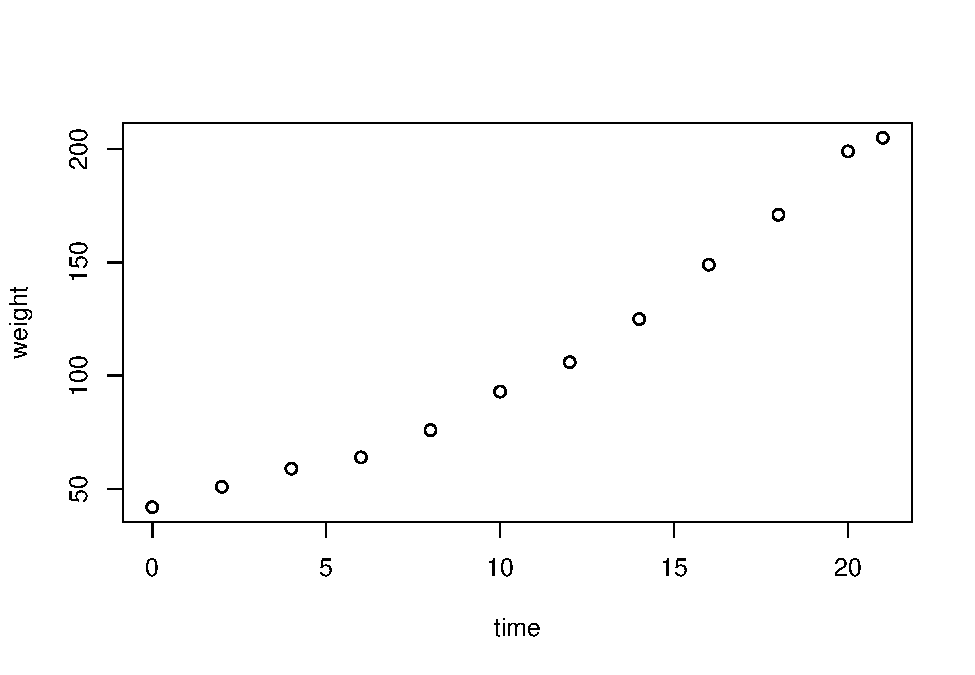
\includegraphics{01-intro_files/figure-latex/unnamed-chunk-2-1.pdf}
\item
  For a single variable a histogram summarizes the distribution of its observed values by counting the numer of observations in different intervals (buckets) of values. Keep in mind that histograms with different choices of buckets may look very different. Check out this histogram of ``Time 0'' weights of all 23 chicks.
  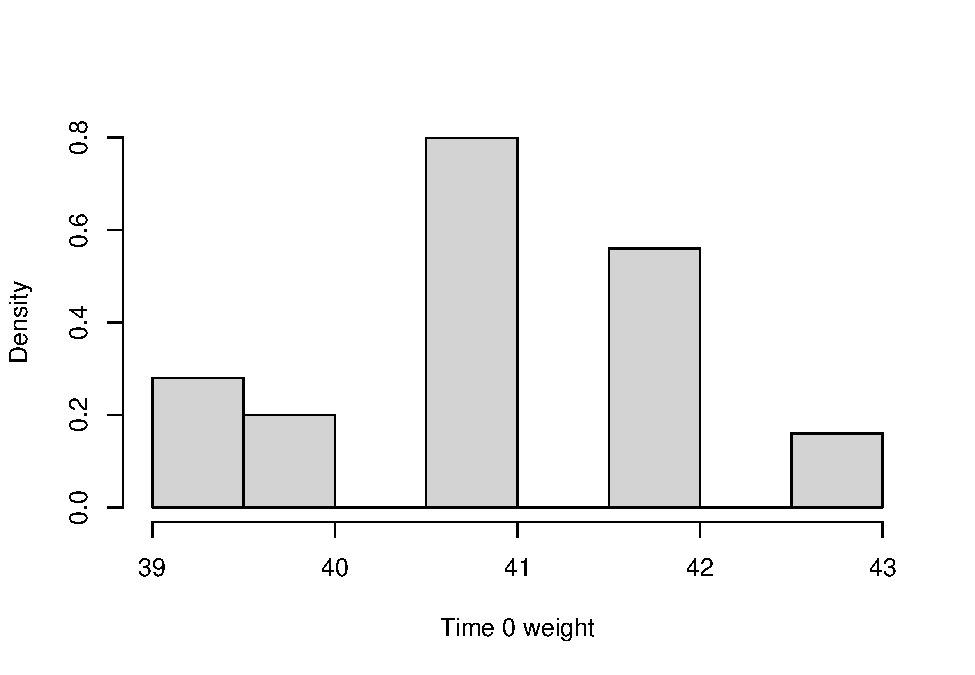
\includegraphics{01-intro_files/figure-latex/unnamed-chunk-3-1.pdf}
\item
  A qq-plot compares the shape of a distribution of observed values to another known distribution, often the standard normal distribution. For example, make the standardizing transformation \((x_i - \overline x) / \hat\sigma_x\) where \(x_i\) is the Time 0 weight of chick \(i\), \(\overline x\) is the observed mean and \(\hat\sigma_x\) is the observed standard deviation of those values. Compute the \(\alpha\) quantile of these values or several \(\alpha\) values in \((0,1)\) along with the corresponding standard normal quantiles (z-scores). Plot the pairs of \(\alpha\) quantiles in the xy-plane. If the standardized weights are approximately normal, then the points should lie approximately on the line \(y=x\). Note that extreme quantiles are always less reliably estimated, so it is typical for the ends of the ``line'' to fray up or down from the diagonal.
\end{itemize}

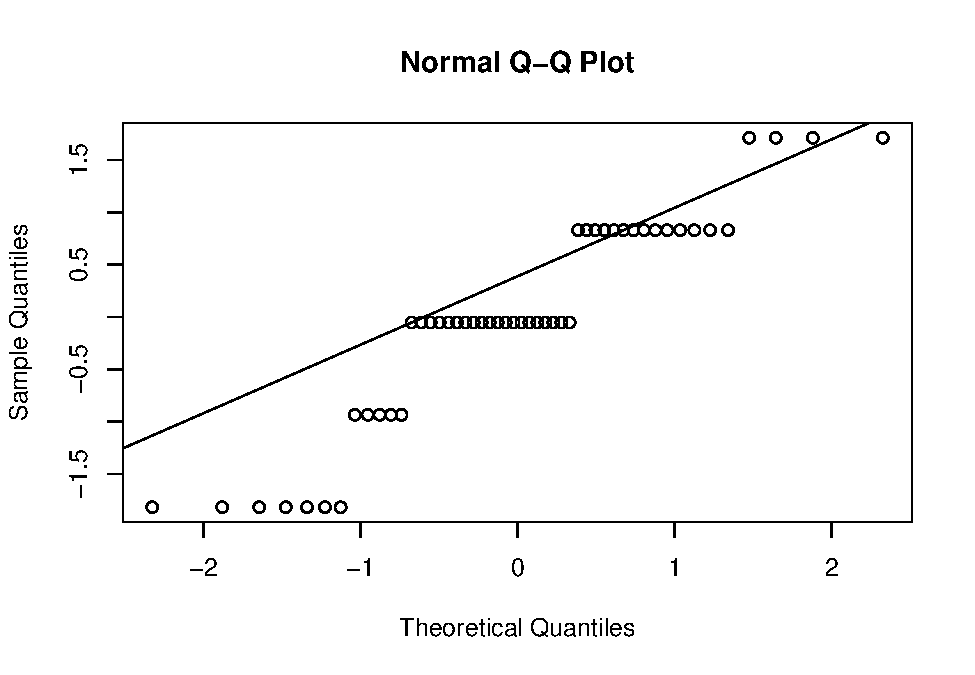
\includegraphics{01-intro_files/figure-latex/unnamed-chunk-4-1.pdf}

\hypertarget{statistical-inference}{%
\section{Statistical Inference}\label{statistical-inference}}

Summarizing data sets is important because no one can make sense of more than a few numbers at a time. But, data summaries cannot by themselves answer our research questions. That is because data summaries only say something about the particular data set we observe, while our research questions concern the whole population. Recall, a major aim of experimentation is generalizing from observations to population. When we make such generalizations we often refer to them as \emph{inferences}; and, statistical inferences are characterized by their careful treatment of statistical concepts, such as hypotheses, and Type 1 and 2 errors, which we discuss below.

A hypothesis is a claim or assertion about a population. These may be simple, i.e., ``the population mean is 5'', or more complex, like ``the population distribution of values is equivalent to a Normal probability distribution''. Notice that both of these statements are either true or false, yes or no. A hypothesis then may be called the ``null hypothesis'', and its complement (opposite) the alternative hypothesis. Which is which depends on the context. We make educated guesses about the truthfulness of a null hypothesis based on observations/data. Our educated guesses may be right or wrong, but we will never know because we will never ``see'' the whole population. If we reject the null hypothesis as false when it really is true, then we make a Type 1 error. The opposite, keeping the null hypothesis in favor over its alternative, when it is actually false, is a Type 2 error. Ideally, we would make no errors, but that's not possible. In fact, the two errors have an inverse relation. For example, if we adopt the rule that we always reject the null hypothesis, then we will necessarily maximize Type 1 errors but have no Type 2 errors. And, if we take the opposite approach, then we maximize Type 2 errors while making no Type 1 errors.

Much of this course will focus on constructing tests of relevant hypotheses with the property that we limit the chance of making a Type 1 error. By chance we refer to the probability distribution of the test outcome induced by random sampling of data from the population. A test that has chance no more than \(\alpha\) of making a Type 1 error is called a ``level \(\alpha\) test of \(H_0\)'', the null hypothesis.

\hypertarget{introduction-to-linear-models}{%
\chapter{Introduction to Linear Models}\label{introduction-to-linear-models}}

In this section we define linear models, provide simple examples, and analyze linear models for one- and two-sample problems.

\hypertarget{defining-the-linear-model}{%
\section{Defining the linear model}\label{defining-the-linear-model}}

Every linear model defines a linear relationship between an independent variable \(Y\) and a dependent variable \(X\), including a random term \(\epsilon\):
\begin{equation}
Y = X\beta + \epsilon
  \label{eq:linmod}
\end{equation}
Usually, \(X\) is a fixed or non-random variable, while \(\epsilon\) is a random variable representing variation due to a random sampling mechanism, so that \(Y\) is a random outcome. Further, in \eqref{eq:linmod} \(Y = (Y_1, \ldots, Y_n)^\top\) is an \(n\times 1\) vector of outcomes/responses, \(X\) is an \(n\times p\) matrix of fixed variables/covariates (\(p<n\)), \(\epsilon = (\epsilon_1, \ldots, \epsilon_n)^\top\) is an \(n\times 1\) vector of random variables, and \(\beta = (\beta_1, \ldots, \beta_p)^{\top}\) is a \(p\times 1\) coefficient vector of unknown parameters.

The \emph{least-squares model} or just called the \emph{linear model} is the above model with few or no additional assumptions although, to estimate the unknown parameter \(\beta\), which characterizes the relationship between \(X\) and \(Y\), assuming \(E(\epsilon_i) = 0\) is very helpful and usually reasonable.

The \emph{Gauss-Markov model}---which we will tacitly use throughout the course and examine in detail at the end of the semester---makes the assumptions \(E(\epsilon_i) = 0\), \(E(\epsilon_i^2) = \sigma^2\), which means the ``error'' term \(\epsilon\) has the same variance for each random sample (homogeneous or constant variance), and \(E(\epsilon_i\epsilon_j)=0\). Or, in other words, the last two assumptions may be written \(Cov(\epsilon) = \sigma^2 I_{n}\) where \(I_n\) is the \(n\times n\) identity matrix.

\hypertarget{gauss-markov-model-for-one-sample}{%
\section{Gauss-Markov model for one sample}\label{gauss-markov-model-for-one-sample}}

Let \(P\) be a normal population with mean \(\beta\) and variance \(\sigma^2\). Let \(Y_i\stackrel{iid}{\sim}P\). Then, we may write
\begin{equation}
\begin{aligned}
Y_i &= \beta x_i + \epsilon_i, \quad i = 1,\ldots, n, \,\,\text{or}\\
Y &= X\beta + \epsilon
\end{aligned}
\end{equation}
where \(x_i = 1\), so that \(X = (1, 1, ..., 1)^{\top}\) is an \(n\times 1\) vector of ones, and where \(\epsilon_i\stackrel{iid}{\sim}N(0,\sigma^2)\). This shows the Gauss-Markov model contains the one-sample normal population inference problem.

For inference on the population mean \(\beta\) we typically consider the point estimator \(\hat\beta = \overline Y\), the sample mean. And, we evaluate the usual one-sample Student's \(t\) test of \(H_0:\beta = \beta_0\) vs.~\(H_a:\beta\ne\beta_0\) by comparing the test statistic
\[T = \frac{\overline Y - \beta_0}{\sqrt{S^2/n}}\]
to quantiles of a Student's \(t\) distribution with \(n-1\) df, where \(S^2 = (n-1)^{-1}\sum_{i=1}^n(Y_i - \overline Y)^2\).

A common theme in the study and use of linear models is ``model-checking''. The idea is to us the data to interrogate the Gauss-Markov assumptions: linearity, normality, and constant variance (and sometimes independence). In the one-sample problem linearity is of no concern because \(x\) is constant, so there's no relationship between \(X\) and \(Y\) to check for linearity. Normality may be checked by constructing a qq-plot of the residuals \(\hat\epsilon_i = Y_i - \hat Y_i\) where \(\hat Y_i = \hat\beta x_i\); in this case, \(\hat\epsilon_i = Y_i - \overline Y\). Often times data exhibit non-homogeneous variance in the sense that the variance increases or decreases in \(X\). Again, this kind of non-homogeneity is not relevant in the one-sample problem. Finally, in data sets with time or space variation (like gasoline prices in Ames from 2021-2022), we may suspect non-independence of \(\epsilon_i\)'s. This kind of time-series dependence may be checked using a serial correlation plot; see below.

Example: A horticulturist plants 500 seeds of \emph{centaurea cyanus} in a 10 foot by 1 foot plot of clay-type soil in 1 foot by one foot squares. After 6 weeks she records the number of sprouted plants in each square, finding
\[37\,\,\, 24\,\,\, 31\,\,\, 21\,\,\,  9\,\,\, 21\,\,\, 15\,\,\, 37\,\,\, 31\,\,\, 26.\]
Assuming a normal population, she wants to infer the true average number of sprouted (germinated) seeds per one-foot by one-foot plot of fifty in clay-type soil.

In particular, she'd like to know if the true mean is at least 25. She will not make a wholesale purchase of this particular seed unless she is convinced the true mean is at least 25.

The horticulturist's Gauss-Markov model has \(Y_i\) equal to the recorded number of sprouts for sub-plots \(i=1, \ldots, 10\), and where \(x_i = 1\) for each. The following t-test concludes (at level 0.05) that the true mean is quite plausibly less than 25.

\begin{Shaded}
\begin{Highlighting}[]
\NormalTok{y }\OtherTok{\textless{}{-}} \FunctionTok{c}\NormalTok{(}\DecValTok{37}\NormalTok{, }\DecValTok{24}\NormalTok{, }\DecValTok{31}\NormalTok{, }\DecValTok{21}\NormalTok{,  }\DecValTok{9}\NormalTok{, }\DecValTok{21}\NormalTok{, }\DecValTok{15}\NormalTok{, }\DecValTok{37}\NormalTok{, }\DecValTok{31}\NormalTok{, }\DecValTok{26}\NormalTok{)}
\NormalTok{ybar }\OtherTok{\textless{}{-}} \FunctionTok{mean}\NormalTok{(y)}
\NormalTok{ybar}
\end{Highlighting}
\end{Shaded}

\begin{verbatim}
## [1] 25.2
\end{verbatim}

\begin{Shaded}
\begin{Highlighting}[]
\NormalTok{s2 }\OtherTok{\textless{}{-}} \FunctionTok{var}\NormalTok{(y)}
\NormalTok{s2}
\end{Highlighting}
\end{Shaded}

\begin{verbatim}
## [1] 83.28889
\end{verbatim}

\begin{Shaded}
\begin{Highlighting}[]
\NormalTok{n }\OtherTok{\textless{}{-}} \FunctionTok{length}\NormalTok{(y)}
\NormalTok{T }\OtherTok{\textless{}{-}}\NormalTok{ (ybar }\SpecialCharTok{{-}} \DecValTok{25}\NormalTok{)}\SpecialCharTok{/}\FunctionTok{sqrt}\NormalTok{(s2}\SpecialCharTok{/}\NormalTok{n)}
\NormalTok{T}
\end{Highlighting}
\end{Shaded}

\begin{verbatim}
## [1] 0.06930051
\end{verbatim}

\begin{Shaded}
\begin{Highlighting}[]
\FunctionTok{qt}\NormalTok{(}\FloatTok{0.95}\NormalTok{,n}\DecValTok{{-}1}\NormalTok{)}
\end{Highlighting}
\end{Shaded}

\begin{verbatim}
## [1] 1.833113
\end{verbatim}

\begin{Shaded}
\begin{Highlighting}[]
\DecValTok{1}\SpecialCharTok{{-}}\FunctionTok{pt}\NormalTok{(T,n}\DecValTok{{-}1}\NormalTok{)}
\end{Highlighting}
\end{Shaded}

\begin{verbatim}
## [1] 0.4731329
\end{verbatim}

\begin{Shaded}
\begin{Highlighting}[]
\NormalTok{ybar}\SpecialCharTok{+}\FunctionTok{qt}\NormalTok{(}\FunctionTok{c}\NormalTok{(}\FloatTok{0.025}\NormalTok{,}\FloatTok{0.975}\NormalTok{),n}\DecValTok{{-}1}\NormalTok{)}\SpecialCharTok{*}\FunctionTok{sqrt}\NormalTok{(s2}\SpecialCharTok{/}\NormalTok{n)}
\end{Highlighting}
\end{Shaded}

\begin{verbatim}
## [1] 18.67146 31.72854
\end{verbatim}

Further, we can interrogate the normality (Gaussianity) assumption using a qq-plot. The plot reveals no concerns about the normality assumption.

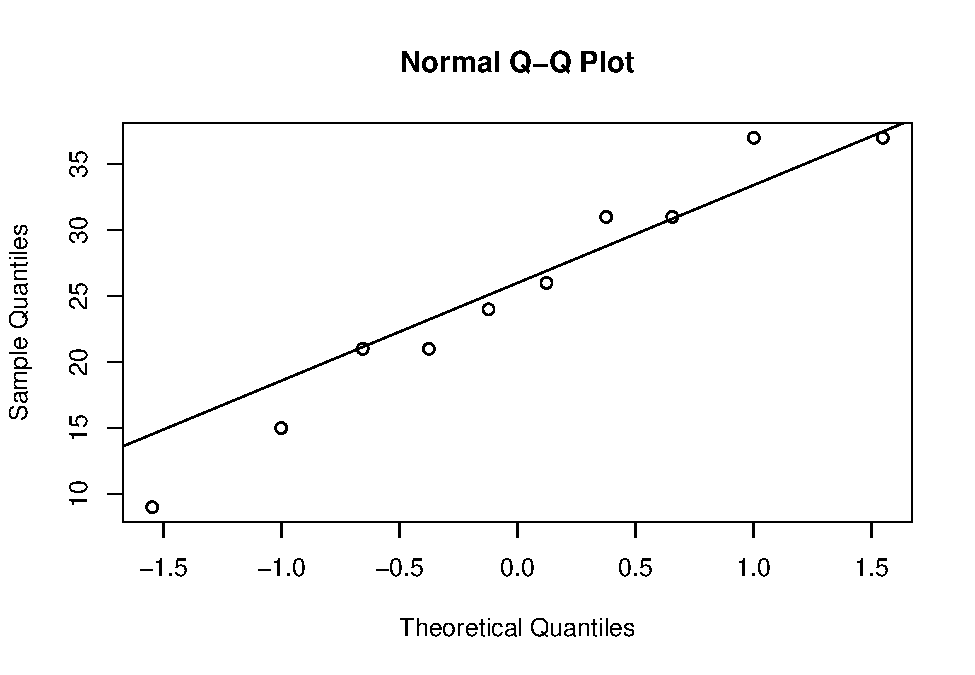
\includegraphics{02-Intro-to-Linear-Models_files/figure-latex/unnamed-chunk-2-1.pdf}

In this particular example, we may be concerned that sub-plots next to each other may have (spatially) correlated responses. One way to evaluate this is to compute the correlation between adjacent pairs. The observed (sample) correlation is only about \(12\%\), not high enough to suspect spatial non-independence.

\begin{Shaded}
\begin{Highlighting}[]
\NormalTok{y }\OtherTok{\textless{}{-}} \FunctionTok{c}\NormalTok{(}\DecValTok{37}\NormalTok{, }\DecValTok{24}\NormalTok{, }\DecValTok{31}\NormalTok{, }\DecValTok{21}\NormalTok{,  }\DecValTok{9}\NormalTok{, }\DecValTok{21}\NormalTok{, }\DecValTok{15}\NormalTok{, }\DecValTok{37}\NormalTok{, }\DecValTok{31}\NormalTok{, }\DecValTok{26}\NormalTok{)}
\NormalTok{n }\OtherTok{\textless{}{-}} \FunctionTok{length}\NormalTok{(y)}
\NormalTok{y\_adj }\OtherTok{\textless{}{-}} \FunctionTok{c}\NormalTok{(}\DecValTok{24}\NormalTok{, }\DecValTok{31}\NormalTok{, }\DecValTok{21}\NormalTok{,  }\DecValTok{9}\NormalTok{, }\DecValTok{21}\NormalTok{, }\DecValTok{15}\NormalTok{, }\DecValTok{37}\NormalTok{, }\DecValTok{31}\NormalTok{, }\DecValTok{26}\NormalTok{)}
\FunctionTok{cor}\NormalTok{(y[}\DecValTok{1}\SpecialCharTok{:}\NormalTok{(n}\DecValTok{{-}1}\NormalTok{)], y\_adj)}
\end{Highlighting}
\end{Shaded}

\begin{verbatim}
## [1] 0.1275145
\end{verbatim}

\hypertarget{gauss-markov-model-for-comparing-two-samples}{%
\section{Gauss-Markov model for comparing two samples}\label{gauss-markov-model-for-comparing-two-samples}}

Now suppose we have two normal populations, with the same variances, and we want to compare possibly different means. For some usual notation we might say \(X_{1,i}\stackrel{iid}{\sim}N(\mu_1, \sigma^2)\) for \(i=1, \ldots, n_1\) and \(X_{2,j}\stackrel{iid}{\sim}N(\mu_2, \sigma^2)\) for \(j=1, \ldots, n_2\). There are (at least) two ways to represent this data in linear model format. Either way, we let \(Y = (X_{1,1}, \ldots, X_{1,n_1}, X_{2,1}, \ldots, X_{2,n_2})^\top\) be the vector of \(n = n_1+n_2\) responses. The \emph{means model} uses design matrix \(X = (X_1, X_2)\) where \(X_1\) and \(X_2\) are \(n\times 1\) column vectors with \(X_1 = (1_{n_1}^\top, 0_{n_2}^\top)^{\top}\) and \(X_2 = (0_{n_1}^\top, 1_{n_2}^\top)^{\top}\). Suppose \(n_1 = n_2 = 10\); then, \(X\) looks like the following:

\begin{Shaded}
\begin{Highlighting}[]
\NormalTok{X }\OtherTok{=} \FunctionTok{cbind}\NormalTok{(}\FunctionTok{c}\NormalTok{(}\FunctionTok{rep}\NormalTok{(}\DecValTok{1}\NormalTok{,}\DecValTok{10}\NormalTok{),}\FunctionTok{rep}\NormalTok{(}\DecValTok{0}\NormalTok{,}\DecValTok{10}\NormalTok{)), }\FunctionTok{c}\NormalTok{(}\FunctionTok{rep}\NormalTok{(}\DecValTok{0}\NormalTok{,}\DecValTok{10}\NormalTok{),}\FunctionTok{rep}\NormalTok{(}\DecValTok{1}\NormalTok{,}\DecValTok{10}\NormalTok{)))}
\NormalTok{X}
\end{Highlighting}
\end{Shaded}

\begin{verbatim}
##       [,1] [,2]
##  [1,]    1    0
##  [2,]    1    0
##  [3,]    1    0
##  [4,]    1    0
##  [5,]    1    0
##  [6,]    1    0
##  [7,]    1    0
##  [8,]    1    0
##  [9,]    1    0
## [10,]    1    0
## [11,]    0    1
## [12,]    0    1
## [13,]    0    1
## [14,]    0    1
## [15,]    0    1
## [16,]    0    1
## [17,]    0    1
## [18,]    0    1
## [19,]    0    1
## [20,]    0    1
\end{verbatim}

The product \(X\beta\) is the vector \((\beta_1 1_{n_1}^\top, \beta_2 1_{n_2}^\top)^\top\). Taking the expectation of \(X\beta + \epsilon\) we get \(E(Y) = (\beta_1 1_{n_1}^\top, \beta_2 1_{n_2}^\top)^\top\). Therefore, \((\beta_1, \beta_2) = (\mu_1, \mu_2)\). In other words, the linear model coefficient vector is identical to the group means.

The second way to formulate the linear model is to encode the design matrix using the \emph{effects model}. Let \(X = (1_n^\top, (1_{n_1}^\top, 0_{n_2}^\top))^\top\), or, in other words:

\begin{Shaded}
\begin{Highlighting}[]
\NormalTok{X }\OtherTok{=} \FunctionTok{cbind}\NormalTok{(}\FunctionTok{rep}\NormalTok{(}\DecValTok{1}\NormalTok{,}\DecValTok{20}\NormalTok{), }\FunctionTok{c}\NormalTok{(}\FunctionTok{rep}\NormalTok{(}\DecValTok{1}\NormalTok{,}\DecValTok{10}\NormalTok{),}\FunctionTok{rep}\NormalTok{(}\DecValTok{0}\NormalTok{,}\DecValTok{10}\NormalTok{)))}
\NormalTok{X}
\end{Highlighting}
\end{Shaded}

\begin{verbatim}
##       [,1] [,2]
##  [1,]    1    1
##  [2,]    1    1
##  [3,]    1    1
##  [4,]    1    1
##  [5,]    1    1
##  [6,]    1    1
##  [7,]    1    1
##  [8,]    1    1
##  [9,]    1    1
## [10,]    1    1
## [11,]    1    0
## [12,]    1    0
## [13,]    1    0
## [14,]    1    0
## [15,]    1    0
## [16,]    1    0
## [17,]    1    0
## [18,]    1    0
## [19,]    1    0
## [20,]    1    0
\end{verbatim}

In that case, \(E(Y) = E(X\beta+\epsilon) = ((\beta_1 + \beta_2)1_{n_1}^\top, \beta_1 1_{n_2}^\top)^\top\). That means \(\beta_1 + \beta_2 = \mu_1\) and \(\beta_1 = \mu_2\). Or, equivalently, \(\beta_1 = \mu_2\) and \(\beta_2 = \mu_1 - \mu_2\). For this design, testing \(\beta_2=0\) is equivalent to testing for no difference in population means.

Example: The following is an analysis of carbon dioxide uptake rates of Echinochloa crus-galli grown in Quebec and Mississippi.

\begin{Shaded}
\begin{Highlighting}[]
\FunctionTok{boxplot}\NormalTok{(uptake}\SpecialCharTok{\textasciitilde{}}\NormalTok{Type, }\AttributeTok{data =}\NormalTok{ CO2)}
\end{Highlighting}
\end{Shaded}

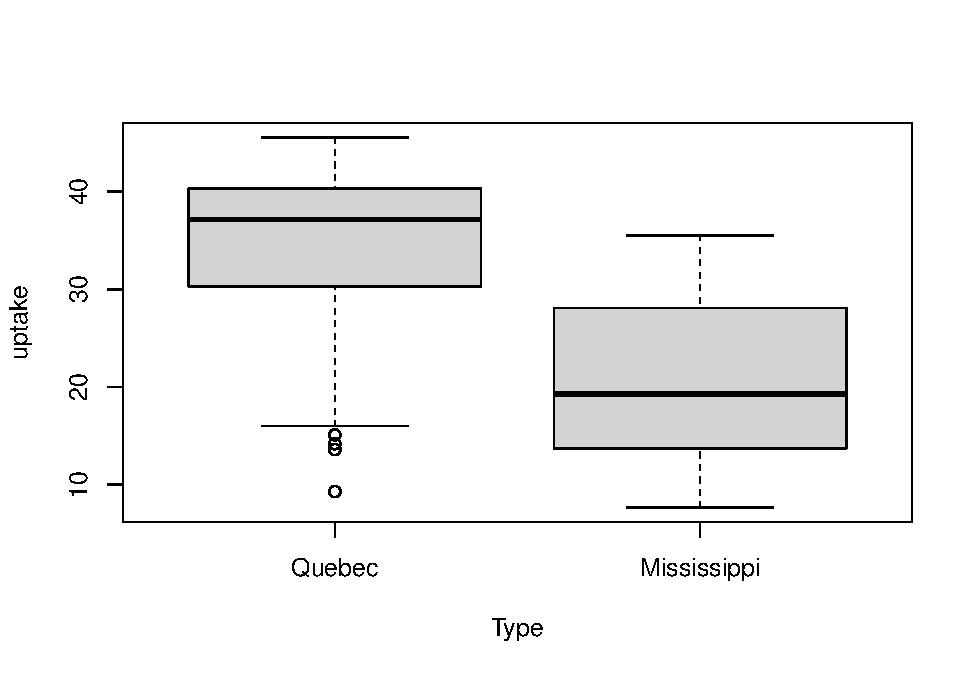
\includegraphics{02-Intro-to-Linear-Models_files/figure-latex/unnamed-chunk-6-1.pdf}

\begin{Shaded}
\begin{Highlighting}[]
\CommentTok{\# means model}
\NormalTok{hat.beta1 }\OtherTok{\textless{}{-}} \FunctionTok{mean}\NormalTok{(CO2}\SpecialCharTok{$}\NormalTok{uptake[CO2}\SpecialCharTok{$}\NormalTok{Type }\SpecialCharTok{==} \StringTok{\textquotesingle{}Quebec\textquotesingle{}}\NormalTok{])}
\NormalTok{hat.beta1}
\end{Highlighting}
\end{Shaded}

\begin{verbatim}
## [1] 33.54286
\end{verbatim}

\begin{Shaded}
\begin{Highlighting}[]
\NormalTok{hat.beta2 }\OtherTok{\textless{}{-}} \FunctionTok{mean}\NormalTok{(CO2}\SpecialCharTok{$}\NormalTok{uptake[CO2}\SpecialCharTok{$}\NormalTok{Type }\SpecialCharTok{==} \StringTok{\textquotesingle{}Mississippi\textquotesingle{}}\NormalTok{])}
\NormalTok{hat.beta2}
\end{Highlighting}
\end{Shaded}

\begin{verbatim}
## [1] 20.88333
\end{verbatim}

\begin{Shaded}
\begin{Highlighting}[]
\NormalTok{S2 }\OtherTok{\textless{}{-}}\NormalTok{ (}\FunctionTok{var}\NormalTok{(CO2}\SpecialCharTok{$}\NormalTok{uptake[CO2}\SpecialCharTok{$}\NormalTok{Type }\SpecialCharTok{==} \StringTok{\textquotesingle{}Quebec\textquotesingle{}}\NormalTok{]) }\SpecialCharTok{+} \FunctionTok{var}\NormalTok{(CO2}\SpecialCharTok{$}\NormalTok{uptake[CO2}\SpecialCharTok{$}\NormalTok{Type }\SpecialCharTok{==} \StringTok{\textquotesingle{}Mississippi\textquotesingle{}}\NormalTok{])) }\SpecialCharTok{/} \DecValTok{2}
\NormalTok{S2}
\end{Highlighting}
\end{Shaded}

\begin{verbatim}
## [1] 77.33465
\end{verbatim}

\begin{Shaded}
\begin{Highlighting}[]
\NormalTok{n }\OtherTok{\textless{}{-}} \FunctionTok{length}\NormalTok{(CO2}\SpecialCharTok{$}\NormalTok{uptake)}
\NormalTok{t }\OtherTok{=}\NormalTok{ (hat.beta1 }\SpecialCharTok{{-}}\NormalTok{ hat.beta2)}\SpecialCharTok{/}\FunctionTok{sqrt}\NormalTok{(S2}\SpecialCharTok{*}\NormalTok{(}\DecValTok{1}\SpecialCharTok{/}\NormalTok{(n}\SpecialCharTok{/}\DecValTok{2}\NormalTok{) }\SpecialCharTok{+} \DecValTok{1}\SpecialCharTok{/}\NormalTok{(n}\SpecialCharTok{/}\DecValTok{2}\NormalTok{)))}
\NormalTok{t}
\end{Highlighting}
\end{Shaded}

\begin{verbatim}
## [1] 6.596901
\end{verbatim}

\begin{Shaded}
\begin{Highlighting}[]
\DecValTok{1}\SpecialCharTok{{-}}\FunctionTok{pt}\NormalTok{(t, n}\DecValTok{{-}2}\NormalTok{)}
\end{Highlighting}
\end{Shaded}

\begin{verbatim}
## [1] 1.917343e-09
\end{verbatim}

\begin{Shaded}
\begin{Highlighting}[]
\FunctionTok{qt}\NormalTok{(}\FunctionTok{c}\NormalTok{(}\FloatTok{0.025}\NormalTok{,}\FloatTok{0.975}\NormalTok{),n}\DecValTok{{-}2}\NormalTok{)}
\end{Highlighting}
\end{Shaded}

\begin{verbatim}
## [1] -1.989319  1.989319
\end{verbatim}

\begin{Shaded}
\begin{Highlighting}[]
\NormalTok{residuals }\OtherTok{\textless{}{-}} \FunctionTok{c}\NormalTok{((CO2}\SpecialCharTok{$}\NormalTok{uptake[CO2}\SpecialCharTok{$}\NormalTok{Type }\SpecialCharTok{==} \StringTok{\textquotesingle{}Quebec\textquotesingle{}}\NormalTok{] }\SpecialCharTok{{-}}\NormalTok{ hat.beta1), CO2}\SpecialCharTok{$}\NormalTok{uptake[CO2}\SpecialCharTok{$}\NormalTok{Type }\SpecialCharTok{==} \StringTok{\textquotesingle{}Mississippi\textquotesingle{}}\NormalTok{] }\SpecialCharTok{{-}}\NormalTok{ hat.beta2)}
\NormalTok{studentized.residuals }\OtherTok{\textless{}{-}}\NormalTok{ residuals }\SpecialCharTok{/} \FunctionTok{sqrt}\NormalTok{(S2)}
\FunctionTok{qqplot}\NormalTok{(}\AttributeTok{x =} \FunctionTok{qt}\NormalTok{(}\FunctionTok{ppoints}\NormalTok{(}\DecValTok{500}\NormalTok{), }\AttributeTok{df =}\NormalTok{ n}\DecValTok{{-}2}\NormalTok{), studentized.residuals)}
\FunctionTok{qqline}\NormalTok{(studentized.residuals, }\AttributeTok{distribution =} \ControlFlowTok{function}\NormalTok{(p) }\FunctionTok{qt}\NormalTok{(p, }\AttributeTok{df =}\NormalTok{ n}\DecValTok{{-}2}\NormalTok{), }\AttributeTok{probs =} \FunctionTok{c}\NormalTok{(}\FloatTok{0.2}\NormalTok{, }\FloatTok{0.8}\NormalTok{), }\AttributeTok{col =} \DecValTok{2}\NormalTok{)}
\end{Highlighting}
\end{Shaded}

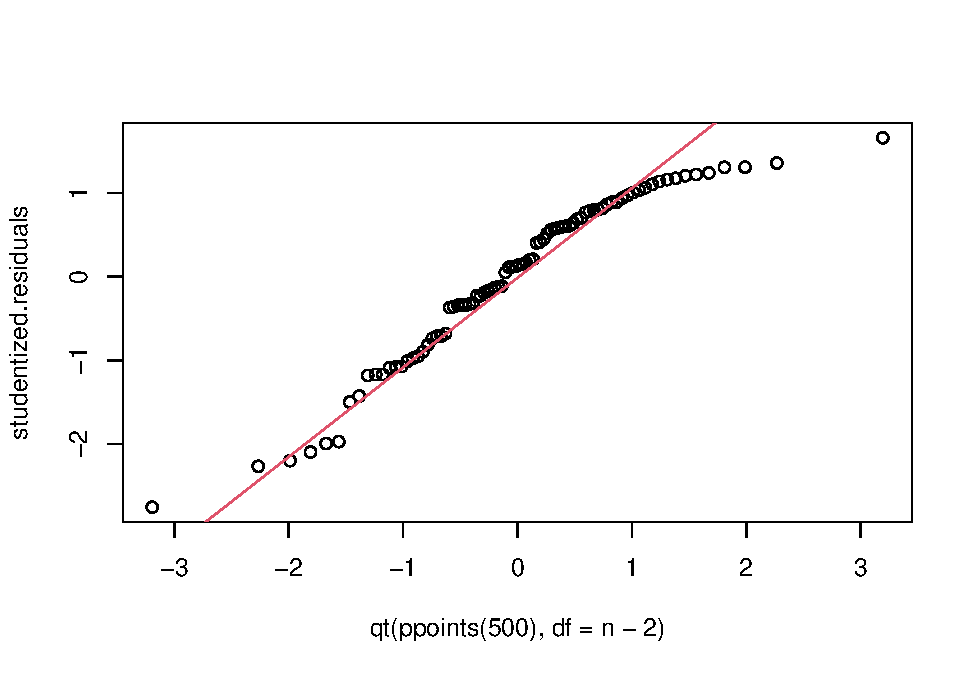
\includegraphics{02-Intro-to-Linear-Models_files/figure-latex/unnamed-chunk-6-2.pdf}

We conduct a two-sample t-test (assuming equal variances) and conclude there is a substantial difference in CO2 uptake of this grass species between the two locations. Inspection of the qq-plot reveals no concerns about normality.

\begin{Shaded}
\begin{Highlighting}[]
\CommentTok{\# Effects Model}
\FunctionTok{summary}\NormalTok{(}\FunctionTok{lm}\NormalTok{(uptake}\SpecialCharTok{\textasciitilde{}}\NormalTok{Type, }\AttributeTok{data =}\NormalTok{ CO2))}
\end{Highlighting}
\end{Shaded}

\begin{verbatim}
## 
## Call:
## lm(formula = uptake ~ Type, data = CO2)
## 
## Residuals:
##     Min      1Q  Median      3Q     Max 
## -24.243  -6.243   1.187   7.027  14.617 
## 
## Coefficients:
##                 Estimate Std. Error t value Pr(>|t|)    
## (Intercept)       33.543      1.357  24.719  < 2e-16 ***
## TypeMississippi  -12.660      1.919  -6.597 3.83e-09 ***
## ---
## Signif. codes:  0 '***' 0.001 '**' 0.01 '*' 0.05 '.' 0.1 ' ' 1
## 
## Residual standard error: 8.794 on 82 degrees of freedom
## Multiple R-squared:  0.3467, Adjusted R-squared:  0.3387 
## F-statistic: 43.52 on 1 and 82 DF,  p-value: 3.835e-09
\end{verbatim}

\begin{Shaded}
\begin{Highlighting}[]
\NormalTok{M }\OtherTok{\textless{}{-}} \FunctionTok{lm}\NormalTok{(uptake}\SpecialCharTok{\textasciitilde{}}\NormalTok{Type, }\AttributeTok{data =}\NormalTok{ CO2)}
\FunctionTok{model.matrix}\NormalTok{(M)}
\end{Highlighting}
\end{Shaded}

\begin{verbatim}
##    (Intercept) TypeMississippi
## 1            1               0
## 2            1               0
## 3            1               0
## 4            1               0
## 5            1               0
## 6            1               0
## 7            1               0
## 8            1               0
## 9            1               0
## 10           1               0
## 11           1               0
## 12           1               0
## 13           1               0
## 14           1               0
## 15           1               0
## 16           1               0
## 17           1               0
## 18           1               0
## 19           1               0
## 20           1               0
## 21           1               0
## 22           1               0
## 23           1               0
## 24           1               0
## 25           1               0
## 26           1               0
## 27           1               0
## 28           1               0
## 29           1               0
## 30           1               0
## 31           1               0
## 32           1               0
## 33           1               0
## 34           1               0
## 35           1               0
## 36           1               0
## 37           1               0
## 38           1               0
## 39           1               0
## 40           1               0
## 41           1               0
## 42           1               0
## 43           1               1
## 44           1               1
## 45           1               1
## 46           1               1
## 47           1               1
## 48           1               1
## 49           1               1
## 50           1               1
## 51           1               1
## 52           1               1
## 53           1               1
## 54           1               1
## 55           1               1
## 56           1               1
## 57           1               1
## 58           1               1
## 59           1               1
## 60           1               1
## 61           1               1
## 62           1               1
## 63           1               1
## 64           1               1
## 65           1               1
## 66           1               1
## 67           1               1
## 68           1               1
## 69           1               1
## 70           1               1
## 71           1               1
## 72           1               1
## 73           1               1
## 74           1               1
## 75           1               1
## 76           1               1
## 77           1               1
## 78           1               1
## 79           1               1
## 80           1               1
## 81           1               1
## 82           1               1
## 83           1               1
## 84           1               1
## attr(,"assign")
## [1] 0 1
## attr(,"contrasts")
## attr(,"contrasts")$Type
## [1] "contr.treatment"
\end{verbatim}

The \textbf{lm} function in R fits linear models and tests \(\beta_j = 0\) for each \(j=1, \ldots, p\). Note that the default design is a form of effects model, where the first level of the categorical variable is the baseline or reference level, so that the intercept term \(\beta_1\) is identified with its mean, while the other \(\beta\)'s become \emph{effects}, the differences \(\mu_2 - \mu_1\) and so on\ldots{}

\hypertarget{pairwise-testing-and-bonferroni-correction}{%
\section{Pairwise testing and Bonferroni correction}\label{pairwise-testing-and-bonferroni-correction}}

The two-sample t-test is appropriate for comparing two populations; for example, when experimenters compare two interventions/treatments in terms of mean effects. But, the two-sample t-test procedure does not generalize well to comparing 3 or more populations, i.e., more interventions. Let's see why not, and then consider what we could do instead.

Consider \(k\) treatments corresponding to \(k\) populations. Two sample t-tests may be used with the null hypothesis \(H_0:\mu_i = \mu_j\), \(i,j = 1, \ldots, k\), \(i\ne j\). There are \({k \choose 2}\) pairs of treatments, so there are the same number of tests to conduct. Now, suppose all the means are equal, i.e.~the treatments are indistinguishiable on the basis of mean. If each test is conducted at level \(\alpha\) then the chance of at least 1 type 1 error occurring is approximately \(1-(1-\alpha)^{{k \choose 2}}\), that is, if all tests are independent. For large \(k\), this \emph{familywise} type 1 error (type 1 error for all the tests) gets close to 1! In other words, the strategy of evaluating the hypothesis \(H_0:\text{all }\mu_i\text{'s are equal}\) by pairwise testing is not effective.

Several modifications are available to deal with this \emph{multiple testing problem}. We'll discuss two: Bonferroni and Benjamini-Hochberg adjustments. The Bonferroni adjustment requires the Type-1 error level \(\alpha\) of each test be changed to \(\alpha^\star = \alpha/k\) where \(k\) is the total number of tests. By the same probability calculation (assuming independence of tests) it follows that the family-wise type 1 error probability using the Bonferroni procedure is about \(\alpha\):
\begin{align*}
P(\text{at least one rejection given }H_0\text{ true}) &= 1-P(\text{no rejections given }H_0\text{ true})\\
& \stackrel{ind.}{=} 1-(1-\frac{\alpha}{k})^k\\
& \approx 1 - e^{-\alpha}\quad \text{for large k}\\
& \approx 1 - (1-\alpha) = \alpha \quad \text{for small }\alpha.
\end{align*}

The downside to Bonferroni is that when \(k\) is large each test has a very, very small chance of rejecting the null. In other words, each test has very low power. This inspired other procedures, like Benjamini-Hochberg (BH). Rather than controlling the family-wise type 1 error rate the BH procedure makes a compromise, and seeks to limit something called the false-discovery rate (FDR). Let \(V\) be the number of tests out of \(k\) that reject the null incorrectly, and let \(R\) be the number of tests out of \(k\) that reject the null. Then, FDR is defined as \(E(\frac{V}{R}|R>0)P(R>0)\). In words, the FDR is controlling the proportion of rejections that are incorrect out of all rejections, rather than out of all tests (like FWER does). If we did 1000 tests and rejected 40 nulls and controlled FDR at \(5\%\) we would expect 2 of the 40 rejections to be false rejections. To control FDR, the BH procedure instructs us to:
1. Sort the realized p-values from least to greatest \(p_{(1)}, p_{(2)}, ..., p_{(k)}\)
2. Find the largest \(\ell\) such that \(p_{(\ell)}\leq \frac{\ell}{k}\alpha\).
3. Reject all nulls corresponding to p-values \(p_{(1)}\) to \(p_{(\ell)}\).

\hypertarget{example-co2-uptake-in-echinochloa-crus-galli}{%
\subsection{Example: Co2 uptake in Echinochloa crus-galli}\label{example-co2-uptake-in-echinochloa-crus-galli}}

Consider the four interventions on the echinochloa grass formed by crossing the factors location and chilling with levels Mississippi/Quebec and chilled/non-chilled. We must make 6 pairwise comparisons, which we do below, using uncorrected, Bonferroni-corrected, and BH-corrected two-sample t-tests (assuming equal variances), and based on \(\alpha = 0.05\).

\begin{Shaded}
\begin{Highlighting}[]
\FunctionTok{library}\NormalTok{(datasets)}
\NormalTok{xbar1 }\OtherTok{\textless{}{-}} \FunctionTok{mean}\NormalTok{(CO2}\SpecialCharTok{$}\NormalTok{uptake[CO2}\SpecialCharTok{$}\NormalTok{Type}\SpecialCharTok{==}\StringTok{\textquotesingle{}Quebec\textquotesingle{}} \SpecialCharTok{\&}\NormalTok{ CO2}\SpecialCharTok{$}\NormalTok{Treatment }\SpecialCharTok{==} \StringTok{"chilled"}\NormalTok{])}
\NormalTok{xbar2 }\OtherTok{\textless{}{-}} \FunctionTok{mean}\NormalTok{(CO2}\SpecialCharTok{$}\NormalTok{uptake[CO2}\SpecialCharTok{$}\NormalTok{Type}\SpecialCharTok{==}\StringTok{\textquotesingle{}Quebec\textquotesingle{}} \SpecialCharTok{\&}\NormalTok{ CO2}\SpecialCharTok{$}\NormalTok{Treatment }\SpecialCharTok{==} \StringTok{"nonchilled"}\NormalTok{])}
\NormalTok{xbar3 }\OtherTok{\textless{}{-}} \FunctionTok{mean}\NormalTok{(CO2}\SpecialCharTok{$}\NormalTok{uptake[CO2}\SpecialCharTok{$}\NormalTok{Type}\SpecialCharTok{==}\StringTok{\textquotesingle{}Mississippi\textquotesingle{}} \SpecialCharTok{\&}\NormalTok{ CO2}\SpecialCharTok{$}\NormalTok{Treatment }\SpecialCharTok{==} \StringTok{"chilled"}\NormalTok{])}
\NormalTok{xbar4 }\OtherTok{\textless{}{-}} \FunctionTok{mean}\NormalTok{(CO2}\SpecialCharTok{$}\NormalTok{uptake[CO2}\SpecialCharTok{$}\NormalTok{Type}\SpecialCharTok{==}\StringTok{\textquotesingle{}Mississippi\textquotesingle{}} \SpecialCharTok{\&}\NormalTok{ CO2}\SpecialCharTok{$}\NormalTok{Treatment }\SpecialCharTok{==} \StringTok{"nonchilled"}\NormalTok{])}
\NormalTok{t1 }\OtherTok{\textless{}{-}}\NormalTok{ (xbar1 }\SpecialCharTok{{-}}\NormalTok{ xbar2)}\SpecialCharTok{/}\FunctionTok{sqrt}\NormalTok{((}\FloatTok{0.5}\SpecialCharTok{*}\NormalTok{(}\FunctionTok{var}\NormalTok{(CO2}\SpecialCharTok{$}\NormalTok{uptake[CO2}\SpecialCharTok{$}\NormalTok{Type}\SpecialCharTok{==}\StringTok{\textquotesingle{}Quebec\textquotesingle{}} \SpecialCharTok{\&}\NormalTok{ CO2}\SpecialCharTok{$}\NormalTok{Treatment }\SpecialCharTok{==} \StringTok{"chilled"}\NormalTok{]) }\SpecialCharTok{+} \FunctionTok{var}\NormalTok{(CO2}\SpecialCharTok{$}\NormalTok{uptake[CO2}\SpecialCharTok{$}\NormalTok{Type}\SpecialCharTok{==}\StringTok{\textquotesingle{}Quebec\textquotesingle{}} \SpecialCharTok{\&}\NormalTok{ CO2}\SpecialCharTok{$}\NormalTok{Treatment }\SpecialCharTok{==} \StringTok{"nonchilled"}\NormalTok{])))}\SpecialCharTok{*}\NormalTok{(}\DecValTok{1}\SpecialCharTok{/}\DecValTok{21} \SpecialCharTok{+} \DecValTok{1}\SpecialCharTok{/}\DecValTok{21}\NormalTok{))}
\NormalTok{t2 }\OtherTok{\textless{}{-}}\NormalTok{ (xbar1 }\SpecialCharTok{{-}}\NormalTok{ xbar3)}\SpecialCharTok{/}\FunctionTok{sqrt}\NormalTok{((}\FloatTok{0.5}\SpecialCharTok{*}\NormalTok{(}\FunctionTok{var}\NormalTok{(CO2}\SpecialCharTok{$}\NormalTok{uptake[CO2}\SpecialCharTok{$}\NormalTok{Type}\SpecialCharTok{==}\StringTok{\textquotesingle{}Quebec\textquotesingle{}} \SpecialCharTok{\&}\NormalTok{ CO2}\SpecialCharTok{$}\NormalTok{Treatment }\SpecialCharTok{==} \StringTok{"chilled"}\NormalTok{]) }\SpecialCharTok{+} \FunctionTok{var}\NormalTok{(CO2}\SpecialCharTok{$}\NormalTok{uptake[CO2}\SpecialCharTok{$}\NormalTok{Type}\SpecialCharTok{==}\StringTok{\textquotesingle{}Mississippi\textquotesingle{}} \SpecialCharTok{\&}\NormalTok{ CO2}\SpecialCharTok{$}\NormalTok{Treatment }\SpecialCharTok{==} \StringTok{"chilled"}\NormalTok{])))}\SpecialCharTok{*}\NormalTok{(}\DecValTok{1}\SpecialCharTok{/}\DecValTok{21} \SpecialCharTok{+} \DecValTok{1}\SpecialCharTok{/}\DecValTok{21}\NormalTok{))}
\NormalTok{t3 }\OtherTok{\textless{}{-}}\NormalTok{ (xbar1 }\SpecialCharTok{{-}}\NormalTok{ xbar4)}\SpecialCharTok{/}\FunctionTok{sqrt}\NormalTok{((}\FloatTok{0.5}\SpecialCharTok{*}\NormalTok{(}\FunctionTok{var}\NormalTok{(CO2}\SpecialCharTok{$}\NormalTok{uptake[CO2}\SpecialCharTok{$}\NormalTok{Type}\SpecialCharTok{==}\StringTok{\textquotesingle{}Quebec\textquotesingle{}} \SpecialCharTok{\&}\NormalTok{ CO2}\SpecialCharTok{$}\NormalTok{Treatment }\SpecialCharTok{==} \StringTok{"chilled"}\NormalTok{]) }\SpecialCharTok{+} \FunctionTok{var}\NormalTok{(CO2}\SpecialCharTok{$}\NormalTok{uptake[CO2}\SpecialCharTok{$}\NormalTok{Type}\SpecialCharTok{==}\StringTok{\textquotesingle{}Mississippi\textquotesingle{}} \SpecialCharTok{\&}\NormalTok{ CO2}\SpecialCharTok{$}\NormalTok{Treatment }\SpecialCharTok{==} \StringTok{"nonchilled"}\NormalTok{])))}\SpecialCharTok{*}\NormalTok{(}\DecValTok{1}\SpecialCharTok{/}\DecValTok{21} \SpecialCharTok{+} \DecValTok{1}\SpecialCharTok{/}\DecValTok{21}\NormalTok{))}
\NormalTok{t4 }\OtherTok{\textless{}{-}}\NormalTok{ (xbar2 }\SpecialCharTok{{-}}\NormalTok{ xbar3)}\SpecialCharTok{/}\FunctionTok{sqrt}\NormalTok{((}\FloatTok{0.5}\SpecialCharTok{*}\NormalTok{(}\FunctionTok{var}\NormalTok{(CO2}\SpecialCharTok{$}\NormalTok{uptake[CO2}\SpecialCharTok{$}\NormalTok{Type}\SpecialCharTok{==}\StringTok{\textquotesingle{}Quebec\textquotesingle{}} \SpecialCharTok{\&}\NormalTok{ CO2}\SpecialCharTok{$}\NormalTok{Treatment }\SpecialCharTok{==} \StringTok{"nonchilled"}\NormalTok{]) }\SpecialCharTok{+} \FunctionTok{var}\NormalTok{(CO2}\SpecialCharTok{$}\NormalTok{uptake[CO2}\SpecialCharTok{$}\NormalTok{Type}\SpecialCharTok{==}\StringTok{\textquotesingle{}Mississippi\textquotesingle{}} \SpecialCharTok{\&}\NormalTok{ CO2}\SpecialCharTok{$}\NormalTok{Treatment }\SpecialCharTok{==} \StringTok{"chilled"}\NormalTok{])))}\SpecialCharTok{*}\NormalTok{(}\DecValTok{1}\SpecialCharTok{/}\DecValTok{21} \SpecialCharTok{+} \DecValTok{1}\SpecialCharTok{/}\DecValTok{21}\NormalTok{))}
\NormalTok{t5 }\OtherTok{\textless{}{-}}\NormalTok{ (xbar2 }\SpecialCharTok{{-}}\NormalTok{ xbar4)}\SpecialCharTok{/}\FunctionTok{sqrt}\NormalTok{((}\FloatTok{0.5}\SpecialCharTok{*}\NormalTok{(}\FunctionTok{var}\NormalTok{(CO2}\SpecialCharTok{$}\NormalTok{uptake[CO2}\SpecialCharTok{$}\NormalTok{Type}\SpecialCharTok{==}\StringTok{\textquotesingle{}Quebec\textquotesingle{}} \SpecialCharTok{\&}\NormalTok{ CO2}\SpecialCharTok{$}\NormalTok{Treatment }\SpecialCharTok{==} \StringTok{"nonchilled"}\NormalTok{]) }\SpecialCharTok{+} \FunctionTok{var}\NormalTok{(CO2}\SpecialCharTok{$}\NormalTok{uptake[CO2}\SpecialCharTok{$}\NormalTok{Type}\SpecialCharTok{==}\StringTok{\textquotesingle{}Mississippi\textquotesingle{}} \SpecialCharTok{\&}\NormalTok{ CO2}\SpecialCharTok{$}\NormalTok{Treatment }\SpecialCharTok{==} \StringTok{"nonchilled"}\NormalTok{])))}\SpecialCharTok{*}\NormalTok{(}\DecValTok{1}\SpecialCharTok{/}\DecValTok{21} \SpecialCharTok{+} \DecValTok{1}\SpecialCharTok{/}\DecValTok{21}\NormalTok{))}
\NormalTok{t6 }\OtherTok{\textless{}{-}}\NormalTok{ (xbar3 }\SpecialCharTok{{-}}\NormalTok{ xbar4)}\SpecialCharTok{/}\FunctionTok{sqrt}\NormalTok{((}\FloatTok{0.5}\SpecialCharTok{*}\NormalTok{(}\FunctionTok{var}\NormalTok{(CO2}\SpecialCharTok{$}\NormalTok{uptake[CO2}\SpecialCharTok{$}\NormalTok{Type}\SpecialCharTok{==}\StringTok{\textquotesingle{}Mississippi\textquotesingle{}} \SpecialCharTok{\&}\NormalTok{ CO2}\SpecialCharTok{$}\NormalTok{Treatment }\SpecialCharTok{==} \StringTok{"chilled"}\NormalTok{]) }\SpecialCharTok{+} \FunctionTok{var}\NormalTok{(CO2}\SpecialCharTok{$}\NormalTok{uptake[CO2}\SpecialCharTok{$}\NormalTok{Type}\SpecialCharTok{==}\StringTok{\textquotesingle{}Mississippi\textquotesingle{}} \SpecialCharTok{\&}\NormalTok{ CO2}\SpecialCharTok{$}\NormalTok{Treatment }\SpecialCharTok{==} \StringTok{"nonchilled"}\NormalTok{])))}\SpecialCharTok{*}\NormalTok{(}\DecValTok{1}\SpecialCharTok{/}\DecValTok{21} \SpecialCharTok{+} \DecValTok{1}\SpecialCharTok{/}\DecValTok{21}\NormalTok{))}
\NormalTok{p1 }\OtherTok{\textless{}{-}} \DecValTok{2}\SpecialCharTok{*}\NormalTok{(}\DecValTok{1}\SpecialCharTok{{-}}\FunctionTok{pt}\NormalTok{(}\FunctionTok{abs}\NormalTok{(t1),}\DecValTok{40}\NormalTok{))}
\NormalTok{p2 }\OtherTok{\textless{}{-}} \DecValTok{2}\SpecialCharTok{*}\NormalTok{(}\DecValTok{1}\SpecialCharTok{{-}}\FunctionTok{pt}\NormalTok{(}\FunctionTok{abs}\NormalTok{(t2),}\DecValTok{40}\NormalTok{))}
\NormalTok{p3 }\OtherTok{\textless{}{-}} \DecValTok{2}\SpecialCharTok{*}\NormalTok{(}\DecValTok{1}\SpecialCharTok{{-}}\FunctionTok{pt}\NormalTok{(}\FunctionTok{abs}\NormalTok{(t3),}\DecValTok{40}\NormalTok{))}
\NormalTok{p4 }\OtherTok{\textless{}{-}} \DecValTok{2}\SpecialCharTok{*}\NormalTok{(}\DecValTok{1}\SpecialCharTok{{-}}\FunctionTok{pt}\NormalTok{(}\FunctionTok{abs}\NormalTok{(t4),}\DecValTok{40}\NormalTok{))}
\NormalTok{p5 }\OtherTok{\textless{}{-}} \DecValTok{2}\SpecialCharTok{*}\NormalTok{(}\DecValTok{1}\SpecialCharTok{{-}}\FunctionTok{pt}\NormalTok{(}\FunctionTok{abs}\NormalTok{(t5),}\DecValTok{40}\NormalTok{))}
\NormalTok{p6 }\OtherTok{\textless{}{-}} \DecValTok{2}\SpecialCharTok{*}\NormalTok{(}\DecValTok{1}\SpecialCharTok{{-}}\FunctionTok{pt}\NormalTok{(}\FunctionTok{abs}\NormalTok{(t6),}\DecValTok{40}\NormalTok{))}
\NormalTok{p1}
\end{Highlighting}
\end{Shaded}

\begin{verbatim}
## [1] 0.2348577
\end{verbatim}

\begin{Shaded}
\begin{Highlighting}[]
\NormalTok{p2}
\end{Highlighting}
\end{Shaded}

\begin{verbatim}
## [1] 2.000916e-08
\end{verbatim}

\begin{Shaded}
\begin{Highlighting}[]
\NormalTok{p3}
\end{Highlighting}
\end{Shaded}

\begin{verbatim}
## [1] 0.03471652
\end{verbatim}

\begin{Shaded}
\begin{Highlighting}[]
\NormalTok{p4}
\end{Highlighting}
\end{Shaded}

\begin{verbatim}
## [1] 1.297742e-10
\end{verbatim}

\begin{Shaded}
\begin{Highlighting}[]
\NormalTok{p5}
\end{Highlighting}
\end{Shaded}

\begin{verbatim}
## [1] 0.001011226
\end{verbatim}

\begin{Shaded}
\begin{Highlighting}[]
\NormalTok{p6}
\end{Highlighting}
\end{Shaded}

\begin{verbatim}
## [1] 2.355328e-06
\end{verbatim}

\begin{Shaded}
\begin{Highlighting}[]
\NormalTok{sorted }\OtherTok{\textless{}{-}} \FunctionTok{cbind}\NormalTok{(}\DecValTok{1}\SpecialCharTok{:}\DecValTok{6}\NormalTok{, }\FunctionTok{round}\NormalTok{(}\FunctionTok{c}\NormalTok{(p1,p2,p3,p4,p5,p6), }\DecValTok{4}\NormalTok{))}
\NormalTok{sorted }\OtherTok{\textless{}{-}}\NormalTok{ sorted[}\FunctionTok{order}\NormalTok{(sorted[,}\DecValTok{2}\NormalTok{]),]}
\FunctionTok{cbind}\NormalTok{(sorted,}\FunctionTok{c}\NormalTok{(}\FloatTok{0.05}\SpecialCharTok{/}\DecValTok{6}\NormalTok{,}\FloatTok{0.05}\SpecialCharTok{*}\DecValTok{2}\SpecialCharTok{/}\DecValTok{6}\NormalTok{,}\FloatTok{0.05}\SpecialCharTok{*}\DecValTok{3}\SpecialCharTok{/}\DecValTok{6}\NormalTok{,}\FloatTok{0.05}\SpecialCharTok{*}\DecValTok{4}\SpecialCharTok{/}\DecValTok{6}\NormalTok{,}\FloatTok{0.05}\SpecialCharTok{*}\DecValTok{5}\SpecialCharTok{/}\DecValTok{6}\NormalTok{,}\FloatTok{0.05}\SpecialCharTok{*}\DecValTok{6}\SpecialCharTok{/}\DecValTok{6}\NormalTok{), }\FunctionTok{c}\NormalTok{(sorted[}\DecValTok{1}\NormalTok{,}\DecValTok{2}\NormalTok{] }\SpecialCharTok{\textless{}=} \FloatTok{0.05}\SpecialCharTok{*}\DecValTok{1}\SpecialCharTok{/}\DecValTok{6}\NormalTok{, sorted[}\DecValTok{2}\NormalTok{,}\DecValTok{2}\NormalTok{] }\SpecialCharTok{\textless{}=} \FloatTok{0.05}\SpecialCharTok{*}\DecValTok{2}\SpecialCharTok{/}\DecValTok{6}\NormalTok{, sorted[}\DecValTok{3}\NormalTok{,}\DecValTok{2}\NormalTok{] }\SpecialCharTok{\textless{}=} \FloatTok{0.05}\SpecialCharTok{*}\DecValTok{3}\SpecialCharTok{/}\DecValTok{6}\NormalTok{, sorted[}\DecValTok{4}\NormalTok{,}\DecValTok{2}\NormalTok{] }\SpecialCharTok{\textless{}=} \FloatTok{0.05}\SpecialCharTok{*}\DecValTok{4}\SpecialCharTok{/}\DecValTok{6}\NormalTok{, sorted[}\DecValTok{5}\NormalTok{,}\DecValTok{2}\NormalTok{] }\SpecialCharTok{\textless{}=} \FloatTok{0.05}\SpecialCharTok{*}\DecValTok{5}\SpecialCharTok{/}\DecValTok{6}\NormalTok{, sorted[}\DecValTok{6}\NormalTok{,}\DecValTok{2}\NormalTok{] }\SpecialCharTok{\textless{}=} \FloatTok{0.05}\SpecialCharTok{*}\DecValTok{6}\SpecialCharTok{/}\DecValTok{6}\NormalTok{), }\FunctionTok{rep}\NormalTok{(}\FloatTok{0.05}\SpecialCharTok{/}\DecValTok{6}\NormalTok{,}\DecValTok{6}\NormalTok{),}
      \FunctionTok{c}\NormalTok{(sorted[}\DecValTok{1}\NormalTok{,}\DecValTok{2}\NormalTok{] }\SpecialCharTok{\textless{}=} \FloatTok{0.05}\SpecialCharTok{/}\DecValTok{6}\NormalTok{, sorted[}\DecValTok{2}\NormalTok{,}\DecValTok{2}\NormalTok{] }\SpecialCharTok{\textless{}=} \FloatTok{0.05}\SpecialCharTok{/}\DecValTok{6}\NormalTok{, sorted[}\DecValTok{3}\NormalTok{,}\DecValTok{2}\NormalTok{] }\SpecialCharTok{\textless{}=} \FloatTok{0.05}\SpecialCharTok{/}\DecValTok{6}\NormalTok{, sorted[}\DecValTok{4}\NormalTok{,}\DecValTok{2}\NormalTok{] }\SpecialCharTok{\textless{}=} \FloatTok{0.05}\SpecialCharTok{/}\DecValTok{6}\NormalTok{, sorted[}\DecValTok{5}\NormalTok{,}\DecValTok{2}\NormalTok{] }\SpecialCharTok{\textless{}=} \FloatTok{0.05}\SpecialCharTok{/}\DecValTok{6}\NormalTok{, sorted[}\DecValTok{6}\NormalTok{,}\DecValTok{2}\NormalTok{] }\SpecialCharTok{\textless{}=} \FloatTok{0.05}\SpecialCharTok{/}\DecValTok{6}\NormalTok{))}
\end{Highlighting}
\end{Shaded}

\begin{verbatim}
##      [,1]   [,2]        [,3] [,4]        [,5] [,6]
## [1,]    2 0.0000 0.008333333    1 0.008333333    1
## [2,]    4 0.0000 0.016666667    1 0.008333333    1
## [3,]    6 0.0000 0.025000000    1 0.008333333    1
## [4,]    5 0.0010 0.033333333    1 0.008333333    1
## [5,]    3 0.0347 0.041666667    1 0.008333333    0
## [6,]    1 0.2349 0.050000000    0 0.008333333    0
\end{verbatim}

Using uncorrected tests we would reject the null hypothesis in all but the first test. We actually get the same result using the BH procedure. but, the Bonferroni procedure is more conservative and does not allow us to reject the null in the 1st or 3rd tests.

\hypertarget{linear-models-for-more-than-two-treatments-populations}{%
\section{Linear Models for more than two treatments (populations)}\label{linear-models-for-more-than-two-treatments-populations}}

We may generalize the ``means model'' and ``effects model'' constructions to apply the Gauss-Markov model to data sets with several treatments, as in the CO2 data set considered above. Recall that the CO2 data set has 84 observations, 21 in each of four groups: Quebec-chilled, Quebec-nonchilled, Mississippi-chilled, and Mississippi-nonchilled. If we sort the response vector to correspond to these categories, we can construct the design matrix as follows: \(X = (X_1, X_2, X_3, X_4)\) where \(X_1\) is the \(84\times 1\) column vector combined by stacking a \(21\times 1\) vector of 1's atop a \(63\times 1\) vector of 0's. The remaining columns of \(X\) are formed analogously, with the 21 1 values occupying the 22nd through 42nd spots, the 43rd through 63rd, and the 64th through 84th, respectively.

\begin{Shaded}
\begin{Highlighting}[]
\NormalTok{X }\OtherTok{\textless{}{-}} \FunctionTok{cbind}\NormalTok{(  }\FunctionTok{c}\NormalTok{(}\FunctionTok{rep}\NormalTok{(}\DecValTok{1}\NormalTok{,}\DecValTok{21}\NormalTok{),}\FunctionTok{rep}\NormalTok{(}\DecValTok{0}\NormalTok{,}\DecValTok{21}\NormalTok{),}\FunctionTok{rep}\NormalTok{(}\DecValTok{0}\NormalTok{,}\DecValTok{21}\NormalTok{),}\FunctionTok{rep}\NormalTok{(}\DecValTok{0}\NormalTok{,}\DecValTok{21}\NormalTok{)),}
             \FunctionTok{c}\NormalTok{(}\FunctionTok{rep}\NormalTok{(}\DecValTok{0}\NormalTok{,}\DecValTok{21}\NormalTok{),}\FunctionTok{rep}\NormalTok{(}\DecValTok{1}\NormalTok{,}\DecValTok{21}\NormalTok{),}\FunctionTok{rep}\NormalTok{(}\DecValTok{0}\NormalTok{,}\DecValTok{21}\NormalTok{),}\FunctionTok{rep}\NormalTok{(}\DecValTok{0}\NormalTok{,}\DecValTok{21}\NormalTok{)),}
             \FunctionTok{c}\NormalTok{(}\FunctionTok{rep}\NormalTok{(}\DecValTok{0}\NormalTok{,}\DecValTok{21}\NormalTok{),}\FunctionTok{rep}\NormalTok{(}\DecValTok{0}\NormalTok{,}\DecValTok{21}\NormalTok{),}\FunctionTok{rep}\NormalTok{(}\DecValTok{1}\NormalTok{,}\DecValTok{21}\NormalTok{),}\FunctionTok{rep}\NormalTok{(}\DecValTok{0}\NormalTok{,}\DecValTok{21}\NormalTok{)),}
             \FunctionTok{c}\NormalTok{(}\FunctionTok{rep}\NormalTok{(}\DecValTok{0}\NormalTok{,}\DecValTok{21}\NormalTok{),}\FunctionTok{rep}\NormalTok{(}\DecValTok{0}\NormalTok{,}\DecValTok{21}\NormalTok{),}\FunctionTok{rep}\NormalTok{(}\DecValTok{0}\NormalTok{,}\DecValTok{21}\NormalTok{),}\FunctionTok{rep}\NormalTok{(}\DecValTok{1}\NormalTok{,}\DecValTok{21}\NormalTok{)))}
\end{Highlighting}
\end{Shaded}

This construction is a ``means model'' matrix because the coefficient vector \(\beta\) is identified with the four group means. That is, \(X\beta = (\beta_1 1_{21\times1}^\top, \beta_2 1_{21\times1}^\top, \beta_3 1_{21\times1}^\top, \beta_4 1_{21\times1}^\top)^\top\). So, \(\beta_j = \mu_j\) for \(j=1,...,4\).

There are many ways to define an ``effects model'' for the CO2 dataset. Recall that R uses an effects model parametrization by default. Let's fit a linear model in R and see what model matrix R constructs.

\begin{Shaded}
\begin{Highlighting}[]
\FunctionTok{library}\NormalTok{(datasets)}
\NormalTok{CO2subset }\OtherTok{\textless{}{-}} \FunctionTok{data.frame}\NormalTok{(CO2}\SpecialCharTok{$}\NormalTok{Type, CO2}\SpecialCharTok{$}\NormalTok{Treatment,  CO2}\SpecialCharTok{$}\NormalTok{uptake)}
\NormalTok{my.lm }\OtherTok{\textless{}{-}} \FunctionTok{lm}\NormalTok{(CO2.uptake}\SpecialCharTok{\textasciitilde{}}\NormalTok{CO2.Type}\SpecialCharTok{+}\NormalTok{CO2.Treatment, }\AttributeTok{data =}\NormalTok{ CO2subset)}
\FunctionTok{model.matrix}\NormalTok{(my.lm)}
\end{Highlighting}
\end{Shaded}

\begin{verbatim}
##    (Intercept) CO2.TypeMississippi CO2.Treatmentchilled
## 1            1                   0                    0
## 2            1                   0                    0
## 3            1                   0                    0
## 4            1                   0                    0
## 5            1                   0                    0
## 6            1                   0                    0
## 7            1                   0                    0
## 8            1                   0                    0
## 9            1                   0                    0
## 10           1                   0                    0
## 11           1                   0                    0
## 12           1                   0                    0
## 13           1                   0                    0
## 14           1                   0                    0
## 15           1                   0                    0
## 16           1                   0                    0
## 17           1                   0                    0
## 18           1                   0                    0
## 19           1                   0                    0
## 20           1                   0                    0
## 21           1                   0                    0
## 22           1                   0                    1
## 23           1                   0                    1
## 24           1                   0                    1
## 25           1                   0                    1
## 26           1                   0                    1
## 27           1                   0                    1
## 28           1                   0                    1
## 29           1                   0                    1
## 30           1                   0                    1
## 31           1                   0                    1
## 32           1                   0                    1
## 33           1                   0                    1
## 34           1                   0                    1
## 35           1                   0                    1
## 36           1                   0                    1
## 37           1                   0                    1
## 38           1                   0                    1
## 39           1                   0                    1
## 40           1                   0                    1
## 41           1                   0                    1
## 42           1                   0                    1
## 43           1                   1                    0
## 44           1                   1                    0
## 45           1                   1                    0
## 46           1                   1                    0
## 47           1                   1                    0
## 48           1                   1                    0
## 49           1                   1                    0
## 50           1                   1                    0
## 51           1                   1                    0
## 52           1                   1                    0
## 53           1                   1                    0
## 54           1                   1                    0
## 55           1                   1                    0
## 56           1                   1                    0
## 57           1                   1                    0
## 58           1                   1                    0
## 59           1                   1                    0
## 60           1                   1                    0
## 61           1                   1                    0
## 62           1                   1                    0
## 63           1                   1                    0
## 64           1                   1                    1
## 65           1                   1                    1
## 66           1                   1                    1
## 67           1                   1                    1
## 68           1                   1                    1
## 69           1                   1                    1
## 70           1                   1                    1
## 71           1                   1                    1
## 72           1                   1                    1
## 73           1                   1                    1
## 74           1                   1                    1
## 75           1                   1                    1
## 76           1                   1                    1
## 77           1                   1                    1
## 78           1                   1                    1
## 79           1                   1                    1
## 80           1                   1                    1
## 81           1                   1                    1
## 82           1                   1                    1
## 83           1                   1                    1
## 84           1                   1                    1
## attr(,"assign")
## [1] 0 1 2
## attr(,"contrasts")
## attr(,"contrasts")$CO2.Type
## [1] "contr.treatment"
## 
## attr(,"contrasts")$CO2.Treatment
## [1] "contr.treatment"
\end{verbatim}

Based on the model matrix, we see that R defines three coefficients, \(\beta_1, \beta_2, \beta_3\).

\hypertarget{randomization-and-permutation-testing}{%
\chapter{Randomization and Permutation Testing}\label{randomization-and-permutation-testing}}

\hypertarget{setup}{%
\section{Setup}\label{setup}}

Randomization/permutation testing is performed in the context of randomized intervention experiments or observational studies to examine the differences in response between two groups. The setting is similar to the setting in which the two-sample t-test is often used, but there are few other similarities.\\
A general algorithm for a randomization test of two groups, labelled, say, 0 and 1, is as follows:
1. Choose some statistic, say \(T\), quantifying the response difference between the groups and compute this \(T = t_0\) for the observed data.
For m in 1:M repeat:
2. Permute the 0,1 labels of the responses. If the data comes from a randomized experiment this is like saying the randomization of subjects to treatments turned out differently, hence the name randomization test.
3. Compute the \(m^{th}\) statistic value \(t_m\) on the responses with permuted/re-randomized labels.

At the end of this algorithm we end up with the values \(t_1, \ldots, t_m\). What do we make of these? Here's the idea. For a concrete example, suppose \(T\) is the Student's \(t\) two-sample test statistic, i.e., \(T = \frac{\overline x_0 - \overline x_1}{\sqrt{S_0^2/n_0 + S_1^2/n_1}}\). Let \(x\) denote all the responses of both groups pooled together, i.e., \(x = (x_{0,1}, ..., x_{0,n_0}, x_{1,1}, ...,x_{1,n_1})\). \(x\) has some sample mean value; call it \(\overline x\). If we randomly label \(n_0\) of the x's 0 and the other \(n_1\) of them 1, we should expect the average value of \(\overline x_0 - \overline x_1\) to be about 0 when averaging over repeated re-labeling. That's because \(\overline x_0\) and \(\overline x_1\) are both approximately unbiased for \(\overline x\). So the distribution/histogram of the \(t_1, ..., t_m\) values will look roughly symmetric around zero. Then, we compare the observed value \(t_0\) to this distribution and observe whether \(t_0\) is a ``typical'' value or and ``extreme'' value compared to \(t_1, ..., t_m\); that is, we compare \(t_0\) the the quantiles of \(t_1, ..., t_m\). If \(t_0\) is extreme compared to these values, then either we observed such a value by a small chance or the labels really do have an effect on the responses which is reflected in the statistic \(T\).

This description should sound very similar to null hypothesis testing and rejection rules defined by comparing a test statistic to a null distribution. But,there are some differences. In this case, the ``population'' consists only of the observed values. And, the \emph{randomization distribution}---the histogram/quantiles of \(t_1, ..., t_m\)---is only related to the observed data, not any larger population. This means that the ``null hypothesis'' that a randomization test tests is related only to the observed data. I think of the null and alternative hypotheses as the following: \(H_0: \text{the observed value } t_0 \text{ is consistent with labels being randomly assigned to responses}\) versus \(H_a: \text{the observed value } t_0 \text{ is NOT consistent with labels being randomly assigned to responses}\). Because the test references no population, the conclusion is only pertinent to the sampled subjects. If the original labels were assigned by randomization (i.e., they represent an intervention) then the conclusion may claim causation.

\hypertarget{example-1-the-harris-bank-sex-pay-study}{%
\subsection{Example 1: The Harris Bank Sex Pay Study}\label{example-1-the-harris-bank-sex-pay-study}}

We have worked with this data before: there are 93 salaries of Harris Bank employees from 1969-1971. The workers are all entry-level clerical workers. We're interested in whether males and females are paid differently.

\begin{Shaded}
\begin{Highlighting}[]
\NormalTok{salaries.df }\OtherTok{\textless{}{-}} \FunctionTok{read.csv}\NormalTok{(}\StringTok{\textquotesingle{}salaries.csv\textquotesingle{}}\NormalTok{)}
\NormalTok{salaries.df}
\end{Highlighting}
\end{Shaded}

\begin{verbatim}
##    Salary Sex
## 1    4620   1
## 2    5040   1
## 3    5100   1
## 4    5100   1
## 5    5220   1
## 6    5400   1
## 7    5400   1
## 8    5400   1
## 9    5400   1
## 10   5400   1
## 11   5700   1
## 12   6000   1
## 13   6000   1
## 14   6000   1
## 15   6000   1
## 16   6000   1
## 17   6000   1
## 18   6000   1
## 19   6000   1
## 20   6000   1
## 21   6000   1
## 22   6000   1
## 23   6000   1
## 24   6000   1
## 25   6300   1
## 26   6600   1
## 27   6600   1
## 28   6600   1
## 29   6840   1
## 30   6900   1
## 31   6900   1
## 32   8100   1
## 33   3900   0
## 34   4020   0
## 35   4290   0
## 36   4380   0
## 37   4380   0
## 38   4380   0
## 39   4380   0
## 40   4380   0
## 41   4440   0
## 42   4500   0
## 43   4500   0
## 44   4620   0
## 45   4800   0
## 46   4800   0
## 47   4800   0
## 48   4800   0
## 49   4800   0
## 50   4800   0
## 51   4800   0
## 52   4800   0
## 53   4800   0
## 54   4800   0
## 55   4980   0
## 56   5100   0
## 57   5100   0
## 58   5100   0
## 59   5100   0
## 60   5100   0
## 61   5100   0
## 62   5160   0
## 63   5220   0
## 64   5220   0
## 65   5280   0
## 66   5280   0
## 67   5280   0
## 68   5400   0
## 69   5400   0
## 70   5400   0
## 71   5400   0
## 72   5400   0
## 73   5400   0
## 74   5400   0
## 75   5400   0
## 76   5400   0
## 77   5400   0
## 78   5400   0
## 79   5400   0
## 80   5520   0
## 81   5520   0
## 82   5580   0
## 83   5640   0
## 84   5700   0
## 85   5700   0
## 86   5700   0
## 87   5700   0
## 88   5700   0
## 89   6000   0
## 90   6000   0
## 91   6120   0
## 92   6300   0
## 93   6300   0
\end{verbatim}

\hypertarget{difference-in-mean-salaries-between-genders}{%
\subsection{Difference in mean salaries between genders}\label{difference-in-mean-salaries-between-genders}}

\begin{Shaded}
\begin{Highlighting}[]
\NormalTok{n0 }\OtherTok{\textless{}{-}} \FunctionTok{sum}\NormalTok{(salaries.df}\SpecialCharTok{$}\NormalTok{Sex}\SpecialCharTok{==}\DecValTok{0}\NormalTok{)}
\NormalTok{n1 }\OtherTok{\textless{}{-}} \FunctionTok{sum}\NormalTok{(salaries.df}\SpecialCharTok{$}\NormalTok{Sex}\SpecialCharTok{==}\DecValTok{1}\NormalTok{)}
\NormalTok{m0 }\OtherTok{\textless{}{-}} \FunctionTok{mean}\NormalTok{(salaries.df}\SpecialCharTok{$}\NormalTok{Salary[salaries.df}\SpecialCharTok{$}\NormalTok{Sex}\SpecialCharTok{==}\DecValTok{0}\NormalTok{])}
\NormalTok{m1 }\OtherTok{\textless{}{-}} \FunctionTok{mean}\NormalTok{(salaries.df}\SpecialCharTok{$}\NormalTok{Salary[salaries.df}\SpecialCharTok{$}\NormalTok{Sex}\SpecialCharTok{==}\DecValTok{1}\NormalTok{])}
\NormalTok{s0 }\OtherTok{\textless{}{-}} \FunctionTok{var}\NormalTok{(salaries.df}\SpecialCharTok{$}\NormalTok{Salary[salaries.df}\SpecialCharTok{$}\NormalTok{Sex}\SpecialCharTok{==}\DecValTok{0}\NormalTok{])}
\NormalTok{s1 }\OtherTok{\textless{}{-}} \FunctionTok{var}\NormalTok{(salaries.df}\SpecialCharTok{$}\NormalTok{Salary[salaries.df}\SpecialCharTok{$}\NormalTok{Sex}\SpecialCharTok{==}\DecValTok{1}\NormalTok{])}
\NormalTok{t0 }\OtherTok{\textless{}{-}}\NormalTok{ (m0 }\SpecialCharTok{{-}}\NormalTok{ m1)}\SpecialCharTok{/}\FunctionTok{sqrt}\NormalTok{(s0}\SpecialCharTok{/}\NormalTok{n0}\SpecialCharTok{+}\NormalTok{s1}\SpecialCharTok{/}\NormalTok{n1)}
\FunctionTok{c}\NormalTok{(t0,m0,m1,}\FunctionTok{sqrt}\NormalTok{(s0),}\FunctionTok{sqrt}\NormalTok{(s1))}
\end{Highlighting}
\end{Shaded}

\begin{verbatim}
## [1]   -5.829974 5138.852459 5956.875000  539.870658  690.733306
\end{verbatim}

\hypertarget{randomization-test-for-treatment-significance}{%
\subsection{Randomization test for treatment significance}\label{randomization-test-for-treatment-significance}}

Algorithm:
for 1000 loops do:
1. randomly shuffle the sex labels over salaries
2. compute the two-sample t-test stat for the reshuffled labels
return all 1000 differences

\begin{Shaded}
\begin{Highlighting}[]
\NormalTok{n0 }\OtherTok{\textless{}{-}} \FunctionTok{sum}\NormalTok{(salaries.df}\SpecialCharTok{$}\NormalTok{Sex}\SpecialCharTok{==}\DecValTok{0}\NormalTok{)}
\NormalTok{n1 }\OtherTok{\textless{}{-}} \FunctionTok{sum}\NormalTok{(salaries.df}\SpecialCharTok{$}\NormalTok{Sex}\SpecialCharTok{==}\DecValTok{1}\NormalTok{)}
\NormalTok{n }\OtherTok{\textless{}{-}}\NormalTok{ n0}\SpecialCharTok{+}\NormalTok{n1}
\NormalTok{randomization.test }\OtherTok{\textless{}{-}} \ControlFlowTok{function}\NormalTok{(M)\{}
\NormalTok{  ts }\OtherTok{\textless{}{-}} \FunctionTok{rep}\NormalTok{(}\ConstantTok{NA}\NormalTok{,M)}
  \ControlFlowTok{for}\NormalTok{(m }\ControlFlowTok{in} \DecValTok{1}\SpecialCharTok{:}\NormalTok{M)\{}
\NormalTok{    permute.n }\OtherTok{\textless{}{-}} \FunctionTok{sample.int}\NormalTok{(n,n,}\AttributeTok{replace =}\NormalTok{ F)}
\NormalTok{    re.randomized.group }\OtherTok{\textless{}{-}}\NormalTok{ salaries.df}\SpecialCharTok{$}\NormalTok{Sex[permute.n]}
\NormalTok{    m0 }\OtherTok{\textless{}{-}} \FunctionTok{mean}\NormalTok{(salaries.df}\SpecialCharTok{$}\NormalTok{Salary[re.randomized.group}\SpecialCharTok{==}\DecValTok{0}\NormalTok{])}
\NormalTok{    m1 }\OtherTok{\textless{}{-}} \FunctionTok{mean}\NormalTok{(salaries.df}\SpecialCharTok{$}\NormalTok{Salary[re.randomized.group}\SpecialCharTok{==}\DecValTok{1}\NormalTok{])}
\NormalTok{    s0 }\OtherTok{\textless{}{-}} \FunctionTok{var}\NormalTok{(salaries.df}\SpecialCharTok{$}\NormalTok{Salary[re.randomized.group}\SpecialCharTok{==}\DecValTok{0}\NormalTok{])}
\NormalTok{    s1 }\OtherTok{\textless{}{-}} \FunctionTok{var}\NormalTok{(salaries.df}\SpecialCharTok{$}\NormalTok{Salary[re.randomized.group}\SpecialCharTok{==}\DecValTok{1}\NormalTok{])}
\NormalTok{    ts[m] }\OtherTok{\textless{}{-}}\NormalTok{ (m0 }\SpecialCharTok{{-}}\NormalTok{ m1)}\SpecialCharTok{/}\FunctionTok{sqrt}\NormalTok{(s0}\SpecialCharTok{/}\NormalTok{n0}\SpecialCharTok{+}\NormalTok{s1}\SpecialCharTok{/}\NormalTok{n1)}
\NormalTok{    \}}
  \FunctionTok{return}\NormalTok{(ts)}
\NormalTok{\}}

\NormalTok{ts }\OtherTok{\textless{}{-}} \FunctionTok{randomization.test}\NormalTok{(}\DecValTok{1000}\NormalTok{)}
\FunctionTok{hist}\NormalTok{(ts)}
\FunctionTok{abline}\NormalTok{(}\AttributeTok{v =} \FunctionTok{quantile}\NormalTok{(ts, }\FloatTok{0.975}\NormalTok{), }\AttributeTok{col =} \StringTok{\textquotesingle{}blue\textquotesingle{}}\NormalTok{)}
\FunctionTok{abline}\NormalTok{(}\AttributeTok{v =} \FunctionTok{quantile}\NormalTok{(ts, }\FloatTok{0.025}\NormalTok{), }\AttributeTok{col =} \StringTok{\textquotesingle{}blue\textquotesingle{}}\NormalTok{)}
\end{Highlighting}
\end{Shaded}

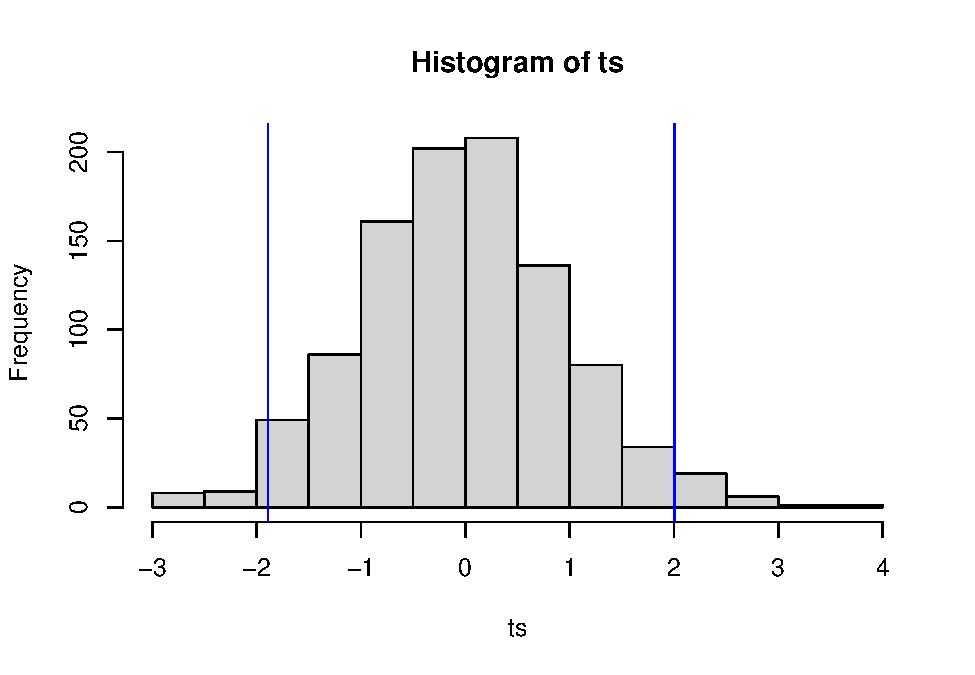
\includegraphics{03-RandomizationTests_files/figure-latex/unnamed-chunk-4-1.pdf}

The \(t_0\) value of \(-5.83\) is off the chart (literally). How do we interpret this? The test randomly labels observed sexes with observed salaries. The observed test statistic suggests this is not how the salaries were actually assigned to workers. That's pretty obvious---companies do not tend to assign salaries in a random fashion. But, if the salary assignment was not random with respect to sex, then it either depended on sex or depends on a hidden variable closely associated with sex. Since the job, time frame, and experience level were controlled for, it is certainly plausible that the salary assignment depended on sex.

\begin{Shaded}
\begin{Highlighting}[]
\NormalTok{n0 }\OtherTok{\textless{}{-}} \FunctionTok{sum}\NormalTok{(salaries.df}\SpecialCharTok{$}\NormalTok{Sex}\SpecialCharTok{==}\DecValTok{0}\NormalTok{)}
\NormalTok{n1 }\OtherTok{\textless{}{-}} \FunctionTok{sum}\NormalTok{(salaries.df}\SpecialCharTok{$}\NormalTok{Sex}\SpecialCharTok{==}\DecValTok{1}\NormalTok{)}
\NormalTok{n }\OtherTok{\textless{}{-}}\NormalTok{ n0}\SpecialCharTok{+}\NormalTok{n1}
\NormalTok{randomization.test }\OtherTok{\textless{}{-}} \ControlFlowTok{function}\NormalTok{(M, df)\{}
\NormalTok{  ts }\OtherTok{\textless{}{-}} \FunctionTok{rep}\NormalTok{(}\ConstantTok{NA}\NormalTok{,M)}
  \ControlFlowTok{for}\NormalTok{(m }\ControlFlowTok{in} \DecValTok{1}\SpecialCharTok{:}\NormalTok{M)\{}
\NormalTok{    permute.n }\OtherTok{\textless{}{-}} \FunctionTok{sample.int}\NormalTok{(n,n,}\AttributeTok{replace =}\NormalTok{ F)}
\NormalTok{    re.randomized.group }\OtherTok{\textless{}{-}}\NormalTok{ df}\SpecialCharTok{$}\NormalTok{Sex[permute.n]}
\NormalTok{    m0 }\OtherTok{\textless{}{-}} \FunctionTok{mean}\NormalTok{(df}\SpecialCharTok{$}\NormalTok{Salary[re.randomized.group}\SpecialCharTok{==}\DecValTok{0}\NormalTok{])}
\NormalTok{    m1 }\OtherTok{\textless{}{-}} \FunctionTok{mean}\NormalTok{(df}\SpecialCharTok{$}\NormalTok{Salary[re.randomized.group}\SpecialCharTok{==}\DecValTok{1}\NormalTok{])}
\NormalTok{    s0 }\OtherTok{\textless{}{-}} \FunctionTok{var}\NormalTok{(df}\SpecialCharTok{$}\NormalTok{Salary[re.randomized.group}\SpecialCharTok{==}\DecValTok{0}\NormalTok{])}
\NormalTok{    s1 }\OtherTok{\textless{}{-}} \FunctionTok{var}\NormalTok{(df}\SpecialCharTok{$}\NormalTok{Salary[re.randomized.group}\SpecialCharTok{==}\DecValTok{1}\NormalTok{])}
\NormalTok{    ts[m] }\OtherTok{\textless{}{-}}\NormalTok{ (m0 }\SpecialCharTok{{-}}\NormalTok{ m1)}\SpecialCharTok{/}\FunctionTok{sqrt}\NormalTok{(s0}\SpecialCharTok{/}\NormalTok{n0}\SpecialCharTok{+}\NormalTok{s1}\SpecialCharTok{/}\NormalTok{n1)}
\NormalTok{    \}}
  \FunctionTok{return}\NormalTok{(ts)}
\NormalTok{\}}


\NormalTok{grid.delta }\OtherTok{\textless{}{-}} \FunctionTok{seq}\NormalTok{(}\AttributeTok{from =} \DecValTok{400}\NormalTok{, }\AttributeTok{to =} \DecValTok{1400}\NormalTok{, }\AttributeTok{length.out =} \DecValTok{100}\NormalTok{)}
\NormalTok{L }\OtherTok{\textless{}{-}} \FunctionTok{length}\NormalTok{(grid.delta)}
\NormalTok{p.value }\OtherTok{\textless{}{-}} \FunctionTok{rep}\NormalTok{(}\ConstantTok{NA}\NormalTok{,L)}
\NormalTok{reject}\OtherTok{\textless{}{-}}\FunctionTok{rep}\NormalTok{(}\ConstantTok{NA}\NormalTok{, L)            }
\ControlFlowTok{for}\NormalTok{(j }\ControlFlowTok{in} \DecValTok{1}\SpecialCharTok{:}\NormalTok{L)\{}
\NormalTok{temp.df }\OtherTok{\textless{}{-}}\NormalTok{ salaries.df}
\NormalTok{temp.df}\SpecialCharTok{$}\NormalTok{Salary[temp.df}\SpecialCharTok{$}\NormalTok{Sex}\SpecialCharTok{==}\DecValTok{1}\NormalTok{]}\OtherTok{\textless{}{-}}\NormalTok{temp.df}\SpecialCharTok{$}\NormalTok{Salary[temp.df}\SpecialCharTok{$}\NormalTok{Sex}\SpecialCharTok{==}\DecValTok{1}\NormalTok{]}\SpecialCharTok{{-}}\NormalTok{grid.delta[j]}
\NormalTok{m0 }\OtherTok{\textless{}{-}} \FunctionTok{mean}\NormalTok{(temp.df}\SpecialCharTok{$}\NormalTok{Salary[temp.df}\SpecialCharTok{$}\NormalTok{Sex}\SpecialCharTok{==}\DecValTok{0}\NormalTok{])}
\NormalTok{m1 }\OtherTok{\textless{}{-}} \FunctionTok{mean}\NormalTok{(temp.df}\SpecialCharTok{$}\NormalTok{Salary[temp.df}\SpecialCharTok{$}\NormalTok{Sex}\SpecialCharTok{==}\DecValTok{1}\NormalTok{])}
\NormalTok{s0 }\OtherTok{\textless{}{-}} \FunctionTok{var}\NormalTok{(temp.df}\SpecialCharTok{$}\NormalTok{Salary[temp.df}\SpecialCharTok{$}\NormalTok{Sex}\SpecialCharTok{==}\DecValTok{0}\NormalTok{])}
\NormalTok{s1 }\OtherTok{\textless{}{-}} \FunctionTok{var}\NormalTok{(temp.df}\SpecialCharTok{$}\NormalTok{Salary[temp.df}\SpecialCharTok{$}\NormalTok{Sex}\SpecialCharTok{==}\DecValTok{1}\NormalTok{])}
\NormalTok{t0 }\OtherTok{\textless{}{-}}\NormalTok{ (m0 }\SpecialCharTok{{-}}\NormalTok{ m1)}\SpecialCharTok{/}\FunctionTok{sqrt}\NormalTok{(s0}\SpecialCharTok{/}\NormalTok{n0}\SpecialCharTok{+}\NormalTok{s1}\SpecialCharTok{/}\NormalTok{n1)}
\NormalTok{test.vals.j }\OtherTok{\textless{}{-}} \FunctionTok{randomization.test}\NormalTok{(}\DecValTok{10000}\NormalTok{, temp.df)}
\NormalTok{mean.randomization }\OtherTok{\textless{}{-}} \FunctionTok{mean}\NormalTok{(test.vals.j)}
\NormalTok{p.value[j] }\OtherTok{\textless{}{-}} \FunctionTok{ifelse}\NormalTok{(t0 }\SpecialCharTok{\textgreater{}}\NormalTok{ mean.randomization,}\FunctionTok{sum}\NormalTok{(}\FunctionTok{abs}\NormalTok{(test.vals.j)}\SpecialCharTok{\textgreater{}}\NormalTok{t0)}\SpecialCharTok{/}\DecValTok{10000}\NormalTok{,}\FunctionTok{sum}\NormalTok{(}\SpecialCharTok{{-}}\FunctionTok{abs}\NormalTok{(test.vals.j)}\SpecialCharTok{\textless{}}\NormalTok{t0)}\SpecialCharTok{/}\DecValTok{10000}\NormalTok{)}
\NormalTok{\}}
\FunctionTok{cbind}\NormalTok{(grid.delta, p.value)}
\end{Highlighting}
\end{Shaded}

\begin{verbatim}
##        grid.delta p.value
##   [1,]   400.0000  0.0038
##   [2,]   410.1010  0.0040
##   [3,]   420.2020  0.0068
##   [4,]   430.3030  0.0078
##   [5,]   440.4040  0.0079
##   [6,]   450.5051  0.0106
##   [7,]   460.6061  0.0123
##   [8,]   470.7071  0.0142
##   [9,]   480.8081  0.0170
##  [10,]   490.9091  0.0188
##  [11,]   501.0101  0.0276
##  [12,]   511.1111  0.0317
##  [13,]   521.2121  0.0374
##  [14,]   531.3131  0.0415
##  [15,]   541.4141  0.0496
##  [16,]   551.5152  0.0598
##  [17,]   561.6162  0.0727
##  [18,]   571.7172  0.0823
##  [19,]   581.8182  0.0952
##  [20,]   591.9192  0.1132
##  [21,]   602.0202  0.1295
##  [22,]   612.1212  0.1484
##  [23,]   622.2222  0.1698
##  [24,]   632.3232  0.1932
##  [25,]   642.4242  0.2116
##  [26,]   652.5253  0.2535
##  [27,]   662.6263  0.2700
##  [28,]   672.7273  0.3006
##  [29,]   682.8283  0.3385
##  [30,]   692.9293  0.3814
##  [31,]   703.0303  0.4210
##  [32,]   713.1313  0.4567
##  [33,]   723.2323  0.5046
##  [34,]   733.3333  0.5444
##  [35,]   743.4343  0.6021
##  [36,]   753.5354  0.6418
##  [37,]   763.6364  0.7020
##  [38,]   773.7374  0.7513
##  [39,]   783.8384  0.8085
##  [40,]   793.9394  0.8648
##  [41,]   804.0404  0.9259
##  [42,]   814.1414  0.9766
##  [43,]   824.2424  0.9690
##  [44,]   834.3434  0.9066
##  [45,]   844.4444  0.8595
##  [46,]   854.5455  0.7955
##  [47,]   864.6465  0.7354
##  [48,]   874.7475  0.6922
##  [49,]   884.8485  0.6391
##  [50,]   894.9495  0.5835
##  [51,]   905.0505  0.5432
##  [52,]   915.1515  0.4895
##  [53,]   925.2525  0.4505
##  [54,]   935.3535  0.4126
##  [55,]   945.4545  0.3676
##  [56,]   955.5556  0.3285
##  [57,]   965.6566  0.2918
##  [58,]   975.7576  0.2609
##  [59,]   985.8586  0.2415
##  [60,]   995.9596  0.2065
##  [61,]  1006.0606  0.1829
##  [62,]  1016.1616  0.1658
##  [63,]  1026.2626  0.1415
##  [64,]  1036.3636  0.1237
##  [65,]  1046.4646  0.1110
##  [66,]  1056.5657  0.0925
##  [67,]  1066.6667  0.0838
##  [68,]  1076.7677  0.0673
##  [69,]  1086.8687  0.0598
##  [70,]  1096.9697  0.0507
##  [71,]  1107.0707  0.0433
##  [72,]  1117.1717  0.0384
##  [73,]  1127.2727  0.0308
##  [74,]  1137.3737  0.0267
##  [75,]  1147.4747  0.0229
##  [76,]  1157.5758  0.0191
##  [77,]  1167.6768  0.0167
##  [78,]  1177.7778  0.0117
##  [79,]  1187.8788  0.0097
##  [80,]  1197.9798  0.0082
##  [81,]  1208.0808  0.0073
##  [82,]  1218.1818  0.0070
##  [83,]  1228.2828  0.0047
##  [84,]  1238.3838  0.0036
##  [85,]  1248.4848  0.0038
##  [86,]  1258.5859  0.0026
##  [87,]  1268.6869  0.0017
##  [88,]  1278.7879  0.0016
##  [89,]  1288.8889  0.0010
##  [90,]  1298.9899  0.0011
##  [91,]  1309.0909  0.0013
##  [92,]  1319.1919  0.0004
##  [93,]  1329.2929  0.0004
##  [94,]  1339.3939  0.0005
##  [95,]  1349.4949  0.0005
##  [96,]  1359.5960  0.0003
##  [97,]  1369.6970  0.0001
##  [98,]  1379.7980  0.0002
##  [99,]  1389.8990  0.0001
## [100,]  1400.0000  0.0001
\end{verbatim}

\begin{Shaded}
\begin{Highlighting}[]
\NormalTok{midpoint }\OtherTok{\textless{}{-}} \FunctionTok{which.max}\NormalTok{(p.value)}
\NormalTok{lower.endpoint }\OtherTok{\textless{}{-}}\NormalTok{ grid.delta[}\FunctionTok{which.min}\NormalTok{(}\FunctionTok{abs}\NormalTok{(}\FloatTok{0.05}\SpecialCharTok{{-}}\NormalTok{p.value[}\DecValTok{1}\SpecialCharTok{:}\NormalTok{midpoint]))]}
\NormalTok{upper.endpoint }\OtherTok{\textless{}{-}}\NormalTok{ grid.delta[midpoint}\SpecialCharTok{+}\FunctionTok{which.min}\NormalTok{(}\FunctionTok{abs}\NormalTok{(}\FloatTok{0.05}\SpecialCharTok{{-}}\NormalTok{p.value[(midpoint}\SpecialCharTok{+}\DecValTok{1}\NormalTok{)}\SpecialCharTok{:}\NormalTok{L]))]}
\FunctionTok{c}\NormalTok{(lower.endpoint, upper.endpoint)}
\end{Highlighting}
\end{Shaded}

\begin{verbatim}
## [1]  541.4141 1096.9697
\end{verbatim}

\hypertarget{alternatives-for-non-normal-responses}{%
\chapter{Alternatives for Non-Normal Responses}\label{alternatives-for-non-normal-responses}}

When responses (or residuals) appear non-normal we may doubt the validity of z-, t-, and F- tests, especially for small sample sizes. We'll discuss two strategies for dealing with non-normality: transformations and robust tests.

\hypertarget{transformations}{%
\section{Transformations}\label{transformations}}

Sometimes, when residuals/responses appear non-normal, a particular transformation/function of the values will produce residuals/responses that do appear normal. The case-in-point is the Lognormal distribution. It is, essentially, defined by the following relationship: If \(X\sim\)Lognormal, then \(\log(X)\sim\)Normal. And, vice-versa, if \(Y\sim\)Normal, then \(\exp(Y)\sim\)Lognormal. A random sample from a lognormal distribution will appear skewed to the right, or positively skewed. The log transformation dampens large (absolute) values more than small ones, reducing or removing the skew.

\begin{Shaded}
\begin{Highlighting}[]
\NormalTok{Y }\OtherTok{\textless{}{-}} \FunctionTok{exp}\NormalTok{(}\FunctionTok{rnorm}\NormalTok{(}\DecValTok{101}\NormalTok{))}
\FunctionTok{par}\NormalTok{(}\AttributeTok{mfrow =} \FunctionTok{c}\NormalTok{(}\DecValTok{1}\NormalTok{,}\DecValTok{2}\NormalTok{))}
\FunctionTok{hist}\NormalTok{(Y, }\AttributeTok{main =} \StringTok{\textquotesingle{}A random sample of 101 Lognormal r.v. s\textquotesingle{}}\NormalTok{)}
\FunctionTok{hist}\NormalTok{(}\FunctionTok{log}\NormalTok{(Y), }\AttributeTok{main =} \StringTok{\textquotesingle{}Same data after log{-}transform\textquotesingle{}}\NormalTok{)}
\end{Highlighting}
\end{Shaded}

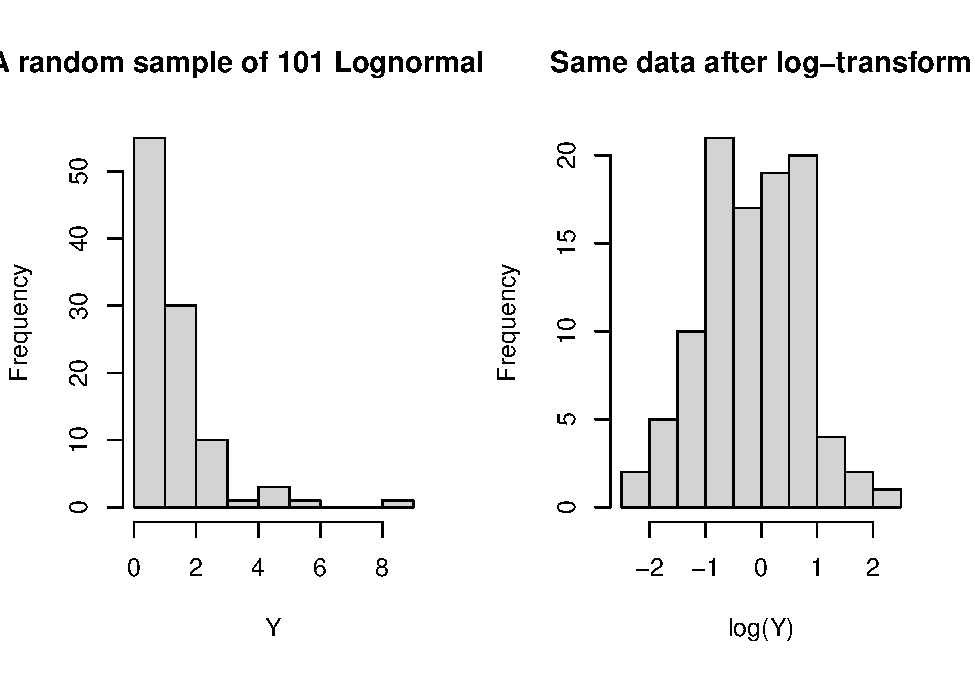
\includegraphics{04-Non-Normal-Responses_files/figure-latex/unnamed-chunk-1-1.pdf}

\begin{Shaded}
\begin{Highlighting}[]
\FunctionTok{median}\NormalTok{(Y)}
\end{Highlighting}
\end{Shaded}

\begin{verbatim}
## [1] 1.037574
\end{verbatim}

\begin{Shaded}
\begin{Highlighting}[]
\FunctionTok{median}\NormalTok{(}\FunctionTok{log}\NormalTok{(Y))}
\end{Highlighting}
\end{Shaded}

\begin{verbatim}
## [1] 0.03688552
\end{verbatim}

\begin{Shaded}
\begin{Highlighting}[]
\FunctionTok{log}\NormalTok{(}\FunctionTok{median}\NormalTok{(Y))}
\end{Highlighting}
\end{Shaded}

\begin{verbatim}
## [1] 0.03688552
\end{verbatim}

Of course, the log-transform can only be applied to positive data values, and is meant specifically for use with positively skewed data. Since the log transform is monotonic increasing it preserves medians. That is, the median of the log-transformed values is equal to the log of the median of the original values. This is helpful for interpreting the results of tests concerning the mean of the log-transformed values.

Allow me to elaborate. Consider a one-sample test of \(H_0:\mu = \mu_0\) where \(\mu\) denotes the population mean of the log-transformed random variable \(X = \log(Y)\). Assuming \(X\) follows a normal distribution, its mean and median are the same. So, if we reject the hypothesis and say \(\mu \ne \mu_0\) this is equivalent to saying the \textbf{median} of the \(Y\) population is not \(\log(\mu_0)\).

For a two sample test of \(H_0:\mu_1 = \mu_2\) the point estimate \(\overline X_1 - \overline X_2\) measures the difference in population means for the log-transformed random variables, and \(\exp(\overline X_1 - \overline X_2)\) estimates the \textbf{ratio of medians} for the populations on the original scale.

The log transform is not the only transformation that may aid in ``normalizing'' right-skewed responses. Sometimes a square root transformation is appropriate. A general method is available to select the ``best'' normalizing transformation for right-skewed data. I won't elaborate on this method here, but simply note that in R the function ``boxcox'' will determine a good transformation to use to normalize right-skewed responses. These transformations are the Box-Cox family of functions
\[\frac{y^\gamma - 1}{\gamma}\quad \gamma \ne 0, \]
and where the transformation is defined to be the log-transform when \(\gamma = 0\).

\hypertarget{example-cloud-seeding-for-rainfall}{%
\subsection{Example: Cloud Seeding for Rainfall}\label{example-cloud-seeding-for-rainfall}}

The data frame ``clouds'' in the HSAUR2 package contains rainfall measurements (among other things) when researchers have ``seeded'' clouds in the atmosphere compared to when they have not done so. The data is noticeably right-skewed, and, of course positive because we're talking about rainfall measurments.

\begin{Shaded}
\begin{Highlighting}[]
\FunctionTok{library}\NormalTok{(HSAUR2)}
\end{Highlighting}
\end{Shaded}

\begin{verbatim}
## Loading required package: tools
\end{verbatim}

\begin{Shaded}
\begin{Highlighting}[]
\FunctionTok{boxplot}\NormalTok{(rainfall }\SpecialCharTok{\textasciitilde{}}\NormalTok{ seeding, }\AttributeTok{data =}\NormalTok{ clouds, }\AttributeTok{ylab =} \StringTok{"Rainfall"}\NormalTok{)}
\end{Highlighting}
\end{Shaded}

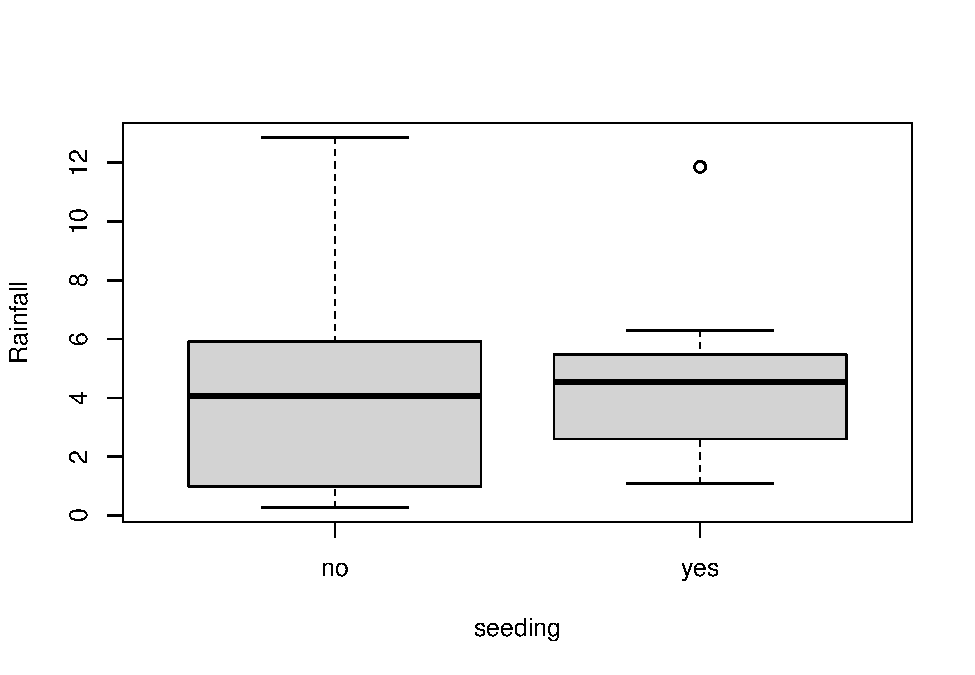
\includegraphics{04-Non-Normal-Responses_files/figure-latex/unnamed-chunk-2-1.pdf}

Using the boxcox function we see that the ``best'' normalizing transformation has \(\gamma \approx 0.42\). Briefly, the ``best'' transformation is the one maximizing a normal likelihood. And, indeed boxplots of rainfall measurements under this transformation appear closer to normal.

\begin{Shaded}
\begin{Highlighting}[]
\FunctionTok{library}\NormalTok{(MASS)}
\NormalTok{bc }\OtherTok{\textless{}{-}} \FunctionTok{boxcox}\NormalTok{(rainfall}\SpecialCharTok{\textasciitilde{}}\NormalTok{seeding, }\AttributeTok{data =}\NormalTok{ clouds)}
\end{Highlighting}
\end{Shaded}

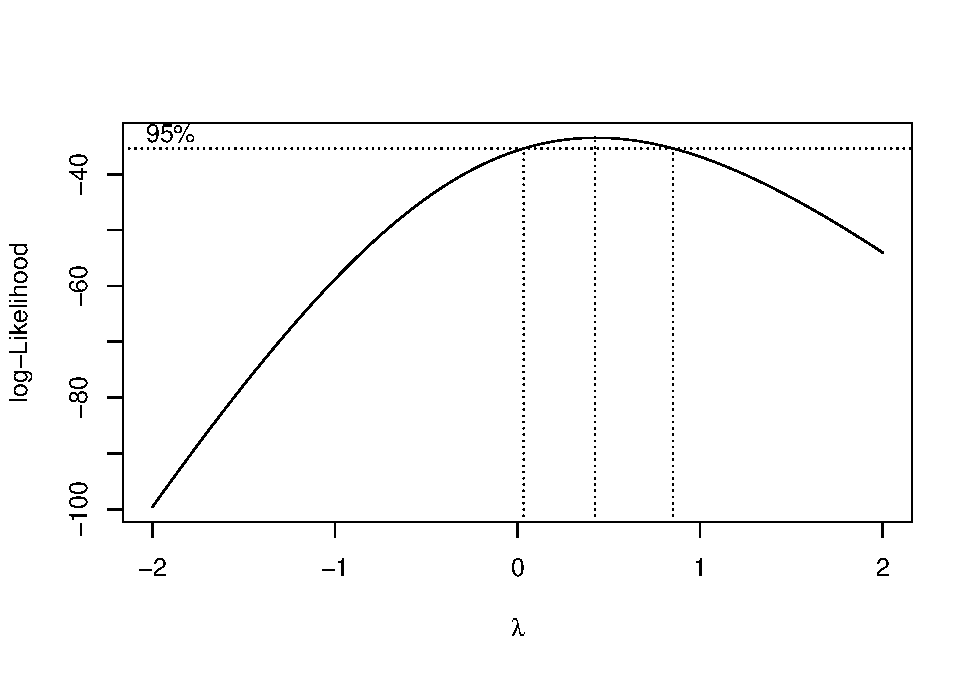
\includegraphics{04-Non-Normal-Responses_files/figure-latex/unnamed-chunk-3-1.pdf}

\begin{Shaded}
\begin{Highlighting}[]
\NormalTok{bc}\SpecialCharTok{$}\NormalTok{x[}\FunctionTok{which.max}\NormalTok{(bc}\SpecialCharTok{$}\NormalTok{y)]}
\end{Highlighting}
\end{Shaded}

\begin{verbatim}
## [1] 0.4242424
\end{verbatim}

\begin{Shaded}
\begin{Highlighting}[]
\NormalTok{my.clouds }\OtherTok{\textless{}{-}}\NormalTok{ clouds}
\NormalTok{my.clouds}\SpecialCharTok{$}\NormalTok{bc }\OtherTok{\textless{}{-}}\NormalTok{ (my.clouds}\SpecialCharTok{$}\NormalTok{rainfall}\SpecialCharTok{\^{}}\FloatTok{0.42} \SpecialCharTok{{-}} \DecValTok{1}\NormalTok{)}\SpecialCharTok{/} \FloatTok{0.42}
\FunctionTok{boxplot}\NormalTok{(bc}\SpecialCharTok{\textasciitilde{}}\NormalTok{seeding, }\AttributeTok{data =}\NormalTok{ my.clouds)}
\end{Highlighting}
\end{Shaded}

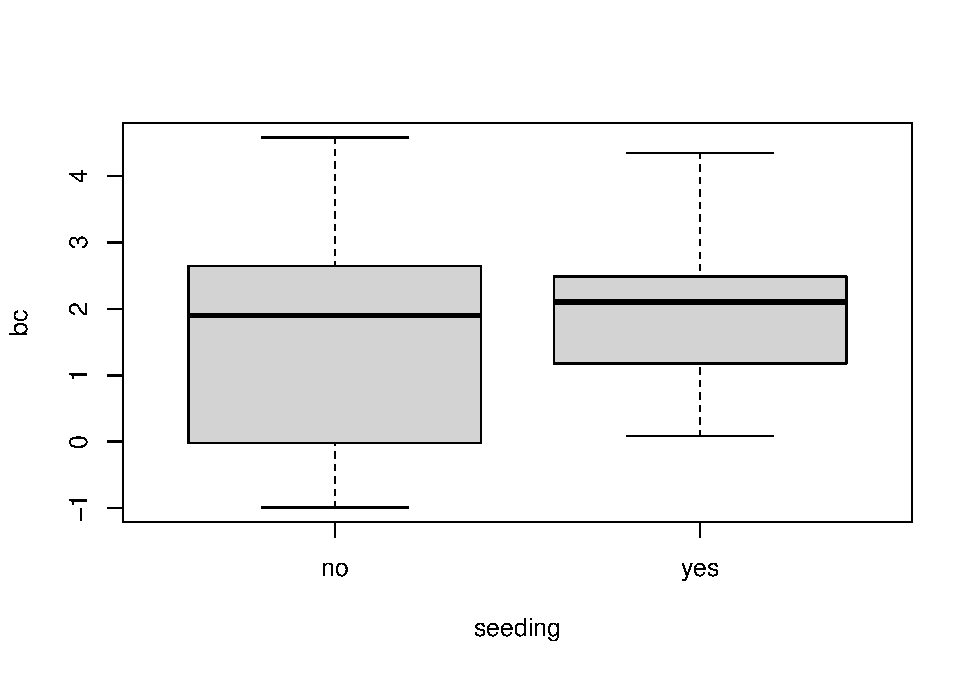
\includegraphics{04-Non-Normal-Responses_files/figure-latex/unnamed-chunk-3-2.pdf}

Let's do a two-sample t-test for difference in mean rainfall under seeding/non-seeding conditions. Remember to interpret the results carefully due to our transformation.

\begin{Shaded}
\begin{Highlighting}[]
\NormalTok{bc.t.test }\OtherTok{\textless{}{-}} \FunctionTok{t.test}\NormalTok{(my.clouds}\SpecialCharTok{$}\NormalTok{bc[my.clouds}\SpecialCharTok{$}\NormalTok{seeding }\SpecialCharTok{==} \StringTok{\textquotesingle{}no\textquotesingle{}}\NormalTok{], my.clouds}\SpecialCharTok{$}\NormalTok{bc[my.clouds}\SpecialCharTok{$}\NormalTok{seeding }\SpecialCharTok{==} \StringTok{\textquotesingle{}yes\textquotesingle{}}\NormalTok{], }\AttributeTok{alternative =} \StringTok{\textquotesingle{}two.sided\textquotesingle{}}\NormalTok{)}
\NormalTok{bc.t.test}
\end{Highlighting}
\end{Shaded}

\begin{verbatim}
## 
##  Welch Two Sample t-test
## 
## data:  my.clouds$bc[my.clouds$seeding == "no"] and my.clouds$bc[my.clouds$seeding == "yes"]
## t = -0.7541, df = 19.094, p-value = 0.46
## alternative hypothesis: true difference in means is not equal to 0
## 95 percent confidence interval:
##  -1.6280579  0.7654181
## sample estimates:
## mean of x mean of y 
##  1.551329  1.982649
\end{verbatim}

\begin{Shaded}
\begin{Highlighting}[]
\NormalTok{n1 }\OtherTok{\textless{}{-}} \FunctionTok{sum}\NormalTok{(my.clouds}\SpecialCharTok{$}\NormalTok{seeding }\SpecialCharTok{==} \StringTok{\textquotesingle{}no\textquotesingle{}}\NormalTok{)}
\NormalTok{n2 }\OtherTok{\textless{}{-}} \FunctionTok{sum}\NormalTok{(my.clouds}\SpecialCharTok{$}\NormalTok{seeding }\SpecialCharTok{==} \StringTok{\textquotesingle{}yes\textquotesingle{}}\NormalTok{)}
\NormalTok{sp2 }\OtherTok{\textless{}{-}}\NormalTok{ (n1}\SpecialCharTok{*}\FunctionTok{var}\NormalTok{(my.clouds}\SpecialCharTok{$}\NormalTok{bc[my.clouds}\SpecialCharTok{$}\NormalTok{seeding }\SpecialCharTok{==} \StringTok{\textquotesingle{}no\textquotesingle{}}\NormalTok{]) }\SpecialCharTok{+}\NormalTok{ n2}\SpecialCharTok{*}\FunctionTok{var}\NormalTok{(my.clouds}\SpecialCharTok{$}\NormalTok{bc[my.clouds}\SpecialCharTok{$}\NormalTok{seeding }\SpecialCharTok{==} \StringTok{\textquotesingle{}yes\textquotesingle{}}\NormalTok{]))}\SpecialCharTok{/}\NormalTok{(n1}\SpecialCharTok{+}\NormalTok{n2}\DecValTok{{-}2}\NormalTok{)}
\NormalTok{residuals }\OtherTok{\textless{}{-}} \FunctionTok{c}\NormalTok{( my.clouds}\SpecialCharTok{$}\NormalTok{bc[my.clouds}\SpecialCharTok{$}\NormalTok{seeding }\SpecialCharTok{==} \StringTok{\textquotesingle{}no\textquotesingle{}}\NormalTok{] }\SpecialCharTok{{-}} \FunctionTok{mean}\NormalTok{(my.clouds}\SpecialCharTok{$}\NormalTok{bc[my.clouds}\SpecialCharTok{$}\NormalTok{seeding }\SpecialCharTok{==} \StringTok{\textquotesingle{}no\textquotesingle{}}\NormalTok{]), my.clouds}\SpecialCharTok{$}\NormalTok{bc[my.clouds}\SpecialCharTok{$}\NormalTok{seeding }\SpecialCharTok{==} \StringTok{\textquotesingle{}yes\textquotesingle{}}\NormalTok{] }\SpecialCharTok{{-}} \FunctionTok{mean}\NormalTok{(my.clouds}\SpecialCharTok{$}\NormalTok{bc[my.clouds}\SpecialCharTok{$}\NormalTok{seeding }\SpecialCharTok{==} \StringTok{\textquotesingle{}yes\textquotesingle{}}\NormalTok{])  )}\SpecialCharTok{/}\FunctionTok{sqrt}\NormalTok{(sp2)}
\FunctionTok{qqnorm}\NormalTok{(residuals)}
\FunctionTok{qqline}\NormalTok{(residuals)}
\end{Highlighting}
\end{Shaded}

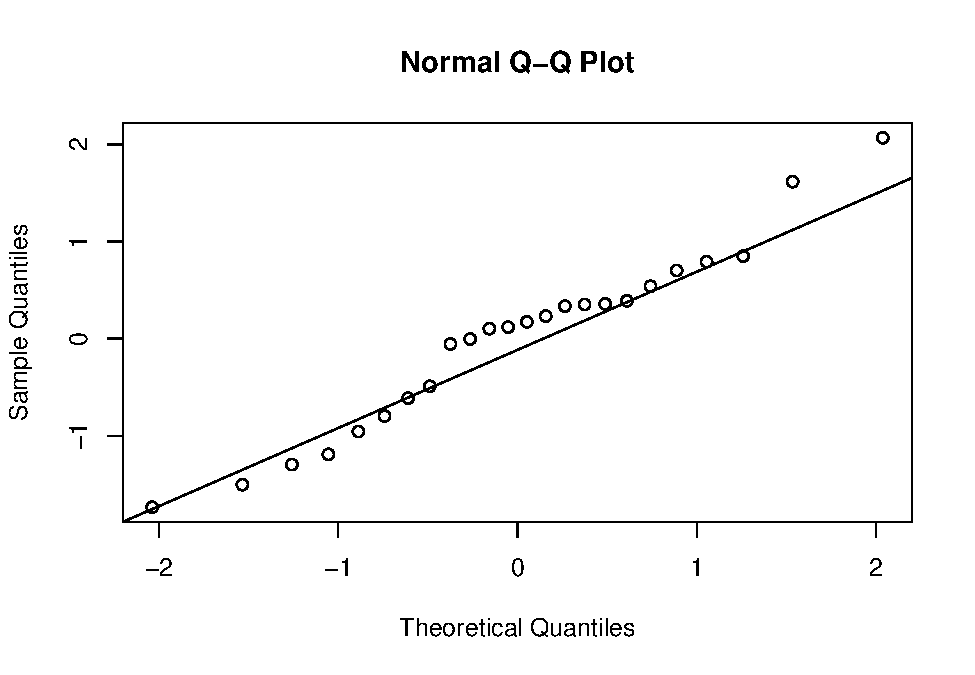
\includegraphics{04-Non-Normal-Responses_files/figure-latex/unnamed-chunk-4-1.pdf}

We do not reject the hypothesis of equal mean (transformed) rainfall. On the original data scale, we say the ratio of population median rainfall amounts is not significantly different than 1.

We can look also at the t-test on the original data scale and see to what extent the residuals may suggest the normality assumption is suspect.

\begin{Shaded}
\begin{Highlighting}[]
\NormalTok{orig.t.test }\OtherTok{\textless{}{-}} \FunctionTok{t.test}\NormalTok{(clouds}\SpecialCharTok{$}\NormalTok{rainfall[my.clouds}\SpecialCharTok{$}\NormalTok{seeding }\SpecialCharTok{==} \StringTok{\textquotesingle{}no\textquotesingle{}}\NormalTok{], clouds}\SpecialCharTok{$}\NormalTok{rainfall[clouds}\SpecialCharTok{$}\NormalTok{seeding }\SpecialCharTok{==} \StringTok{\textquotesingle{}yes\textquotesingle{}}\NormalTok{], }\AttributeTok{alternative =} \StringTok{\textquotesingle{}two.sided\textquotesingle{}}\NormalTok{)}
\NormalTok{orig.t.test}
\end{Highlighting}
\end{Shaded}

\begin{verbatim}
## 
##  Welch Two Sample t-test
## 
## data:  clouds$rainfall[my.clouds$seeding == "no"] and clouds$rainfall[clouds$seeding == "yes"]
## t = -0.3574, df = 20.871, p-value = 0.7244
## alternative hypothesis: true difference in means is not equal to 0
## 95 percent confidence interval:
##  -3.154691  2.229691
## sample estimates:
## mean of x mean of y 
##  4.171667  4.634167
\end{verbatim}

\begin{Shaded}
\begin{Highlighting}[]
\NormalTok{n1 }\OtherTok{\textless{}{-}} \FunctionTok{sum}\NormalTok{(clouds}\SpecialCharTok{$}\NormalTok{seeding }\SpecialCharTok{==} \StringTok{\textquotesingle{}no\textquotesingle{}}\NormalTok{)}
\NormalTok{n2 }\OtherTok{\textless{}{-}} \FunctionTok{sum}\NormalTok{(clouds}\SpecialCharTok{$}\NormalTok{seeding }\SpecialCharTok{==} \StringTok{\textquotesingle{}yes\textquotesingle{}}\NormalTok{)}
\NormalTok{sp2 }\OtherTok{\textless{}{-}}\NormalTok{ (n1}\SpecialCharTok{*}\FunctionTok{var}\NormalTok{(clouds}\SpecialCharTok{$}\NormalTok{rainfall[clouds}\SpecialCharTok{$}\NormalTok{seeding }\SpecialCharTok{==} \StringTok{\textquotesingle{}no\textquotesingle{}}\NormalTok{]) }\SpecialCharTok{+}\NormalTok{ n2}\SpecialCharTok{*}\FunctionTok{var}\NormalTok{(clouds}\SpecialCharTok{$}\NormalTok{rainfall[clouds}\SpecialCharTok{$}\NormalTok{seeding }\SpecialCharTok{==} \StringTok{\textquotesingle{}yes\textquotesingle{}}\NormalTok{]))}\SpecialCharTok{/}\NormalTok{(n1}\SpecialCharTok{+}\NormalTok{n2}\DecValTok{{-}2}\NormalTok{)}
\NormalTok{residuals }\OtherTok{\textless{}{-}} \FunctionTok{c}\NormalTok{( clouds}\SpecialCharTok{$}\NormalTok{rainfall[clouds}\SpecialCharTok{$}\NormalTok{seeding }\SpecialCharTok{==} \StringTok{\textquotesingle{}no\textquotesingle{}}\NormalTok{] }\SpecialCharTok{{-}} \FunctionTok{mean}\NormalTok{(clouds}\SpecialCharTok{$}\NormalTok{rainfall[clouds}\SpecialCharTok{$}\NormalTok{seeding }\SpecialCharTok{==} \StringTok{\textquotesingle{}no\textquotesingle{}}\NormalTok{]), clouds}\SpecialCharTok{$}\NormalTok{rainfall[clouds}\SpecialCharTok{$}\NormalTok{seeding }\SpecialCharTok{==} \StringTok{\textquotesingle{}yes\textquotesingle{}}\NormalTok{] }\SpecialCharTok{{-}} \FunctionTok{mean}\NormalTok{(clouds}\SpecialCharTok{$}\NormalTok{rainfall[clouds}\SpecialCharTok{$}\NormalTok{seeding }\SpecialCharTok{==} \StringTok{\textquotesingle{}yes\textquotesingle{}}\NormalTok{])  )}\SpecialCharTok{/}\FunctionTok{sqrt}\NormalTok{(sp2)}
\FunctionTok{qqnorm}\NormalTok{(residuals)}
\FunctionTok{qqline}\NormalTok{(residuals)}
\end{Highlighting}
\end{Shaded}

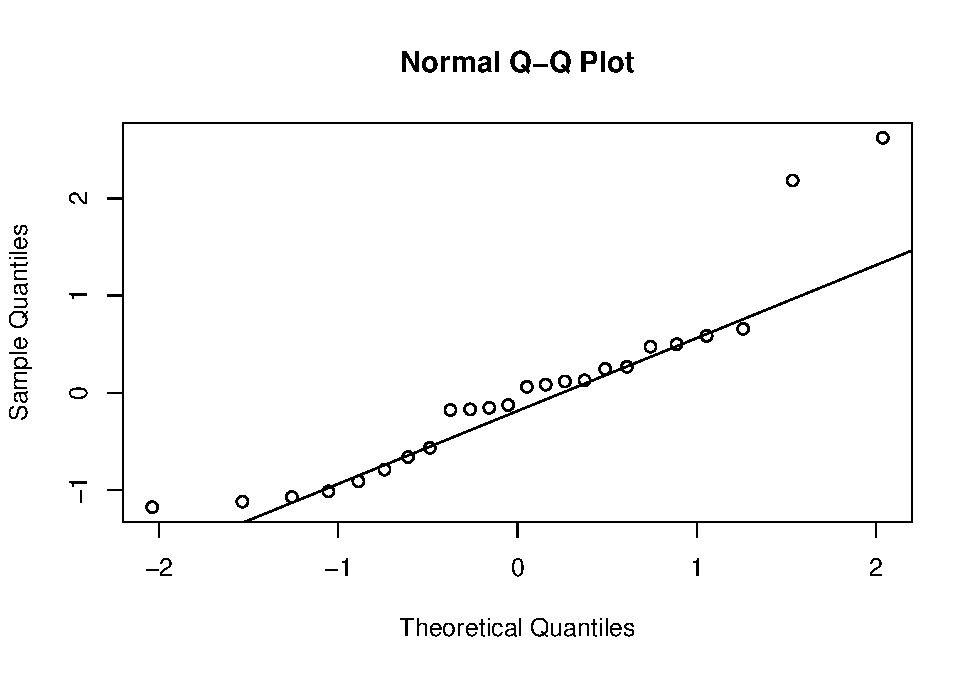
\includegraphics{04-Non-Normal-Responses_files/figure-latex/unnamed-chunk-5-1.pdf}

At least the tails of the residuals certainly look like less of a match than the Box-Cox transformed responses. This is consistent with the strong right skew we see in the original rainfall data.

\hypertarget{rank-sum-test}{%
\section{Rank-Sum Test}\label{rank-sum-test}}

We have seen that certain one-to-one transformations can be helpful when dealing with positively-skewed responses. But, what about other types of non-normal data? One general-purpose approach to comparing two populations of non-normal responses is to apply a rank transformation and use the Mann-Whitney (Rank-Sum) test.

Unlike the previous Box-Cox transformations, the rank transformation is not one-to-one, so some information is lost moving from the original to the transformed data (the ranks). But, in exchange for this price we pay we obtain a data set that is easier to analyze, especially in certain special cases.

To perform the rank-sum test we first sort all the responses, with the two groups pooled together. If some responses have the same value, we assign to them the average of the corresponding ranks. For example, the sorted responses 1,2,2,3,4,6 would get the ranks 1,2.5,2.5,4,5,6. Let \(T = \max\{T_1, T_2\}\) where \(T_1\) and \(T_2\) are the sums of the ranks for responses in groups 1 and 2, respectively. Let \(n_T\) be the sample size of the group corresponding to \(T\). Let \(\overline r\) and \(s_r\) be the sample mean and sample standard deviation of all of the ranks. Then, the rank-sum test statistic is defined as
\[z = \frac{T - n_T\overline r}{s_r\sqrt{\frac{n_1n_2}{n_1+n_2}}}.\]
For large \(n_1\) and \(n_2\), \(z \stackrel{\cdot}{\sim}N(0,1)\), so the test conclusion follows from comparing \(z\) to standard normal quantiles. For example, the p-value is \(2(1-\Phi(z))\).

Just what does the rank-sum test test? In the most general form, under no further assumptions, the rank-sum tests equality of distributions of the response in the two groups. However, the test will only detect differences in those distributions if \(P(X_1 > X_2) \ne P(X_2 > X_1)\) where \(X_1\) and \(x_2\) denote the response random variable from each population. For example, if the populations are both normal with the same mean but different variances, then the rank-sum test will not generally be able to distinguish between the populations. In the special case that the populations are different by a location shift, i.e., \(F_1(x) = F_1(x+c)\) for a constant \(c\), the null hypothesis is equivalent to testing equality of population medians.

\hypertarget{example-ratio-measurements}{%
\subsection{Example: ratio measurements}\label{example-ratio-measurements}}

The following data represent the ratios of lengths of canine and molar teeth in two populations of animals: wild and captive. Ratios are tricky, and may behave badly when the denominator can be close to zero. These ratio measurements exhibit non-normality, but not positive skew like we have seen before.

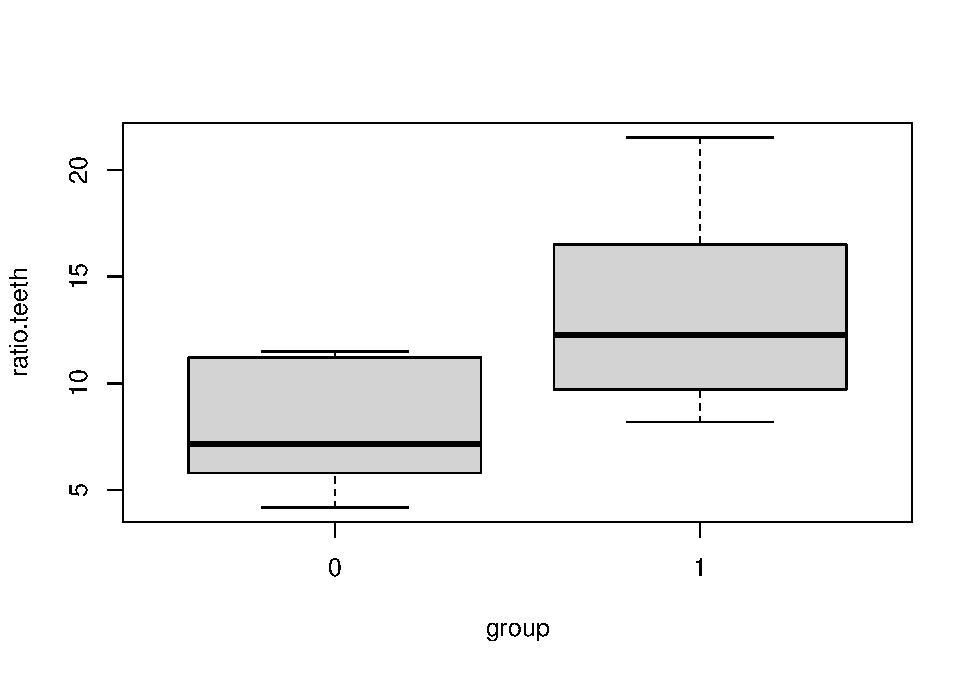
\includegraphics{04-Non-Normal-Responses_files/figure-latex/unnamed-chunk-7-1.pdf}

Next, we'll implement the rank-sum test.

\begin{Shaded}
\begin{Highlighting}[]
\NormalTok{teeth }\OtherTok{\textless{}{-}}\NormalTok{ teeth[}\FunctionTok{order}\NormalTok{(teeth}\SpecialCharTok{$}\NormalTok{ratio.teeth),]}

\NormalTok{ranks }\OtherTok{\textless{}{-}} \FunctionTok{rank}\NormalTok{(teeth}\SpecialCharTok{$}\NormalTok{ratio.teeth, }\AttributeTok{ties =} \StringTok{\textquotesingle{}average\textquotesingle{}}\NormalTok{)}

\NormalTok{teeth}\SpecialCharTok{$}\NormalTok{ranks }\OtherTok{\textless{}{-}}\NormalTok{ ranks}

\NormalTok{T1 }\OtherTok{\textless{}{-}} \FunctionTok{sum}\NormalTok{(teeth}\SpecialCharTok{$}\NormalTok{ranks[teeth}\SpecialCharTok{$}\NormalTok{group }\SpecialCharTok{==} \DecValTok{1}\NormalTok{])}
\NormalTok{T0 }\OtherTok{\textless{}{-}} \FunctionTok{sum}\NormalTok{(teeth}\SpecialCharTok{$}\NormalTok{ranks[teeth}\SpecialCharTok{$}\NormalTok{group }\SpecialCharTok{==} \DecValTok{0}\NormalTok{])}
\NormalTok{T }\OtherTok{\textless{}{-}} \FunctionTok{max}\NormalTok{(T1, T0)}
\NormalTok{n1 }\OtherTok{\textless{}{-}} \FunctionTok{sum}\NormalTok{(teeth}\SpecialCharTok{$}\NormalTok{group }\SpecialCharTok{==} \DecValTok{1}\NormalTok{)}
\NormalTok{n0 }\OtherTok{\textless{}{-}} \FunctionTok{sum}\NormalTok{(teeth}\SpecialCharTok{$}\NormalTok{group }\SpecialCharTok{==} \DecValTok{0}\NormalTok{)}
\NormalTok{nt }\OtherTok{\textless{}{-}} \FunctionTok{ifelse}\NormalTok{(T}\SpecialCharTok{==}\NormalTok{T1, n1, n0)}
\NormalTok{rbar }\OtherTok{\textless{}{-}} \FunctionTok{mean}\NormalTok{(teeth}\SpecialCharTok{$}\NormalTok{ranks)}
\NormalTok{sr }\OtherTok{\textless{}{-}} \FunctionTok{sd}\NormalTok{(teeth}\SpecialCharTok{$}\NormalTok{ranks)}

\NormalTok{test.stat }\OtherTok{\textless{}{-}}\NormalTok{ (T }\SpecialCharTok{{-}}\NormalTok{ nt}\SpecialCharTok{*}\NormalTok{rbar)}\SpecialCharTok{/}\NormalTok{(sr }\SpecialCharTok{*} \FunctionTok{sqrt}\NormalTok{(n1}\SpecialCharTok{*}\NormalTok{n0}\SpecialCharTok{/}\NormalTok{(n1}\SpecialCharTok{+}\NormalTok{n0)))}
\NormalTok{test.stat}
\end{Highlighting}
\end{Shaded}

\begin{verbatim}
## [1] 2.308188
\end{verbatim}

\begin{Shaded}
\begin{Highlighting}[]
\DecValTok{2}\SpecialCharTok{*}\NormalTok{(}\DecValTok{1}\SpecialCharTok{{-}}\FunctionTok{pnorm}\NormalTok{(test.stat))}
\end{Highlighting}
\end{Shaded}

\begin{verbatim}
## [1] 0.02098868
\end{verbatim}

The p-value is less than 0.05 so we would reject the null hypothesis of equal distributions. The teeth measurements have different distributions in the captive and wild populations. Digging in a bit further, we plot the empirical distribution functions of the measurements in each group. This shows the CDFs are approximately equivalent up to a location shift. So, it is reasonable to interpret the rank-sum test and rejecting the hypothesis of equal medians: the wild and captive populations have different median tooth ratios.

\begin{Shaded}
\begin{Highlighting}[]
\NormalTok{F0 }\OtherTok{\textless{}{-}} \FunctionTok{ecdf}\NormalTok{(teeth}\SpecialCharTok{$}\NormalTok{ratio.teeth[teeth}\SpecialCharTok{$}\NormalTok{group}\SpecialCharTok{==}\DecValTok{0}\NormalTok{])}
\NormalTok{F1 }\OtherTok{\textless{}{-}} \FunctionTok{ecdf}\NormalTok{(teeth}\SpecialCharTok{$}\NormalTok{ratio.teeth[teeth}\SpecialCharTok{$}\NormalTok{group}\SpecialCharTok{==}\DecValTok{1}\NormalTok{])}
\FunctionTok{plot}\NormalTok{(F0, }\AttributeTok{main =} \StringTok{\textquotesingle{}\textquotesingle{}}\NormalTok{)}
\FunctionTok{lines}\NormalTok{(F1, }\AttributeTok{col =} \StringTok{\textquotesingle{}blue\textquotesingle{}}\NormalTok{)}
\end{Highlighting}
\end{Shaded}

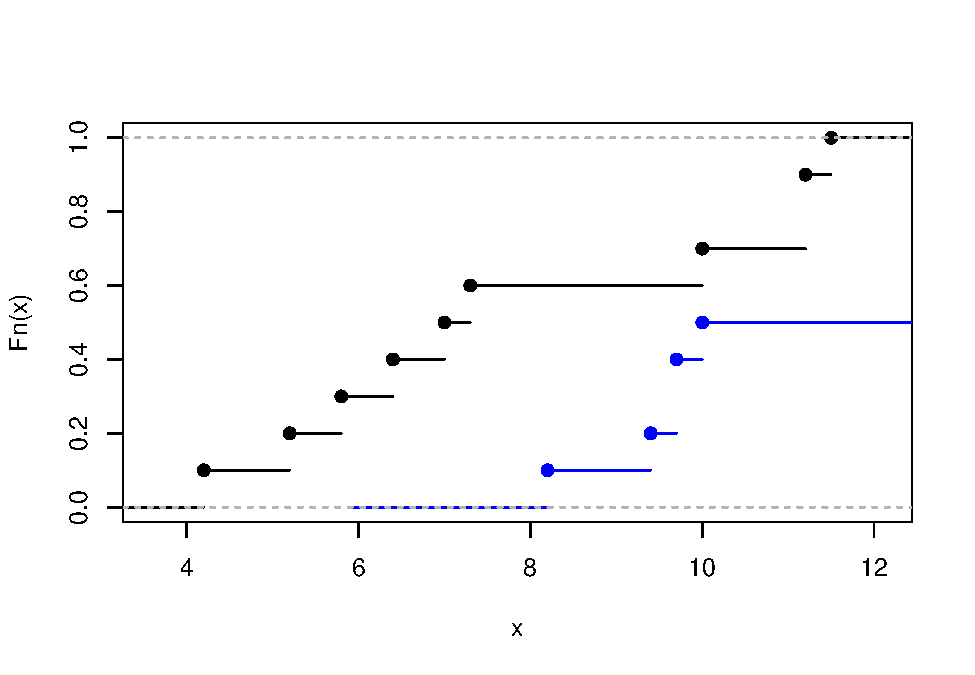
\includegraphics{04-Non-Normal-Responses_files/figure-latex/unnamed-chunk-9-1.pdf}

Finally, compare the the rank-sum test to Student's t-test. The t-test shows an even smaller p-value, but note that the qq-plot shows strong non-normality, which calls into question the appropriateness of the t-test.

\begin{Shaded}
\begin{Highlighting}[]
\NormalTok{my.t.test }\OtherTok{\textless{}{-}} \FunctionTok{t.test}\NormalTok{(ratio.teeth}\SpecialCharTok{\textasciitilde{}}\NormalTok{group, }\AttributeTok{data =}\NormalTok{ teeth)}
\NormalTok{my.t.test}
\end{Highlighting}
\end{Shaded}

\begin{verbatim}
## 
##  Welch Two Sample t-test
## 
## data:  ratio.teeth by group
## t = -3.1697, df = 14.969, p-value = 0.006359
## alternative hypothesis: true difference in means between group 0 and group 1 is not equal to 0
## 95 percent confidence interval:
##  -8.780943 -1.719057
## sample estimates:
## mean in group 0 mean in group 1 
##            7.98           13.23
\end{verbatim}

\begin{Shaded}
\begin{Highlighting}[]
\NormalTok{z }\OtherTok{\textless{}{-}} \FunctionTok{c}\NormalTok{((teeth}\SpecialCharTok{$}\NormalTok{ratio.teeth[teeth}\SpecialCharTok{$}\NormalTok{group}\SpecialCharTok{==}\DecValTok{0}\NormalTok{] }\SpecialCharTok{{-}}\NormalTok{ my.t.test}\SpecialCharTok{$}\NormalTok{estimate[}\DecValTok{1}\NormalTok{]) }\SpecialCharTok{/}\NormalTok{ my.t.test}\SpecialCharTok{$}\NormalTok{stderr, (teeth}\SpecialCharTok{$}\NormalTok{ratio.teeth[teeth}\SpecialCharTok{$}\NormalTok{group}\SpecialCharTok{==}\DecValTok{1}\NormalTok{] }\SpecialCharTok{{-}}\NormalTok{ my.t.test}\SpecialCharTok{$}\NormalTok{estimate[}\DecValTok{2}\NormalTok{]) }\SpecialCharTok{/}\NormalTok{ my.t.test}\SpecialCharTok{$}\NormalTok{stderr)}
\FunctionTok{qqnorm}\NormalTok{(z)}
\FunctionTok{qqline}\NormalTok{(z)}
\end{Highlighting}
\end{Shaded}

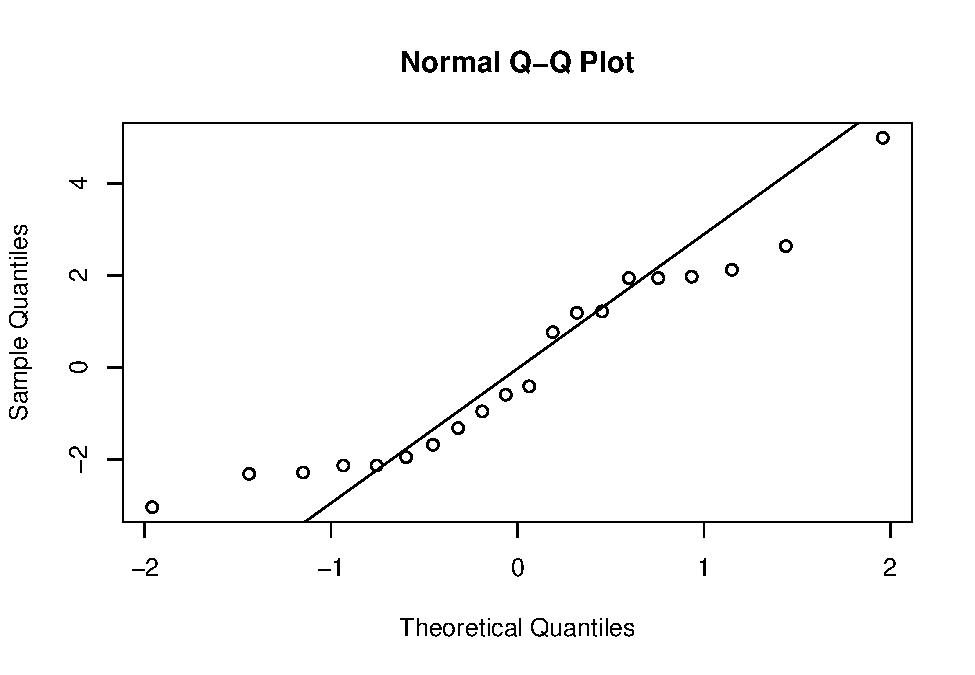
\includegraphics{04-Non-Normal-Responses_files/figure-latex/unnamed-chunk-10-1.pdf}

\hypertarget{signed-rank-test}{%
\section{Signed-rank test}\label{signed-rank-test}}

The signed-rank test or Wilcoxon signed-rank test is the paired analog of the Mann-Whitney test. As an illustrative example we consider a real twins study (not simulated this time) comparing BMIs in pairs of twins.

\begin{Shaded}
\begin{Highlighting}[]
\FunctionTok{library}\NormalTok{(mets)}
\end{Highlighting}
\end{Shaded}

\begin{verbatim}
## Loading required package: timereg
\end{verbatim}

\begin{verbatim}
## Loading required package: survival
\end{verbatim}

\begin{verbatim}
## Loading required package: lava
\end{verbatim}

\begin{verbatim}
## mets version 1.3.0
\end{verbatim}

\begin{Shaded}
\begin{Highlighting}[]
\FunctionTok{data}\NormalTok{(}\StringTok{"twinbmi"}\NormalTok{)}
\FunctionTok{head}\NormalTok{(twinbmi)}
\end{Highlighting}
\end{Shaded}

\begin{verbatim}
##   tvparnr      bmi      age gender zyg id num
## 1       1 26.33289 57.51212   male  DZ  1   1
## 2       1 25.46939 57.51212   male  DZ  1   2
## 3       2 28.65014 56.62696   male  MZ  2   1
## 5       3 28.40909 57.73097   male  DZ  3   1
## 7       4 27.25089 53.68683   male  DZ  4   1
## 8       4 28.07504 53.68683   male  DZ  4   2
\end{verbatim}

\begin{Shaded}
\begin{Highlighting}[]
\NormalTok{twinwide }\OtherTok{\textless{}{-}} \FunctionTok{fast.reshape}\NormalTok{(twinbmi, }\AttributeTok{id=}\StringTok{"tvparnr"}\NormalTok{,}\AttributeTok{varying=}\FunctionTok{c}\NormalTok{(}\StringTok{"bmi"}\NormalTok{))}
\FunctionTok{head}\NormalTok{(twinwide)}
\end{Highlighting}
\end{Shaded}

\begin{verbatim}
##    tvparnr     bmi1      age gender zyg id num     bmi2
## 1        1 26.33289 57.51212   male  DZ  1   1 25.46939
## 3        2 28.65014 56.62696   male  MZ  2   1       NA
## 5        3 28.40909 57.73097   male  DZ  3   1       NA
## 7        4 27.25089 53.68683   male  DZ  4   1 28.07504
## 9        5 27.77778 52.55838   male  DZ  5   1       NA
## 11       6 28.04282 52.52231   male  DZ  6   1 22.30936
\end{verbatim}

\begin{Shaded}
\begin{Highlighting}[]
\NormalTok{twinwide}\SpecialCharTok{$}\NormalTok{bmidiff }\OtherTok{\textless{}{-}}\NormalTok{ (twinwide}\SpecialCharTok{$}\NormalTok{bmi1 }\SpecialCharTok{{-}}\NormalTok{ twinwide}\SpecialCharTok{$}\NormalTok{bmi2)}
\NormalTok{twinwide.cc }\OtherTok{\textless{}{-}} \FunctionTok{complete.cases}\NormalTok{(twinwide)}
\NormalTok{twinwide }\OtherTok{\textless{}{-}}\NormalTok{ twinwide[twinwide.cc,]}
\FunctionTok{head}\NormalTok{(twinwide)}
\end{Highlighting}
\end{Shaded}

\begin{verbatim}
##    tvparnr     bmi1      age gender zyg id num     bmi2  bmidiff
## 1        1 26.33289 57.51212   male  DZ  1   1 25.46939  0.86350
## 7        4 27.25089 53.68683   male  DZ  4   1 28.07504 -0.82415
## 11       6 28.04282 52.52231   male  DZ  6   1 22.30936  5.73346
## 13       7 28.06642 52.62944   male  DZ  7   1 26.51180  1.55462
## 19      10 30.47797 51.24806   male  DZ 10   1 27.66010  2.81787
## 23      12 27.39818 50.02067   male  DZ 12   1 25.97012  1.42806
\end{verbatim}

\begin{Shaded}
\begin{Highlighting}[]
\FunctionTok{dim}\NormalTok{(twinwide)}
\end{Highlighting}
\end{Shaded}

\begin{verbatim}
## [1] 4271    9
\end{verbatim}

The BMI differences may appear normal but actually exhibit \emph{kurtosis}. Since this is an unusual non-normality we will apply a rank transformation.

\begin{Shaded}
\begin{Highlighting}[]
\FunctionTok{hist}\NormalTok{(twinwide}\SpecialCharTok{$}\NormalTok{bmidiff, }\AttributeTok{freq =}\NormalTok{ F)}
\NormalTok{dnorm.tw }\OtherTok{\textless{}{-}} \ControlFlowTok{function}\NormalTok{(x) }\FunctionTok{dnorm}\NormalTok{(x,}\FunctionTok{mean}\NormalTok{(twinwide}\SpecialCharTok{$}\NormalTok{bmidiff), }\FunctionTok{sd}\NormalTok{(twinwide}\SpecialCharTok{$}\NormalTok{bmidiff))}
\FunctionTok{curve}\NormalTok{(dnorm.tw, }\SpecialCharTok{{-}}\DecValTok{20}\NormalTok{,}\DecValTok{20}\NormalTok{, }\AttributeTok{add =} \ConstantTok{TRUE}\NormalTok{)}
\end{Highlighting}
\end{Shaded}

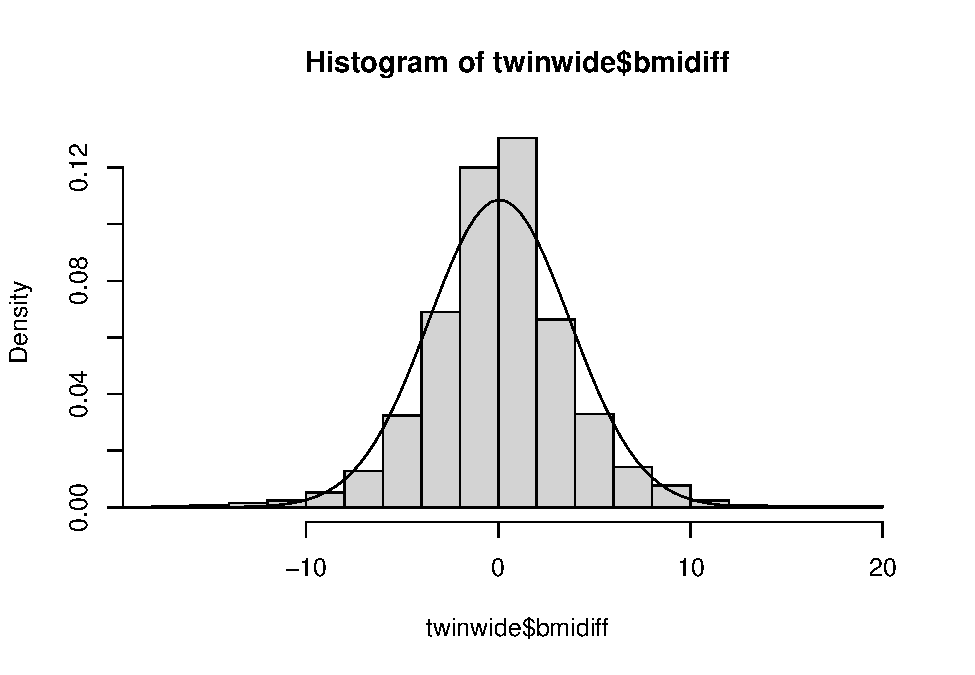
\includegraphics{04-Non-Normal-Responses_files/figure-latex/unnamed-chunk-12-1.pdf}

We can compute the test statistic and p-value by hand as follows: let \(T\) be the sum of the ranks of the absolute BMI differences in the group of positive differences. Then, \(z = (T - \tfrac14n(n+1)) / \sqrt{n(n+1)(2n+1)/24}\) is approximately standard normal.

\begin{Shaded}
\begin{Highlighting}[]
\NormalTok{absdiff }\OtherTok{\textless{}{-}} \FunctionTok{abs}\NormalTok{(twinwide}\SpecialCharTok{$}\NormalTok{bmidiff)}
\NormalTok{signs }\OtherTok{\textless{}{-}} \FunctionTok{ifelse}\NormalTok{(twinwide}\SpecialCharTok{$}\NormalTok{bmidiff}\SpecialCharTok{\textless{}}\DecValTok{0}\NormalTok{,}\SpecialCharTok{{-}}\DecValTok{1}\NormalTok{,}\DecValTok{1}\NormalTok{)}
\NormalTok{n}\OtherTok{\textless{}{-}}\FunctionTok{length}\NormalTok{(signs)}
\NormalTok{sr.nums }\OtherTok{\textless{}{-}} \FunctionTok{cbind}\NormalTok{(absdiff, signs, }\FunctionTok{rank}\NormalTok{(absdiff))}
\NormalTok{sr.nums }\OtherTok{\textless{}{-}}\NormalTok{ sr.nums[}\FunctionTok{order}\NormalTok{(sr.nums[,}\DecValTok{1}\NormalTok{]),]}
\NormalTok{T }\OtherTok{\textless{}{-}} \FunctionTok{sum}\NormalTok{(sr.nums[sr.nums[,}\DecValTok{2}\NormalTok{]}\SpecialCharTok{==}\DecValTok{1}\NormalTok{,}\DecValTok{3}\NormalTok{])}
\NormalTok{z }\OtherTok{\textless{}{-}}\NormalTok{ (T }\SpecialCharTok{{-}}\NormalTok{ n}\SpecialCharTok{*}\NormalTok{(n}\SpecialCharTok{+}\DecValTok{1}\NormalTok{)}\SpecialCharTok{/}\DecValTok{4}\NormalTok{)}\SpecialCharTok{/}\FunctionTok{sqrt}\NormalTok{(n}\SpecialCharTok{*}\NormalTok{(n}\SpecialCharTok{+}\DecValTok{1}\NormalTok{)}\SpecialCharTok{*}\NormalTok{(}\DecValTok{2}\SpecialCharTok{*}\NormalTok{n}\SpecialCharTok{+}\DecValTok{1}\NormalTok{)}\SpecialCharTok{/}\DecValTok{24}\NormalTok{)}
\DecValTok{2}\SpecialCharTok{*}\NormalTok{(}\DecValTok{1}\SpecialCharTok{{-}}\FunctionTok{pnorm}\NormalTok{(}\FunctionTok{abs}\NormalTok{(z)))}
\end{Highlighting}
\end{Shaded}

\begin{verbatim}
## [1] 0.1904966
\end{verbatim}

R has built in functions for the rank-sum and signed-rank tests.

\begin{Shaded}
\begin{Highlighting}[]
\FunctionTok{wilcox.test}\NormalTok{(twinwide}\SpecialCharTok{$}\NormalTok{bmi1, twinwide}\SpecialCharTok{$}\NormalTok{bmi2, }\AttributeTok{paired =} \ConstantTok{TRUE}\NormalTok{)}
\end{Highlighting}
\end{Shaded}

\begin{verbatim}
## 
##  Wilcoxon signed rank test with continuity correction
## 
## data:  twinwide$bmi1 and twinwide$bmi2
## V = 4551983, p-value = 0.2021
## alternative hypothesis: true location shift is not equal to 0
\end{verbatim}

In this case we likely will not come to a different conclusion if we apply Student's t-test.

\begin{Shaded}
\begin{Highlighting}[]
\FunctionTok{t.test}\NormalTok{(twinwide}\SpecialCharTok{$}\NormalTok{bmi1, twinwide}\SpecialCharTok{$}\NormalTok{bmi2, }\AttributeTok{paired =} \ConstantTok{TRUE}\NormalTok{)}
\end{Highlighting}
\end{Shaded}

\begin{verbatim}
## 
##  Paired t-test
## 
## data:  twinwide$bmi1 and twinwide$bmi2
## t = 1.1008, df = 4270, p-value = 0.2711
## alternative hypothesis: true mean difference is not equal to 0
## 95 percent confidence interval:
##  -0.04832046  0.17204938
## sample estimates:
## mean difference 
##      0.06186446
\end{verbatim}

\hypertarget{bootstrap}{%
\section{Bootstrap}\label{bootstrap}}

\hypertarget{intro-to-the-bootstrap}{%
\subsection{Intro to the bootstrap}\label{intro-to-the-bootstrap}}

For hypothesis testing and confidence intervals, there is a ``statistic'' whose sampling distribution is required

For example, to test \(H_0:\mu = \mu_0\) using a normal random sample \(X_1, ..., X_n\) with \(X_i \stackrel{iid}{\sim}N(\mu, \sigma^2)\) the test statistic
\[T = \frac{\bar X - \mu_0}{S/\sqrt{n}}\]
has a \(t\) distribution with \(n-1\) degrees of freedom given the null hypothesis is true.

Only in very simple problems can we determine an ``exact'' test statistic. For example, in the two-sample t-test with unknown, unequal population variances, the T statistic is only approximate.

We often rely on assumptions (like normality) or large sample sizes (CLT) in order to derive approximate (or asymptotic) distributions of statistics.

The bootstrap (in a manner similar to Monte Carlo) tries to approximate the distribution of a test statistic using simulations.

For a distribution with cdf \(F\), we are interested in a parameter \(\theta = \phi(F)\), and functional of \(F\).

Examples:
1. Mean - \(\phi(F) = \int xdF(x)\)
2. Anything else that is a function of moments, like variance
3. Median - \(\phi(F) = \inf\{x: F(x)\geq 0.5\}\)\ldots{}

Given data \(X_1, ..., X_n\) the empirical CDF (think of this as an estimate of \(F\)) is
\[\hat F(x) = \frac{1}{n}\sum_{i=1}^n 1\{X_i \leq x\}.\]

A natural estimate of \(\theta\) is the ``plug-in'' estimator \(\hat\theta = \phi(\hat F)\).

Given the previous setup of CDF and empirical CDF, suppose we want to estimate \(\theta\). If we could somehow simulate from \(F\), then our knowledge of Monte Carlo suggests the following:
1. Simulate many data sets, say \(M\), of size \(n\): \(X_{1,1}, ..., X_{n,1}\), \ldots, \(X_{1,M}, ..., X_{n,M}\).
2. From the \(M\) data sets, compute \(\hat{\theta}_i\) for \(i=1, ..., M\).
3. Then, our many estimates should given us an idea of the mean and the variance of \(\hat{\theta}\).

This actually works when we know the distribution of the test statistic. In the one-sample t-test for a normal mean, the test statistic has a \(t(n-1)\) distribution. So, if we sample from this distribution many times, we will be able to find the rejection region for the hypothesis test by computing Monte Carlo estimates of the \(t(n-1)\) quantiles, but this is rather trivial\ldots{}

Of course, we (usually) cannot simulate from \(F\) because it is unknown (depends on unknown parameters).

Bootstrap idea: Replace simulation from \(F\) with simulation from \(\hat F\)!

Note: it is easy to simulate from \(\hat F\), it's just simulation from a discrete uniform distribution with probabilities \(1/n\) on each data point.

Suppose we are given the following two samples:

\begin{Shaded}
\begin{Highlighting}[]
\FunctionTok{set.seed}\NormalTok{(}\DecValTok{3214354}\NormalTok{)}
\NormalTok{x }\OtherTok{\textless{}{-}} \FunctionTok{rexp}\NormalTok{(}\DecValTok{10}\NormalTok{,}\DecValTok{1}\NormalTok{)}
\NormalTok{y }\OtherTok{\textless{}{-}} \FunctionTok{rexp}\NormalTok{(}\DecValTok{9}\NormalTok{,}\FloatTok{0.8}\NormalTok{)}
\FunctionTok{round}\NormalTok{(x,}\DecValTok{2}\NormalTok{)}
\end{Highlighting}
\end{Shaded}

\begin{verbatim}
##  [1] 0.18 1.30 0.09 1.30 1.73 0.86 1.59 0.60 0.58 0.68
\end{verbatim}

\begin{Shaded}
\begin{Highlighting}[]
\FunctionTok{round}\NormalTok{(y,}\DecValTok{2}\NormalTok{)}
\end{Highlighting}
\end{Shaded}

\begin{verbatim}
## [1] 0.02 0.50 0.41 0.19 0.19 0.69 2.40 1.11 0.11
\end{verbatim}

We could use the t-test, but wait\ldots{}

\begin{Shaded}
\begin{Highlighting}[]
\FunctionTok{par}\NormalTok{(}\AttributeTok{mfrow =} \FunctionTok{c}\NormalTok{(}\DecValTok{1}\NormalTok{,}\DecValTok{2}\NormalTok{))}
\FunctionTok{qqnorm}\NormalTok{(x)}
\FunctionTok{qqline}\NormalTok{(x)}
\FunctionTok{qqnorm}\NormalTok{(y)}
\FunctionTok{qqline}\NormalTok{(y)}
\end{Highlighting}
\end{Shaded}

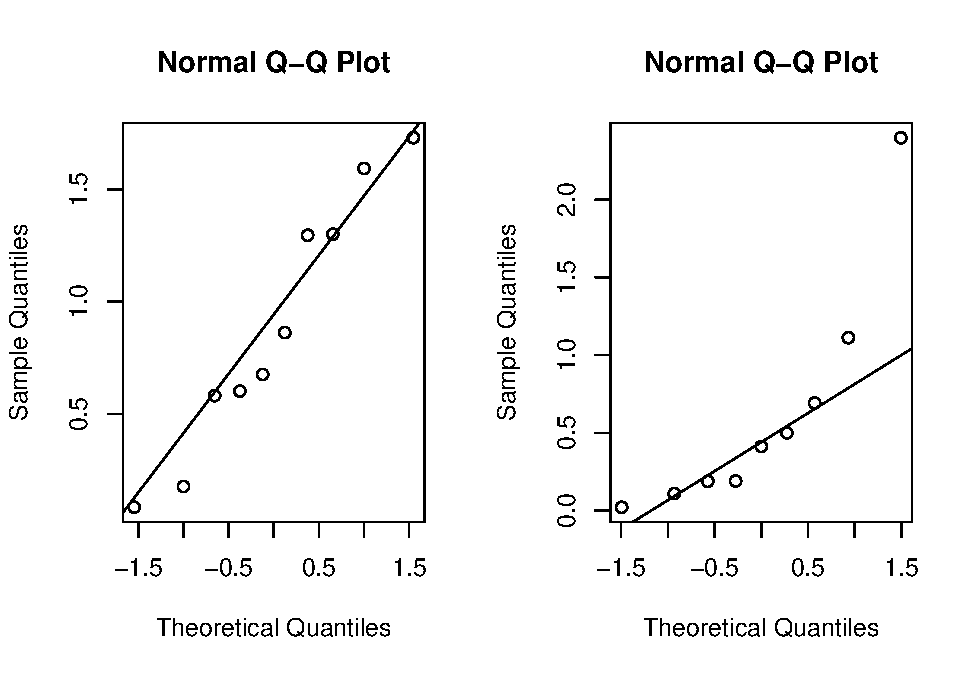
\includegraphics{04-Non-Normal-Responses_files/figure-latex/unnamed-chunk-18-1.pdf}

\begin{Shaded}
\begin{Highlighting}[]
\FunctionTok{shapiro.test}\NormalTok{(x)}
\end{Highlighting}
\end{Shaded}

\begin{verbatim}
## 
##  Shapiro-Wilk normality test
## 
## data:  x
## W = 0.94146, p-value = 0.5694
\end{verbatim}

\begin{Shaded}
\begin{Highlighting}[]
\FunctionTok{shapiro.test}\NormalTok{(y)}
\end{Highlighting}
\end{Shaded}

\begin{verbatim}
## 
##  Shapiro-Wilk normality test
## 
## data:  y
## W = 0.77085, p-value = 0.009449
\end{verbatim}

What ``test statistic'' should I use to test \(H_0:\mu_X = \mu_Y\)? Why not \(\bar X - \bar Y\)?

\begin{Shaded}
\begin{Highlighting}[]
\NormalTok{test.statistic }\OtherTok{\textless{}{-}} \FunctionTok{mean}\NormalTok{(x) }\SpecialCharTok{{-}} \FunctionTok{mean}\NormalTok{(y)}
\NormalTok{boot.test.statistic }\OtherTok{\textless{}{-}} \FunctionTok{rep}\NormalTok{(}\ConstantTok{NA}\NormalTok{, }\DecValTok{10000}\NormalTok{)}
\ControlFlowTok{for}\NormalTok{(i }\ControlFlowTok{in} \DecValTok{1}\SpecialCharTok{:}\DecValTok{10000}\NormalTok{)\{}
\NormalTok{  boot.x }\OtherTok{\textless{}{-}} \FunctionTok{sample}\NormalTok{(x,}\AttributeTok{replace =}\NormalTok{ T)}
\NormalTok{  boot.y }\OtherTok{\textless{}{-}} \FunctionTok{sample}\NormalTok{(y, }\AttributeTok{replace =}\NormalTok{ T)}
\NormalTok{  boot.test.statistic[i] }\OtherTok{\textless{}{-}} \FunctionTok{mean}\NormalTok{(boot.x)}\SpecialCharTok{{-}}\FunctionTok{mean}\NormalTok{(boot.y)}
\NormalTok{\}}
\NormalTok{test.statistic}
\end{Highlighting}
\end{Shaded}

\begin{verbatim}
## [1] 0.2657391
\end{verbatim}

\begin{Shaded}
\begin{Highlighting}[]
\FunctionTok{quantile}\NormalTok{(boot.test.statistic,}\FloatTok{0.025}\NormalTok{)}
\end{Highlighting}
\end{Shaded}

\begin{verbatim}
##      2.5% 
## -0.345881
\end{verbatim}

\begin{Shaded}
\begin{Highlighting}[]
\FunctionTok{quantile}\NormalTok{(boot.test.statistic,}\FloatTok{0.975}\NormalTok{)}
\end{Highlighting}
\end{Shaded}

\begin{verbatim}
##    97.5% 
## 0.792484
\end{verbatim}

\begin{Shaded}
\begin{Highlighting}[]
\NormalTok{m }\OtherTok{\textless{}{-}} \FunctionTok{median}\NormalTok{(boot.test.statistic)}

\NormalTok{approx.p.value }\OtherTok{=} \FunctionTok{ifelse}\NormalTok{(test.statistic }\SpecialCharTok{\textgreater{}}\NormalTok{ m, }\FunctionTok{sum}\NormalTok{((boot.test.statistic}\SpecialCharTok{{-}}\NormalTok{m) }\SpecialCharTok{\textgreater{}}\NormalTok{ (test.statistic }\SpecialCharTok{{-}}\NormalTok{ m))}\SpecialCharTok{/}\DecValTok{10000} \SpecialCharTok{+} \FunctionTok{sum}\NormalTok{((boot.test.statistic}\SpecialCharTok{{-}}\NormalTok{m) }\SpecialCharTok{\textless{}}\NormalTok{ (m}\SpecialCharTok{{-}}\NormalTok{test.statistic))}\SpecialCharTok{/}\DecValTok{10000}\NormalTok{, }\FunctionTok{sum}\NormalTok{((boot.test.statistic}\SpecialCharTok{{-}}\NormalTok{m) }\SpecialCharTok{\textgreater{}}\NormalTok{ (m}\SpecialCharTok{{-}}\NormalTok{test.statistic))}\SpecialCharTok{/}\DecValTok{10000} \SpecialCharTok{+} \FunctionTok{sum}\NormalTok{((boot.test.statistic}\SpecialCharTok{{-}}\NormalTok{m) }\SpecialCharTok{\textless{}}\NormalTok{ (test.statistic}\SpecialCharTok{{-}}\NormalTok{m))}\SpecialCharTok{/}\DecValTok{10000}\NormalTok{ )}
\NormalTok{approx.p.value }
\end{Highlighting}
\end{Shaded}

\begin{verbatim}
## [1] 0.9726
\end{verbatim}

\hypertarget{bootstrap-confidence-intervals}{%
\subsection{Bootstrap Confidence Intervals}\label{bootstrap-confidence-intervals}}

A variety of methods are used to construct confidence intervals using the bootstrap distribution of an estimator. We'll discuss the percentile, basic, and Studentized methods, although several others are available, including the bias-corrected and accelerated (BCa) intervals computed by default in R's boot package.

Suppose the bootstrap samples \(\hat\theta_1, \ldots, \hat\theta_B\) are available. The simplest bootstrap interval estimate is given by the percentile method, which defines the \(100(1-\alpha)\%\) CI to be the \(\alpha/2\) to \((1-\alpha/2)\) sample quantiles of \(\hat\theta_1, \ldots, \hat\theta_B\). There are good arguments against the percentile method, but we won't wade into the details presently. Those arguments tend to favor the basic bootstrap method, which defines the \(100(1-\alpha)\%\) CI to be the interval \((2\overline \theta - \hat\theta_{1-\alpha/2}, \, 2\overline \theta - \hat\theta_{\alpha/2})\), which is twise the sample mean of the bootstrapped estimates minus the \((1-\alpha/2)\) and \(\alpha/2\) sample quantiles of those bootstrapped estimates \(\hat\theta_1, \ldots, \hat\theta_B\).

The last method we'll discuss is the Studentized bootstrap. The idea of the method is to mimic the usual z- or t-test pivotal quantity \(\frac{\hat\theta - \theta}{se(\hat\theta)}\). First, compute \(\hat\theta\) for teh original data. Then, perform the following nested bootstrap, for \(b\) in 1 to \(B\) do:
1.Resample the data with replacement to generate the \(b^{th}\) bootstrap data set
a. for this \(b^{th}\) data set compute the point estimate \(\tilde \theta_b\)
b. Resample the resamples! Generate \(K\) nested bootstrap resamples sample of data. For each of them compute \(\tilde\theta_{b,k}\) for \(k=1, \ldots, K\).
c.~Estimate \(se(\tilde \theta)\) as the standard deviation of \(\tilde\theta_{b,k}\) for \(k=1, \ldots, K\).
d.~Keep the studentized value \(q_b = \frac{\tilde\theta_b - \hat\theta}{se(\tilde\theta_b)}\)
2. Let \(se(\hat\theta)\) be estimated by the sample standard deviation of \(\tilde\theta_1, \ldots, \tilde\theta_B\).
3. Define the Studentized interval as
\[(\hat\theta - q_{1-\alpha/2}se(\hat\theta), \, \hat\theta - q_{\alpha/2}se(\hat\theta))\]
where \(q_\alpha\) is the \(\alpha\) sample quantile of the Studentized \(q\) values.

\begin{Shaded}
\begin{Highlighting}[]
\FunctionTok{set.seed}\NormalTok{(}\DecValTok{3214354}\NormalTok{)}
\NormalTok{x }\OtherTok{\textless{}{-}} \FunctionTok{rexp}\NormalTok{(}\DecValTok{10}\NormalTok{,}\DecValTok{1}\NormalTok{)}
\NormalTok{y }\OtherTok{\textless{}{-}} \FunctionTok{rexp}\NormalTok{(}\DecValTok{9}\NormalTok{,}\FloatTok{0.8}\NormalTok{)}
\FunctionTok{round}\NormalTok{(x,}\DecValTok{2}\NormalTok{)}
\end{Highlighting}
\end{Shaded}

\begin{verbatim}
##  [1] 0.18 1.30 0.09 1.30 1.73 0.86 1.59 0.60 0.58 0.68
\end{verbatim}

\begin{Shaded}
\begin{Highlighting}[]
\FunctionTok{round}\NormalTok{(y,}\DecValTok{2}\NormalTok{)}
\end{Highlighting}
\end{Shaded}

\begin{verbatim}
## [1] 0.02 0.50 0.41 0.19 0.19 0.69 2.40 1.11 0.11
\end{verbatim}

\begin{Shaded}
\begin{Highlighting}[]
\NormalTok{my.boot }\OtherTok{\textless{}{-}} \ControlFlowTok{function}\NormalTok{(x,y, B, K, alpha)\{}
\NormalTok{  hattheta }\OtherTok{\textless{}{-}} \FunctionTok{mean}\NormalTok{(x) }\SpecialCharTok{{-}} \FunctionTok{mean}\NormalTok{(y)}
\NormalTok{  tildetheta }\OtherTok{\textless{}{-}} \FunctionTok{rep}\NormalTok{(}\ConstantTok{NA}\NormalTok{,B)}
\NormalTok{  q }\OtherTok{\textless{}{-}} \FunctionTok{rep}\NormalTok{(}\ConstantTok{NA}\NormalTok{,B)}
  \ControlFlowTok{for}\NormalTok{(b }\ControlFlowTok{in} \DecValTok{1}\SpecialCharTok{:}\NormalTok{B)\{}
\NormalTok{  indices1 }\OtherTok{\textless{}{-}} \FunctionTok{sample}\NormalTok{(}\DecValTok{10}\NormalTok{,}\DecValTok{10}\NormalTok{,}\AttributeTok{replace =} \ConstantTok{TRUE}\NormalTok{)  }
\NormalTok{  indices2 }\OtherTok{\textless{}{-}} \FunctionTok{sample}\NormalTok{(}\DecValTok{9}\NormalTok{,}\DecValTok{9}\NormalTok{,}\AttributeTok{replace =} \ConstantTok{TRUE}\NormalTok{)  }
\NormalTok{  xstar }\OtherTok{\textless{}{-}}\NormalTok{ x[indices1]}
\NormalTok{  ystar }\OtherTok{\textless{}{-}}\NormalTok{ y[indices2]}
\NormalTok{  tildetheta[b] }\OtherTok{\textless{}{-}} \FunctionTok{mean}\NormalTok{(xstar) }\SpecialCharTok{{-}} \FunctionTok{mean}\NormalTok{(ystar)}
\NormalTok{  tilde2 }\OtherTok{\textless{}{-}} \FunctionTok{rep}\NormalTok{(}\ConstantTok{NA}\NormalTok{,K)}
    \ControlFlowTok{for}\NormalTok{(k }\ControlFlowTok{in} \DecValTok{1}\SpecialCharTok{:}\NormalTok{K)\{}
\NormalTok{        indices1 }\OtherTok{\textless{}{-}} \FunctionTok{sample}\NormalTok{(}\DecValTok{10}\NormalTok{,}\DecValTok{10}\NormalTok{,}\AttributeTok{replace =} \ConstantTok{TRUE}\NormalTok{)  }
\NormalTok{        indices2 }\OtherTok{\textless{}{-}} \FunctionTok{sample}\NormalTok{(}\DecValTok{9}\NormalTok{,}\DecValTok{9}\NormalTok{,}\AttributeTok{replace =} \ConstantTok{TRUE}\NormalTok{) }
\NormalTok{        xstar2 }\OtherTok{\textless{}{-}}\NormalTok{ xstar[indices1]}
\NormalTok{        ystar2 }\OtherTok{\textless{}{-}}\NormalTok{ ystar[indices2]}
\NormalTok{        tilde2[k] }\OtherTok{\textless{}{-}} \FunctionTok{mean}\NormalTok{(xstar2)}\SpecialCharTok{{-}}\FunctionTok{mean}\NormalTok{(ystar2)}
\NormalTok{    \}}
\NormalTok{  q[b] }\OtherTok{\textless{}{-}}\NormalTok{ (tildetheta[b] }\SpecialCharTok{{-}}\NormalTok{ hattheta)}\SpecialCharTok{/}\FunctionTok{sd}\NormalTok{(tilde2)}
\NormalTok{  \}}
\NormalTok{  intv }\OtherTok{\textless{}{-}}\NormalTok{ hattheta }\SpecialCharTok{{-}} \FunctionTok{sd}\NormalTok{(tildetheta)}\SpecialCharTok{*}\FunctionTok{quantile}\NormalTok{(q,}\FunctionTok{c}\NormalTok{(}\DecValTok{1}\SpecialCharTok{{-}}\NormalTok{alpha}\SpecialCharTok{/}\DecValTok{2}\NormalTok{,alpha}\SpecialCharTok{/}\DecValTok{2}\NormalTok{))}
  \FunctionTok{return}\NormalTok{(}\FunctionTok{as.numeric}\NormalTok{(intv))}
\NormalTok{\}}
\FunctionTok{my.boot}\NormalTok{(x,y,}\DecValTok{1000}\NormalTok{,}\DecValTok{50}\NormalTok{,}\FloatTok{0.05}\NormalTok{)}
\end{Highlighting}
\end{Shaded}

\begin{verbatim}
## [1] -0.6147748  0.8576096
\end{verbatim}

\hypertarget{bootstrapping-linear-models}{%
\subsection{Bootstrapping linear models}\label{bootstrapping-linear-models}}

When we have only one sample of iid data, bootstrapping is straightforward: simply sample with replacement n times from the original data to obtain a single bootstrap-resampled data set. Repeat many times, recording the estimate corresponding to each resampled set. When there is more ``structure'' present in the data we need to think carefully about how that structure should be treated by the resampling procedure.\\
In linear models, i.e., the Gauss-Markov model, for each response \(Y_i\) there is a corresponding covariate vector \(X_i\). How should these pairs \((Y_i, X_i)\) be treated by the resampling procedure?
One method for bootstrapping a linear model is called row-resampling. Imagine binding the \(n\times 1\) column of responses \(Y\) to the \(n\times p\) matrix of covariates \(X\) and then resampling rows with replacement. We can do this by sampling the integers \(1, \ldots, n\) with replacement, each time taking the corresponding row of \((Y, X)\) as the bootstrap resample. Row resampling treats the pairs \((Y_i, X_i)\) as random, but this is not always reasonable. For example, in a two-sample experiment in which we apply a treatment to 10 of 20 subjects at random and keep the remaining 10 as a control group, row resampling will produce resampled data sets with more than ten in one of the two groups and fewer in the other, which is not how the experiment was performed.
When the \emph{design} is fixed, e.g., we have precisely ten subjects in each group, a different bootstrap method, called residual boostrap, makes more sense. The residual bootstrap starts with the residuals \(e = y - \hat y = y - X_i\hat\beta\). We resample the residuals to obtain \(e^\star = (e_1^\star, \ldots, e_n^\star)^\top\). Next, we compute the bootstrapped responses, \(y_i^\star = X_i\hat\beta + e_i^\star\). Finally, we compute \(\hat\beta^\star\) using \(X\) and \(y^\star\). This way, the design matrix \(X\) remains the same throughout the bootstrap procedure, preserving the structure of the experiment.
Example: Consider the following experiment to evaluate the effect of a bacterial infection on the lifespan of Guinea pigs as measure in days. First, we apply the ro-resampling method. Admittedly, this method makes little sense if we intend for the experiment to have 64 pigs in the control group and 58 in the treatment group.

\begin{Shaded}
\begin{Highlighting}[]
\NormalTok{pigs }\OtherTok{\textless{}{-}} \FunctionTok{read.csv}\NormalTok{(}\StringTok{\textquotesingle{}guinea\_pigs.csv\textquotesingle{}}\NormalTok{)}
\NormalTok{my.lm }\OtherTok{\textless{}{-}} \FunctionTok{lm}\NormalTok{(Time}\SpecialCharTok{\textasciitilde{}}\NormalTok{Treatment, }\AttributeTok{data =}\NormalTok{ pigs)}
\NormalTok{my.lm}
\end{Highlighting}
\end{Shaded}

\begin{verbatim}
## 
## Call:
## lm(formula = Time ~ Treatment, data = pigs)
## 
## Coefficients:
##      (Intercept)  TreatmentControl  
##            242.5             102.7
\end{verbatim}

\begin{Shaded}
\begin{Highlighting}[]
\NormalTok{my.lm}\SpecialCharTok{$}\NormalTok{coefficients}
\end{Highlighting}
\end{Shaded}

\begin{verbatim}
##      (Intercept) TreatmentControl 
##         242.5345         102.6843
\end{verbatim}

\begin{Shaded}
\begin{Highlighting}[]
\NormalTok{n }\OtherTok{\textless{}{-}} \FunctionTok{length}\NormalTok{(pigs}\SpecialCharTok{$}\NormalTok{Pig)}

\NormalTok{r.r.coefs }\OtherTok{\textless{}{-}} \FunctionTok{matrix}\NormalTok{(}\ConstantTok{NA}\NormalTok{,}\DecValTok{1000}\NormalTok{,}\DecValTok{2}\NormalTok{)}
\NormalTok{row.resample.boot }\OtherTok{\textless{}{-}} \ControlFlowTok{function}\NormalTok{(indices)\{}
\NormalTok{  data.star }\OtherTok{\textless{}{-}}\NormalTok{ pigs[indices,]}
\NormalTok{  my.lm }\OtherTok{\textless{}{-}} \FunctionTok{lm}\NormalTok{(Time}\SpecialCharTok{\textasciitilde{}}\NormalTok{Treatment, }\AttributeTok{data =}\NormalTok{ data.star)}
  \FunctionTok{return}\NormalTok{(}\FunctionTok{as.numeric}\NormalTok{(my.lm}\SpecialCharTok{$}\NormalTok{coefficients))}
\NormalTok{\}}
\ControlFlowTok{for}\NormalTok{(i }\ControlFlowTok{in} \DecValTok{1}\SpecialCharTok{:}\DecValTok{1000}\NormalTok{)\{}
\NormalTok{  r.r.coefs[i,] }\OtherTok{\textless{}{-}} \FunctionTok{row.resample.boot}\NormalTok{(}\FunctionTok{sample.int}\NormalTok{(n,n,}\ConstantTok{TRUE}\NormalTok{))}
\NormalTok{\}  }
\NormalTok{r.r.means }\OtherTok{\textless{}{-}} \FunctionTok{colMeans}\NormalTok{(r.r.coefs)}
\NormalTok{percentiles1 }\OtherTok{\textless{}{-}} \FunctionTok{quantile}\NormalTok{(r.r.coefs[,}\DecValTok{1}\NormalTok{], }\FunctionTok{c}\NormalTok{(}\FloatTok{0.05}\NormalTok{,}\FloatTok{0.95}\NormalTok{))}
\NormalTok{percentiles1}
\end{Highlighting}
\end{Shaded}

\begin{verbatim}
##       5%      95% 
## 218.0000 268.3603
\end{verbatim}

\begin{Shaded}
\begin{Highlighting}[]
\NormalTok{percentiles2 }\OtherTok{\textless{}{-}} \FunctionTok{quantile}\NormalTok{(r.r.coefs[,}\DecValTok{2}\NormalTok{], }\FunctionTok{c}\NormalTok{(}\FloatTok{0.05}\NormalTok{,}\FloatTok{0.95}\NormalTok{))}
\NormalTok{percentiles2}
\end{Highlighting}
\end{Shaded}

\begin{verbatim}
##        5%       95% 
##  49.40079 154.59927
\end{verbatim}

\begin{Shaded}
\begin{Highlighting}[]
\FunctionTok{c}\NormalTok{(}\DecValTok{2}\SpecialCharTok{*}\NormalTok{r.r.means[}\DecValTok{1}\NormalTok{] }\SpecialCharTok{{-}}\NormalTok{ percentiles1[}\DecValTok{2}\NormalTok{], }\DecValTok{2}\SpecialCharTok{*}\NormalTok{r.r.means[}\DecValTok{1}\NormalTok{] }\SpecialCharTok{{-}}\NormalTok{ percentiles1[}\DecValTok{1}\NormalTok{])}
\end{Highlighting}
\end{Shaded}

\begin{verbatim}
##      95%       5% 
## 216.4051 266.7653
\end{verbatim}

\begin{Shaded}
\begin{Highlighting}[]
\FunctionTok{c}\NormalTok{(}\DecValTok{2}\SpecialCharTok{*}\NormalTok{r.r.means[}\DecValTok{2}\NormalTok{] }\SpecialCharTok{{-}}\NormalTok{ percentiles2[}\DecValTok{2}\NormalTok{], }\DecValTok{2}\SpecialCharTok{*}\NormalTok{r.r.means[}\DecValTok{2}\NormalTok{] }\SpecialCharTok{{-}}\NormalTok{ percentiles2[}\DecValTok{1}\NormalTok{])}
\end{Highlighting}
\end{Shaded}

\begin{verbatim}
##       95%        5% 
##  50.48009 155.67856
\end{verbatim}

Next, we implement the residual-bootstrap method. Note the two methods give very similar \(90\%\) basic bootstrap CIs for \(\beta_2\) but disagree a bit for \(\beta_1\).

\begin{Shaded}
\begin{Highlighting}[]
\NormalTok{pigs }\OtherTok{\textless{}{-}} 
\FunctionTok{read.csv}\NormalTok{(}\StringTok{\textquotesingle{}guinea\_pigs.csv\textquotesingle{}}\NormalTok{)}
\NormalTok{my.lm }\OtherTok{\textless{}{-}} \FunctionTok{lm}\NormalTok{(Time}\SpecialCharTok{\textasciitilde{}}\NormalTok{Treatment, }\AttributeTok{data =}\NormalTok{ pigs)}
\NormalTok{my.lm}
\end{Highlighting}
\end{Shaded}

\begin{verbatim}
## 
## Call:
## lm(formula = Time ~ Treatment, data = pigs)
## 
## Coefficients:
##      (Intercept)  TreatmentControl  
##            242.5             102.7
\end{verbatim}

\begin{Shaded}
\begin{Highlighting}[]
\NormalTok{my.lm}\SpecialCharTok{$}\NormalTok{coefficients}
\end{Highlighting}
\end{Shaded}

\begin{verbatim}
##      (Intercept) TreatmentControl 
##         242.5345         102.6843
\end{verbatim}

\begin{Shaded}
\begin{Highlighting}[]
\NormalTok{n }\OtherTok{\textless{}{-}} \FunctionTok{length}\NormalTok{(pigs}\SpecialCharTok{$}\NormalTok{Pig)}
\NormalTok{resids }\OtherTok{\textless{}{-}}\NormalTok{ my.lm}\SpecialCharTok{$}\NormalTok{residuals}

\NormalTok{r.r.coefs }\OtherTok{\textless{}{-}} \FunctionTok{matrix}\NormalTok{(}\ConstantTok{NA}\NormalTok{,}\DecValTok{1000}\NormalTok{,}\DecValTok{2}\NormalTok{)}
\NormalTok{resid.boot }\OtherTok{\textless{}{-}} \ControlFlowTok{function}\NormalTok{(indices)\{}
\NormalTok{  resids.star }\OtherTok{\textless{}{-}}\NormalTok{ resids[indices]}
\NormalTok{  y.star }\OtherTok{\textless{}{-}} \FunctionTok{cbind}\NormalTok{(}\FunctionTok{rep}\NormalTok{(}\DecValTok{1}\NormalTok{,n), }\FunctionTok{ifelse}\NormalTok{(pigs}\SpecialCharTok{$}\NormalTok{Treatment}\SpecialCharTok{==}\StringTok{"Control"}\NormalTok{,}\DecValTok{1}\NormalTok{,}\DecValTok{0}\NormalTok{))}\SpecialCharTok{\%*\%}\FunctionTok{matrix}\NormalTok{(}\FunctionTok{as.numeric}\NormalTok{(my.lm}\SpecialCharTok{$}\NormalTok{coefficients),}\DecValTok{2}\NormalTok{,}\DecValTok{1}\NormalTok{) }\SpecialCharTok{+}\NormalTok{ resids.star}
\NormalTok{  data.star }\OtherTok{\textless{}{-}}\NormalTok{ pigs}
\NormalTok{  data.star}\SpecialCharTok{$}\NormalTok{y.star }\OtherTok{\textless{}{-}}\NormalTok{ y.star}
\NormalTok{  my.lm }\OtherTok{\textless{}{-}} \FunctionTok{lm}\NormalTok{(y.star}\SpecialCharTok{\textasciitilde{}}\NormalTok{Treatment, }\AttributeTok{data =}\NormalTok{ data.star)}
  \FunctionTok{return}\NormalTok{(}\FunctionTok{as.numeric}\NormalTok{(my.lm}\SpecialCharTok{$}\NormalTok{coefficients))}
\NormalTok{\}}
\ControlFlowTok{for}\NormalTok{(i }\ControlFlowTok{in} \DecValTok{1}\SpecialCharTok{:}\DecValTok{1000}\NormalTok{)\{}
\NormalTok{  r.r.coefs[i,] }\OtherTok{\textless{}{-}} \FunctionTok{resid.boot}\NormalTok{(}\FunctionTok{sample.int}\NormalTok{(n,n,}\ConstantTok{TRUE}\NormalTok{))}
\NormalTok{\}  }
\NormalTok{r.r.means }\OtherTok{\textless{}{-}} \FunctionTok{colMeans}\NormalTok{(r.r.coefs)}
\NormalTok{percentiles1 }\OtherTok{\textless{}{-}} \FunctionTok{quantile}\NormalTok{(r.r.coefs[,}\DecValTok{1}\NormalTok{], }\FunctionTok{c}\NormalTok{(}\FloatTok{0.05}\NormalTok{,}\FloatTok{0.95}\NormalTok{))}
\NormalTok{percentiles1}
\end{Highlighting}
\end{Shaded}

\begin{verbatim}
##       5%      95% 
## 205.1938 281.0952
\end{verbatim}

\begin{Shaded}
\begin{Highlighting}[]
\NormalTok{percentiles2 }\OtherTok{\textless{}{-}} \FunctionTok{quantile}\NormalTok{(r.r.coefs[,}\DecValTok{2}\NormalTok{], }\FunctionTok{c}\NormalTok{(}\FloatTok{0.05}\NormalTok{,}\FloatTok{0.95}\NormalTok{))}
\NormalTok{percentiles2}
\end{Highlighting}
\end{Shaded}

\begin{verbatim}
##        5%       95% 
##  50.20677 154.69151
\end{verbatim}

\begin{Shaded}
\begin{Highlighting}[]
\FunctionTok{c}\NormalTok{(}\DecValTok{2}\SpecialCharTok{*}\NormalTok{r.r.means[}\DecValTok{1}\NormalTok{] }\SpecialCharTok{{-}}\NormalTok{ percentiles1[}\DecValTok{2}\NormalTok{], }\DecValTok{2}\SpecialCharTok{*}\NormalTok{r.r.means[}\DecValTok{1}\NormalTok{] }\SpecialCharTok{{-}}\NormalTok{ percentiles1[}\DecValTok{1}\NormalTok{])}
\end{Highlighting}
\end{Shaded}

\begin{verbatim}
##      95%       5% 
## 203.5823 279.4838
\end{verbatim}

\begin{Shaded}
\begin{Highlighting}[]
\FunctionTok{c}\NormalTok{(}\DecValTok{2}\SpecialCharTok{*}\NormalTok{r.r.means[}\DecValTok{2}\NormalTok{] }\SpecialCharTok{{-}}\NormalTok{ percentiles2[}\DecValTok{2}\NormalTok{], }\DecValTok{2}\SpecialCharTok{*}\NormalTok{r.r.means[}\DecValTok{2}\NormalTok{] }\SpecialCharTok{{-}}\NormalTok{ percentiles2[}\DecValTok{1}\NormalTok{])}
\end{Highlighting}
\end{Shaded}

\begin{verbatim}
##       95%        5% 
##  52.21648 156.70123
\end{verbatim}

\hypertarget{one-way-anova}{%
\chapter{One Way ANOVA}\label{one-way-anova}}

\hypertarget{the-gauss-markov-model-for-comparing-i-populations}{%
\section{The Gauss-Markov Model for comparing I populations}\label{the-gauss-markov-model-for-comparing-i-populations}}

As we saw in the second chapter, the Gauss-Markov linear model easily extends to comparisons of \(I>2\) populations using either a means or effects parametrization.

In this chapter, we discuss how to compare \(I\) populations efficiently, follow-up tests when not all populations are the same, and how to check model assumptions.

The model we will use throughout is
\[Y = X\beta + \epsilon\]
where \(Y\) is the vector of sampled responses for each of \(I\) groups/populations, \(X\) encodes the group membership structure of the responses, \(\beta\) is an \(I\times 1\) vector that encodes the population means \(\mu_i,\, i=1, \ldots, I\) (not necessarily by the identity function), and \(\epsilon\) is a vector of iid Gaussian random residuals with homogeneous variance \(\sigma^2\).

\hypertarget{example-donuts-effects-model}{%
\subsection{Example: Donuts effects model}\label{example-donuts-effects-model}}

Throughout this chapter we will consider the donuts data: there are 24 observations of oil absorption (in grams above 150 grams) for 4 types of oil (6 replicates per oil, balanced).

\begin{Shaded}
\begin{Highlighting}[]
\NormalTok{donuts }\OtherTok{\textless{}{-}} \FunctionTok{read.csv}\NormalTok{(}\StringTok{\textquotesingle{}donuts.csv\textquotesingle{}}\NormalTok{)}
\FunctionTok{head}\NormalTok{(donuts)}
\end{Highlighting}
\end{Shaded}

\begin{verbatim}
##   Oil  y
## 1   1 14
## 2   1 22
## 3   1 18
## 4   1 27
## 5   1  6
## 6   1 45
\end{verbatim}

\begin{Shaded}
\begin{Highlighting}[]
\NormalTok{donuts}\SpecialCharTok{$}\NormalTok{Oil }\OtherTok{\textless{}{-}} \FunctionTok{factor}\NormalTok{(donuts}\SpecialCharTok{$}\NormalTok{Oil, }\AttributeTok{levels =} \FunctionTok{unique}\NormalTok{(donuts}\SpecialCharTok{$}\NormalTok{Oil))}
\end{Highlighting}
\end{Shaded}

The default R parametrization is an effects model where \(\beta_1\) is the Oil level 1 mean response, and \(\beta_2\) through \(\beta_4\) are differences from baseline, i.e., \(\beta_2 = \mu_{2} - \mu_1\).

\begin{Shaded}
\begin{Highlighting}[]
\NormalTok{my.lm}\OtherTok{\textless{}{-}}\FunctionTok{lm}\NormalTok{(y}\SpecialCharTok{\textasciitilde{}}\NormalTok{Oil, }\AttributeTok{data =}\NormalTok{ donuts)}
\FunctionTok{model.matrix}\NormalTok{(my.lm)}
\end{Highlighting}
\end{Shaded}

\begin{verbatim}
##    (Intercept) Oil2 Oil3 Oil4
## 1            1    0    0    0
## 2            1    0    0    0
## 3            1    0    0    0
## 4            1    0    0    0
## 5            1    0    0    0
## 6            1    0    0    0
## 7            1    1    0    0
## 8            1    1    0    0
## 9            1    1    0    0
## 10           1    1    0    0
## 11           1    1    0    0
## 12           1    1    0    0
## 13           1    0    1    0
## 14           1    0    1    0
## 15           1    0    1    0
## 16           1    0    1    0
## 17           1    0    1    0
## 18           1    0    1    0
## 19           1    0    0    1
## 20           1    0    0    1
## 21           1    0    0    1
## 22           1    0    0    1
## 23           1    0    0    1
## 24           1    0    0    1
## attr(,"assign")
## [1] 0 1 1 1
## attr(,"contrasts")
## attr(,"contrasts")$Oil
## [1] "contr.treatment"
\end{verbatim}

\hypertarget{testing-equality-of-means}{%
\section{Testing equality of means}\label{testing-equality-of-means}}

The ANOVA null hypothesis is equalit of all population means \(H_0:\mu_1 = \mu_2 = \cdots = \mu_I\) versus \(H_a:\text{not all means are equal}\). Given the other assumptions (normality and homogeneous variance) the null hypothesis implies equality of all I populations.

Somewhat counterintuitively, the key to efficiently testing equality of means lies in comparing two different estimators of the common variance \(\sigma^2\). Consider the pooled variance estimator:
\[MSE = \frac{1}{N-I}\sum_{i=1}^I\sum_{j=1}^{n_i}(Y_{ij} - \bar Y_{i\cdot})^2\]
where the subscript \(i\) denotes the group membership and the subscript \(j\) denotes the individual within group \(i\); \(N = \sum_{i=1}^I n_i\) where \(n_i\) is the \(i^{th}\) group's sample size. Clearly, the mean squared error (MSE, also called mean within group variability or MSW) is a pooled variance estimator, equal to the pooled sample variance \(S_p^2\) when \(I=2\). It is straightforward to show \(MSE\) is unbiased for \(\sigma^2\), given that the sample variance in each group is unbiased for the variance. Furthermore, since \(\sum_{j=1}^{n_i}(Y_{ij} - \bar Y_{i\cdot})^2\) divided by \(\sigma^2\) follows a Chi-squared distribution with \(n_i - 1\) degrees of freedom, and since sums of independent Chi-squared r.v.'s are Chi-squared with df equal to the sum of degrees of freedom of the summand r.v.'s it follows that
\[\frac{MSE}{\sigma^2}\sim \chi^2(N-I).\]

Similarly, suppose the null hypothesis above is true and all the means are the same. Then, \(\bar Y_{i\cdot}\stackrel{ind}{\sim}N(\mu, \sigma^2/n_i)\), and another unbiased estimator of \(\sigma^2\) is given by
\[MSTr = \sum_{i=1}^I n_i(\bar Y_{i\cdot}-\bar Y_{\cdot\cdot})^2,\]
which is the mean square of treatments (or mean between group variation MSB). However, this is clearly only unbiased under \(H_0\), because under \(H_a\) the observed residuals inside the sum of squares are not centered. Indeed, under the alternative hypothesis, it is not hard (but is tedious) to show that
\[E(MSTr) = \sigma^2 + \frac{1}{I-1}\sum_{i=1}^I n_i(\mu_i - \bar\mu)^2\]
where \(\bar\mu = N^{-1}\sum_{i=1}^In_i\mu_i\). The bias term is positive, which suggests a one-sided test of \(H_0\) determined by the ratio \(MSTr/MSE\). All we need is the sampling distribution of that statistic. For essentially the same reason as above, it follows that \(MSTr\) follows a Chi-squared distribution with df \(I-1\) under \(H_0\). It's less obvious that MSTr and MSE are independent, but they are. Very briefly, the reason is that both of these statistics are \emph{quadratic forms} that may be written \(MSE = Y^\top AY\) and \(MSTr = Y^\top BY\) for some matrices \(A\) and \(B\). Multivariate normal distribution theory says that quadratic forms are independent if \(A\) and \(B\) are orthogonal matrices. Some careful work will show MSE and MSTr satisfy this property. Then, their ratio is a ratio of independent Chi-squared r.v.'s, which is an F r.v.:
\[F=\frac{MSTr}{MSE}\stackrel{H_0}{\sim}F(I-1, N-I).\]
Recall that only large values of this ratio suggest the null hypothesis is incorrect, and, therefore, we reject \(H_0\) at level \(\alpha\) if \(F>F_{1-\alpha, I-1, N-I}\). This is called the analysis of variance (ANOVA) F test.

\textless\textless\textless\textless\textless\textless\textless{} HEAD
\#\#\# Example: Donuts

Below we evaluate the F test for equality of mean oil absorption across all four types of oil. ``By hand'' we find a p-value of 0.0069, which suggests we should reject the null hypothesis of equal means and conclude different oils have different average absorption. Alternatively, the built-in \({\tt aov}\) function will compute the F statistic and p-value, and display both using the \({\tt summary}\) utility function.

\begin{Shaded}
\begin{Highlighting}[]
\FunctionTok{library}\NormalTok{(tidyverse)}
\end{Highlighting}
\end{Shaded}

\begin{verbatim}
## -- Attaching packages --------------------------------------- tidyverse 1.3.2 --
## v ggplot2 3.3.6      v purrr   0.3.4 
## v tibble  3.1.8      v dplyr   1.0.10
## v tidyr   1.2.1      v stringr 1.4.1 
## v readr   2.1.2      v forcats 0.5.2 
## -- Conflicts ------------------------------------------ tidyverse_conflicts() --
## x dplyr::filter() masks stats::filter()
## x dplyr::lag()    masks stats::lag()
\end{verbatim}

\begin{Shaded}
\begin{Highlighting}[]
\NormalTok{by\_oil }\OtherTok{\textless{}{-}} \FunctionTok{group\_by}\NormalTok{(donuts, Oil)}
\NormalTok{means }\OtherTok{\textless{}{-}} \FunctionTok{summarise}\NormalTok{(by\_oil, }\AttributeTok{means =} \FunctionTok{mean}\NormalTok{(y))}
\NormalTok{SSE }\OtherTok{\textless{}{-}} \FunctionTok{sum}\NormalTok{((donuts}\SpecialCharTok{$}\NormalTok{y[donuts}\SpecialCharTok{$}\NormalTok{Oil}\SpecialCharTok{==}\DecValTok{1}\NormalTok{] }\SpecialCharTok{{-}}\NormalTok{ means}\SpecialCharTok{$}\NormalTok{means[}\DecValTok{1}\NormalTok{])}\SpecialCharTok{\^{}}\DecValTok{2}\NormalTok{) }\SpecialCharTok{+} \FunctionTok{sum}\NormalTok{((donuts}\SpecialCharTok{$}\NormalTok{y[donuts}\SpecialCharTok{$}\NormalTok{Oil}\SpecialCharTok{==}\DecValTok{2}\NormalTok{] }\SpecialCharTok{{-}}\NormalTok{ means}\SpecialCharTok{$}\NormalTok{means[}\DecValTok{2}\NormalTok{])}\SpecialCharTok{\^{}}\DecValTok{2}\NormalTok{)}\SpecialCharTok{+}\FunctionTok{sum}\NormalTok{((donuts}\SpecialCharTok{$}\NormalTok{y[donuts}\SpecialCharTok{$}\NormalTok{Oil}\SpecialCharTok{==}\DecValTok{3}\NormalTok{] }\SpecialCharTok{{-}}\NormalTok{ means}\SpecialCharTok{$}\NormalTok{means[}\DecValTok{3}\NormalTok{])}\SpecialCharTok{\^{}}\DecValTok{2}\NormalTok{)}\SpecialCharTok{+}\FunctionTok{sum}\NormalTok{((donuts}\SpecialCharTok{$}\NormalTok{y[donuts}\SpecialCharTok{$}\NormalTok{Oil}\SpecialCharTok{==}\DecValTok{4}\NormalTok{] }\SpecialCharTok{{-}}\NormalTok{ means}\SpecialCharTok{$}\NormalTok{means[}\DecValTok{4}\NormalTok{])}\SpecialCharTok{\^{}}\DecValTok{2}\NormalTok{)}
\NormalTok{SSTr }\OtherTok{\textless{}{-}} \DecValTok{6}\SpecialCharTok{*}\NormalTok{((means}\SpecialCharTok{$}\NormalTok{means[}\DecValTok{1}\NormalTok{] }\SpecialCharTok{{-}} \FunctionTok{mean}\NormalTok{(donuts}\SpecialCharTok{$}\NormalTok{y))}\SpecialCharTok{\^{}}\DecValTok{2}\NormalTok{)}\SpecialCharTok{+}\DecValTok{6}\SpecialCharTok{*}\NormalTok{((means}\SpecialCharTok{$}\NormalTok{means[}\DecValTok{2}\NormalTok{] }\SpecialCharTok{{-}} \FunctionTok{mean}\NormalTok{(donuts}\SpecialCharTok{$}\NormalTok{y))}\SpecialCharTok{\^{}}\DecValTok{2}\NormalTok{)}\SpecialCharTok{+}\DecValTok{6}\SpecialCharTok{*}\NormalTok{((means}\SpecialCharTok{$}\NormalTok{means[}\DecValTok{3}\NormalTok{] }\SpecialCharTok{{-}} \FunctionTok{mean}\NormalTok{(donuts}\SpecialCharTok{$}\NormalTok{y))}\SpecialCharTok{\^{}}\DecValTok{2}\NormalTok{)}\SpecialCharTok{+}\DecValTok{6}\SpecialCharTok{*}\NormalTok{((means}\SpecialCharTok{$}\NormalTok{means[}\DecValTok{4}\NormalTok{] }\SpecialCharTok{{-}} \FunctionTok{mean}\NormalTok{(donuts}\SpecialCharTok{$}\NormalTok{y))}\SpecialCharTok{\^{}}\DecValTok{2}\NormalTok{)}
\NormalTok{F }\OtherTok{\textless{}{-}}\NormalTok{ (SSTr}\SpecialCharTok{/}\DecValTok{3}\NormalTok{)}\SpecialCharTok{/}\NormalTok{(SSE}\SpecialCharTok{/}\NormalTok{(}\DecValTok{6}\SpecialCharTok{*}\DecValTok{4{-}4}\NormalTok{))}
\NormalTok{SSE}
\end{Highlighting}
\end{Shaded}

\begin{verbatim}
## [1] 2018
\end{verbatim}

\begin{Shaded}
\begin{Highlighting}[]
\NormalTok{SSTr}
\end{Highlighting}
\end{Shaded}

\begin{verbatim}
## [1] 1636.5
\end{verbatim}

\begin{Shaded}
\begin{Highlighting}[]
\NormalTok{F}
\end{Highlighting}
\end{Shaded}

\begin{verbatim}
## [1] 5.406343
\end{verbatim}

\begin{Shaded}
\begin{Highlighting}[]
\NormalTok{p.value }\OtherTok{\textless{}{-}} \DecValTok{1}\SpecialCharTok{{-}}\FunctionTok{pf}\NormalTok{(F, }\DecValTok{4{-}1}\NormalTok{, }\DecValTok{6}\SpecialCharTok{*}\DecValTok{4} \SpecialCharTok{{-}} \DecValTok{4}\NormalTok{)}
\NormalTok{p.value}
\end{Highlighting}
\end{Shaded}

\begin{verbatim}
## [1] 0.006875948
\end{verbatim}

\begin{Shaded}
\begin{Highlighting}[]
\NormalTok{my.aov }\OtherTok{\textless{}{-}} \FunctionTok{aov}\NormalTok{(y}\SpecialCharTok{\textasciitilde{}}\NormalTok{Oil, }\AttributeTok{data=}\NormalTok{donuts)}
\FunctionTok{summary}\NormalTok{(my.aov)}
\end{Highlighting}
\end{Shaded}

\begin{verbatim}
##             Df Sum Sq Mean Sq F value  Pr(>F)   
## Oil          3   1636   545.5   5.406 0.00688 **
## Residuals   20   2018   100.9                   
## ---
## Signif. codes:  0 '***' 0.001 '**' 0.01 '*' 0.05 '.' 0.1 ' ' 1
\end{verbatim}

\hypertarget{follow-up-testing}{%
\section{Follow-up testing}\label{follow-up-testing}}

When we reject the null hypothesis of equal means we usually want to know the answer to the follow-up question ``which means are actually different''? It may be that one population mean is different from the others, which are all the same; or, it could be that every mean is different. If this question affects the actions the experimenters would take or recommend, then a follow-up test to evaluate these possibilities is valuable.

The most straightforward way to conduct such a follow-up test would be to compare all the means pairwise and use a Bonferroni correction to account for the multiple tests. This is not the most powerful testing method. A much better method was developed by Tukey for use specifically with one-way ANOVA.

Tukey's procedure is based on a sampling distribution he derived called \textbf{Tukey's Studentized Range distribution}. If \(Z_i\) for \(i=1,\ldots, n\) are iid standard normal random variables and \(W\) is a Chi-Squared random variable with \(\nu\) degrees of freedom independent from the \(Z_i\)'s then the random variable
\[T = \frac{\max_{i\ne j}|Z_i - Z_j|}{\sqrt{W/\nu}}\]
follows Tukey's distribution with two degrees of freedom parameters, \(n\) and \(\nu\).

First, consider a balanced experiment, meaning we collect a random sample \(Y_{i1, \ldots, Y_{i,n}}\) of size \(n\) from every population, \(i=1, \ldots, I\). We know that \(n(I-1)MSE/\sigma^2\) has a Chi-squared distribution with \(nI-I = n(I-1)\) degrees of freedom, and is independent from \(\overline Y_{i\cdot}\) for \(i=1, \ldots, I\) (essentially by Student's Theorem). The variance of \(\overline Y_{i\cdot} - \overline Y_{j\cdot}\) is \(\sigma^2(1/n + 1/n)\). Therefore,
\[T = \frac{\max_{i\ne j}\left|\frac{\overline Y_{i\cdot}}{\sigma\sqrt{1/n}} - \frac{\overline Y_{j\cdot}}{{\sigma\sqrt{1/n}}}\right|}{\sqrt{n(I-1)MSE/\sigma^2}} = \frac{\max_{i\ne j}\left|\overline Y_{i\cdot} - \overline Y_{j\cdot}\right|}{\sqrt{MSE/n}}\]
follows Tukey's distribution with degrees of freedom \(I\) and \(n(I-1)\).

Another way Tukey's test statistic is often written is
\[T = \frac{\max_{i\ne j}\left|\overline Y_{i\cdot} - \overline Y_{j\cdot}\right|}{2^{-1/2}\sqrt{MSE(2/n)}},\]
which may be easier to remember because the standard error of \(\overline Y_{i\cdot} - \overline Y_{j\cdot}\) is \(2\sigma^2/n\).

Tukey's procedure says to do the following:
1. Evaluate the test statistics \(T_{i,j}\) for all \({n\choose 2}\) pairs where
\[T_{i,j} = \frac{\left|\overline Y_{i\cdot} - \overline Y_{j\cdot}\right|}{2^{-1/2}\sqrt{MSE(2/n)}}.\]
2. Conclude \(\mu_i\) and \(\mu_j\) are significantly different at level \(\alpha\) if \(T_{i,j} > q_{1-\alpha, n, n(I-1)}\) where \(q_{\alpha,u,v}\) is the \(\alpha^{th}\) quantile of Tukey's distribution with \(u\) and \(v\) degrees of freedom.
-OR-
1. Evaluate the \({n\choose 2}\) confidence intervals
\[(\overline Y_{i\cdot} - \overline Y_{j\cdot}\pm 2^{-1/2}q_{1-\alpha, n, n(I-1)}\sqrt{MSE(2/n)}).\]
2. For every interval \textbf{not} including zero, conclude the corresponding means are significantly different.

Both procedures, the testing procedure and the confidence interval procedure, maintain Type 1 error at level \(\alpha\) collectively over all \({n \choose 2}\) pairwise comparisons.

When the experiment is \textbf{unbalanced}---meaning that the sample sizes of the samples taken from each of the \(I\) populations are not all equal, Tukey's procedure is approximate. In that case, Tukey's statistic
\[T_{i,j} = \frac{\left|\overline Y_{i\cdot} - \overline Y_{j\cdot}\right|}{2^{-1/2}\sqrt{MSE\left(\frac{1}{n_i}+\frac{1}{n_j}\right)}}\]
only approximately follows Tukey's studentized range distribution with degrees of freedom \(I\) and \(N-I\) where \(N = \sum_{i=1}^I n_i\). Tukey's procedure for unbalanced experiments is exactly the same, but the family-wise (over all comparisons) Type 1 error is only approximately controlled at level \(\alpha\).

\hypertarget{donuts-example}{%
\subsection{Donuts example}\label{donuts-example}}

Tukey's simultaneous pairwise comparisons may be performed in R using either the built-in TukeyHSD function or the emmeans and contrast functions in the emmeans package. The former performs the confidence interval procedure whereas the latter performs the test statistic procedure, but either way you will obtain the same results.

At level \(5\%\) only oils 2 and 4 had significantly different mean absorption. Note that the 4-2 CI does not contain zero, or, alternatively, that Oil2 - Oil4 p-value if 0.0039, the only one smaller than 0.05.

\begin{Shaded}
\begin{Highlighting}[]
\FunctionTok{TukeyHSD}\NormalTok{(my.aov)}
\end{Highlighting}
\end{Shaded}

\begin{verbatim}
##   Tukey multiple comparisons of means
##     95% family-wise confidence level
## 
## Fit: aov(formula = y ~ Oil, data = donuts)
## 
## $Oil
##     diff        lwr       upr     p adj
## 2-1   13  -3.232221 29.232221 0.1461929
## 3-1    4 -12.232221 20.232221 0.8998057
## 4-1  -10 -26.232221  6.232221 0.3378150
## 3-2   -9 -25.232221  7.232221 0.4270717
## 4-2  -23 -39.232221 -6.767779 0.0039064
## 4-3  -14 -30.232221  2.232221 0.1065573
\end{verbatim}

\begin{Shaded}
\begin{Highlighting}[]
\FunctionTok{library}\NormalTok{(emmeans) }
\NormalTok{fit.emm }\OtherTok{\textless{}{-}} \FunctionTok{emmeans}\NormalTok{(my.aov, }\StringTok{"Oil"}\NormalTok{)}
\FunctionTok{summary}\NormalTok{(}\FunctionTok{contrast}\NormalTok{(fit.emm, }\AttributeTok{method =} \StringTok{"pairwise"}\NormalTok{))}
\end{Highlighting}
\end{Shaded}

\begin{verbatim}
##  contrast    estimate  SE df t.ratio p.value
##  Oil1 - Oil2      -13 5.8 20  -2.242  0.1462
##  Oil1 - Oil3       -4 5.8 20  -0.690  0.8998
##  Oil1 - Oil4       10 5.8 20   1.724  0.3378
##  Oil2 - Oil3        9 5.8 20   1.552  0.4271
##  Oil2 - Oil4       23 5.8 20   3.966  0.0039
##  Oil3 - Oil4       14 5.8 20   2.414  0.1066
## 
## P value adjustment: tukey method for comparing a family of 4 estimates
\end{verbatim}

\hypertarget{inference-for-particular-contrasts}{%
\section{Inference for particular contrasts}\label{inference-for-particular-contrasts}}

Besides pairwise comparisons, experimenters may be interested in comparing particular combinations of treatment means. For example, they may want to answer the question: ``Is Oil 4 significantly different than Oils 1-3 combined?'' in the contest of the donuts experiment. This is not a pairwise comparison; rather, it's a linear combination (or contrast) defined by \(\mu_4 - \tfrac13(\mu_1+\mu_2+\mu_3)\). It is important that we decide which contrasts to test \emph{apriori}---that is, before we do the experiment. We do not want to bias our test procedures by using the data to suggest which contrasts might be significant and then testing those in particular. That practice leads to inflated Type 1 error. Likewise, when testing multiple contrasts, it is a good idea to make a Type 1 correction for multiple tests if a decision or action hinges on the outcome of the tests in total. For this correction we need something new, because Tukey's procedure only works for pairwise comparisons, and contrasts are more general objects.

In general, a contrast may be written \(\gamma = \sum_{i=1}^I c_i\mu_i = c^\top \mu\) where \(0=\sum_{i=1}^I c_i\). The estimated contrast is \(\hat\gamma = \sum_{i=1}^n c_i\overline Y_{i\cdot}\) and it has standard error \(\sqrt{\sigma^2\sum_{i=1}^n (c_i^2/n_i)}\). It follows that tests and CIs for \(\gamma\) are based on the follow Student's t r.v.:
\[\frac{\hat\gamma - \gamma}{\sqrt{\sigma^2\sum_{i=1}^n (c_i^2/n_i)}}\sim t_{N-I}.\]

Scheff\textquotesingle e developed a correction for simultaneous inference on several (even all possible) contrasts. This method is prefereable to Bonferroni for more than a few contrasts, but will be overly conservative for just two or three contrasts. Scheff\textquotesingle e says to use cutoffs of the form \(\sqrt{(I-1)F_{1-\alpha, I-1, N-I}}\) rather than Student's t quantiles \(t_{1-\alpha/2, N-I}\) for tests of contrasts and for margin of error expressions for CIs of contrasts. In particular, Scheff\textquotesingle e's CIs for contrasts \(\gamma_\ell\), \(\ell=1,\ldots\) are
\[\left(\hat\gamma_\ell \pm \sqrt{(I-1)F_{1-\alpha, I-1, N-I}}\sqrt{MSE\sum_{i=1}^n (c_i^2/n_i)}\right).\]
This collection of CIs has coverage \(100(1-\alpha)\%\) for any vector of contrasts \(\gamma = (\gamma_1, \gamma_2, \ldots )\).

\hypertarget{donuts-example-1}{%
\subsection{Donuts Example}\label{donuts-example-1}}

Below we compute CIs for the contrast comparing Oil 4 to the average of Oils 1-3 and p-values for the test of \(\gamma = 0\) using both the single contrast methods based on the Student's t sampling distribution and Scheffe's correction for inference on all simultaneous contrasts. Using the emmeans package we can do these computations with built-in functions rather than ``by hand''. Note that the p-value using Scheff\textquotesingle e's method is about ten times higher than the single contrast method, which demonstrates the correction for inference on all contrasts is substantial.

\begin{Shaded}
\begin{Highlighting}[]
\NormalTok{MSE }\OtherTok{\textless{}{-}}\NormalTok{ SSE}\SpecialCharTok{/}\NormalTok{(}\DecValTok{6}\SpecialCharTok{*}\DecValTok{4{-}4}\NormalTok{)}
\NormalTok{c1 }\OtherTok{\textless{}{-}} \FunctionTok{c}\NormalTok{(}\SpecialCharTok{{-}}\DecValTok{1}\SpecialCharTok{/}\DecValTok{3}\NormalTok{, }\SpecialCharTok{{-}}\DecValTok{1}\SpecialCharTok{/}\DecValTok{3}\NormalTok{, }\SpecialCharTok{{-}}\DecValTok{1}\SpecialCharTok{/}\DecValTok{3}\NormalTok{, }\DecValTok{1}\NormalTok{)}
\NormalTok{gamma.hat }\OtherTok{\textless{}{-}} \FunctionTok{sum}\NormalTok{(c1}\SpecialCharTok{*}\NormalTok{means}\SpecialCharTok{$}\NormalTok{means)}
\NormalTok{se }\OtherTok{\textless{}{-}} \FunctionTok{sqrt}\NormalTok{(MSE}\SpecialCharTok{*}\FunctionTok{sum}\NormalTok{((c1}\SpecialCharTok{\^{}}\DecValTok{2}\NormalTok{)}\SpecialCharTok{*}\NormalTok{(}\DecValTok{1}\SpecialCharTok{/}\DecValTok{6}\NormalTok{)))}
\FunctionTok{c}\NormalTok{(gamma.hat }\SpecialCharTok{{-}} \FunctionTok{qt}\NormalTok{(}\FloatTok{0.975}\NormalTok{,}\DecValTok{4}\SpecialCharTok{*}\DecValTok{6{-}4}\NormalTok{)}\SpecialCharTok{*}\NormalTok{se,gamma.hat }\SpecialCharTok{+} \FunctionTok{qt}\NormalTok{(}\FloatTok{0.975}\NormalTok{,}\DecValTok{4}\SpecialCharTok{*}\DecValTok{6{-}4}\NormalTok{)}\SpecialCharTok{*}\NormalTok{se)}
\end{Highlighting}
\end{Shaded}

\begin{verbatim}
## [1] -25.54414  -5.78919
\end{verbatim}

\begin{Shaded}
\begin{Highlighting}[]
\DecValTok{2}\SpecialCharTok{*}\FunctionTok{pt}\NormalTok{(gamma.hat}\SpecialCharTok{/}\NormalTok{se, }\DecValTok{4}\SpecialCharTok{*}\DecValTok{6{-}4}\NormalTok{)}
\end{Highlighting}
\end{Shaded}

\begin{verbatim}
## [1] 0.003506899
\end{verbatim}

\begin{Shaded}
\begin{Highlighting}[]
\FunctionTok{c}\NormalTok{(gamma.hat }\SpecialCharTok{{-}} \FunctionTok{sqrt}\NormalTok{((}\DecValTok{4{-}1}\NormalTok{)}\SpecialCharTok{*}\FunctionTok{qf}\NormalTok{(}\FloatTok{0.95}\NormalTok{,}\DecValTok{4{-}1}\NormalTok{,}\DecValTok{4}\SpecialCharTok{*}\DecValTok{6{-}4}\NormalTok{))}\SpecialCharTok{*}\NormalTok{se,gamma.hat }\SpecialCharTok{+} \FunctionTok{sqrt}\NormalTok{((}\DecValTok{4{-}1}\NormalTok{)}\SpecialCharTok{*}\FunctionTok{qf}\NormalTok{(}\FloatTok{0.95}\NormalTok{,}\DecValTok{4{-}1}\NormalTok{,}\DecValTok{4}\SpecialCharTok{*}\DecValTok{6{-}4}\NormalTok{))}\SpecialCharTok{*}\NormalTok{se)}
\end{Highlighting}
\end{Shaded}

\begin{verbatim}
## [1] -30.103372  -1.229962
\end{verbatim}

\begin{Shaded}
\begin{Highlighting}[]
\DecValTok{1}\SpecialCharTok{{-}}\FunctionTok{pf}\NormalTok{((gamma.hat}\SpecialCharTok{/}\NormalTok{(se}\SpecialCharTok{*}\FunctionTok{sqrt}\NormalTok{(}\DecValTok{4{-}1}\NormalTok{)))}\SpecialCharTok{\^{}}\DecValTok{2}\NormalTok{, }\DecValTok{4{-}1}\NormalTok{,}\DecValTok{4}\SpecialCharTok{*}\DecValTok{6{-}4}\NormalTok{)}
\end{Highlighting}
\end{Shaded}

\begin{verbatim}
## [1] 0.03014771
\end{verbatim}

\begin{Shaded}
\begin{Highlighting}[]
\FunctionTok{library}\NormalTok{(emmeans) }\CommentTok{\# may need to install.packages(\textquotesingle{}emmeans\textquotesingle{})}
\NormalTok{fit.emm }\OtherTok{\textless{}{-}} \FunctionTok{emmeans}\NormalTok{(my.aov, }\StringTok{"Oil"}\NormalTok{)}
\CommentTok{\# unadjusted, just testing one contrast}
\FunctionTok{summary}\NormalTok{(}\FunctionTok{contrast}\NormalTok{(fit.emm, }\AttributeTok{method =} \FunctionTok{list}\NormalTok{(}\FunctionTok{c}\NormalTok{(}\SpecialCharTok{{-}}\DecValTok{1}\SpecialCharTok{/}\DecValTok{3}\NormalTok{, }\SpecialCharTok{{-}}\DecValTok{1}\SpecialCharTok{/}\DecValTok{3}\NormalTok{, }\SpecialCharTok{{-}}\DecValTok{1}\SpecialCharTok{/}\DecValTok{3}\NormalTok{, }\DecValTok{1}\NormalTok{))))}
\end{Highlighting}
\end{Shaded}

\begin{verbatim}
##  contrast                                                       estimate   SE
##  c(-0.333333333333333, -0.333333333333333, -0.333333333333333,     -15.7 4.74
##  df t.ratio p.value
##  20  -3.309  0.0035
\end{verbatim}

\begin{Shaded}
\begin{Highlighting}[]
\CommentTok{\# Scheffe adjustment so that we could test all linear contrasts}
\FunctionTok{summary}\NormalTok{(}\FunctionTok{contrast}\NormalTok{(fit.emm, }\AttributeTok{method =} \FunctionTok{list}\NormalTok{(}\FunctionTok{c}\NormalTok{(}\SpecialCharTok{{-}}\DecValTok{1}\SpecialCharTok{/}\DecValTok{3}\NormalTok{, }\SpecialCharTok{{-}}\DecValTok{1}\SpecialCharTok{/}\DecValTok{3}\NormalTok{, }\SpecialCharTok{{-}}\DecValTok{1}\SpecialCharTok{/}\DecValTok{3}\NormalTok{, }\DecValTok{1}\NormalTok{)), }
                 \AttributeTok{adjust =} \StringTok{"scheffe"}\NormalTok{), }\AttributeTok{scheffe.rank =} \DecValTok{3}\NormalTok{)}
\end{Highlighting}
\end{Shaded}

\begin{verbatim}
##  contrast                                                       estimate   SE
##  c(-0.333333333333333, -0.333333333333333, -0.333333333333333,     -15.7 4.74
##  df t.ratio p.value
##  20  -3.309  0.0301
## 
## P value adjustment: scheffe method with rank 3
\end{verbatim}

\hypertarget{checking-assumptions-in-one-way-anova}{%
\section{Checking Assumptions in one-way ANOVA}\label{checking-assumptions-in-one-way-anova}}

The ANOVA F test requires the residuals are normally distributed with homogeneous (equal/same) variance. The F test also requires independence, but we will not consider checking that assumption.

To check for equal variances we may apply Levene's test, which is essentially a generalization of the two-sample F test for equality of two normal population variances. To apply Levene's test we compute the residuals \(e_{ij} = Y_{ij} - \overline Y_{i\cdot}\) and perform the ANOVA F test on the absolute residuals \(|e_{ij}|\). The null and alternative hypotheses of Levene's test (ANOVA F test on residuals) are \(H_0:\sigma_i^2 = \sigma^2, \, \text{for all }i=1, \ldots, I\) versus \(H_a:\) at least one population variance is different than the other \(I-1\) variances.

We may check for normality visually using qq-plots of (studentized) residuals. If the assumption is true, we expect almost all the points to fall between \((-2,2)\) and close to the diagonal. There are formal tests for normality (Kolmogorov-Smirnov, Anderson-Darling, etc.) but these are not very powerful.

If qq-plots suggest the normality assumption may not be satisfied, then we can apply a non-parametric test to evaluate equality of the several population distributions. Just the like rank-sum test for comparing two populations, a procedure based on ranks can be used to compare \(I\) populations. Let \(r_{ij}\) be the ranks of the \(y_{ij}\) and let \(\bar r_{i\cdot}\) and \(\bar r_{\cdot\cdot}\) be the averages of ranks in each population sample and overall, respectively. Then, the Kruskal-Wallis test statistic is the ratio of the SSB (or called SSTr) to SST of the ranks, multiplied by \(N-1\):

\[\chi^2 = (N-1) \cdot \frac{\sum_{i=1}^I n_{i}(\bar r_{i\cdot} - \bar r_{\cdot\cdot})^2}{\sum_{i=1}^I\sum_{j=1}^{n_i}(r_{ij} - \bar r_{\cdot\cdot})^2}.\]

The null hypothesis of the Kruskall-Wallis test is that the \(I\) populations are really all the same population (the \(I\) distributions are equal). In the special case in which we assume all populations are normal with the same mean, this null hypothesis is equivalent to the assertion all the means are equal. Under the Kruskal-Wallis null hypothesis, the test statistic \(\chi^2\) is \emph{approximately} distributed as a Chi-squared r.v. with \(I-1\) degrees of freedom.\\

\hypertarget{example-cehcking-assumptions-for-donuts-experiment}{%
\subsection{Example: Cehcking assumptions for donuts experiment}\label{example-cehcking-assumptions-for-donuts-experiment}}

We can use the residuals computed by the aov function when we performed the ANOVA F test on the responses to perform Levene's test (the ANOVA F test on the residuals). alternatively, we can use the built-in functions for Bartlett's test or Levene's test in the car package. Bartlett's test is similar to Levene's test, but is said to be more sensitive to non-normality of responses. Sometimes Leven's test is performed with sample medians replacing sample means, and is referred to as the Brown-Forsythe test. That test is even less sensitive to departures from the normality assumption.

For the donuts data we do not reject the hypothesis of equal variances---our assumption seems reasonable.

\begin{Shaded}
\begin{Highlighting}[]
\NormalTok{donuts}\SpecialCharTok{$}\NormalTok{residuals }\OtherTok{\textless{}{-}} \FunctionTok{abs}\NormalTok{(my.aov}\SpecialCharTok{$}\NormalTok{residuals)}
\NormalTok{my.aov.resid }\OtherTok{\textless{}{-}} \FunctionTok{aov}\NormalTok{(residuals}\SpecialCharTok{\textasciitilde{}}\NormalTok{Oil, }\AttributeTok{data =}\NormalTok{ donuts)}
\FunctionTok{summary}\NormalTok{(my.aov.resid)}
\end{Highlighting}
\end{Shaded}

\begin{verbatim}
##             Df Sum Sq Mean Sq F value Pr(>F)
## Oil          3   41.8   13.94   0.361  0.782
## Residuals   20  772.0   38.60
\end{verbatim}

In R you can perform the Brow-Forsythe test using the leveneTest function in teh car package with option center = ``median''; by default, the function performs Levene's test.

\begin{Shaded}
\begin{Highlighting}[]
\FunctionTok{library}\NormalTok{(car)}
\end{Highlighting}
\end{Shaded}

\begin{verbatim}
## Loading required package: carData
\end{verbatim}

\begin{verbatim}
## 
## Attaching package: 'car'
\end{verbatim}

\begin{verbatim}
## The following object is masked from 'package:dplyr':
## 
##     recode
\end{verbatim}

\begin{verbatim}
## The following object is masked from 'package:purrr':
## 
##     some
\end{verbatim}

\begin{Shaded}
\begin{Highlighting}[]
\FunctionTok{bartlett.test}\NormalTok{(y }\SpecialCharTok{\textasciitilde{}}\NormalTok{ Oil, }\AttributeTok{data =}\NormalTok{ donuts)}
\end{Highlighting}
\end{Shaded}

\begin{verbatim}
## 
##  Bartlett test of homogeneity of variances
## 
## data:  y by Oil
## Bartlett's K-squared = 1.7504, df = 3, p-value = 0.6258
\end{verbatim}

\begin{Shaded}
\begin{Highlighting}[]
\FunctionTok{leveneTest}\NormalTok{(y }\SpecialCharTok{\textasciitilde{}}\NormalTok{ Oil, }\AttributeTok{data =}\NormalTok{ donuts)}
\end{Highlighting}
\end{Shaded}

\begin{verbatim}
## Levene's Test for Homogeneity of Variance (center = median)
##       Df F value Pr(>F)
## group  3  0.3434 0.7942
##       20
\end{verbatim}

Below we perform the Kruskal-Wallis test ``by hand'' and using its built-in function. For the donuts data, there is no reason to do this, however, because the qq-plot suggests normality is reasonable.

\begin{Shaded}
\begin{Highlighting}[]
\FunctionTok{qqnorm}\NormalTok{(my.aov}\SpecialCharTok{$}\NormalTok{residuals)}
\FunctionTok{qqline}\NormalTok{(my.aov}\SpecialCharTok{$}\NormalTok{residuals)}
\end{Highlighting}
\end{Shaded}

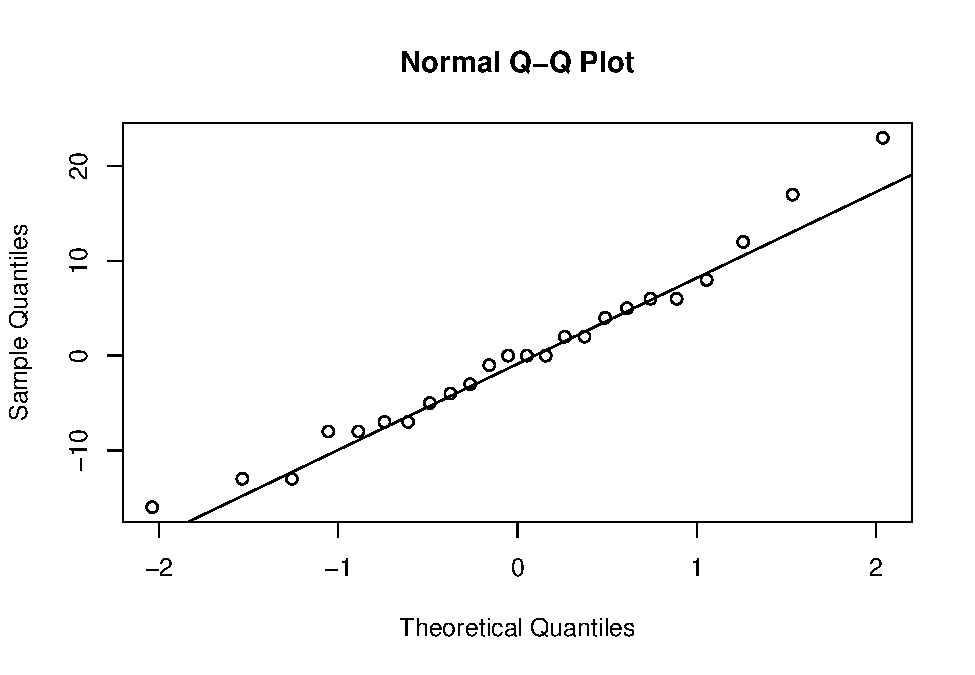
\includegraphics{05-OneWayANOVA_files/figure-latex/unnamed-chunk-11-1.pdf}

\begin{Shaded}
\begin{Highlighting}[]
\NormalTok{rij }\OtherTok{\textless{}{-}} \FunctionTok{rank}\NormalTok{(donuts}\SpecialCharTok{$}\NormalTok{y)}

\NormalTok{r1 }\OtherTok{\textless{}{-}} \FunctionTok{mean}\NormalTok{(rij[donuts}\SpecialCharTok{$}\NormalTok{Oil }\SpecialCharTok{==} \DecValTok{1}\NormalTok{])}
\NormalTok{r2 }\OtherTok{\textless{}{-}} \FunctionTok{mean}\NormalTok{(rij[donuts}\SpecialCharTok{$}\NormalTok{Oil}\SpecialCharTok{==} \DecValTok{2}\NormalTok{])}
\NormalTok{r3 }\OtherTok{\textless{}{-}} \FunctionTok{mean}\NormalTok{(rij[donuts}\SpecialCharTok{$}\NormalTok{Oil }\SpecialCharTok{==} \DecValTok{3}\NormalTok{])}
\NormalTok{r4 }\OtherTok{\textless{}{-}} \FunctionTok{mean}\NormalTok{(rij[donuts}\SpecialCharTok{$}\NormalTok{Oil }\SpecialCharTok{==} \DecValTok{4}\NormalTok{])}

\CommentTok{\# SSE}

\NormalTok{SSE }\OtherTok{\textless{}{-}} \FunctionTok{sum}\NormalTok{((rij[donuts}\SpecialCharTok{$}\NormalTok{Oil }\SpecialCharTok{==} \DecValTok{1}\NormalTok{] }\SpecialCharTok{{-}}\NormalTok{ r1)}\SpecialCharTok{\^{}}\DecValTok{2}\NormalTok{)}\SpecialCharTok{+}\FunctionTok{sum}\NormalTok{((rij[donuts}\SpecialCharTok{$}\NormalTok{Oil }\SpecialCharTok{==} \DecValTok{2}\NormalTok{] }\SpecialCharTok{{-}}\NormalTok{ r2)}\SpecialCharTok{\^{}}\DecValTok{2}\NormalTok{)}\SpecialCharTok{+}\FunctionTok{sum}\NormalTok{((rij[donuts}\SpecialCharTok{$}\NormalTok{Oil }\SpecialCharTok{==} \DecValTok{3}\NormalTok{] }\SpecialCharTok{{-}}\NormalTok{ r3)}\SpecialCharTok{\^{}}\DecValTok{2}\NormalTok{)}\SpecialCharTok{+}\FunctionTok{sum}\NormalTok{((rij[donuts}\SpecialCharTok{$}\NormalTok{Oil }\SpecialCharTok{==} \DecValTok{4}\NormalTok{] }\SpecialCharTok{{-}}\NormalTok{ r4)}\SpecialCharTok{\^{}}\DecValTok{2}\NormalTok{)}
\NormalTok{SSE}
\end{Highlighting}
\end{Shaded}

\begin{verbatim}
## [1] 557.4167
\end{verbatim}

\begin{Shaded}
\begin{Highlighting}[]
\NormalTok{SST }\OtherTok{\textless{}{-}} \FunctionTok{sum}\NormalTok{((rij }\SpecialCharTok{{-}} \FunctionTok{mean}\NormalTok{(rij))}\SpecialCharTok{\^{}}\DecValTok{2}\NormalTok{)}
\NormalTok{SST}
\end{Highlighting}
\end{Shaded}

\begin{verbatim}
## [1] 1148
\end{verbatim}

\begin{Shaded}
\begin{Highlighting}[]
\CommentTok{\# SSTr}
\NormalTok{SSTr }\OtherTok{\textless{}{-}}\NormalTok{ SST}\SpecialCharTok{{-}}\NormalTok{SSE}
\NormalTok{SSTr}
\end{Highlighting}
\end{Shaded}

\begin{verbatim}
## [1] 590.5833
\end{verbatim}

\begin{Shaded}
\begin{Highlighting}[]
\NormalTok{test.stat }\OtherTok{\textless{}{-}}\NormalTok{ (}\DecValTok{6}\SpecialCharTok{*}\DecValTok{4} \SpecialCharTok{{-}} \DecValTok{1}\NormalTok{)}\SpecialCharTok{*}\NormalTok{(SSTr }\SpecialCharTok{/}\NormalTok{ SST)}
\NormalTok{test.stat}
\end{Highlighting}
\end{Shaded}

\begin{verbatim}
## [1] 11.83224
\end{verbatim}

\begin{Shaded}
\begin{Highlighting}[]
\DecValTok{1}\SpecialCharTok{{-}}\FunctionTok{pchisq}\NormalTok{(test.stat, }\DecValTok{4{-}1}\NormalTok{)}
\end{Highlighting}
\end{Shaded}

\begin{verbatim}
## [1] 0.007980479
\end{verbatim}

\begin{Shaded}
\begin{Highlighting}[]
\FunctionTok{kruskal.test}\NormalTok{(y }\SpecialCharTok{\textasciitilde{}}\NormalTok{ Oil, }\AttributeTok{data =}\NormalTok{ donuts)}
\end{Highlighting}
\end{Shaded}

\begin{verbatim}
## 
##  Kruskal-Wallis rank sum test
## 
## data:  y by Oil
## Kruskal-Wallis chi-squared = 11.832, df = 3, p-value = 0.00798
\end{verbatim}

\hypertarget{randomized-complete-block-design}{%
\chapter{Randomized Complete Block Design}\label{randomized-complete-block-design}}

In this chapter we discuss the technique of \emph{blocking} which means to sample individuals from groups that are known (or strongly suspected) to have different average responses. Blocking is a type of explicit control---we account for the known effect of the blocks on the response through our sampling/experimental design. The effect of including blocks is (usually) to reduce the remaining variability in the response, thereby making it easier to detect treatment effects. One way to visualize this blocking effect is to recall the sum of squares decomposition SST = SSE + SSTr. When blocks are utilized, the decomposition becomes SST = SSE + SSBl + SSTr. The block sum of squares tends to absorb mostly the SSE term, thereby reducing the SSE and making the F ratio for treatments larger. However, some of the information of the data is ``used up'' estimating the block effects, and this reduces the degrees of freedom associated with MSE. Therefore, if ``useless'' blocks are used, we will tend to lose efficiency/power in detecting treatment effects.

\hypertarget{paired-experiments-as-blocking}{%
\section{Paired experiments as blocking}\label{paired-experiments-as-blocking}}

We are already familiar with blocking in a special type of two-sample experiment---paired data. For example, consider a paired design where responses on \(n\) individuals are measured as \(X_i\) ``before'' and \(Y_i\) ``after'' a treatment. The individuals constitute \(n\) blocks, with one sample, the difference \(D_i = Y_i - X_i\), for each block. The variance of \(D_i\) is \(V(D_i) = V(X_i) + V(Y_i) - 2Cov(X_i, Y_i)\). In a two-sample experiment where two different groups of individuals are treated, the covariance of responses between groups is zero. However, if multiple measurements are taken on the same individual, we generally expect the covariance of those measurements to be positive. Therefore, intuitively, we would expect the variance of differences of observations on the same individual to be lower than the variance of the difference of responses on two different individuals.

\hypertarget{randomized-complete-block-designs}{%
\section{Randomized Complete Block Designs}\label{randomized-complete-block-designs}}

\hypertarget{notation}{%
\subsection{Notation}\label{notation}}

We will use the following notation:
- \(n\) is the number of blocks
- \(J\) is the number of treatments
- \(r\) is the number of replications of each treatment in a block. So, each block has \(rJ\) responses.
- Y\_\{ijk\} is the response for the \(i^{th}\) block for treatment \(j\) at the \(k^{th}\) replicate.
- \(\overline Y_{i\cdot\cdot} = (rJ)^{-1}\sum_{j=1}^J\sum_{k=1}^r Y_{ijk}\) is the sample mean response of \(i^{th}\) block
- \(\overline Y_{\cdot j \cdot} = (rn)^{-1}\sum_{i=1}^n\sum_{k=1}^r Y_{ijk}\) is the sample mean response of \(j^{th}\) treatment
- \(\overline Y_{\cdot\cdot\cdot} = (rJn)^{-1}\sum_{i=1}^n\sum_{j=1}^J\sum_{k=1}^r Y_{ijk}\) is the sample mean response of all the responses, the grand sample mean.
In single replication studies, \(r=1\) and the third subscript is dropped from the notation.

The model may be written in the following effects-style notation:

\[Y_{ijk} = \mu + \beta_i + \tau_j + \epsilon_{ijk}\]

where \(\mu\) is an ``intercept'' term equal to \(E(Y_{ijk})\) if the other effects are actually zero; \(\beta_i\) for \(i=1, \ldots, n\) are the block effects, \(\tau_j\) for \(j = 1, \ldots, J\) are the treatment effects, and \(\epsilon_{ijk}\) is the effect of random sampling variability where \(\epsilon_{ijk}\stackrel{iid}{\sim}N(0,\sigma^2)\).

The above model requires two constraints in order to estimate the parameters \((\mu, \beta_i, \tau_j)\) for all \(i\) and \(j\). Here is the problem: the estimates of these parameters will be functions of the \(1 + n + J\) sample means above (the grand sample mean, block and treatment sample means). But, these are not all freely varying. For instance, since \(\overline Y_{\cdot\cdot\cdot} = (J)^{-1}\sum_{j=1}^J \overline Y_{\cdot j \cdot}\), it follows that we only need to know \(J-1\) of the \(J\) treatment sample means \(\overline Y_{\cdot j \cdot}\) and \(\overline Y_{\cdot\cdot\cdot}\) in order to determine the last one. The same is true of the block sample means. This means we must introduce two constraints on the parameters \((\mu, \beta_i, \tau_j)\) for all \(i\) and \(j\) to avoid defining parameters that are simply linear combinations of other parameters.

There are two common choices, the baseline constraints and the sum-to-zero constraints. Under the baseline constraints we set one of the treatment effects and one of the block effects to zero. Often, we would set \(\beta_n = 0\) and \(\tau_J = 0\), but sometimes (in some software) the first rather than last effects are set to zero. Whichever are set to zero are absorbed by \(\mu\) and \(\mu\) becomes the ``baseline'' effect. The remaining non-zero effects represent departures from the baseline. The second common constraint is the sum-to-zero constraint, which forces \(\sum \beta_i = \sum \tau_j = 0\). This constraint causes \(\mu\) to become the overall average response, and the effects to represent departures from the average.

\hypertarget{example-penicillin-manufacturing}{%
\subsection{Example: Penicillin Manufacturing}\label{example-penicillin-manufacturing}}

In this example 5 batches of raw organic material are used to make the antibiotic penicillin. We are interested in the yield of penicillin using 4 different industrial processes. Each process is used once per batch.

\begin{Shaded}
\begin{Highlighting}[]
\NormalTok{penicillin }\OtherTok{\textless{}{-}} \FunctionTok{read.csv}\NormalTok{(}\StringTok{\textquotesingle{}penicillin.csv\textquotesingle{}}\NormalTok{)}
\FunctionTok{head}\NormalTok{(penicillin)}
\end{Highlighting}
\end{Shaded}

\begin{verbatim}
##   Batch Process Yield
## 1     1       A    89
## 2     1       B    88
## 3     1       C    97
## 4     1       D    94
## 5     2       A    84
## 6     2       B    77
\end{verbatim}

\begin{Shaded}
\begin{Highlighting}[]
\NormalTok{penicillin}\SpecialCharTok{$}\NormalTok{Batch }\OtherTok{\textless{}{-}} \FunctionTok{factor}\NormalTok{(penicillin}\SpecialCharTok{$}\NormalTok{Batch, }\AttributeTok{levels =} \FunctionTok{unique}\NormalTok{(penicillin}\SpecialCharTok{$}\NormalTok{Batch))}
\NormalTok{penicillin}\SpecialCharTok{$}\NormalTok{Process }\OtherTok{\textless{}{-}} \FunctionTok{factor}\NormalTok{(penicillin}\SpecialCharTok{$}\NormalTok{Process, }\AttributeTok{levels =} \FunctionTok{unique}\NormalTok{(penicillin}\SpecialCharTok{$}\NormalTok{Process))}
\end{Highlighting}
\end{Shaded}

\begin{Shaded}
\begin{Highlighting}[]
\FunctionTok{boxplot}\NormalTok{(Yield }\SpecialCharTok{\textasciitilde{}}\NormalTok{ Process,}
        \AttributeTok{data =}\NormalTok{ penicillin)}
\end{Highlighting}
\end{Shaded}

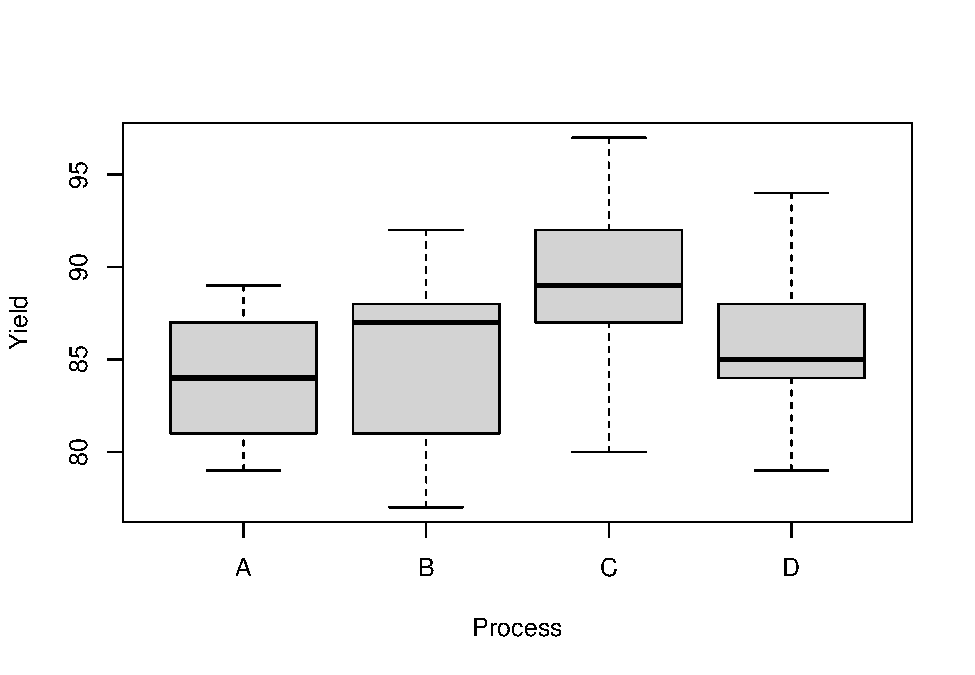
\includegraphics{06-RCBD_files/figure-latex/unnamed-chunk-3-1.pdf}

Let's see what parameter estimates R produces for the penicillin data. From the output of the lm function we see that treatment A and Batch 1 are missing---these are the baseline and are reflected in the intercept estimate, which is 90. How did R get 90? Well, the overall sample mean is 86; the process A mean yield is 84, and the batch 1 mean yield is 92. So, the effect of process A compared to the overall average is -2 and the effect of batch 1 compared to the overall average is +8. This combines for +6, so we end up with a batch1+processA baseline effect of 90 = 84+6. The rest of the effect estimates are easy to obtain as differences from this baseline. For example, since process B has a sample mean 1 larger than A, the process B effect is 1. And, since batch 3 has a sample mean effect 7 less than batch 1 the batch 3 effect is -7, and so on.

\begin{Shaded}
\begin{Highlighting}[]
\FunctionTok{library}\NormalTok{(tidyverse)}
\end{Highlighting}
\end{Shaded}

\begin{verbatim}
## -- Attaching packages --------------------------------------- tidyverse 1.3.2 --
## v ggplot2 3.3.6      v purrr   0.3.4 
## v tibble  3.1.8      v dplyr   1.0.10
## v tidyr   1.2.1      v stringr 1.4.1 
## v readr   2.1.2      v forcats 0.5.2 
## -- Conflicts ------------------------------------------ tidyverse_conflicts() --
## x dplyr::filter() masks stats::filter()
## x dplyr::lag()    masks stats::lag()
\end{verbatim}

\begin{Shaded}
\begin{Highlighting}[]
\NormalTok{by\_batch }\OtherTok{\textless{}{-}} \FunctionTok{group\_by}\NormalTok{(penicillin, Batch)}
\NormalTok{by\_batch }\OtherTok{\textless{}{-}} \FunctionTok{summarise}\NormalTok{(by\_batch, }\AttributeTok{batch\_mean =} \FunctionTok{mean}\NormalTok{(Yield))}
\NormalTok{by\_batch}
\end{Highlighting}
\end{Shaded}

\begin{verbatim}
## # A tibble: 5 x 2
##   Batch batch_mean
##   <fct>      <dbl>
## 1 1             92
## 2 2             83
## 3 3             85
## 4 4             88
## 5 5             82
\end{verbatim}

\begin{Shaded}
\begin{Highlighting}[]
\NormalTok{by\_trt }\OtherTok{\textless{}{-}} \FunctionTok{group\_by}\NormalTok{(penicillin, Process)}
\NormalTok{by\_trt }\OtherTok{\textless{}{-}} \FunctionTok{summarise}\NormalTok{(by\_trt, }\AttributeTok{trt\_mean =} \FunctionTok{mean}\NormalTok{(Yield))}
\NormalTok{by\_trt}
\end{Highlighting}
\end{Shaded}

\begin{verbatim}
## # A tibble: 4 x 2
##   Process trt_mean
##   <fct>      <dbl>
## 1 A             84
## 2 B             85
## 3 C             89
## 4 D             86
\end{verbatim}

\begin{Shaded}
\begin{Highlighting}[]
\FunctionTok{mean}\NormalTok{(penicillin}\SpecialCharTok{$}\NormalTok{Yield)}
\end{Highlighting}
\end{Shaded}

\begin{verbatim}
## [1] 86
\end{verbatim}

\begin{Shaded}
\begin{Highlighting}[]
\NormalTok{my.lm }\OtherTok{\textless{}{-}} \FunctionTok{lm}\NormalTok{(Yield}\SpecialCharTok{\textasciitilde{}}\NormalTok{Process}\SpecialCharTok{+}\NormalTok{Batch, }\AttributeTok{data =}\NormalTok{ penicillin)}
\FunctionTok{summary}\NormalTok{(my.lm)}
\end{Highlighting}
\end{Shaded}

\begin{verbatim}
## 
## Call:
## lm(formula = Yield ~ Process + Batch, data = penicillin)
## 
## Residuals:
##    Min     1Q Median     3Q    Max 
##  -5.00  -2.25  -0.50   2.25   6.00 
## 
## Coefficients:
##             Estimate Std. Error t value Pr(>|t|)    
## (Intercept)   90.000      2.745  32.791  4.1e-13 ***
## ProcessB       1.000      2.745   0.364  0.72194    
## ProcessC       5.000      2.745   1.822  0.09351 .  
## ProcessD       2.000      2.745   0.729  0.48018    
## Batch2        -9.000      3.069  -2.933  0.01254 *  
## Batch3        -7.000      3.069  -2.281  0.04159 *  
## Batch4        -4.000      3.069  -1.304  0.21686    
## Batch5       -10.000      3.069  -3.259  0.00684 ** 
## ---
## Signif. codes:  0 '***' 0.001 '**' 0.01 '*' 0.05 '.' 0.1 ' ' 1
## 
## Residual standard error: 4.34 on 12 degrees of freedom
## Multiple R-squared:  0.5964, Adjusted R-squared:  0.361 
## F-statistic: 2.534 on 7 and 12 DF,  p-value: 0.07535
\end{verbatim}

The \emph{options} statement below causes R to use the sum-to-zero constraints. We can see the resulting parameter estimates are now in terms of differences from the overall sample mean yield.

\begin{Shaded}
\begin{Highlighting}[]
\FunctionTok{options}\NormalTok{(}\AttributeTok{contrasts=}\FunctionTok{c}\NormalTok{(}\StringTok{\textquotesingle{}contr.sum\textquotesingle{}}\NormalTok{, }\StringTok{\textquotesingle{}contr.sum\textquotesingle{}}\NormalTok{))}
\NormalTok{my.lm.sum }\OtherTok{\textless{}{-}} \FunctionTok{lm}\NormalTok{(Yield}\SpecialCharTok{\textasciitilde{}}\NormalTok{Process}\SpecialCharTok{+}\NormalTok{Batch, }\AttributeTok{data =}\NormalTok{ penicillin)}
\FunctionTok{summary}\NormalTok{(my.lm.sum)}
\end{Highlighting}
\end{Shaded}

\begin{verbatim}
## 
## Call:
## lm(formula = Yield ~ Process + Batch, data = penicillin)
## 
## Residuals:
##    Min     1Q Median     3Q    Max 
##  -5.00  -2.25  -0.50   2.25   6.00 
## 
## Coefficients:
##             Estimate Std. Error t value Pr(>|t|)    
## (Intercept)  86.0000     0.9704  88.624  < 2e-16 ***
## Process1     -2.0000     1.6808  -1.190  0.25708    
## Process2     -1.0000     1.6808  -0.595  0.56292    
## Process3      3.0000     1.6808   1.785  0.09956 .  
## Batch1        6.0000     1.9408   3.092  0.00934 ** 
## Batch2       -3.0000     1.9408  -1.546  0.14812    
## Batch3       -1.0000     1.9408  -0.515  0.61573    
## Batch4        2.0000     1.9408   1.031  0.32310    
## ---
## Signif. codes:  0 '***' 0.001 '**' 0.01 '*' 0.05 '.' 0.1 ' ' 1
## 
## Residual standard error: 4.34 on 12 degrees of freedom
## Multiple R-squared:  0.5964, Adjusted R-squared:  0.361 
## F-statistic: 2.534 on 7 and 12 DF,  p-value: 0.07535
\end{verbatim}

We can obtain design matrices under both sets of constraints using the \emph{model.matrix} function. Note that the sum-to-zero design matrix literally has columns summing to zero!

\begin{Shaded}
\begin{Highlighting}[]
\NormalTok{X }\OtherTok{\textless{}{-}} \FunctionTok{model.matrix}\NormalTok{(my.lm)}
\NormalTok{X}
\end{Highlighting}
\end{Shaded}

\begin{verbatim}
##    (Intercept) ProcessB ProcessC ProcessD Batch2 Batch3 Batch4 Batch5
## 1            1        0        0        0      0      0      0      0
## 2            1        1        0        0      0      0      0      0
## 3            1        0        1        0      0      0      0      0
## 4            1        0        0        1      0      0      0      0
## 5            1        0        0        0      1      0      0      0
## 6            1        1        0        0      1      0      0      0
## 7            1        0        1        0      1      0      0      0
## 8            1        0        0        1      1      0      0      0
## 9            1        0        0        0      0      1      0      0
## 10           1        1        0        0      0      1      0      0
## 11           1        0        1        0      0      1      0      0
## 12           1        0        0        1      0      1      0      0
## 13           1        0        0        0      0      0      1      0
## 14           1        1        0        0      0      0      1      0
## 15           1        0        1        0      0      0      1      0
## 16           1        0        0        1      0      0      1      0
## 17           1        0        0        0      0      0      0      1
## 18           1        1        0        0      0      0      0      1
## 19           1        0        1        0      0      0      0      1
## 20           1        0        0        1      0      0      0      1
## attr(,"assign")
## [1] 0 1 1 1 2 2 2 2
## attr(,"contrasts")
## attr(,"contrasts")$Process
## [1] "contr.treatment"
## 
## attr(,"contrasts")$Batch
## [1] "contr.treatment"
\end{verbatim}

\begin{Shaded}
\begin{Highlighting}[]
\NormalTok{X }\OtherTok{\textless{}{-}} \FunctionTok{model.matrix}\NormalTok{(my.lm.sum)}
\NormalTok{X}
\end{Highlighting}
\end{Shaded}

\begin{verbatim}
##    (Intercept) Process1 Process2 Process3 Batch1 Batch2 Batch3 Batch4
## 1            1        1        0        0      1      0      0      0
## 2            1        0        1        0      1      0      0      0
## 3            1        0        0        1      1      0      0      0
## 4            1       -1       -1       -1      1      0      0      0
## 5            1        1        0        0      0      1      0      0
## 6            1        0        1        0      0      1      0      0
## 7            1        0        0        1      0      1      0      0
## 8            1       -1       -1       -1      0      1      0      0
## 9            1        1        0        0      0      0      1      0
## 10           1        0        1        0      0      0      1      0
## 11           1        0        0        1      0      0      1      0
## 12           1       -1       -1       -1      0      0      1      0
## 13           1        1        0        0      0      0      0      1
## 14           1        0        1        0      0      0      0      1
## 15           1        0        0        1      0      0      0      1
## 16           1       -1       -1       -1      0      0      0      1
## 17           1        1        0        0     -1     -1     -1     -1
## 18           1        0        1        0     -1     -1     -1     -1
## 19           1        0        0        1     -1     -1     -1     -1
## 20           1       -1       -1       -1     -1     -1     -1     -1
## attr(,"assign")
## [1] 0 1 1 1 2 2 2 2
## attr(,"contrasts")
## attr(,"contrasts")$Process
## [1] "contr.sum"
## 
## attr(,"contrasts")$Batch
## [1] "contr.sum"
\end{verbatim}

\hypertarget{sums-of-squares-and-f-tests-in-rcbd}{%
\subsection{Sums of squares and F tests in RCBD}\label{sums-of-squares-and-f-tests-in-rcbd}}

The primary goal of RCBD experiments is usually to evaluate whether all the treatment mean responses are equal, just as in one-way ANOVA. And, as in \emph{completely randomized experiments} --- experiments in which a random sample of experimental units are randomly assigned treatments --- an F test based on the ratio of two variance estimators is useful for testing this hypothesis. Keep in mind that we are not interested in testing whether the block mean responses are all equal, although we will consider a measure of the usefulness of blocking later on.

Just as in the completely randomized design, for RCBD experiments we can decompose the total sum of squares into components for blocks, treatments, and the ``errors'':

\begin{align*}
SST & = SSE + SSBl + SSTr\\
SST & = \sum_{i=1}^n\sum_{j=1}^J\sum_{k=1}^r (y_{ijk} - \overline y_{\cdot\cdot\cdot})^2\\
SSBl & = (rJ)\sum_{i=1}^n (\overline y_{i\cdot\cdot} - \overline y_{\cdot\cdot\cdot})^2\\
SSTr & = (rn)\sum_{j=1}^J (\overline y_{\cdot j\cdot} - \overline y_{\cdot\cdot\cdot})^2\\
SSE & = \sum_{i=1}^n\sum_{j=1}^J\sum_{k=1}^r (y_{ijk} -\overline y_{i\cdot\cdot}-\overline y_{\cdot j\cdot} + \overline y_{\cdot\cdot\cdot})^2
\end{align*}

To test the hypothesis \(H_0:\tau_j = 0, \,j=1, \ldots, J\), or equivalently, that the treatments have no effect (the mean response is constant over treatments) versus \(H_a:\text{ not all treatment effects are 0 }\), i.e., \(H_a: \tau_j\ne 0, \text{ for some }j\in \{1, \ldots, J\}\), we use the following F statistic:
\[F = \frac{SSTr/(J-1)}{SSE/(nJr - n - J +1)}\stackrel{H_0}{\sim} F_{J-1, nJr - n - J +1}.\]
To compute degrees of freedom of a sum of squares, the general rule is to subtract from the total number of summands the number of estimated parameters. For example, in SSTr there are J summands and 1 ``estimated parameter'', which is the parameter estimated by \(\overline y_{\cdot\cdot\cdot}\). And, in SSE there are \(nJr\) summands, and there are \(n+J+1-2\) uniquely determined sample means in the set \(\{\overline y_{1\cdot\cdot},\ldots, \overline y_{n\cdot\cdot}, \overline y_{\cdot 1\cdot}, \ldots, \overline y_{\cdot J\cdot},\overline y_{\cdot\cdot\cdot}\}\) as discussed above.

\hypertarget{example-significance-of-process-in-penicillin-experiment}{%
\subsection{Example: Significance of Process in Penicillin experiment}\label{example-significance-of-process-in-penicillin-experiment}}

The F test does not suggest mean yield varies over the four penicillin manufacturing processes.

\begin{Shaded}
\begin{Highlighting}[]
\NormalTok{SST }\OtherTok{\textless{}{-}} \FunctionTok{sum}\NormalTok{((penicillin}\SpecialCharTok{$}\NormalTok{Yield }\SpecialCharTok{{-}} \FunctionTok{mean}\NormalTok{(penicillin}\SpecialCharTok{$}\NormalTok{Yield))}\SpecialCharTok{\^{}}\DecValTok{2}\NormalTok{)}
\NormalTok{SSTr }\OtherTok{\textless{}{-}} \DecValTok{5}\SpecialCharTok{*}\FunctionTok{sum}\NormalTok{((by\_trt}\SpecialCharTok{$}\NormalTok{trt\_mean }\SpecialCharTok{{-}} \FunctionTok{mean}\NormalTok{(penicillin}\SpecialCharTok{$}\NormalTok{Yield))}\SpecialCharTok{\^{}}\DecValTok{2}\NormalTok{)}
\NormalTok{SSBl }\OtherTok{\textless{}{-}} \DecValTok{4}\SpecialCharTok{*}\FunctionTok{sum}\NormalTok{((by\_batch}\SpecialCharTok{$}\NormalTok{batch\_mean }\SpecialCharTok{{-}} \FunctionTok{mean}\NormalTok{(penicillin}\SpecialCharTok{$}\NormalTok{Yield))}\SpecialCharTok{\^{}}\DecValTok{2}\NormalTok{)}
\NormalTok{SSE }\OtherTok{\textless{}{-}}\NormalTok{ SST }\SpecialCharTok{{-}}\NormalTok{ SSTr }\SpecialCharTok{{-}}\NormalTok{ SSBl}
\NormalTok{SSTr}
\end{Highlighting}
\end{Shaded}

\begin{verbatim}
## [1] 70
\end{verbatim}

\begin{Shaded}
\begin{Highlighting}[]
\NormalTok{SSBl}
\end{Highlighting}
\end{Shaded}

\begin{verbatim}
## [1] 264
\end{verbatim}

\begin{Shaded}
\begin{Highlighting}[]
\NormalTok{SSE}
\end{Highlighting}
\end{Shaded}

\begin{verbatim}
## [1] 226
\end{verbatim}

\begin{Shaded}
\begin{Highlighting}[]
\NormalTok{F }\OtherTok{\textless{}{-}}\NormalTok{ (SSTr}\SpecialCharTok{/}\NormalTok{(}\DecValTok{4{-}1}\NormalTok{))}\SpecialCharTok{/}\NormalTok{(SSE }\SpecialCharTok{/}\NormalTok{ (}\DecValTok{5}\SpecialCharTok{*}\DecValTok{4{-}4{-}5}\SpecialCharTok{+}\DecValTok{1}\NormalTok{))}
\NormalTok{F}
\end{Highlighting}
\end{Shaded}

\begin{verbatim}
## [1] 1.238938
\end{verbatim}

\begin{Shaded}
\begin{Highlighting}[]
\DecValTok{1}\SpecialCharTok{{-}}\FunctionTok{pf}\NormalTok{(F,}\DecValTok{4{-}1}\NormalTok{,}\DecValTok{5}\SpecialCharTok{*}\DecValTok{4{-}4{-}5}\SpecialCharTok{+}\DecValTok{1}\NormalTok{)}
\end{Highlighting}
\end{Shaded}

\begin{verbatim}
## [1] 0.3386581
\end{verbatim}

\begin{Shaded}
\begin{Highlighting}[]
\NormalTok{my.aov }\OtherTok{\textless{}{-}} \FunctionTok{aov}\NormalTok{(Yield}\SpecialCharTok{\textasciitilde{}}\NormalTok{Batch}\SpecialCharTok{+}\NormalTok{Process, penicillin)}
\NormalTok{my.aov}
\end{Highlighting}
\end{Shaded}

\begin{verbatim}
## Call:
##    aov(formula = Yield ~ Batch + Process, data = penicillin)
## 
## Terms:
##                 Batch Process Residuals
## Sum of Squares    264      70       226
## Deg. of Freedom     4       3        12
## 
## Residual standard error: 4.339739
## Estimated effects may be unbalanced
\end{verbatim}

\begin{Shaded}
\begin{Highlighting}[]
\FunctionTok{summary}\NormalTok{(my.aov)}
\end{Highlighting}
\end{Shaded}

\begin{verbatim}
##             Df Sum Sq Mean Sq F value Pr(>F)  
## Batch        4    264   66.00   3.504 0.0407 *
## Process      3     70   23.33   1.239 0.3387  
## Residuals   12    226   18.83                 
## ---
## Signif. codes:  0 '***' 0.001 '**' 0.01 '*' 0.05 '.' 0.1 ' ' 1
\end{verbatim}

\hypertarget{follow-up-comparisons-and-contrasts}{%
\subsection{Follow-up comparisons and contrasts}\label{follow-up-comparisons-and-contrasts}}

Just as in one-way ANOVA for a completely randomized design (CRD) we may analyze pairwise comparisons of treatment mean responses when the F test rejects the hypothesis that all treatment means are the same. Or, we could estimate and test planned contrasts. And, there is essentially no differnce in how we apply these estimates and tests compared with CRD.

To compute Tukey HSD confidence intervals we use essentially the same formula:
\[\left(\overline Y_{i\cdot \cdot} - \overline Y_{\ell \cdot \cdot} \pm 2^{-1/2}q_{1-\alpha, \,J, \,nJr - n- J +1}\sqrt{MSE\left(\frac{1}{rn} + \frac{1}{rn}\right)}\right)\]
to define a set of simultaneous \(100(1-\alpha)\%\) CIs for the pairwise differences of treatment mean responses. (Recall \(q_{\alpha, \,u, \,v}\) is the \(\alpha\) quantile of Tukey's Studentized range distribution for \(u\) means and with \(v\) df.)

Let \(\gamma = c^\top \mu = \sum_{i=1}^J c_i \mu_i\) denote a linear combination of treatment mean responses where \(\sum_{i=1}^J c_i = 0\). Then, \(\gamma\) is a contrast, and
\[t = \frac{\hat\gamma - \gamma}{\sqrt{MSE\sum_{i=1}^J \left(\frac{c_i^2}{nr}\right)}}\sim t_{nrJ - n-J+1},\]
where \(\hat\gamma = \sum_{i=1}^J c_i \overline Y_{i\cdot\cdot}\). This \(t\) random variable may be used to derive point null hypothesis tests and CIs for \(\gamma\).

For simultaneous tests or CIs for a set of contrasts, we may use Scheff\textquotesingle e's method. The Scheff\textquotesingle e simultaneous \(100(1-\alpha)\%\) CIs for all linear contrasts are given by:
\[\left(\hat\gamma \pm \sqrt{(J-1)F_{1-\alpha, J-1, nJr-n-J+1}}\sqrt{MSE\sum_{i=1}^J \left(\frac{c_i^2}{nr}\right)}\right).\]

\hypertarget{example-tukey-contrasts-and-scheffe-for-penicillin-experiment}{%
\subsection{Example: Tukey, contrasts, and Scheffe for penicillin experiment}\label{example-tukey-contrasts-and-scheffe-for-penicillin-experiment}}

There is no reason to use Tukey's method with the penicillin experiment given the F test supports the null hypothesis. But, just for practice we can compute the Process B - Process A CI and compare with the built-in TukeyHSD function.

\begin{Shaded}
\begin{Highlighting}[]
\FunctionTok{c}\NormalTok{(by\_trt}\SpecialCharTok{$}\NormalTok{trt\_mean[}\DecValTok{2}\NormalTok{] }\SpecialCharTok{{-}}\NormalTok{ by\_trt}\SpecialCharTok{$}\NormalTok{trt\_mean[}\DecValTok{1}\NormalTok{] }\SpecialCharTok{{-}} \FunctionTok{sqrt}\NormalTok{(.}\DecValTok{5}\NormalTok{)}\SpecialCharTok{*}\FunctionTok{qtukey}\NormalTok{(}\FloatTok{0.95}\NormalTok{, }\DecValTok{4}\NormalTok{, }\DecValTok{4}\SpecialCharTok{*}\DecValTok{5{-}4{-}5}\SpecialCharTok{+}\DecValTok{1}\NormalTok{)}\SpecialCharTok{*}\FunctionTok{sqrt}\NormalTok{((SSE }\SpecialCharTok{/}\NormalTok{ (}\DecValTok{5}\SpecialCharTok{*}\DecValTok{4{-}4{-}5}\SpecialCharTok{+}\DecValTok{1}\NormalTok{))}\SpecialCharTok{*}\NormalTok{(}\DecValTok{2}\SpecialCharTok{/}\DecValTok{5}\NormalTok{)),}
\NormalTok{by\_trt}\SpecialCharTok{$}\NormalTok{trt\_mean[}\DecValTok{2}\NormalTok{] }\SpecialCharTok{{-}}\NormalTok{ by\_trt}\SpecialCharTok{$}\NormalTok{trt\_mean[}\DecValTok{1}\NormalTok{] }\SpecialCharTok{+} \FunctionTok{sqrt}\NormalTok{(.}\DecValTok{5}\NormalTok{)}\SpecialCharTok{*}\FunctionTok{qtukey}\NormalTok{(}\FloatTok{0.95}\NormalTok{, }\DecValTok{4}\NormalTok{, }\DecValTok{4}\SpecialCharTok{*}\DecValTok{5{-}4{-}5}\SpecialCharTok{+}\DecValTok{1}\NormalTok{)}\SpecialCharTok{*}\FunctionTok{sqrt}\NormalTok{((SSE }\SpecialCharTok{/}\NormalTok{ (}\DecValTok{5}\SpecialCharTok{*}\DecValTok{4{-}4{-}5}\SpecialCharTok{+}\DecValTok{1}\NormalTok{))}\SpecialCharTok{*}\NormalTok{(}\DecValTok{2}\SpecialCharTok{/}\DecValTok{5}\NormalTok{)))}
\end{Highlighting}
\end{Shaded}

\begin{verbatim}
## [1] -7.148719  9.148719
\end{verbatim}

\begin{Shaded}
\begin{Highlighting}[]
\FunctionTok{TukeyHSD}\NormalTok{(my.aov, }\AttributeTok{which =} \StringTok{\textquotesingle{}Process\textquotesingle{}}\NormalTok{)}
\end{Highlighting}
\end{Shaded}

\begin{verbatim}
##   Tukey multiple comparisons of means
##     95% family-wise confidence level
## 
## Fit: aov(formula = Yield ~ Batch + Process, data = penicillin)
## 
## $Process
##     diff        lwr       upr     p adj
## B-A    1  -7.148719  9.148719 0.9826684
## C-A    5  -3.148719 13.148719 0.3105094
## D-A    2  -6.148719 10.148719 0.8837551
## C-B    4  -4.148719 12.148719 0.4905194
## D-B    1  -7.148719  9.148719 0.9826684
## D-C   -3 -11.148719  5.148719 0.7002271
\end{verbatim}

Next, let's test is the Process C mean yield is different than the average of the other processes. This is a contrast with \(c = (-1/3,-1/3,1,-1/3)\). We might be tempted to test this particular contrast after peeking at the boxplot above. That's not a good idea! Using the data to suggest tests to perform leads to inflated Type 1 errors. However, if we apply Scheff\textquotesingle e's correction, then we control the Type 1 error rate for all linear contrasts, which includes comparisons that are \emph{inspired} by the data.

At \(\alpha = .10\) we would actually reject the null hypothesis that the Process C mean is equal to the average of the A, B, and D means if we performed the uncorrected test (which we should not because we chose to based on the boxplot). But, the Scheff\textquotesingle e correction saves us from our shameful p-value snooping!

\begin{Shaded}
\begin{Highlighting}[]
\NormalTok{hat.gamma }\OtherTok{\textless{}{-}}\NormalTok{ by\_trt}\SpecialCharTok{$}\NormalTok{trt\_mean[}\DecValTok{3}\NormalTok{] }\SpecialCharTok{{-}} \FunctionTok{mean}\NormalTok{(}\FunctionTok{c}\NormalTok{(by\_trt}\SpecialCharTok{$}\NormalTok{trt\_mean[}\FunctionTok{c}\NormalTok{(}\DecValTok{1}\NormalTok{,}\DecValTok{2}\NormalTok{,}\DecValTok{4}\NormalTok{)]))}
\NormalTok{t }\OtherTok{\textless{}{-}}\NormalTok{ hat.gamma }\SpecialCharTok{/} \FunctionTok{sqrt}\NormalTok{((SSE }\SpecialCharTok{/}\NormalTok{ (}\DecValTok{5}\SpecialCharTok{*}\DecValTok{4{-}4{-}5}\SpecialCharTok{+}\DecValTok{1}\NormalTok{)) }\SpecialCharTok{*}\NormalTok{ (}\DecValTok{1}\SpecialCharTok{/}\DecValTok{5} \SpecialCharTok{+} \DecValTok{3}\SpecialCharTok{*}\NormalTok{(}\DecValTok{1}\SpecialCharTok{/}\NormalTok{(}\DecValTok{5}\SpecialCharTok{*}\DecValTok{9}\NormalTok{))))}
\DecValTok{2}\SpecialCharTok{*}\NormalTok{(}\DecValTok{1}\SpecialCharTok{{-}}\FunctionTok{pt}\NormalTok{(}\FunctionTok{abs}\NormalTok{(t), }\DecValTok{5}\SpecialCharTok{*}\DecValTok{4{-}4{-}5}\SpecialCharTok{+}\DecValTok{1}\NormalTok{)) }\CommentTok{\# uncorrected p{-}value}
\end{Highlighting}
\end{Shaded}

\begin{verbatim}
## [1] 0.09955857
\end{verbatim}

\begin{Shaded}
\begin{Highlighting}[]
\NormalTok{F }\OtherTok{\textless{}{-}}\NormalTok{ (t}\SpecialCharTok{/}\FunctionTok{sqrt}\NormalTok{(}\DecValTok{4{-}1}\NormalTok{))}\SpecialCharTok{\^{}}\DecValTok{2}
\DecValTok{1}\SpecialCharTok{{-}}\FunctionTok{pf}\NormalTok{(F, }\DecValTok{4{-}1}\NormalTok{, }\DecValTok{5}\SpecialCharTok{*}\DecValTok{4{-}4{-}5}\SpecialCharTok{+}\DecValTok{1}\NormalTok{) }\CommentTok{\# Scheffe corrected p{-}value}
\end{Highlighting}
\end{Shaded}

\begin{verbatim}
## [1] 0.4014427
\end{verbatim}

\begin{Shaded}
\begin{Highlighting}[]
\FunctionTok{library}\NormalTok{(emmeans) }
\NormalTok{fit.emm }\OtherTok{\textless{}{-}} \FunctionTok{emmeans}\NormalTok{(my.aov, }\StringTok{"Process"}\NormalTok{)}
\CommentTok{\# unadjusted, just testing one contrast}
\FunctionTok{summary}\NormalTok{(}\FunctionTok{contrast}\NormalTok{(fit.emm, }\AttributeTok{method =} \FunctionTok{list}\NormalTok{(}\FunctionTok{c}\NormalTok{(}\SpecialCharTok{{-}}\DecValTok{1}\SpecialCharTok{/}\DecValTok{3}\NormalTok{, }\SpecialCharTok{{-}}\DecValTok{1}\SpecialCharTok{/}\DecValTok{3}\NormalTok{, }\DecValTok{1}\NormalTok{,}\SpecialCharTok{{-}}\DecValTok{1}\SpecialCharTok{/}\DecValTok{3}\NormalTok{))))}
\end{Highlighting}
\end{Shaded}

\begin{verbatim}
##  contrast                                                        estimate   SE
##  c(-0.333333333333333, -0.333333333333333, 1, -0.333333333333333        4 2.24
##  df t.ratio p.value
##  12   1.785  0.0996
## 
## Results are averaged over the levels of: Batch
\end{verbatim}

\begin{Shaded}
\begin{Highlighting}[]
\CommentTok{\# Scheffe adjustment so that we could test all linear contrasts}
\FunctionTok{summary}\NormalTok{(}\FunctionTok{contrast}\NormalTok{(fit.emm, }\AttributeTok{method =} \FunctionTok{list}\NormalTok{(}\FunctionTok{c}\NormalTok{(}\SpecialCharTok{{-}}\DecValTok{1}\SpecialCharTok{/}\DecValTok{3}\NormalTok{, }\SpecialCharTok{{-}}\DecValTok{1}\SpecialCharTok{/}\DecValTok{3}\NormalTok{, }\DecValTok{1}\NormalTok{,}\SpecialCharTok{{-}}\DecValTok{1}\SpecialCharTok{/}\DecValTok{3}\NormalTok{)), }
                 \AttributeTok{adjust =} \StringTok{"scheffe"}\NormalTok{), }\AttributeTok{scheffe.rank =} \DecValTok{3}\NormalTok{)}
\end{Highlighting}
\end{Shaded}

\begin{verbatim}
##  contrast                                                        estimate   SE
##  c(-0.333333333333333, -0.333333333333333, 1, -0.333333333333333        4 2.24
##  df t.ratio p.value
##  12   1.785  0.4014
## 
## Results are averaged over the levels of: Batch 
## P value adjustment: scheffe method with rank 3
\end{verbatim}

\hypertarget{relative-efficiency-of-blocking-vs.-crd}{%
\subsection{Relative efficiency of Blocking (vs.~CRD)}\label{relative-efficiency-of-blocking-vs.-crd}}

After an RCBD experiment is performed it is sometimes helpful for researchers to understand whether blocking was a helpful part of the experimental design. Blocking variables are selected by the researchers with the belief their levels are associated with different average responses. The idea is that if we take into account the variability in response due to block variable levels, we will reduce the unexplained variability. This manifests in the decomposition
\[SST = SSE + SSBl + SSTr\]
where we expect the block sum of squares to ``absorb'' part of the SSE that would have been present in a CRD. Smaller SSE in turn increases the F statistic \(F = MSTr/MSE\) for testing significance of the treatments by lowering the denominator in the ratio. On the other hand, blocking creates an opposite effect that decreases this F statistic as well. Just like the total sum of squares decomposes, so do the degrees of freedom:
\[nJr - 1 = (nJr - n - J + 1) + (n-1) + (J-1).\]
The upshot is that the number of degrees of freedom ``used'' in estimating SSE is smaller if blocks are included compared to a CRD with no blocks and equal total sample size. This reduces the denominator of MSE, which increases MSE relative to CRD and thus decreases the F ratio for testing for significant treatment effects. Usually, if experimenters choose a small number of intuitively useful blocks, RCBD is ``more efficient'' than CRD in the sense that its F test has increased power to detect treatment effects.

We can attempt to quantify the effect of blocking compared to CRD using a post-experiment measure called the relative efficiency (RE) of blocking (relative, that is, to CRD). The formula, given below, accounts for both the decrease in degrees of freedom and the approximate decrease in \(\hat\sigma^2\) when blocking (RCBD) versus not blocking (CRD):
\[RE = \frac{df_{MSE,RCBD} + 1}{df_{MSE,CRD} + 1}\frac{df_{MSE,CRD} + 3}{df_{MSE,RCBD} + 3}\frac{\hat\sigma^2_{CRD}}{\hat\sigma^2_{RCBD}},\]
where
\[\hat\sigma^2_{CRD} = MSE_{CRD},\]
\[MSE_{CRD} = \frac{df_{Bl}MSBl_{RCBD} + (df_{Tr}+df_{E})MSE_{RCBD}}{df_{Bl} + df_{Tr} + df_E}.\]
And, from above, we have
\[df_{Tr} = J-1, \quad df_{Bl} = n-1, \quad df_{E} = df_{MSE,RCBD} = nJr - n - J +1, \quad \text{and    }\, df_{MSE,CRD} = nJr - J.\]

\hypertarget{example-re-of-blocking-in-penicillin-experiment}{%
\subsection{Example: RE of blocking in penicillin experiment}\label{example-re-of-blocking-in-penicillin-experiment}}

The relative efficiency of blocking is about 1.48, which can be interpreted as saying each replicated response in the RCBD experiment provides approximately 1.48 times at much (\(48\%\) more) information compared to a replicate in a CRD design. In other words, it would take \(48\%\) more samples in a CRD to get the same amount of information as in a RCBD. As long as RE is above 1, the RCBD design provides an advantage over CRD. Since it may be substantially more work to implement a RCBD than a CRD, experimenters would like to see a substantial advantage in RE for RCBD relative to CRD.

\begin{Shaded}
\begin{Highlighting}[]
\NormalTok{MSE\_RCBD }\OtherTok{\textless{}{-}}\NormalTok{ SSE }\SpecialCharTok{/}\NormalTok{ (}\DecValTok{4}\SpecialCharTok{*}\DecValTok{5{-}4{-}5}\SpecialCharTok{+}\DecValTok{1}\NormalTok{)}
\NormalTok{MSBl }\OtherTok{\textless{}{-}}\NormalTok{ SSBl }\SpecialCharTok{/}\NormalTok{ (}\DecValTok{5{-}1}\NormalTok{)}
\NormalTok{MSE\_CRD }\OtherTok{\textless{}{-}}\NormalTok{ ((}\DecValTok{5{-}1}\NormalTok{)}\SpecialCharTok{*}\NormalTok{MSBl }\SpecialCharTok{+}\NormalTok{ (}\DecValTok{5}\SpecialCharTok{*}\DecValTok{4{-}5{-}4}\SpecialCharTok{+}\DecValTok{1} \SpecialCharTok{+} \DecValTok{4{-}1}\NormalTok{)}\SpecialCharTok{*}\NormalTok{MSE\_RCBD)}\SpecialCharTok{/}\NormalTok{(}\DecValTok{5}\SpecialCharTok{*}\DecValTok{4{-}5{-}4}\SpecialCharTok{+}\DecValTok{1}\SpecialCharTok{+}\DecValTok{4{-}1}\SpecialCharTok{+}\DecValTok{5{-}1}\NormalTok{)}
\NormalTok{df\_MSE\_CRD }\OtherTok{\textless{}{-}} \DecValTok{5}\SpecialCharTok{*}\DecValTok{4{-}4}
\NormalTok{df\_MSE\_RCBD }\OtherTok{\textless{}{-}} \DecValTok{5}\SpecialCharTok{*}\DecValTok{4{-}4{-}5}\SpecialCharTok{+}\DecValTok{1}

\NormalTok{RE }\OtherTok{\textless{}{-}}\NormalTok{ (MSE\_CRD}\SpecialCharTok{/}\NormalTok{MSE\_RCBD) }\SpecialCharTok{*}\NormalTok{ ((df\_MSE\_CRD}\SpecialCharTok{+}\DecValTok{3}\NormalTok{)}\SpecialCharTok{/}\NormalTok{(df\_MSE\_RCBD }\SpecialCharTok{+}\DecValTok{3}\NormalTok{)) }\SpecialCharTok{*}\NormalTok{ ((df\_MSE\_RCBD}\SpecialCharTok{+}\DecValTok{1}\NormalTok{)}\SpecialCharTok{/}\NormalTok{(df\_MSE\_CRD }\SpecialCharTok{+}\DecValTok{1}\NormalTok{))}
\NormalTok{RE}
\end{Highlighting}
\end{Shaded}

\begin{verbatim}
## [1] 1.479334
\end{verbatim}

\hypertarget{latin-squares-for-two-blocking-variables}{%
\chapter{Latin Squares for two blocking variables}\label{latin-squares-for-two-blocking-variables}}

\hypertarget{designs-for-multiple-blocks}{%
\section{Designs for multiple blocks}\label{designs-for-multiple-blocks}}

Suppose we have two blocking variables and one treatment variable, and suppose all three of these categorical variables have the same number of levels. For example, suppose an experiment to measure the miles per gallon (MPG) of automobiles using 4 types of gasoline fuel additives (the treatments) is blocked by 4 models of car and 4 different drivers driving the cars on the same road course. In order to carry out an RCBD we would consider the 16 crossed blocks given by driver times car model. And, we require each treatment to be replicated at least once per block, which means we need a total of at least 64 samples.

The Latin square design is a special design for the case of 2 (or more) blocking variables and one treatment variable all having the same number of levels. The Latin square (or cube, or hypercube!) only requires one treatment be used for each combination of blocks, but according to a strict pattern: If we write down a grid or matrix corresponding to crossing the levels of the two blocking variables, then a Latin square design corresponds to every treatment level appearing in each row and column exactly once (think of a sudoku puzzle).

\hypertarget{example-mpg-experiment}{%
\subsection{Example: MPG experiment}\label{example-mpg-experiment}}

Four for drivers (1,2,3,4), four cars (1,2,3,4), and four treatments/additives (A,B,C,D) we have the following Latin square design:

\begin{longtable}[]{@{}llllll@{}}
\toprule()
& & Driver & & & \\
\midrule()
\endhead
& & 1 & 2 & 3 & 4 \\
Car & 1 & A & B & C & D \\
& 2 & B & C & D & A \\
& 3 & C & D & A & B \\
& 4 & D & A & B & C \\
\bottomrule()
\end{longtable}

\hypertarget{model-notation}{%
\section{Model notation}\label{model-notation}}

A Latin square design may be represented by the follwowing model:
\[Y_{ijk} = \mu + \beta_i + \gamma_j + \tau_k + \epsilon_{ijk}\]
where \(i, j, k = 1, \ldots, r\), \(\beta\) and \(\gamma\) refer to row and column block effects and \(\tau\) is the treatment effect. As always, the model is over-parametrized, and constraints are necessary; for example, the baseline constraint \(\beta_r = \gamma_r = \tau_r = 0\).

\hypertarget{sums-of-squares-and-test-for-treatment-effects}{%
\section{Sums of squares and test for treatment effects}\label{sums-of-squares-and-test-for-treatment-effects}}

The row (SSBr) and column (SSBc) block sums of squares, and treatment (SSTr) sums of squares are given by:
\[SSBr = r\sum_{i}(\overline Y_{i\cdot\cdot} - \overline Y_{\cdot\cdot\cdot})^2, \quad SSBc = r\sum_{j}(\overline Y_{\cdot j\cdot} - \overline Y_{\cdot\cdot\cdot})^2, \quad SSBr = r\sum_{k}(\overline Y_{\cdot\cdot k} - \overline Y_{\cdot\cdot\cdot})^2.\]
Each have \(r-1\) degrees of freedom (r summands minus 1 estimated parameter, which is \(\overline Y_{\cdot\cdot\cdot}\) estimating the overall mean parameter). The total sum of squares is
\[SST = \sum_i\sum_j\sum_k(Y_{ijk} - \overline{Y}_{\cdot\cdot\cdot})^2\]
which has \(r^2 - 1\) degrees of freedom (\(r^2\) summands minus one estimated parameter, which is \(\overline Y_{\cdot\cdot\cdot}\) estimating the overall mean parameter). The SSE is most easily obtained by subtraction:
\[SSE = SST - SSBr - SSBc - SSTr\]
and has degrees of freedom (obtained by subtraction) \((r-1)(r-2)\).

The most important test is the test for significant treatments: \(H_0: \tau_k = 0, \text{for all } k\) versus \(H_a: \text{ at least one treatment has an effect}\) on the mean response.

\hypertarget{example-mpg-experiment-1}{%
\subsection{Example: MPG experiment}\label{example-mpg-experiment-1}}

The following MPG measurements were obtained using a Latin square design.

\begin{longtable}[]{@{}llllll@{}}
\toprule()
& & Driver & & & \\
\midrule()
\endhead
& & 1 & 2 & 3 & 4 \\
Car & 1 & A = 24 & B = 26 & C = 16 & D = 20 \\
& 2 & B = 15 & C = 26 & D = 20 & A = 16 \\
& 3 & C = 17 & D = 13 & A = 20 & B = 27 \\
& 4 & D = 23 & A = 15 & B = 20 & C = 25 \\
\bottomrule()
\end{longtable}

\begin{Shaded}
\begin{Highlighting}[]
\NormalTok{mpg }\OtherTok{\textless{}{-}} \FunctionTok{data.frame}\NormalTok{(}\AttributeTok{car =} \FunctionTok{c}\NormalTok{(}\DecValTok{1}\NormalTok{,}\DecValTok{2}\NormalTok{,}\DecValTok{3}\NormalTok{,}\DecValTok{4}\NormalTok{,}\DecValTok{1}\NormalTok{,}\DecValTok{2}\NormalTok{,}\DecValTok{3}\NormalTok{,}\DecValTok{4}\NormalTok{,}\DecValTok{1}\NormalTok{,}\DecValTok{2}\NormalTok{,}\DecValTok{3}\NormalTok{,}\DecValTok{4}\NormalTok{,}\DecValTok{1}\NormalTok{,}\DecValTok{2}\NormalTok{,}\DecValTok{3}\NormalTok{,}\DecValTok{4}\NormalTok{), }\AttributeTok{driver =} \FunctionTok{c}\NormalTok{(}\DecValTok{1}\NormalTok{,}\DecValTok{1}\NormalTok{,}\DecValTok{1}\NormalTok{,}\DecValTok{1}\NormalTok{,}\DecValTok{2}\NormalTok{,}\DecValTok{2}\NormalTok{,}\DecValTok{2}\NormalTok{,}\DecValTok{2}\NormalTok{,}\DecValTok{3}\NormalTok{,}\DecValTok{3}\NormalTok{,}\DecValTok{3}\NormalTok{,}\DecValTok{3}\NormalTok{,}\DecValTok{4}\NormalTok{,}\DecValTok{4}\NormalTok{,}\DecValTok{4}\NormalTok{,}\DecValTok{4}\NormalTok{), }\AttributeTok{additive =} \FunctionTok{c}\NormalTok{(}\StringTok{\textquotesingle{}A\textquotesingle{}}\NormalTok{, }\StringTok{\textquotesingle{}B\textquotesingle{}}\NormalTok{, }\StringTok{\textquotesingle{}C\textquotesingle{}}\NormalTok{,}\StringTok{\textquotesingle{}D\textquotesingle{}}\NormalTok{,}\StringTok{\textquotesingle{}B\textquotesingle{}}\NormalTok{,}\StringTok{\textquotesingle{}C\textquotesingle{}}\NormalTok{,}\StringTok{\textquotesingle{}D\textquotesingle{}}\NormalTok{,}\StringTok{\textquotesingle{}A\textquotesingle{}}\NormalTok{,}\StringTok{\textquotesingle{}C\textquotesingle{}}\NormalTok{,}\StringTok{\textquotesingle{}D\textquotesingle{}}\NormalTok{,}\StringTok{\textquotesingle{}A\textquotesingle{}}\NormalTok{,}\StringTok{\textquotesingle{}B\textquotesingle{}}\NormalTok{,}\StringTok{\textquotesingle{}D\textquotesingle{}}\NormalTok{,}\StringTok{\textquotesingle{}A\textquotesingle{}}\NormalTok{,}\StringTok{\textquotesingle{}B\textquotesingle{}}\NormalTok{,}\StringTok{\textquotesingle{}C\textquotesingle{}}\NormalTok{), }\AttributeTok{mpg =} \FunctionTok{c}\NormalTok{(}\DecValTok{24}\NormalTok{,}\DecValTok{15}\NormalTok{,}\DecValTok{17}\NormalTok{,}\DecValTok{23}\NormalTok{,}\DecValTok{26}\NormalTok{,}\DecValTok{26}\NormalTok{,}\DecValTok{13}\NormalTok{,}\DecValTok{15}\NormalTok{,}\DecValTok{16}\NormalTok{,}\DecValTok{20}\NormalTok{,}\DecValTok{20}\NormalTok{,}\DecValTok{20}\NormalTok{,}\DecValTok{20}\NormalTok{,}\DecValTok{16}\NormalTok{,}\DecValTok{27}\NormalTok{,}\DecValTok{25}\NormalTok{) )}
\NormalTok{mpg}\SpecialCharTok{$}\NormalTok{car }\OtherTok{\textless{}{-}} \FunctionTok{factor}\NormalTok{(mpg}\SpecialCharTok{$}\NormalTok{car, }\AttributeTok{levels =} \FunctionTok{unique}\NormalTok{(mpg}\SpecialCharTok{$}\NormalTok{car))}
\NormalTok{mpg}\SpecialCharTok{$}\NormalTok{driver }\OtherTok{\textless{}{-}} \FunctionTok{factor}\NormalTok{(mpg}\SpecialCharTok{$}\NormalTok{driver, }\AttributeTok{levels =} \FunctionTok{unique}\NormalTok{(mpg}\SpecialCharTok{$}\NormalTok{driver))}
\NormalTok{mpg}\SpecialCharTok{$}\NormalTok{additive }\OtherTok{\textless{}{-}} \FunctionTok{factor}\NormalTok{(mpg}\SpecialCharTok{$}\NormalTok{additive, }\AttributeTok{levels =} \FunctionTok{unique}\NormalTok{(mpg}\SpecialCharTok{$}\NormalTok{additive))}

\NormalTok{my.aov }\OtherTok{\textless{}{-}} \FunctionTok{aov}\NormalTok{(mpg}\SpecialCharTok{\textasciitilde{}}\NormalTok{additive }\SpecialCharTok{+}\NormalTok{ car}\SpecialCharTok{+}\NormalTok{driver, }\AttributeTok{data =}\NormalTok{ mpg)}
\FunctionTok{summary}\NormalTok{(my.aov)}
\end{Highlighting}
\end{Shaded}

\begin{verbatim}
##             Df Sum Sq Mean Sq F value Pr(>F)
## additive     3  29.69    9.90   0.241  0.865
## car          3  15.19    5.06   0.124  0.943
## driver       3  19.69    6.56   0.160  0.919
## Residuals    6 245.87   40.98
\end{verbatim}

\hypertarget{relative-efficiency-of-blocking}{%
\section{Relative efficiency of blocking}\label{relative-efficiency-of-blocking}}

The efficiency of a Latin square design may be assessed relative to a CRD or an RCBD using only the row or only the column blocking variable. For comparison to and RCBD using the row block, we have the formula:

\[RE = \frac{MSE_{row}}{MSE_{LS}} \times \text{df correction}\]
where \(MSE_{row} = \frac{MS_{row} + (r-1)MSE_{LS}}{r}\), where \(MSE_{LS}\) denotes the observed MSE from the Latin square experiment, \(MS_{row}\) denotes the oserved mean sum of squares of the row blocking variable from the Latin square experiment, and where
\[\text{df correction} = \frac{df_{E, LS}+1}{df_{E,RCBD} + 1}\times\frac{df_{E,RCBD}+3}{df_{E,LS}+3} = \frac{r^2-3r+3}{r^2-2r+2}\times\frac{r^2-2r+4}{r^2-3r+5}.\]

\hypertarget{example-re-ignoring-driver-blocks}{%
\subsection{Example: RE ignoring driver blocks}\label{example-re-ignoring-driver-blocks}}

Neither blocking variable was particularly helpful. The RE relative to RCBD without driver is only about \(74\%\).

\begin{Shaded}
\begin{Highlighting}[]
\NormalTok{MSE\_row }\OtherTok{\textless{}{-}}\NormalTok{ (}\FloatTok{6.56} \SpecialCharTok{+} \DecValTok{3}\SpecialCharTok{*}\FloatTok{40.98}\NormalTok{)}\SpecialCharTok{/}\DecValTok{4}
\NormalTok{correction }\OtherTok{\textless{}{-}} \ControlFlowTok{function}\NormalTok{(r)  (r}\SpecialCharTok{\^{}}\DecValTok{2} \SpecialCharTok{{-}} \DecValTok{3}\SpecialCharTok{*}\NormalTok{r}\SpecialCharTok{+}\DecValTok{3}\NormalTok{)}\SpecialCharTok{*}\NormalTok{(r}\SpecialCharTok{\^{}}\DecValTok{2} \SpecialCharTok{{-}} \DecValTok{2}\SpecialCharTok{*}\NormalTok{r}\SpecialCharTok{+}\DecValTok{4}\NormalTok{)}\SpecialCharTok{/}\NormalTok{((r}\SpecialCharTok{\^{}}\DecValTok{2{-}3}\SpecialCharTok{*}\NormalTok{r}\SpecialCharTok{+}\DecValTok{5}\NormalTok{)}\SpecialCharTok{*}\NormalTok{(r}\SpecialCharTok{\^{}}\DecValTok{2} \SpecialCharTok{{-}} \DecValTok{2}\SpecialCharTok{*}\NormalTok{r}\SpecialCharTok{+}\DecValTok{2}\NormalTok{))}
\NormalTok{RE }\OtherTok{\textless{}{-}}\NormalTok{ (MSE\_row }\SpecialCharTok{/} \FloatTok{40.98}\NormalTok{)}\SpecialCharTok{*}\FunctionTok{correction}\NormalTok{(}\DecValTok{4}\NormalTok{)}
\NormalTok{RE}
\end{Highlighting}
\end{Shaded}

\begin{verbatim}
## [1] 0.7373516
\end{verbatim}

\hypertarget{two-way-anova}{%
\chapter{Two-Way ANOVA}\label{two-way-anova}}

Two-way ANOVA models represent experiments with two categorical treatment variables and aim to quantify uncertainty about differences in mean response over the levels of these treatments. Superficially, these models appear similar to RCBDs, but neither categorical variable is a block, rather, the effects of both on the response are of interest. We could simply cross the levels of the two treatments and perform a one-way ANOVA, but that will make it challenging to sort out which treatment variable drives the differences in mean response. If we were to apply Tukey tests afterwards, we would have difficulties interpreting comparisons of different levels of different treatment variables. The main advantage of the two-way setup is the presence of explicit ``interaction'' effects for the crossed treatments. If these are insignificant in their effects on the mean response, then the model is simply additive, i.e., the effects of the two treatments are separable and therefore easily interpretable.

\hypertarget{the-model}{%
\section{The Model}\label{the-model}}

Let \(i = 1, \ldots, a\) denote the number of levels of treatment variable A, \(j = 1, \ldots, b\) denote the same for treatment variable B, and let \(k = 1, \ldots, n\) denote the number of replications at each pair of crossed levels. We consider only balanced designs (for now). Then, the effects model may be written
\[Y_{ijk} = \mu + \alpha_i + \beta_j + (\alpha\beta)_{ij} + \epsilon_{ijk}\]
where \(\alpha_i\) and \(\beta_j\) are the ``main effects'' parameters for the treatment variables A and B and the \((\alpha\beta)_{ij}\) parameters are ``interaction'' effects representing synergistic effects between the two treatment variables---in other words, allowing for the treatment effects to be non-additive. As written, the model contains too many parameters---there are 1 + a + b + ab for a total of ab crossed treatment mean responses. So, we need 1+a+b constraints. One choice is the baseline constraints in which we set \(\alpha_a = \beta_b = (\alpha\beta)_{i,b} = (\alpha\beta)_{a,j} = 0\). This zeroes out \(1+1+a+b-1\) parameters. (Note, there is a redundancy because \(((\alpha\beta)_{a,b})\) appears twice in the constraint set, hence the minus 1.) It is also possible to specify sum-to-zero constraints.

\hypertarget{example-protein-chemistry}{%
\subsection{Example: protein chemistry}\label{example-protein-chemistry}}

An experiment is done in which minnows are fed diets with different amounts of zinc and copper supplements. The experimenters record the protein content of the minnows once harvested. Let the levels of copper be 0 and 100 and for zinc be 0, 100 and 200. Then, there are 6 treatment mean responses. Using the baseline constraint, we have the parameters \(\mu, \alpha_1, \beta_1, \beta_2, (\alpha\beta)_{11}, (\alpha\beta)_{12}\).

\hypertarget{tests-for-interaction-and-main-effects}{%
\section{Tests for interaction and main effects}\label{tests-for-interaction-and-main-effects}}

The most important questions to be answered are: ``do the treatments effect the mean response?'' and ``are those effects separable/additive?'' We may answer these questions using tests of interaction and main effects.
The test for interaction has null hypothesis \(H_0: (\alpha\beta)_{ij} = 0, \, \forall i,j\), versus the alternative that at least one interaction term is non-zero. If we fail to reject the null hypothesis, it means the effects of the treatments (if there are any) are separable/additive, i.e., the model is \(Y_{ijk} = \mu + \alpha_i + \beta_j + \epsilon_{ijk}\). This means we can interpret the treatment effects separately.\\
If we fail to reject the null hypothesis of the interaction test then we may move on to testing main effects: \(H_0:\alpha_i = 0, \,\forall i\) and \(H_0:\beta_j = 0, \, \forall j\) versus the alternatives that at least one main effect is non-zero. There is no point in doing these tests if there are interaction effects---in that case the treatments must have an effect on the mean response.\\
The sums of squares for testing interaction and main effects are given by the following:
\begin{align*}
SS_A &= \sum_{i=1}^a \sum_{j = 1}^b \sum_{k=1}^n (\bar Y_{i\cdot\cdot} - \bar Y_{\cdot\cdot\cdot})^2\\
SS_B &= \sum_{i=1}^a \sum_{j = 1}^b \sum_{k=1}^n (\bar Y_{\cdot j\cdot} - \bar Y_{\cdot\cdot\cdot})^2\\
SS_{Int} &= \sum_{i=1}^a \sum_{j = 1}^b \sum_{k=1}^n (\bar Y_{ij\cdot} - \bar Y_{i\cdot\cdot} - \bar Y_{\cdot j\cdot} +\bar Y_{\cdot\cdot\cdot})^2\\
SST & = \sum_{i=1}^a \sum_{j = 1}^b \sum_{k=1}^n ( Y_{ijk} -\bar Y_{\cdot\cdot\cdot})^2
SSE & = SST - SS_A - SS_B - SS_{Int}
\end{align*}

The degrees of freedom associated with \(SS_A\) is \(a-1\), for \(SS_B\) it is \(b-1\), for \(SS_{Int}\) it is \((a-1)(b-1)\) and for \(SSE\) we find it by subtraction \((abn-1) - (a-1) - (b-1) - (a-1)(b-1)\). Then, the F test for interaction has test statistic
\[F_{Int} = \frac{SS_{Int} / (a-1)(b-1)}{SSE / df_{SSE}}\stackrel{H_0}{\sim} F_{(a-1)(b-1), df_{SSE}}.\]
Similarly, for testing the main effect A
\[F_A = \frac{SS_{A} / (a-1)}{SSE / df_{SSE}}\stackrel{H_0}{\sim} F_{a-1, df_{SSE}}.\]

\hypertarget{example-protein-and-dietary-metals}{%
\subsection{Example: Protein and dietary metals}\label{example-protein-and-dietary-metals}}

Experimenters raised minnows in 36 water tanks under different dietary regimes. The experimenters varied the levels of zinc and copper in the minnow's diets and recorded the average protein content of the minnows at harvest.

We can code the design matrix for a two way model under sum-two-zero constraints by hand and compute the estimated effects:

\begin{Shaded}
\begin{Highlighting}[]
\NormalTok{protein.df}\OtherTok{\textless{}{-}} \FunctionTok{read.table}\NormalTok{(}\StringTok{\textquotesingle{}protein.txt\textquotesingle{}}\NormalTok{)}
\FunctionTok{colnames}\NormalTok{(protein.df) }\OtherTok{=} \FunctionTok{c}\NormalTok{(}\StringTok{\textquotesingle{}Copper\textquotesingle{}}\NormalTok{, }\StringTok{\textquotesingle{}Zinc\textquotesingle{}}\NormalTok{, }\StringTok{\textquotesingle{}Protein\textquotesingle{}}\NormalTok{)}

\NormalTok{Y }\OtherTok{\textless{}{-}} \FunctionTok{c}\NormalTok{(}\DecValTok{201}\NormalTok{, }\DecValTok{186}\NormalTok{, }\DecValTok{173}\NormalTok{, }\DecValTok{162}\NormalTok{, }\DecValTok{115}\NormalTok{, }\DecValTok{124}\NormalTok{, }\DecValTok{163}\NormalTok{, }\DecValTok{182}\NormalTok{, }\DecValTok{184}\NormalTok{, }\DecValTok{157}\NormalTok{, }\DecValTok{114}\NormalTok{, }\DecValTok{108}\NormalTok{)}
\NormalTok{X }\OtherTok{\textless{}{-}} \FunctionTok{cbind}\NormalTok{(}\FunctionTok{c}\NormalTok{(}\DecValTok{1}\NormalTok{,}\DecValTok{1}\NormalTok{,}\DecValTok{1}\NormalTok{,}\DecValTok{1}\NormalTok{,}\DecValTok{1}\NormalTok{,}\DecValTok{1}\NormalTok{,}\DecValTok{1}\NormalTok{,}\DecValTok{1}\NormalTok{,}\DecValTok{1}\NormalTok{,}\DecValTok{1}\NormalTok{,}\DecValTok{1}\NormalTok{,}\DecValTok{1}\NormalTok{),}
           \FunctionTok{c}\NormalTok{(}\DecValTok{1}\NormalTok{,}\DecValTok{1}\NormalTok{,}\DecValTok{1}\NormalTok{,}\DecValTok{1}\NormalTok{,}\DecValTok{1}\NormalTok{,}\DecValTok{1}\NormalTok{,}\SpecialCharTok{{-}}\DecValTok{1}\NormalTok{,}\SpecialCharTok{{-}}\DecValTok{1}\NormalTok{,}\SpecialCharTok{{-}}\DecValTok{1}\NormalTok{,}\SpecialCharTok{{-}}\DecValTok{1}\NormalTok{,}\SpecialCharTok{{-}}\DecValTok{1}\NormalTok{,}\SpecialCharTok{{-}}\DecValTok{1}\NormalTok{),}
           \FunctionTok{c}\NormalTok{(}\DecValTok{1}\NormalTok{,}\DecValTok{1}\NormalTok{,}\DecValTok{0}\NormalTok{,}\DecValTok{0}\NormalTok{,}\SpecialCharTok{{-}}\DecValTok{1}\NormalTok{,}\SpecialCharTok{{-}}\DecValTok{1}\NormalTok{,}\DecValTok{1}\NormalTok{,}\DecValTok{1}\NormalTok{,}\DecValTok{0}\NormalTok{,}\DecValTok{0}\NormalTok{,}\SpecialCharTok{{-}}\DecValTok{1}\NormalTok{,}\SpecialCharTok{{-}}\DecValTok{1}\NormalTok{),}
           \FunctionTok{c}\NormalTok{(}\DecValTok{0}\NormalTok{,}\DecValTok{0}\NormalTok{,}\DecValTok{1}\NormalTok{,}\DecValTok{1}\NormalTok{,}\SpecialCharTok{{-}}\DecValTok{1}\NormalTok{,}\SpecialCharTok{{-}}\DecValTok{1}\NormalTok{,}\DecValTok{0}\NormalTok{,}\DecValTok{0}\NormalTok{,}\DecValTok{1}\NormalTok{,}\DecValTok{1}\NormalTok{,}\SpecialCharTok{{-}}\DecValTok{1}\NormalTok{,}\SpecialCharTok{{-}}\DecValTok{1}\NormalTok{),}
           \FunctionTok{c}\NormalTok{(}\DecValTok{1}\NormalTok{,}\DecValTok{1}\NormalTok{,}\DecValTok{0}\NormalTok{,}\DecValTok{0}\NormalTok{,}\SpecialCharTok{{-}}\DecValTok{1}\NormalTok{,}\SpecialCharTok{{-}}\DecValTok{1}\NormalTok{,}\SpecialCharTok{{-}}\DecValTok{1}\NormalTok{,}\SpecialCharTok{{-}}\DecValTok{1}\NormalTok{,}\DecValTok{0}\NormalTok{,}\DecValTok{0}\NormalTok{,}\DecValTok{1}\NormalTok{,}\DecValTok{1}\NormalTok{),}
           \FunctionTok{c}\NormalTok{(}\DecValTok{0}\NormalTok{,}\DecValTok{0}\NormalTok{,}\DecValTok{1}\NormalTok{,}\DecValTok{1}\NormalTok{,}\SpecialCharTok{{-}}\DecValTok{1}\NormalTok{,}\SpecialCharTok{{-}}\DecValTok{1}\NormalTok{,}\DecValTok{0}\NormalTok{,}\DecValTok{0}\NormalTok{,}\SpecialCharTok{{-}}\DecValTok{1}\NormalTok{,}\SpecialCharTok{{-}}\DecValTok{1}\NormalTok{,}\DecValTok{1}\NormalTok{,}\DecValTok{1}\NormalTok{))}
\NormalTok{X}
\end{Highlighting}
\end{Shaded}

\begin{verbatim}
##       [,1] [,2] [,3] [,4] [,5] [,6]
##  [1,]    1    1    1    0    1    0
##  [2,]    1    1    1    0    1    0
##  [3,]    1    1    0    1    0    1
##  [4,]    1    1    0    1    0    1
##  [5,]    1    1   -1   -1   -1   -1
##  [6,]    1    1   -1   -1   -1   -1
##  [7,]    1   -1    1    0   -1    0
##  [8,]    1   -1    1    0   -1    0
##  [9,]    1   -1    0    1    0   -1
## [10,]    1   -1    0    1    0   -1
## [11,]    1   -1   -1   -1    1    1
## [12,]    1   -1   -1   -1    1    1
\end{verbatim}

\begin{Shaded}
\begin{Highlighting}[]
\NormalTok{beta.hat }\OtherTok{\textless{}{-}} \FunctionTok{solve}\NormalTok{(}\FunctionTok{t}\NormalTok{(X)}\SpecialCharTok{\%*\%}\NormalTok{X)}\SpecialCharTok{\%*\%}\FunctionTok{t}\NormalTok{(X)}\SpecialCharTok{\%*\%}\NormalTok{Y}
\NormalTok{beta.hat}
\end{Highlighting}
\end{Shaded}

\begin{verbatim}
##            [,1]
## [1,] 155.750000
## [2,]   4.416667
## [3,]  27.250000
## [4,]  13.250000
## [5,]   6.083333
## [6,]  -5.916667
\end{verbatim}

\begin{Shaded}
\begin{Highlighting}[]
 \FunctionTok{solve}\NormalTok{(}\FunctionTok{t}\NormalTok{(X)}\SpecialCharTok{\%*\%}\NormalTok{X)}\SpecialCharTok{\%*\%}\FunctionTok{t}\NormalTok{(X)}
\end{Highlighting}
\end{Shaded}

\begin{verbatim}
##             [,1]        [,2]        [,3]        [,4]        [,5]        [,6]
## [1,]  0.08333333  0.08333333  0.08333333  0.08333333  0.08333333  0.08333333
## [2,]  0.08333333  0.08333333  0.08333333  0.08333333  0.08333333  0.08333333
## [3,]  0.16666667  0.16666667 -0.08333333 -0.08333333 -0.08333333 -0.08333333
## [4,] -0.08333333 -0.08333333  0.16666667  0.16666667 -0.08333333 -0.08333333
## [5,]  0.16666667  0.16666667 -0.08333333 -0.08333333 -0.08333333 -0.08333333
## [6,] -0.08333333 -0.08333333  0.16666667  0.16666667 -0.08333333 -0.08333333
##             [,7]        [,8]        [,9]       [,10]       [,11]       [,12]
## [1,]  0.08333333  0.08333333  0.08333333  0.08333333  0.08333333  0.08333333
## [2,] -0.08333333 -0.08333333 -0.08333333 -0.08333333 -0.08333333 -0.08333333
## [3,]  0.16666667  0.16666667 -0.08333333 -0.08333333 -0.08333333 -0.08333333
## [4,] -0.08333333 -0.08333333  0.16666667  0.16666667 -0.08333333 -0.08333333
## [5,] -0.16666667 -0.16666667  0.08333333  0.08333333  0.08333333  0.08333333
## [6,]  0.08333333  0.08333333 -0.16666667 -0.16666667  0.08333333  0.08333333
\end{verbatim}

Note the the estimates are response contrasts. for example,
\[  \hat\alpha_1 =  (1/6, 1/6, 1/6, 1/6, 1/6, 1/6, -1/6, -1/6, -1/6, -1/6, -1/6, -1/6)^\top Y = \bar Y_{1\cdot} - \bar Y_{2\cdot} \]

Under the sum-to-zero constraints the effects estimates are the following linear combinations of marginal response means:

\begin{Shaded}
\begin{Highlighting}[]
\FunctionTok{mean}\NormalTok{(Y)}
\end{Highlighting}
\end{Shaded}

\begin{verbatim}
## [1] 155.75
\end{verbatim}

\begin{Shaded}
\begin{Highlighting}[]
\FunctionTok{mean}\NormalTok{(Y[}\DecValTok{1}\SpecialCharTok{:}\DecValTok{6}\NormalTok{]) }\SpecialCharTok{{-}} \FunctionTok{mean}\NormalTok{(Y) }
\end{Highlighting}
\end{Shaded}

\begin{verbatim}
## [1] 4.416667
\end{verbatim}

\begin{Shaded}
\begin{Highlighting}[]
\FunctionTok{mean}\NormalTok{(Y[}\FunctionTok{c}\NormalTok{(}\DecValTok{1}\NormalTok{,}\DecValTok{2}\NormalTok{,}\DecValTok{7}\NormalTok{,}\DecValTok{8}\NormalTok{)]) }\SpecialCharTok{{-}} \FunctionTok{mean}\NormalTok{(Y)}
\end{Highlighting}
\end{Shaded}

\begin{verbatim}
## [1] 27.25
\end{verbatim}

\begin{Shaded}
\begin{Highlighting}[]
\FunctionTok{mean}\NormalTok{(Y[}\FunctionTok{c}\NormalTok{(}\DecValTok{3}\NormalTok{,}\DecValTok{4}\NormalTok{,}\DecValTok{9}\NormalTok{,}\DecValTok{10}\NormalTok{)]) }\SpecialCharTok{{-}} \FunctionTok{mean}\NormalTok{(Y)}
\end{Highlighting}
\end{Shaded}

\begin{verbatim}
## [1] 13.25
\end{verbatim}

\begin{Shaded}
\begin{Highlighting}[]
\FunctionTok{mean}\NormalTok{(Y[}\FunctionTok{c}\NormalTok{(}\DecValTok{1}\NormalTok{,}\DecValTok{2}\NormalTok{)]) }\SpecialCharTok{{-}} \FunctionTok{mean}\NormalTok{(Y[}\FunctionTok{c}\NormalTok{(}\DecValTok{1}\NormalTok{,}\DecValTok{2}\NormalTok{,}\DecValTok{7}\NormalTok{,}\DecValTok{8}\NormalTok{)]) }\SpecialCharTok{{-}} \FunctionTok{mean}\NormalTok{(Y[}\DecValTok{1}\SpecialCharTok{:}\DecValTok{6}\NormalTok{]) }\SpecialCharTok{+} \FunctionTok{mean}\NormalTok{(Y)}
\end{Highlighting}
\end{Shaded}

\begin{verbatim}
## [1] 6.083333
\end{verbatim}

\begin{Shaded}
\begin{Highlighting}[]
\FunctionTok{mean}\NormalTok{(Y[}\FunctionTok{c}\NormalTok{(}\DecValTok{3}\NormalTok{,}\DecValTok{4}\NormalTok{)]) }\SpecialCharTok{{-}} \FunctionTok{mean}\NormalTok{(Y[}\FunctionTok{c}\NormalTok{(}\DecValTok{3}\NormalTok{,}\DecValTok{4}\NormalTok{,}\DecValTok{9}\NormalTok{,}\DecValTok{10}\NormalTok{)]) }\SpecialCharTok{{-}} \FunctionTok{mean}\NormalTok{(Y[}\DecValTok{1}\SpecialCharTok{:}\DecValTok{6}\NormalTok{]) }\SpecialCharTok{+} \FunctionTok{mean}\NormalTok{(Y)}
\end{Highlighting}
\end{Shaded}

\begin{verbatim}
## [1] -5.916667
\end{verbatim}

Alternatively, we can compute the effects estimates in R using the options/contrasts statement to use sum-to-zero constraints:

\begin{Shaded}
\begin{Highlighting}[]
\NormalTok{protein }\OtherTok{=}\NormalTok{ protein.df}
\FunctionTok{colnames}\NormalTok{(protein) }\OtherTok{\textless{}{-}} \FunctionTok{c}\NormalTok{(}\StringTok{"Copper"}\NormalTok{, }\StringTok{"Zinc"}\NormalTok{, }\StringTok{"Protein"}\NormalTok{)}
\NormalTok{protein}\SpecialCharTok{$}\NormalTok{Copper }\OtherTok{\textless{}{-}} \FunctionTok{as.factor}\NormalTok{(protein}\SpecialCharTok{$}\NormalTok{Copper)}
\NormalTok{protein}\SpecialCharTok{$}\NormalTok{Zinc }\OtherTok{\textless{}{-}} \FunctionTok{as.factor}\NormalTok{(protein}\SpecialCharTok{$}\NormalTok{Zinc)}
\FunctionTok{options}\NormalTok{(}\AttributeTok{contrasts =} \FunctionTok{c}\NormalTok{(}\StringTok{"contr.sum"}\NormalTok{, }\StringTok{"contr.sum"}\NormalTok{))}
\NormalTok{my.aov }\OtherTok{\textless{}{-}} \FunctionTok{aov}\NormalTok{(Protein}\SpecialCharTok{\textasciitilde{}}\NormalTok{Copper }\SpecialCharTok{+}\NormalTok{ Zinc }\SpecialCharTok{+}\NormalTok{ Copper}\SpecialCharTok{*}\NormalTok{Zinc, }\AttributeTok{data =}\NormalTok{ protein)}
\FunctionTok{summary}\NormalTok{(my.aov)}
\end{Highlighting}
\end{Shaded}

\begin{verbatim}
##             Df Sum Sq Mean Sq F value   Pr(>F)    
## Copper       1    234     234   1.809 0.227264    
## Zinc         2  10234    5117  39.537 0.000351 ***
## Copper:Zinc  2    288     144   1.113 0.387957    
## Residuals    6    777     129                     
## ---
## Signif. codes:  0 '***' 0.001 '**' 0.01 '*' 0.05 '.' 0.1 ' ' 1
\end{verbatim}

\begin{Shaded}
\begin{Highlighting}[]
\NormalTok{my.aov}\SpecialCharTok{$}\NormalTok{coefficients}
\end{Highlighting}
\end{Shaded}

\begin{verbatim}
##   (Intercept)       Copper1         Zinc1         Zinc2 Copper1:Zinc1 
##    155.750000      4.416667     27.250000     13.250000      6.083333 
## Copper1:Zinc2 
##     -5.916667
\end{verbatim}

We can verify the t-tests in the lm output using our formulas for testing contrasts:

\begin{Shaded}
\begin{Highlighting}[]
\NormalTok{ c1}\OtherTok{\textless{}{-}}\FunctionTok{c}\NormalTok{(}\DecValTok{1}\SpecialCharTok{/}\DecValTok{6}\NormalTok{, }\DecValTok{1}\SpecialCharTok{/}\DecValTok{6}\NormalTok{, }\SpecialCharTok{{-}}\DecValTok{1}\SpecialCharTok{/}\DecValTok{12}\NormalTok{, }\SpecialCharTok{{-}}\DecValTok{1}\SpecialCharTok{/}\DecValTok{12}\NormalTok{, }\SpecialCharTok{{-}}\DecValTok{1}\SpecialCharTok{/}\DecValTok{12}\NormalTok{, }\SpecialCharTok{{-}}\DecValTok{1}\SpecialCharTok{/}\DecValTok{12}\NormalTok{, }\DecValTok{1}\SpecialCharTok{/}\DecValTok{6}\NormalTok{,}\DecValTok{1}\SpecialCharTok{/}\DecValTok{6}\NormalTok{,}\SpecialCharTok{{-}}\DecValTok{1}\SpecialCharTok{/}\DecValTok{12}\NormalTok{, }\SpecialCharTok{{-}}\DecValTok{1}\SpecialCharTok{/}\DecValTok{12}\NormalTok{, }\SpecialCharTok{{-}}\DecValTok{1}\SpecialCharTok{/}\DecValTok{12}\NormalTok{, }\SpecialCharTok{{-}}\DecValTok{1}\SpecialCharTok{/}\DecValTok{12}\NormalTok{)}
\FunctionTok{sum}\NormalTok{(c1}\SpecialCharTok{\^{}}\DecValTok{2}\NormalTok{)}
\end{Highlighting}
\end{Shaded}

\begin{verbatim}
## [1] 0.1666667
\end{verbatim}

\begin{Shaded}
\begin{Highlighting}[]
\DecValTok{129}\SpecialCharTok{/}\DecValTok{6}
\end{Highlighting}
\end{Shaded}

\begin{verbatim}
## [1] 21.5
\end{verbatim}

\begin{Shaded}
\begin{Highlighting}[]
\FunctionTok{sum}\NormalTok{(c1}\SpecialCharTok{*}\NormalTok{protein}\SpecialCharTok{$}\NormalTok{Protein)}
\end{Highlighting}
\end{Shaded}

\begin{verbatim}
## [1] 27.25
\end{verbatim}

\begin{Shaded}
\begin{Highlighting}[]
\FloatTok{27.25}\SpecialCharTok{/}\FunctionTok{sqrt}\NormalTok{(}\FloatTok{21.5}\NormalTok{)}
\end{Highlighting}
\end{Shaded}

\begin{verbatim}
## [1] 5.876886
\end{verbatim}

\begin{Shaded}
\begin{Highlighting}[]
\DecValTok{2}\SpecialCharTok{*}\NormalTok{(}\DecValTok{1}\SpecialCharTok{{-}}\FunctionTok{pt}\NormalTok{(}\FloatTok{5.876886}\NormalTok{, }\DecValTok{6}\NormalTok{))}
\end{Highlighting}
\end{Shaded}

\begin{verbatim}
## [1] 0.001075079
\end{verbatim}

\begin{Shaded}
\begin{Highlighting}[]
\FunctionTok{summary}\NormalTok{(}\FunctionTok{lm}\NormalTok{(Protein}\SpecialCharTok{\textasciitilde{}}\NormalTok{Copper }\SpecialCharTok{+}\NormalTok{ Zinc }\SpecialCharTok{+}\NormalTok{ Copper}\SpecialCharTok{*}\NormalTok{Zinc, }\AttributeTok{data =}\NormalTok{ protein))}
\end{Highlighting}
\end{Shaded}

\begin{verbatim}
## 
## Call:
## lm(formula = Protein ~ Copper + Zinc + Copper * Zinc, data = protein)
## 
## Residuals:
##    Min     1Q Median     3Q    Max 
##  -13.5   -6.0    0.0    6.0   13.5 
## 
## Coefficients:
##               Estimate Std. Error t value Pr(>|t|)    
## (Intercept)    155.750      3.284  47.427 5.89e-09 ***
## Copper1          4.417      3.284   1.345  0.22726    
## Zinc1           27.250      4.644   5.867  0.00108 ** 
## Zinc2           13.250      4.644   2.853  0.02907 *  
## Copper1:Zinc1    6.083      4.644   1.310  0.23816    
## Copper1:Zinc2   -5.917      4.644  -1.274  0.24980    
## ---
## Signif. codes:  0 '***' 0.001 '**' 0.01 '*' 0.05 '.' 0.1 ' ' 1
## 
## Residual standard error: 11.38 on 6 degrees of freedom
## Multiple R-squared:  0.9327, Adjusted R-squared:  0.8766 
## F-statistic: 16.62 on 5 and 6 DF,  p-value: 0.001854
\end{verbatim}

R includes the ``interaction.plot'' function to graphically investigate interactions. The fact the lines only slightly cross in one plot supports no interaction. We also see the F test for interaction is not significant.

\begin{Shaded}
\begin{Highlighting}[]
\FunctionTok{interaction.plot}\NormalTok{(protein}\SpecialCharTok{$}\NormalTok{Copper, protein}\SpecialCharTok{$}\NormalTok{Zinc, protein}\SpecialCharTok{$}\NormalTok{Protein)}
\end{Highlighting}
\end{Shaded}

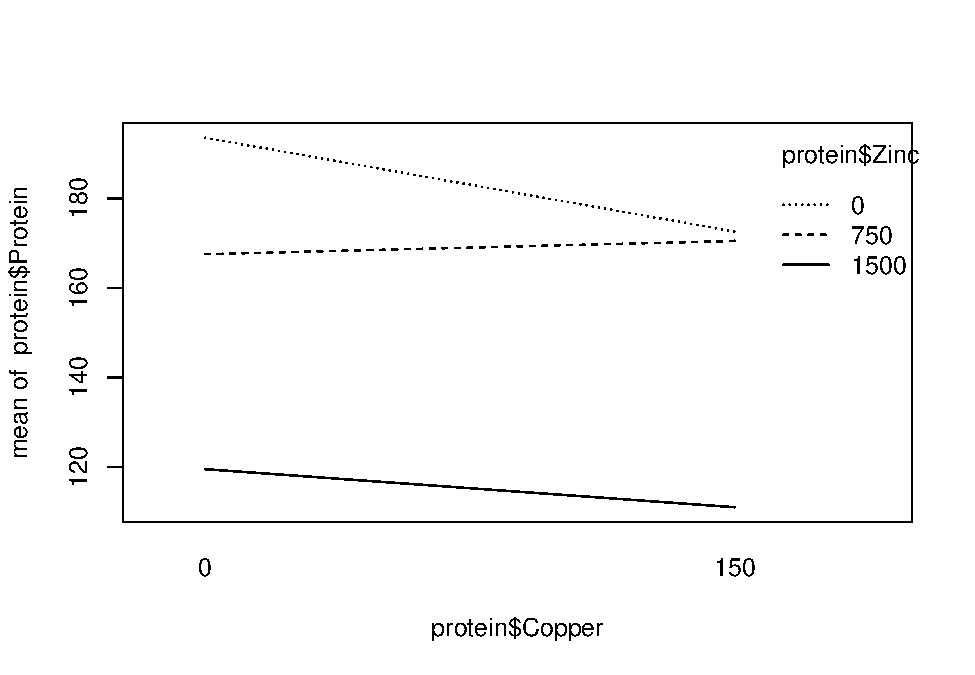
\includegraphics{08-TwoWayANOVA_files/figure-latex/unnamed-chunk-6-1.pdf}

\begin{Shaded}
\begin{Highlighting}[]
\FunctionTok{interaction.plot}\NormalTok{(protein}\SpecialCharTok{$}\NormalTok{Zinc, protein}\SpecialCharTok{$}\NormalTok{Copper, protein}\SpecialCharTok{$}\NormalTok{Protein)}
\end{Highlighting}
\end{Shaded}

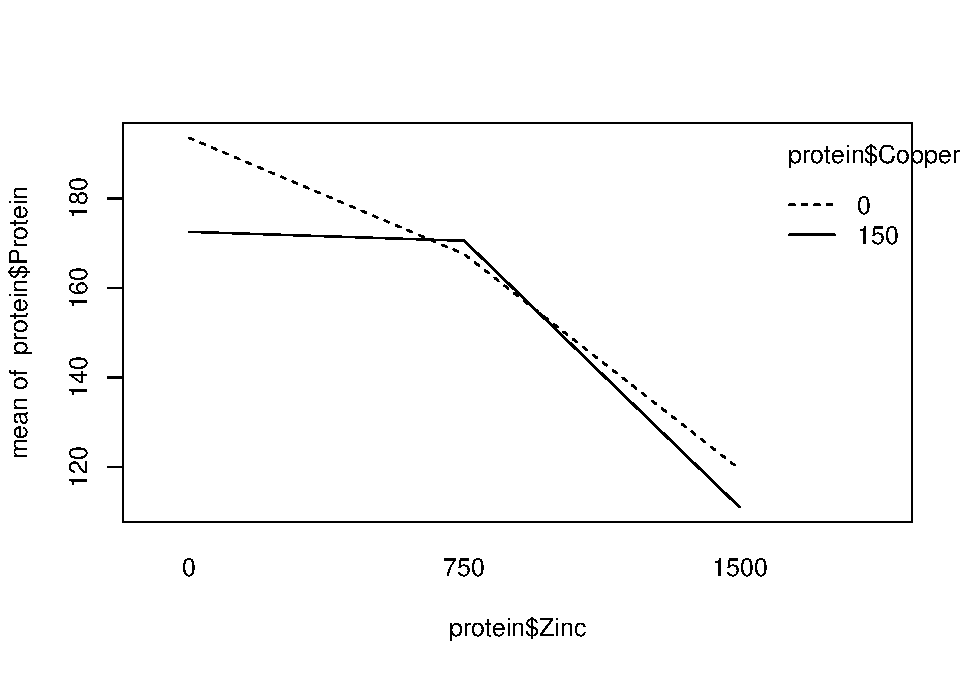
\includegraphics{08-TwoWayANOVA_files/figure-latex/unnamed-chunk-6-2.pdf}

\hypertarget{unbalanced-data-in-two-way-anova}{%
\chapter{Unbalanced data in Two-Way ANOVA}\label{unbalanced-data-in-two-way-anova}}

What happens if \(n_{ij}\) is not the same over crossed levels of the treatment factors? And, worse, what if some combination has zero replicates?!?

This is very common for two reasons: in observational studies researchers have less control over the number of subjects with certain levels of factors. Even when these are controlled through sampling or fixed in experimental studies there will be individuals that are lost/missing for some reason, and this ruins balance.

What goes wrong and what still works? (some of these things we haven't yet defined)
- Comparisons using contrasts - still work!
- Partial F tests in linear model - still work!
- least-squares means - still work!
- Sums of squares (you guessed it) - fails miserably!

Throughout we'll assume missing observations/lack of balance occurs at random, that is, does not have anything to do with treatments. If, however, a treatment level causes loss of observations, our analysis will have problems. You can imagine a treatment that causes side-effects in humans may cause ``loss to follow-up'' when taking before-after measures, because people will dislike the treatment and drop out of the study. So, independence of unbalance and treatment is not always a given.

\hypertarget{raw-and-least-squares-means}{%
\section{Raw and Least-Squares Means}\label{raw-and-least-squares-means}}

Consider a two-way ANOVA where factors A and B each have 2 levels, simplest possible setup. Given observations:

\begin{longtable}[]{@{}llll@{}}
\toprule()
& & Cell Means (Sample Sizes) & \\
\midrule()
\endhead
& & B & \\
& & 1 & 2 \\
A & 1 & 4.90(10) & 2.79(4) \\
& 2 & 8.14(2) & 6.00(4) \\
\bottomrule()
\end{longtable}

When the sample sizes were all equal (balanced) sample means were apples-to-apples. Now, not so much. We can define the ``raw sample means'' (sample-size weighted averages) by \(\overline Y_{1\cdot\cdot} = 4.30= \frac{1}{14}(10\times 4.9 + 4\times 2.79)\). The raw means are misleading if the other factor has an effect, because B at level 1 is more represented in the raw mean average than B at level 2. The difference of raw means \(\overline Y_{1\cdot\cdot} - \overline Y_{2\cdot\cdot}\) also contains an effect from B, which is hidden/disguised when we sum over levels of B. The raw means for factor A are defined \(\mu_{i\cdot}^R = [\sum_{j}n_{ij}]^{-1}\sum_j n_{ij}\mu_{ij}\).

The ``least-squares means'' on the other hand, average the cell means without regard for sample size: mean of level 1 of A is \((2.79+4.9)/2 = 3.85\). The LS means for factor A are defined \(\mu_{i\cdot} = \sum_{j} \mu_{ij}/b\) where \(b\) is the number of levels of B.

When the experiment is balanced, these are equal.

The estimators of the raw means for factor A are simply the raw sample means \(\hat\mu_{i\cdot}^{R} = [\sum_{j}n_{ij}]^{-1}\sum_j n_{ij}\overline Y_{ij}\). These have standard error
\[\text{s.e.}(\hat\mu_{i\cdot}^{R})=\sigma\left[\sum_{j}n_{ij}\right]^{-1/2}.\]
The estimated LS means have standard error
\[\text{s.e.}(\hat\mu_{i\cdot})=\sigma\sqrt{b^{-2}\sum_j n_{ij}^{-1}}.\]

``Simple effects'' compare two levels of one factor at a fixed level of another factor. Differences of LS means are unweighted averages of simple effects:
\[\sum_j(\mu_{ij} - \mu_{i'j})/b\]

\hypertarget{example-turbine-data}{%
\subsection{Example: Turbine data}\label{example-turbine-data}}

The following data describes characteristics of turbine jet engines. Turbine engines feature many spinning blades. Both the position and rate of revolutions of the moving blades affect the behavior of the outflow of air generated by the engines. The Strouhal number is one quantity that characterizes the oscillations of this flow of air. In the following data the Strouhal number is the response variable, and both rate and position of turbine blades are treatment factors.

The turbine data is balanced, but we'll remove a few rows to create imbalance, just for illustration.

\begin{Shaded}
\begin{Highlighting}[]
\NormalTok{strouhal.df }\OtherTok{\textless{}{-}} \FunctionTok{read.csv}\NormalTok{(}\StringTok{\textquotesingle{}flow.csv\textquotesingle{}}\NormalTok{)}
\NormalTok{strouhal.df}
\end{Highlighting}
\end{Shaded}

\begin{verbatim}
##    strouhal position rate
## 1  26016.65       -1    0
## 2  28254.84       -1    0
## 3  27413.45       -1    0
## 4  28556.40       -1    0
## 5  26029.52        1    0
## 6  28270.20        1    0
## 7  27370.98        1    0
## 8  28542.62        1    0
## 9  30359.70       -1    1
## 10 33191.74       -1    1
## 11 31487.19       -1    1
## 12 33111.07       -1    1
## 13 30066.25        1    1
## 14 32868.95        1    1
## 15 31757.56        1    1
## 16 33437.95        1    1
## 17 32189.43       -1    2
## 18 33782.31       -1    2
## 19 34090.11       -1    2
## 20 31098.27       -1    2
## 21 30994.56        1    2
## 22 31013.19        1    2
## 23 34892.13        1    2
## 24 33116.98        1    2
\end{verbatim}

\begin{Shaded}
\begin{Highlighting}[]
\NormalTok{strouhal.df}\OtherTok{\textless{}{-}}\NormalTok{strouhal.df[}\SpecialCharTok{{-}}\FunctionTok{c}\NormalTok{(}\DecValTok{1}\NormalTok{,}\DecValTok{8}\NormalTok{,}\DecValTok{24}\NormalTok{),]}
\NormalTok{strouhal.df}
\end{Highlighting}
\end{Shaded}

\begin{verbatim}
##    strouhal position rate
## 2  28254.84       -1    0
## 3  27413.45       -1    0
## 4  28556.40       -1    0
## 5  26029.52        1    0
## 6  28270.20        1    0
## 7  27370.98        1    0
## 9  30359.70       -1    1
## 10 33191.74       -1    1
## 11 31487.19       -1    1
## 12 33111.07       -1    1
## 13 30066.25        1    1
## 14 32868.95        1    1
## 15 31757.56        1    1
## 16 33437.95        1    1
## 17 32189.43       -1    2
## 18 33782.31       -1    2
## 19 34090.11       -1    2
## 20 31098.27       -1    2
## 21 30994.56        1    2
## 22 31013.19        1    2
## 23 34892.13        1    2
\end{verbatim}

\begin{Shaded}
\begin{Highlighting}[]
\NormalTok{strouhal.df}\SpecialCharTok{$}\NormalTok{position}\OtherTok{\textless{}{-}}\FunctionTok{as.factor}\NormalTok{(strouhal.df}\SpecialCharTok{$}\NormalTok{position)}
\NormalTok{strouhal.df}\SpecialCharTok{$}\NormalTok{rate}\OtherTok{\textless{}{-}}\FunctionTok{as.factor}\NormalTok{(strouhal.df}\SpecialCharTok{$}\NormalTok{rate)}
\end{Highlighting}
\end{Shaded}

Below are the crossed treatment mean responses, the LS means, and the raw means:

\begin{Shaded}
\begin{Highlighting}[]
\FunctionTok{library}\NormalTok{(tidyverse)}
\end{Highlighting}
\end{Shaded}

\begin{verbatim}
## -- Attaching packages --------------------------------------- tidyverse 1.3.2 --
## v ggplot2 3.3.6      v purrr   0.3.4 
## v tibble  3.1.8      v dplyr   1.0.10
## v tidyr   1.2.1      v stringr 1.4.1 
## v readr   2.1.2      v forcats 0.5.2 
## -- Conflicts ------------------------------------------ tidyverse_conflicts() --
## x dplyr::filter() masks stats::filter()
## x dplyr::lag()    masks stats::lag()
\end{verbatim}

\begin{Shaded}
\begin{Highlighting}[]
\NormalTok{by\_trt }\OtherTok{\textless{}{-}} \FunctionTok{group\_by}\NormalTok{(strouhal.df, position, rate)}
\NormalTok{mean\_resp }\OtherTok{\textless{}{-}} \FunctionTok{summarise}\NormalTok{(by\_trt, }\AttributeTok{trt\_mean =} \FunctionTok{mean}\NormalTok{(strouhal))}
\end{Highlighting}
\end{Shaded}

\begin{verbatim}
## `summarise()` has grouped output by 'position'. You can override using the
## `.groups` argument.
\end{verbatim}

\begin{Shaded}
\begin{Highlighting}[]
\NormalTok{mean\_resp}
\end{Highlighting}
\end{Shaded}

\begin{verbatim}
## # A tibble: 6 x 3
## # Groups:   position [2]
##   position rate  trt_mean
##   <fct>    <fct>    <dbl>
## 1 -1       0       28075.
## 2 -1       1       32037.
## 3 -1       2       32790.
## 4 1        0       27224.
## 5 1        1       32033.
## 6 1        2       32300.
\end{verbatim}

\begin{Shaded}
\begin{Highlighting}[]
\NormalTok{mean\_resp}\OtherTok{\textless{}{-}}\FunctionTok{as.matrix}\NormalTok{(mean\_resp[,}\DecValTok{3}\NormalTok{])}
\NormalTok{LS\_mean\_pos }\OtherTok{\textless{}{-}} \FunctionTok{c}\NormalTok{(}\FunctionTok{mean}\NormalTok{(mean\_resp[}\DecValTok{1}\SpecialCharTok{:}\DecValTok{3}\NormalTok{,}\DecValTok{1}\NormalTok{]), }\FunctionTok{mean}\NormalTok{(mean\_resp[}\DecValTok{4}\SpecialCharTok{:}\DecValTok{6}\NormalTok{,}\DecValTok{1}\NormalTok{]))}
\NormalTok{LS\_mean\_pos}
\end{Highlighting}
\end{Shaded}

\begin{verbatim}
## [1] 30967.45 30518.73
\end{verbatim}

\begin{Shaded}
\begin{Highlighting}[]
\NormalTok{LS\_mean\_rate }\OtherTok{\textless{}{-}} \FunctionTok{c}\NormalTok{(}\FunctionTok{mean}\NormalTok{(mean\_resp[}\FunctionTok{c}\NormalTok{(}\DecValTok{1}\NormalTok{,}\DecValTok{4}\NormalTok{),}\DecValTok{1}\NormalTok{]), }\FunctionTok{mean}\NormalTok{(mean\_resp[}\FunctionTok{c}\NormalTok{(}\DecValTok{2}\NormalTok{,}\DecValTok{5}\NormalTok{),}\DecValTok{1}\NormalTok{]), }\FunctionTok{mean}\NormalTok{(mean\_resp[}\FunctionTok{c}\NormalTok{(}\DecValTok{3}\NormalTok{,}\DecValTok{6}\NormalTok{),}\DecValTok{1}\NormalTok{]))}
\NormalTok{LS\_mean\_rate}
\end{Highlighting}
\end{Shaded}

\begin{verbatim}
## [1] 27649.23 32035.05 32544.99
\end{verbatim}

\begin{Shaded}
\begin{Highlighting}[]
\NormalTok{by\_pos }\OtherTok{\textless{}{-}} \FunctionTok{group\_by}\NormalTok{(strouhal.df, position)}
\NormalTok{raw\_mean\_pos }\OtherTok{\textless{}{-}} \FunctionTok{summarise}\NormalTok{(by\_pos, }\AttributeTok{trt\_mean =} \FunctionTok{mean}\NormalTok{(strouhal))}
\NormalTok{raw\_mean\_pos}
\end{Highlighting}
\end{Shaded}

\begin{verbatim}
## # A tibble: 2 x 2
##   position trt_mean
##   <fct>       <dbl>
## 1 -1         31230.
## 2 1          30670.
\end{verbatim}

\begin{Shaded}
\begin{Highlighting}[]
\NormalTok{by\_rate }\OtherTok{\textless{}{-}} \FunctionTok{group\_by}\NormalTok{(strouhal.df, rate)}
\NormalTok{raw\_mean\_rate }\OtherTok{\textless{}{-}} \FunctionTok{summarise}\NormalTok{(by\_rate, }\AttributeTok{trt\_mean =} \FunctionTok{mean}\NormalTok{(strouhal))}
\NormalTok{raw\_mean\_rate}
\end{Highlighting}
\end{Shaded}

\begin{verbatim}
## # A tibble: 3 x 2
##   rate  trt_mean
##   <fct>    <dbl>
## 1 0       27649.
## 2 1       32035.
## 3 2       32580
\end{verbatim}

It is also convenient to compute the LS means using built-in functions from the package emmeans:. The ``emmean'' stands for estimated marginal mean. These are calculated based on a model. If we use the two way model with interaction, then the emmeans are the LS means.

\begin{Shaded}
\begin{Highlighting}[]
\FunctionTok{library}\NormalTok{(emmeans)}
\FunctionTok{emmeans}\NormalTok{(}\FunctionTok{lm}\NormalTok{(strouhal}\SpecialCharTok{\textasciitilde{}}\NormalTok{position}\SpecialCharTok{+}\NormalTok{rate}\SpecialCharTok{+}\NormalTok{position}\SpecialCharTok{*}\NormalTok{rate, }\AttributeTok{data =}\NormalTok{ strouhal.df), }\StringTok{\textquotesingle{}position\textquotesingle{}}\NormalTok{)}
\end{Highlighting}
\end{Shaded}

\begin{verbatim}
## NOTE: Results may be misleading due to involvement in interactions
\end{verbatim}

\begin{verbatim}
##  position emmean  SE df lower.CL upper.CL
##  -1        30967 441 15    30028    31906
##  1         30519 462 15    29534    31504
## 
## Results are averaged over the levels of: rate 
## Confidence level used: 0.95
\end{verbatim}

\begin{Shaded}
\begin{Highlighting}[]
\FunctionTok{emmeans}\NormalTok{(}\FunctionTok{lm}\NormalTok{(strouhal}\SpecialCharTok{\textasciitilde{}}\NormalTok{position}\SpecialCharTok{+}\NormalTok{rate}\SpecialCharTok{+}\NormalTok{position}\SpecialCharTok{*}\NormalTok{rate, }\AttributeTok{data =}\NormalTok{ strouhal.df), }\StringTok{\textquotesingle{}rate\textquotesingle{}}\NormalTok{)}
\end{Highlighting}
\end{Shaded}

\begin{verbatim}
## NOTE: Results may be misleading due to involvement in interactions
\end{verbatim}

\begin{verbatim}
##  rate emmean  SE df lower.CL upper.CL
##  0     27649 591 15    26389    28909
##  1     32035 512 15    30944    33126
##  2     32545 553 15    31367    33723
## 
## Results are averaged over the levels of: position 
## Confidence level used: 0.95
\end{verbatim}

Next, lets compute CIs for contrasts of LS means. For example, consider comparing mean Strouhal values at rate level 0 versus rate level 1. The point estimate is
\[\overline Y_{\cdot,0} - \overline Y_{\cdot,1}\]
the sample LS mean at level zero of rate summed over position minus the sample LS mean at level one of rate summed over position. This difference of sample means has the following standard error:
\begin{align*}
V(\overline Y_{\cdot,0} - \overline Y_{\cdot,1}) & = V(\tfrac12(\overline Y_{-1,0} + \overline Y_{1,0}) -\tfrac12(\overline Y_{-1,1} + \overline Y_{1,1}))//
& = \sigma^2\tfrac14 (1/3 + 1/3 + 1/4 + 1/4)
\end{align*}
using the cell sample sizes calculated in R below.

\begin{Shaded}
\begin{Highlighting}[]
\NormalTok{by\_trt }\OtherTok{\textless{}{-}} \FunctionTok{group\_by}\NormalTok{(strouhal.df, position, rate)}
\NormalTok{n\_resp }\OtherTok{\textless{}{-}} \FunctionTok{summarise}\NormalTok{(by\_trt, }\AttributeTok{trt\_mean =} \FunctionTok{n}\NormalTok{())}
\end{Highlighting}
\end{Shaded}

\begin{verbatim}
## `summarise()` has grouped output by 'position'. You can override using the
## `.groups` argument.
\end{verbatim}

\begin{Shaded}
\begin{Highlighting}[]
\NormalTok{n\_resp}
\end{Highlighting}
\end{Shaded}

\begin{verbatim}
## # A tibble: 6 x 3
## # Groups:   position [2]
##   position rate  trt_mean
##   <fct>    <fct>    <int>
## 1 -1       0            3
## 2 -1       1            4
## 3 -1       2            4
## 4 1        0            3
## 5 1        1            4
## 6 1        2            3
\end{verbatim}

Then, a CI for the difference in LS means is given by
\[\left(\overline Y_{\cdot,0} - \overline Y_{\cdot,1} \pm t_{1-\alpha/2, n-p}\sqrt{MSE\tfrac14 (1/3 + 1/3 + 1/4 + 1/4) }\right)\]

\begin{Shaded}
\begin{Highlighting}[]
\NormalTok{my.lm }\OtherTok{\textless{}{-}} \FunctionTok{summary}\NormalTok{(}\FunctionTok{lm}\NormalTok{(strouhal}\SpecialCharTok{\textasciitilde{}}\NormalTok{position}\SpecialCharTok{+}\NormalTok{rate}\SpecialCharTok{+}\NormalTok{position}\SpecialCharTok{*}\NormalTok{rate, }\AttributeTok{data =}\NormalTok{ strouhal.df))}

\FunctionTok{c}\NormalTok{(LS\_mean\_rate[}\DecValTok{1}\NormalTok{] }\SpecialCharTok{{-}}\NormalTok{ LS\_mean\_rate[}\DecValTok{2}\NormalTok{] }\SpecialCharTok{{-}} \FunctionTok{qt}\NormalTok{(}\FloatTok{0.975}\NormalTok{, my.lm}\SpecialCharTok{$}\NormalTok{df[}\DecValTok{2}\NormalTok{])}\SpecialCharTok{*}\NormalTok{my.lm}\SpecialCharTok{$}\NormalTok{sigma}\SpecialCharTok{*}\FunctionTok{sqrt}\NormalTok{((}\DecValTok{1}\SpecialCharTok{/}\DecValTok{4}\NormalTok{)}\SpecialCharTok{*}\NormalTok{ (}\DecValTok{1}\SpecialCharTok{/}\DecValTok{3} \SpecialCharTok{+} \DecValTok{1}\SpecialCharTok{/}\DecValTok{3} \SpecialCharTok{+} \DecValTok{1}\SpecialCharTok{/}\DecValTok{4} \SpecialCharTok{+} \DecValTok{1}\SpecialCharTok{/}\DecValTok{4}\NormalTok{)), LS\_mean\_rate[}\DecValTok{1}\NormalTok{] }\SpecialCharTok{{-}}\NormalTok{ LS\_mean\_rate[}\DecValTok{2}\NormalTok{] }\SpecialCharTok{+} \FunctionTok{qt}\NormalTok{(}\FloatTok{0.975}\NormalTok{, my.lm}\SpecialCharTok{$}\NormalTok{df[}\DecValTok{2}\NormalTok{])}\SpecialCharTok{*}\NormalTok{my.lm}\SpecialCharTok{$}\NormalTok{sigma}\SpecialCharTok{*}\FunctionTok{sqrt}\NormalTok{((}\DecValTok{1}\SpecialCharTok{/}\DecValTok{4}\NormalTok{)}\SpecialCharTok{*}\NormalTok{ (}\DecValTok{1}\SpecialCharTok{/}\DecValTok{3} \SpecialCharTok{+} \DecValTok{1}\SpecialCharTok{/}\DecValTok{3} \SpecialCharTok{+} \DecValTok{1}\SpecialCharTok{/}\DecValTok{4} \SpecialCharTok{+} \DecValTok{1}\SpecialCharTok{/}\DecValTok{4}\NormalTok{)))}
\end{Highlighting}
\end{Shaded}

\begin{verbatim}
## [1] -6052.374 -2719.265
\end{verbatim}

\hypertarget{partial-f-tests-and-type-iii-ss}{%
\section{Partial F tests and Type III SS}\label{partial-f-tests-and-type-iii-ss}}

To test for interaction and main effects in unbalanced, to-way ANOVA, we cannot use the same sums of squares formulas as before. These do not work for unbalanced data. Essentially, they result in comparisons of raw, rather than LS means.

Instead, we test for interaction and main effects using \emph{partial F tests}. Think of the Gauss-Markov notation \(Y=X\beta+\epsilon\). A partial F test is used to test the hypothesis \(H_0:\text{a certain set of }\beta_j\text{ coefficients is zero}\). The set could be as small as one coefficient, or as large as all the coefficients except for the intercept. Under the null hypothesis, inclusion in the model of the covariates corresponding to these coefficients does not substantially change the predicted responses \(\hat Y\); and, as a result, does not substantially reduce the sum of squared residuals. Therefore, the intuitive test of this null hypothesis is a comparison of SSE under models including versus excluding the given set of covariates:

\[F = \frac{[SSE(\text{reduced model}) - SSE(\text{full model})]/\text{number of excluded coefficients}}{MSE(\text{full model})}\]

Under \(H_0\) the test statistic \(F\) has an \(F\) distribution with numerator degrees of freedom equal to the number of excluded coefficients and denominator degrees of freedom equal to \(n-p\) where the full model coefficient vector \(\beta\) has dimension \(p\times 1\).
SAS, and certain R functions, will report \emph{Type III sums of squares} for unbalanced experiments. These are simply defined by partial F tests. For example, the Type III SS for factor A in a two-way ANOVA with interaction is simply the difference in the sum of squared residuals for the full linear model corresponding to the two-way ANOVA versus the reduced linear model where the columns of \(X\) corresponding to the factor A main effects have been removed. Therefore, tests based on Type III sums of squares are exactly partial F tests.

\hypertarget{example-turbine-data-tests}{%
\subsection{Example: Turbine Data tests}\label{example-turbine-data-tests}}

We can perform partial F tests by fitting reduced and full linear models and comparing sums of squared residuals. The R package \emph{car} will perform these tests automatically using the function \emph{Anova}. The following code computes a tests for the main effect of rate, both ``by hand'' by fitting full and reduced models, and using the Anova function. Note the equivalence of F statistics.

\begin{Shaded}
\begin{Highlighting}[]
\FunctionTok{library}\NormalTok{(car)}
\end{Highlighting}
\end{Shaded}

\begin{verbatim}
## Loading required package: carData
\end{verbatim}

\begin{verbatim}
## 
## Attaching package: 'car'
\end{verbatim}

\begin{verbatim}
## The following object is masked from 'package:dplyr':
## 
##     recode
\end{verbatim}

\begin{verbatim}
## The following object is masked from 'package:purrr':
## 
##     some
\end{verbatim}

\begin{Shaded}
\begin{Highlighting}[]
\FunctionTok{Anova}\NormalTok{(}\FunctionTok{lm}\NormalTok{(strouhal}\SpecialCharTok{\textasciitilde{}}\NormalTok{position }\SpecialCharTok{+}\NormalTok{ rate}\SpecialCharTok{+}\NormalTok{position}\SpecialCharTok{*}\NormalTok{rate, }\AttributeTok{data =}\NormalTok{ strouhal.df), }\AttributeTok{type =} \StringTok{\textquotesingle{}III\textquotesingle{}}\NormalTok{)}
\end{Highlighting}
\end{Shaded}

\begin{verbatim}
## Anova Table (Type III tests)
## 
## Response: strouhal
##                   Sum Sq Df   F value    Pr(>F)    
## (Intercept)   2364599469  1 1128.1201 1.564e-15 ***
## position         1087144  1    0.5187  0.482485    
## rate            42206544  2   10.0681  0.001689 ** 
## position:rate     631584  2    0.1507  0.861425    
## Residuals       31440793 15                        
## ---
## Signif. codes:  0 '***' 0.001 '**' 0.01 '*' 0.05 '.' 0.1 ' ' 1
\end{verbatim}

\begin{Shaded}
\begin{Highlighting}[]
\FunctionTok{summary}\NormalTok{(}\FunctionTok{lm}\NormalTok{(strouhal}\SpecialCharTok{\textasciitilde{}}\NormalTok{position }\SpecialCharTok{+}\NormalTok{ rate}\SpecialCharTok{+}\NormalTok{position}\SpecialCharTok{*}\NormalTok{rate, }\AttributeTok{data =}\NormalTok{ strouhal.df))}
\end{Highlighting}
\end{Shaded}

\begin{verbatim}
## 
## Call:
## lm(formula = strouhal ~ position + rate + position * rate, data = strouhal.df)
## 
## Residuals:
##     Min      1Q  Median      3Q     Max 
## -1966.4 -1194.0   147.4  1046.6  2592.2 
## 
## Coefficients:
##                 Estimate Std. Error t value Pr(>|t|)    
## (Intercept)      28074.9      835.9  33.587 1.56e-15 ***
## position1         -851.3     1182.1  -0.720 0.482485    
## rate1             3962.5     1105.8   3.584 0.002716 ** 
## rate2             4715.1     1105.8   4.264 0.000679 ***
## position1:rate1    846.6     1563.8   0.541 0.596202    
## position1:rate2    361.3     1618.7   0.223 0.826403    
## ---
## Signif. codes:  0 '***' 0.001 '**' 0.01 '*' 0.05 '.' 0.1 ' ' 1
## 
## Residual standard error: 1448 on 15 degrees of freedom
## Multiple R-squared:  0.7511, Adjusted R-squared:  0.6681 
## F-statistic: 9.053 on 5 and 15 DF,  p-value: 0.000396
\end{verbatim}

\begin{Shaded}
\begin{Highlighting}[]
\NormalTok{full.model }\OtherTok{\textless{}{-}} \FunctionTok{lm}\NormalTok{(strouhal}\SpecialCharTok{\textasciitilde{}}\NormalTok{position }\SpecialCharTok{+}\NormalTok{ rate}\SpecialCharTok{+}\NormalTok{position}\SpecialCharTok{*}\NormalTok{rate, }\AttributeTok{data =}\NormalTok{ strouhal.df)}
\NormalTok{SSE.full }\OtherTok{\textless{}{-}} \FunctionTok{sum}\NormalTok{(full.model}\SpecialCharTok{$}\NormalTok{residuals}\SpecialCharTok{\^{}}\DecValTok{2}\NormalTok{)}
\NormalTok{MSE }\OtherTok{\textless{}{-}}\NormalTok{ SSE.full}\SpecialCharTok{/}\NormalTok{(}\FunctionTok{nrow}\NormalTok{(strouhal.df)}\SpecialCharTok{{-}}\DecValTok{6}\NormalTok{)}

\NormalTok{X.R }\OtherTok{\textless{}{-}} \FunctionTok{model.matrix}\NormalTok{(strouhal}\SpecialCharTok{\textasciitilde{}}\NormalTok{position }\SpecialCharTok{+}\NormalTok{ rate}\SpecialCharTok{+}\NormalTok{position}\SpecialCharTok{*}\NormalTok{rate, }\AttributeTok{data =}\NormalTok{ strouhal.df)}
\NormalTok{X.R }\OtherTok{\textless{}{-}}\NormalTok{ X.R[,}\SpecialCharTok{{-}}\FunctionTok{c}\NormalTok{(}\DecValTok{3}\NormalTok{,}\DecValTok{4}\NormalTok{)]}

\NormalTok{beta.hat.R }\OtherTok{\textless{}{-}} \FunctionTok{solve}\NormalTok{(}\FunctionTok{t}\NormalTok{(X.R)}\SpecialCharTok{\%*\%}\NormalTok{X.R)}\SpecialCharTok{\%*\%}\FunctionTok{t}\NormalTok{(X.R)}\SpecialCharTok{\%*\%}\NormalTok{strouhal.df}\SpecialCharTok{$}\NormalTok{strouhal}
\NormalTok{pred.R }\OtherTok{\textless{}{-}}\NormalTok{ X.R}\SpecialCharTok{\%*\%}\NormalTok{beta.hat.R}
\NormalTok{SSE.R }\OtherTok{\textless{}{-}} \FunctionTok{sum}\NormalTok{((strouhal.df}\SpecialCharTok{$}\NormalTok{strouhal }\SpecialCharTok{{-}}\NormalTok{ pred.R)}\SpecialCharTok{\^{}}\DecValTok{2}\NormalTok{)}

\NormalTok{F }\OtherTok{\textless{}{-}}\NormalTok{ ((SSE.R }\SpecialCharTok{{-}}\NormalTok{ SSE.full)}\SpecialCharTok{/}\NormalTok{(}\DecValTok{2}\NormalTok{)) }\SpecialCharTok{/}\NormalTok{ (SSE.full }\SpecialCharTok{/}\NormalTok{ (}\FunctionTok{nrow}\NormalTok{(X.R)}\SpecialCharTok{{-}}\DecValTok{6}\NormalTok{))}
\NormalTok{F}
\end{Highlighting}
\end{Shaded}

\begin{verbatim}
## [1] 10.0681
\end{verbatim}

\hypertarget{follow-up-tests}{%
\section{Follow-up tests}\label{follow-up-tests}}

From the Anova output in the above example we see that the main effect for rate is significant. Since rate has 3 factors, it makes sense to perform Tukey-corrected pairwise comparisons to better understand which levels of rate drive the significance of the effect.

For balanced experiments we typically use the R function TukeyHSD, which takes an aov object as its argument. But, since aov objects are based on Type I SS (raw means) these pairwise comparisons are not the comparisons we want to make. Rather, we want to make pairwise comparisons of LS means.

We can compute these by hand , as we did above for uncorrected pairwise comparisons. The only difference is that we replace the Student's \(t\) quantile in the CI calculation by the upper \(1-\alpha\) quantile of Tukey's Studentized range distribution, multiplied by \(1/\sqrt{2}\).

\hypertarget{example-turbine-data-tukey-corrected-pairwise-comparisons}{%
\subsection{Example: Turbine data Tukey-corrected pairwise comparisons}\label{example-turbine-data-tukey-corrected-pairwise-comparisons}}

\begin{Shaded}
\begin{Highlighting}[]
\NormalTok{n\_resp}
\end{Highlighting}
\end{Shaded}

\begin{verbatim}
## # A tibble: 6 x 3
## # Groups:   position [2]
##   position rate  trt_mean
##   <fct>    <fct>    <int>
## 1 -1       0            3
## 2 -1       1            4
## 3 -1       2            4
## 4 1        0            3
## 5 1        1            4
## 6 1        2            3
\end{verbatim}

\begin{Shaded}
\begin{Highlighting}[]
\FunctionTok{c}\NormalTok{(LS\_mean\_rate[}\DecValTok{1}\NormalTok{] }\SpecialCharTok{{-}}\NormalTok{ LS\_mean\_rate[}\DecValTok{2}\NormalTok{] }\SpecialCharTok{{-}} \FunctionTok{sqrt}\NormalTok{(}\DecValTok{1}\SpecialCharTok{/}\DecValTok{2}\NormalTok{)}\SpecialCharTok{*}\FunctionTok{qtukey}\NormalTok{(}\FloatTok{0.95}\NormalTok{,}\DecValTok{3}\NormalTok{, my.lm}\SpecialCharTok{$}\NormalTok{df[}\DecValTok{2}\NormalTok{])}\SpecialCharTok{*}\NormalTok{my.lm}\SpecialCharTok{$}\NormalTok{sigma}\SpecialCharTok{*}\FunctionTok{sqrt}\NormalTok{((}\DecValTok{1}\SpecialCharTok{/}\DecValTok{4}\NormalTok{)}\SpecialCharTok{*}\NormalTok{ (}\DecValTok{1}\SpecialCharTok{/}\DecValTok{3} \SpecialCharTok{+} \DecValTok{1}\SpecialCharTok{/}\DecValTok{3} \SpecialCharTok{+} \DecValTok{1}\SpecialCharTok{/}\DecValTok{4} \SpecialCharTok{+} \DecValTok{1}\SpecialCharTok{/}\DecValTok{4}\NormalTok{)), LS\_mean\_rate[}\DecValTok{1}\NormalTok{] }\SpecialCharTok{{-}}\NormalTok{ LS\_mean\_rate[}\DecValTok{2}\NormalTok{] }\SpecialCharTok{+} \FunctionTok{sqrt}\NormalTok{(}\DecValTok{1}\SpecialCharTok{/}\DecValTok{2}\NormalTok{)}\SpecialCharTok{*}\FunctionTok{qtukey}\NormalTok{(}\FloatTok{0.95}\NormalTok{,}\DecValTok{3}\NormalTok{, my.lm}\SpecialCharTok{$}\NormalTok{df[}\DecValTok{2}\NormalTok{])}\SpecialCharTok{*}\NormalTok{my.lm}\SpecialCharTok{$}\NormalTok{sigma}\SpecialCharTok{*}\FunctionTok{sqrt}\NormalTok{((}\DecValTok{1}\SpecialCharTok{/}\DecValTok{4}\NormalTok{)}\SpecialCharTok{*}\NormalTok{ (}\DecValTok{1}\SpecialCharTok{/}\DecValTok{3} \SpecialCharTok{+} \DecValTok{1}\SpecialCharTok{/}\DecValTok{3} \SpecialCharTok{+} \DecValTok{1}\SpecialCharTok{/}\DecValTok{4} \SpecialCharTok{+} \DecValTok{1}\SpecialCharTok{/}\DecValTok{4}\NormalTok{)))}
\end{Highlighting}
\end{Shaded}

\begin{verbatim}
## [1] -6416.750 -2354.889
\end{verbatim}

\begin{Shaded}
\begin{Highlighting}[]
\DecValTok{1}\SpecialCharTok{{-}}\FunctionTok{ptukey}\NormalTok{(}\FunctionTok{abs}\NormalTok{(LS\_mean\_rate[}\DecValTok{1}\NormalTok{] }\SpecialCharTok{{-}}\NormalTok{ LS\_mean\_rate[}\DecValTok{2}\NormalTok{])}\SpecialCharTok{/}\NormalTok{(}\FunctionTok{sqrt}\NormalTok{(}\DecValTok{1}\SpecialCharTok{/}\DecValTok{2}\NormalTok{)}\SpecialCharTok{*}\NormalTok{my.lm}\SpecialCharTok{$}\NormalTok{sigma}\SpecialCharTok{*}\FunctionTok{sqrt}\NormalTok{((}\DecValTok{1}\SpecialCharTok{/}\DecValTok{4}\NormalTok{)}\SpecialCharTok{*}\NormalTok{ (}\DecValTok{1}\SpecialCharTok{/}\DecValTok{3} \SpecialCharTok{+} \DecValTok{1}\SpecialCharTok{/}\DecValTok{3} \SpecialCharTok{+} \DecValTok{1}\SpecialCharTok{/}\DecValTok{4} \SpecialCharTok{+} \DecValTok{1}\SpecialCharTok{/}\DecValTok{4}\NormalTok{))), }\DecValTok{3}\NormalTok{, my.lm}\SpecialCharTok{$}\NormalTok{df[}\DecValTok{2}\NormalTok{])}
\end{Highlighting}
\end{Shaded}

\begin{verbatim}
## [1] 0.0001390661
\end{verbatim}

\begin{Shaded}
\begin{Highlighting}[]
\FunctionTok{c}\NormalTok{(LS\_mean\_rate[}\DecValTok{1}\NormalTok{] }\SpecialCharTok{{-}}\NormalTok{ LS\_mean\_rate[}\DecValTok{3}\NormalTok{] }\SpecialCharTok{{-}} \FunctionTok{sqrt}\NormalTok{(}\DecValTok{1}\SpecialCharTok{/}\DecValTok{2}\NormalTok{)}\SpecialCharTok{*}\FunctionTok{qtukey}\NormalTok{(}\FloatTok{0.95}\NormalTok{,}\DecValTok{3}\NormalTok{, my.lm}\SpecialCharTok{$}\NormalTok{df[}\DecValTok{2}\NormalTok{])}\SpecialCharTok{*}\NormalTok{my.lm}\SpecialCharTok{$}\NormalTok{sigma}\SpecialCharTok{*}\FunctionTok{sqrt}\NormalTok{((}\DecValTok{1}\SpecialCharTok{/}\DecValTok{4}\NormalTok{)}\SpecialCharTok{*}\NormalTok{ (}\DecValTok{1}\SpecialCharTok{/}\DecValTok{3} \SpecialCharTok{+} \DecValTok{1}\SpecialCharTok{/}\DecValTok{3} \SpecialCharTok{+} \DecValTok{1}\SpecialCharTok{/}\DecValTok{4} \SpecialCharTok{+} \DecValTok{1}\SpecialCharTok{/}\DecValTok{3}\NormalTok{)), LS\_mean\_rate[}\DecValTok{1}\NormalTok{] }\SpecialCharTok{{-}}\NormalTok{ LS\_mean\_rate[}\DecValTok{2}\NormalTok{] }\SpecialCharTok{+} \FunctionTok{sqrt}\NormalTok{(}\DecValTok{1}\SpecialCharTok{/}\DecValTok{2}\NormalTok{)}\SpecialCharTok{*}\FunctionTok{qtukey}\NormalTok{(}\FloatTok{0.95}\NormalTok{,}\DecValTok{3}\NormalTok{, my.lm}\SpecialCharTok{$}\NormalTok{df[}\DecValTok{2}\NormalTok{])}\SpecialCharTok{*}\NormalTok{my.lm}\SpecialCharTok{$}\NormalTok{sigma}\SpecialCharTok{*}\FunctionTok{sqrt}\NormalTok{((}\DecValTok{1}\SpecialCharTok{/}\DecValTok{4}\NormalTok{)}\SpecialCharTok{*}\NormalTok{ (}\DecValTok{1}\SpecialCharTok{/}\DecValTok{3} \SpecialCharTok{+} \DecValTok{1}\SpecialCharTok{/}\DecValTok{3} \SpecialCharTok{+} \DecValTok{1}\SpecialCharTok{/}\DecValTok{4} \SpecialCharTok{+} \DecValTok{1}\SpecialCharTok{/}\DecValTok{3}\NormalTok{)))}
\end{Highlighting}
\end{Shaded}

\begin{verbatim}
## [1] -6997.976 -2283.607
\end{verbatim}

\begin{Shaded}
\begin{Highlighting}[]
\DecValTok{1}\SpecialCharTok{{-}}\FunctionTok{ptukey}\NormalTok{(}\FunctionTok{abs}\NormalTok{(LS\_mean\_rate[}\DecValTok{1}\NormalTok{] }\SpecialCharTok{{-}}\NormalTok{ LS\_mean\_rate[}\DecValTok{3}\NormalTok{])}\SpecialCharTok{/}\NormalTok{(}\FunctionTok{sqrt}\NormalTok{(}\DecValTok{1}\SpecialCharTok{/}\DecValTok{2}\NormalTok{)}\SpecialCharTok{*}\NormalTok{my.lm}\SpecialCharTok{$}\NormalTok{sigma}\SpecialCharTok{*}\FunctionTok{sqrt}\NormalTok{((}\DecValTok{1}\SpecialCharTok{/}\DecValTok{4}\NormalTok{)}\SpecialCharTok{*}\NormalTok{ (}\DecValTok{1}\SpecialCharTok{/}\DecValTok{3} \SpecialCharTok{+} \DecValTok{1}\SpecialCharTok{/}\DecValTok{3} \SpecialCharTok{+} \DecValTok{1}\SpecialCharTok{/}\DecValTok{4} \SpecialCharTok{+} \DecValTok{1}\SpecialCharTok{/}\DecValTok{3}\NormalTok{))), }\DecValTok{3}\NormalTok{, my.lm}\SpecialCharTok{$}\NormalTok{df[}\DecValTok{2}\NormalTok{])}
\end{Highlighting}
\end{Shaded}

\begin{verbatim}
## [1] 6.250909e-05
\end{verbatim}

\begin{Shaded}
\begin{Highlighting}[]
\FunctionTok{c}\NormalTok{(LS\_mean\_rate[}\DecValTok{2}\NormalTok{] }\SpecialCharTok{{-}}\NormalTok{ LS\_mean\_rate[}\DecValTok{3}\NormalTok{] }\SpecialCharTok{{-}} \FunctionTok{sqrt}\NormalTok{(}\DecValTok{1}\SpecialCharTok{/}\DecValTok{2}\NormalTok{)}\SpecialCharTok{*}\FunctionTok{qtukey}\NormalTok{(}\FloatTok{0.95}\NormalTok{,}\DecValTok{3}\NormalTok{, my.lm}\SpecialCharTok{$}\NormalTok{df[}\DecValTok{2}\NormalTok{])}\SpecialCharTok{*}\NormalTok{my.lm}\SpecialCharTok{$}\NormalTok{sigma}\SpecialCharTok{*}\FunctionTok{sqrt}\NormalTok{((}\DecValTok{1}\SpecialCharTok{/}\DecValTok{4}\NormalTok{)}\SpecialCharTok{*}\NormalTok{ (}\DecValTok{1}\SpecialCharTok{/}\DecValTok{4} \SpecialCharTok{+} \DecValTok{1}\SpecialCharTok{/}\DecValTok{4} \SpecialCharTok{+} \DecValTok{1}\SpecialCharTok{/}\DecValTok{4} \SpecialCharTok{+} \DecValTok{1}\SpecialCharTok{/}\DecValTok{3}\NormalTok{)), LS\_mean\_rate[}\DecValTok{1}\NormalTok{] }\SpecialCharTok{{-}}\NormalTok{ LS\_mean\_rate[}\DecValTok{2}\NormalTok{] }\SpecialCharTok{+} \FunctionTok{sqrt}\NormalTok{(}\DecValTok{1}\SpecialCharTok{/}\DecValTok{2}\NormalTok{)}\SpecialCharTok{*}\FunctionTok{qtukey}\NormalTok{(}\FloatTok{0.95}\NormalTok{,}\DecValTok{3}\NormalTok{, my.lm}\SpecialCharTok{$}\NormalTok{df[}\DecValTok{2}\NormalTok{])}\SpecialCharTok{*}\NormalTok{my.lm}\SpecialCharTok{$}\NormalTok{sigma}\SpecialCharTok{*}\FunctionTok{sqrt}\NormalTok{((}\DecValTok{1}\SpecialCharTok{/}\DecValTok{4}\NormalTok{)}\SpecialCharTok{*}\NormalTok{ (}\DecValTok{1}\SpecialCharTok{/}\DecValTok{4} \SpecialCharTok{+} \DecValTok{1}\SpecialCharTok{/}\DecValTok{4} \SpecialCharTok{+} \DecValTok{1}\SpecialCharTok{/}\DecValTok{4} \SpecialCharTok{+} \DecValTok{1}\SpecialCharTok{/}\DecValTok{3}\NormalTok{)))}
\end{Highlighting}
\end{Shaded}

\begin{verbatim}
## [1] -2466.998 -2428.766
\end{verbatim}

\begin{Shaded}
\begin{Highlighting}[]
\DecValTok{1}\SpecialCharTok{{-}}\FunctionTok{ptukey}\NormalTok{(}\FunctionTok{abs}\NormalTok{(LS\_mean\_rate[}\DecValTok{2}\NormalTok{] }\SpecialCharTok{{-}}\NormalTok{ LS\_mean\_rate[}\DecValTok{3}\NormalTok{])}\SpecialCharTok{/}\NormalTok{(}\FunctionTok{sqrt}\NormalTok{(}\DecValTok{1}\SpecialCharTok{/}\DecValTok{2}\NormalTok{)}\SpecialCharTok{*}\NormalTok{my.lm}\SpecialCharTok{$}\NormalTok{sigma}\SpecialCharTok{*}\FunctionTok{sqrt}\NormalTok{((}\DecValTok{1}\SpecialCharTok{/}\DecValTok{4}\NormalTok{)}\SpecialCharTok{*}\NormalTok{ (}\DecValTok{1}\SpecialCharTok{/}\DecValTok{4} \SpecialCharTok{+} \DecValTok{1}\SpecialCharTok{/}\DecValTok{4} \SpecialCharTok{+} \DecValTok{1}\SpecialCharTok{/}\DecValTok{4} \SpecialCharTok{+} \DecValTok{1}\SpecialCharTok{/}\DecValTok{3}\NormalTok{))), }\DecValTok{3}\NormalTok{, my.lm}\SpecialCharTok{$}\NormalTok{df[}\DecValTok{2}\NormalTok{])}
\end{Highlighting}
\end{Shaded}

\begin{verbatim}
## [1] 0.7802542
\end{verbatim}

\begin{Shaded}
\begin{Highlighting}[]
\FunctionTok{library}\NormalTok{(emmeans)}
\NormalTok{em.strouhal}\OtherTok{\textless{}{-}}\FunctionTok{emmeans}\NormalTok{(}\FunctionTok{lm}\NormalTok{(strouhal}\SpecialCharTok{\textasciitilde{}}\NormalTok{position }\SpecialCharTok{+}\NormalTok{ rate}\SpecialCharTok{+}\NormalTok{position}\SpecialCharTok{*}\NormalTok{rate, }\AttributeTok{data =}\NormalTok{ strouhal.df), }\StringTok{"rate"}\NormalTok{)}
\end{Highlighting}
\end{Shaded}

\begin{verbatim}
## NOTE: Results may be misleading due to involvement in interactions
\end{verbatim}

\begin{Shaded}
\begin{Highlighting}[]
\FunctionTok{pairs}\NormalTok{(em.strouhal, }\AttributeTok{adjust =} \StringTok{\textquotesingle{}tukey\textquotesingle{}}\NormalTok{)}
\end{Highlighting}
\end{Shaded}

\begin{verbatim}
##  contrast      estimate  SE df t.ratio p.value
##  rate0 - rate1    -4386 782 15  -5.609  0.0001
##  rate0 - rate2    -4896 809 15  -6.049  0.0001
##  rate1 - rate2     -510 753 15  -0.677  0.7803
## 
## Results are averaged over the levels of: position 
## P value adjustment: tukey method for comparing a family of 3 estimates
\end{verbatim}

\hypertarget{unbalanced-data-and-simpsons-paradox}{%
\section{Unbalanced data and Simpson's Paradox}\label{unbalanced-data-and-simpsons-paradox}}

The following toy example of unbalanced data helps illustrate the difference between using raw and LS means. The LS mean response for A level 1 is larger (-0.3) than the LS mean response for A level 2 (-0.7). And, the mean response when A is level 1 is larger than when A is level 2 for every level of B. However, for raw means, the reverse is true (-1.975 vs.~0.225)! If we look at the data we see this is due to the fact more samples are observed for the levels of B when A is level 1 and the response is lowest (10) compared to when it is highest (5). Basically, the sampling is biased towards levels of B where the A level 1 response is low and the A level 2 response is high. The raw means are not capturing a real difference in effect of A; rather, they are capturing a difference in sample weighting.

This is an example of \textbf{Simpson's Paradox} where the direction of an effect may change if effects are weighted by sample size.

\begin{Shaded}
\begin{Highlighting}[]
\NormalTok{Y1 }\OtherTok{\textless{}{-}}\NormalTok{ (}\DecValTok{1}\SpecialCharTok{:}\DecValTok{5}\NormalTok{)}\SpecialCharTok{+}\FloatTok{0.1}
\NormalTok{Y2 }\OtherTok{\textless{}{-}}\NormalTok{ (}\DecValTok{1}\SpecialCharTok{:}\DecValTok{5}\NormalTok{)}
\NormalTok{Y3 }\OtherTok{\textless{}{-}} \FunctionTok{c}\NormalTok{((}\DecValTok{1}\SpecialCharTok{:}\DecValTok{5}\NormalTok{)}\SpecialCharTok{{-}}\DecValTok{10}\NormalTok{,(}\DecValTok{1}\SpecialCharTok{:}\DecValTok{5}\NormalTok{)}\SpecialCharTok{{-}}\DecValTok{10}\NormalTok{) }
\NormalTok{Y4 }\OtherTok{\textless{}{-}} \FunctionTok{c}\NormalTok{((}\DecValTok{1}\SpecialCharTok{:}\DecValTok{5}\NormalTok{),}\DecValTok{1}\SpecialCharTok{:}\DecValTok{5}\NormalTok{)}
\NormalTok{Y5 }\OtherTok{\textless{}{-}}\NormalTok{ (}\DecValTok{1}\SpecialCharTok{:}\DecValTok{5}\NormalTok{)}\SpecialCharTok{{-}}\FloatTok{0.1}
\NormalTok{Y6 }\OtherTok{\textless{}{-}}\NormalTok{ (}\DecValTok{1}\SpecialCharTok{:}\DecValTok{5}\NormalTok{)}\SpecialCharTok{{-}}\DecValTok{11}

\NormalTok{A }\OtherTok{\textless{}{-}} \FunctionTok{c}\NormalTok{(}\FunctionTok{rep}\NormalTok{(}\DecValTok{1}\NormalTok{,}\DecValTok{20}\NormalTok{),}\FunctionTok{rep}\NormalTok{(}\DecValTok{2}\NormalTok{,}\DecValTok{20}\NormalTok{))}
\NormalTok{B }\OtherTok{\textless{}{-}} \FunctionTok{c}\NormalTok{(}\FunctionTok{rep}\NormalTok{(}\DecValTok{1}\NormalTok{,}\DecValTok{5}\NormalTok{),}\FunctionTok{rep}\NormalTok{(}\DecValTok{2}\NormalTok{,}\DecValTok{5}\NormalTok{), }\FunctionTok{rep}\NormalTok{(}\DecValTok{3}\NormalTok{,}\DecValTok{10}\NormalTok{),}\FunctionTok{rep}\NormalTok{(}\DecValTok{1}\NormalTok{,}\DecValTok{10}\NormalTok{),}\FunctionTok{rep}\NormalTok{(}\DecValTok{2}\NormalTok{,}\DecValTok{5}\NormalTok{), }\FunctionTok{rep}\NormalTok{(}\DecValTok{3}\NormalTok{,}\DecValTok{5}\NormalTok{))}
\NormalTok{Y }\OtherTok{\textless{}{-}} \FunctionTok{c}\NormalTok{(Y1,Y2,Y3,Y4,Y5,Y6)}
\NormalTok{data.df }\OtherTok{\textless{}{-}} \FunctionTok{data.frame}\NormalTok{(}\AttributeTok{Y=}\NormalTok{Y,}\AttributeTok{A=}\FunctionTok{as.factor}\NormalTok{(A),}\AttributeTok{B=}\FunctionTok{as.factor}\NormalTok{(B))}

\NormalTok{by\_trt }\OtherTok{\textless{}{-}} \FunctionTok{group\_by}\NormalTok{(data.df, A,B)}
\FunctionTok{summarise}\NormalTok{(by\_trt, }\AttributeTok{trt\_mean =} \FunctionTok{mean}\NormalTok{(Y))}
\end{Highlighting}
\end{Shaded}

\begin{verbatim}
## `summarise()` has grouped output by 'A'. You can override using the `.groups`
## argument.
\end{verbatim}

\begin{verbatim}
## # A tibble: 6 x 3
## # Groups:   A [2]
##   A     B     trt_mean
##   <fct> <fct>    <dbl>
## 1 1     1          3.1
## 2 1     2          3  
## 3 1     3         -7  
## 4 2     1          3  
## 5 2     2          2.9
## 6 2     3         -8
\end{verbatim}

\begin{Shaded}
\begin{Highlighting}[]
\FunctionTok{emmeans}\NormalTok{(}\FunctionTok{lm}\NormalTok{(Y}\SpecialCharTok{\textasciitilde{}}\NormalTok{A}\SpecialCharTok{+}\NormalTok{B}\SpecialCharTok{+}\NormalTok{A}\SpecialCharTok{*}\NormalTok{B, }\AttributeTok{data =}\NormalTok{ data.df), }\StringTok{"A"}\NormalTok{)}
\end{Highlighting}
\end{Shaded}

\begin{verbatim}
## NOTE: Results may be misleading due to involvement in interactions
\end{verbatim}

\begin{verbatim}
##  A emmean    SE df lower.CL upper.CL
##  1   -0.3 0.362 34    -1.03   0.4348
##  2   -0.7 0.362 34    -1.43   0.0348
## 
## Results are averaged over the levels of: B 
## Confidence level used: 0.95
\end{verbatim}

\begin{Shaded}
\begin{Highlighting}[]
\FunctionTok{emmeans}\NormalTok{(}\FunctionTok{lm}\NormalTok{(Y}\SpecialCharTok{\textasciitilde{}}\NormalTok{A}\SpecialCharTok{+}\NormalTok{B}\SpecialCharTok{+}\NormalTok{A}\SpecialCharTok{*}\NormalTok{B, }\AttributeTok{data =}\NormalTok{ data.df), }\StringTok{"B"}\NormalTok{)}
\end{Highlighting}
\end{Shaded}

\begin{verbatim}
## NOTE: Results may be misleading due to involvement in interactions
\end{verbatim}

\begin{verbatim}
##  B emmean    SE df lower.CL upper.CL
##  1   3.05 0.420 34     2.20     3.90
##  2   2.95 0.485 34     1.96     3.94
##  3  -7.50 0.420 34    -8.35    -6.65
## 
## Results are averaged over the levels of: A 
## Confidence level used: 0.95
\end{verbatim}

\begin{Shaded}
\begin{Highlighting}[]
\FunctionTok{mean}\NormalTok{(data.df}\SpecialCharTok{$}\NormalTok{Y[data.df}\SpecialCharTok{$}\NormalTok{A}\SpecialCharTok{==}\DecValTok{1}\NormalTok{])}
\end{Highlighting}
\end{Shaded}

\begin{verbatim}
## [1] -1.975
\end{verbatim}

\begin{Shaded}
\begin{Highlighting}[]
\FunctionTok{mean}\NormalTok{(data.df}\SpecialCharTok{$}\NormalTok{Y[data.df}\SpecialCharTok{$}\NormalTok{A}\SpecialCharTok{==}\DecValTok{2}\NormalTok{])}
\end{Highlighting}
\end{Shaded}

\begin{verbatim}
## [1] 0.225
\end{verbatim}

\begin{Shaded}
\begin{Highlighting}[]
\FunctionTok{mean}\NormalTok{(data.df}\SpecialCharTok{$}\NormalTok{Y[data.df}\SpecialCharTok{$}\NormalTok{B}\SpecialCharTok{==}\DecValTok{1}\NormalTok{])}
\end{Highlighting}
\end{Shaded}

\begin{verbatim}
## [1] 3.033333
\end{verbatim}

\begin{Shaded}
\begin{Highlighting}[]
\FunctionTok{mean}\NormalTok{(data.df}\SpecialCharTok{$}\NormalTok{Y[data.df}\SpecialCharTok{$}\NormalTok{B}\SpecialCharTok{==}\DecValTok{2}\NormalTok{])}
\end{Highlighting}
\end{Shaded}

\begin{verbatim}
## [1] 2.95
\end{verbatim}

\begin{Shaded}
\begin{Highlighting}[]
\FunctionTok{mean}\NormalTok{(data.df}\SpecialCharTok{$}\NormalTok{Y[data.df}\SpecialCharTok{$}\NormalTok{B}\SpecialCharTok{==}\DecValTok{3}\NormalTok{])}
\end{Highlighting}
\end{Shaded}

\begin{verbatim}
## [1] -7.333333
\end{verbatim}

\hypertarget{missing-cells-in-two-way-anova}{%
\chapter{Missing Cells in Two-Way ANOVA}\label{missing-cells-in-two-way-anova}}

In this section we consider how to analyze a two-factor experiment when one crossed treatment is unobserved. If there is no interaction, then this is not problem. But, when interaction is present the lack of observations in a crossed treatment group makes it challenging to assess those interactions. There are, essentially, two ways to proceed: 1) use a one-way model, treating the observed crossed treatments as the levels; or, 2) do a partial two-way analysis.

Below, we illustrate these two approaches in the context of a horticulture experiment about jalapenos.

\hypertarget{anova-with-missing-at-random-cell}{%
\section{ANOVA with missing ``at random'' cell}\label{anova-with-missing-at-random-cell}}

Scoville (spiciness) measure of jalapeno peppers grown under 3 different watering regimens and 3 different levels of sun exposure.

Unbalanced treatment groups with a missing crossed treatment, sun level 3 with water level 3.

\begin{Shaded}
\begin{Highlighting}[]
\NormalTok{my.data}
\end{Highlighting}
\end{Shaded}

\begin{verbatim}
##    scoville water.lvl sun.lvl
## 1       259         1       1
## 2       271         1       1
## 3       289         2       1
## 4       255         2       1
## 5       361         2       1
## 6       118         2       1
## 7       463         3       1
## 8       372         3       1
## 9       372         3       1
## 10      208         1       2
## 11      288         1       2
## 12      482         1       2
## 13      337         1       2
## 14      452         2       2
## 15      325         2       2
## 16      582         3       2
## 17      411         3       2
## 18      467         3       2
## 19      512         1       3
## 20      430         1       3
## 21      478         1       3
## 22      646         2       3
## 23      436         2       3
## 24      345         2       3
\end{verbatim}

\begin{Shaded}
\begin{Highlighting}[]
\FunctionTok{kable}\NormalTok{(}\FunctionTok{aggregate}\NormalTok{(scoville}\SpecialCharTok{\textasciitilde{}}\NormalTok{water.lvl}\SpecialCharTok{+}\NormalTok{sun.lvl}\SpecialCharTok{+}\NormalTok{water.lvl}\SpecialCharTok{*}\NormalTok{sun.lvl, }\AttributeTok{data =}\NormalTok{ my.data, }\AttributeTok{FUN=}\NormalTok{mean))}
\end{Highlighting}
\end{Shaded}

\begin{tabular}{l|l|r}
\hline
water.lvl & sun.lvl & scoville\\
\hline
1 & 1 & 265.0000\\
\hline
2 & 1 & 255.7500\\
\hline
3 & 1 & 402.3333\\
\hline
1 & 2 & 328.7500\\
\hline
2 & 2 & 388.5000\\
\hline
3 & 2 & 486.6667\\
\hline
1 & 3 & 473.3333\\
\hline
2 & 3 & 475.6667\\
\hline
\end{tabular}

\begin{Shaded}
\begin{Highlighting}[]
\FunctionTok{interaction.plot}\NormalTok{(water.lvl, sun.lvl,  scoville, }\AttributeTok{data =}\NormalTok{ my.data)}
\end{Highlighting}
\end{Shaded}

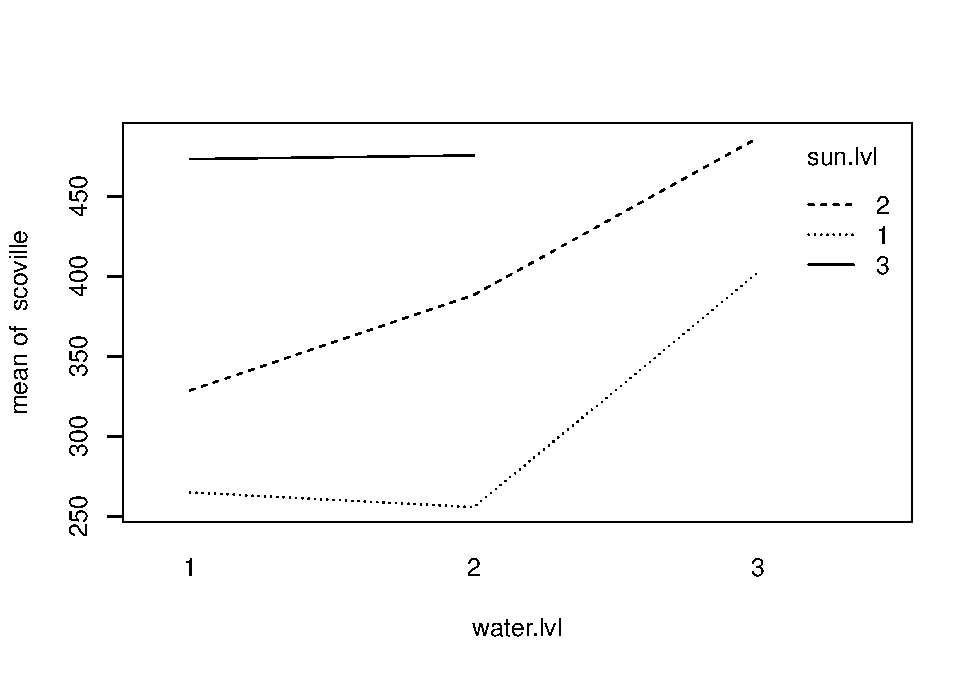
\includegraphics{10-MissingCellsInTwoWay_files/figure-latex/unnamed-chunk-3-1.pdf}

\begin{Shaded}
\begin{Highlighting}[]
\FunctionTok{boxplot}\NormalTok{(scoville}\SpecialCharTok{\textasciitilde{}}\NormalTok{water.lvl}\SpecialCharTok{+}\NormalTok{ sun.lvl, }\AttributeTok{data =}\NormalTok{ my.data)}
\end{Highlighting}
\end{Shaded}

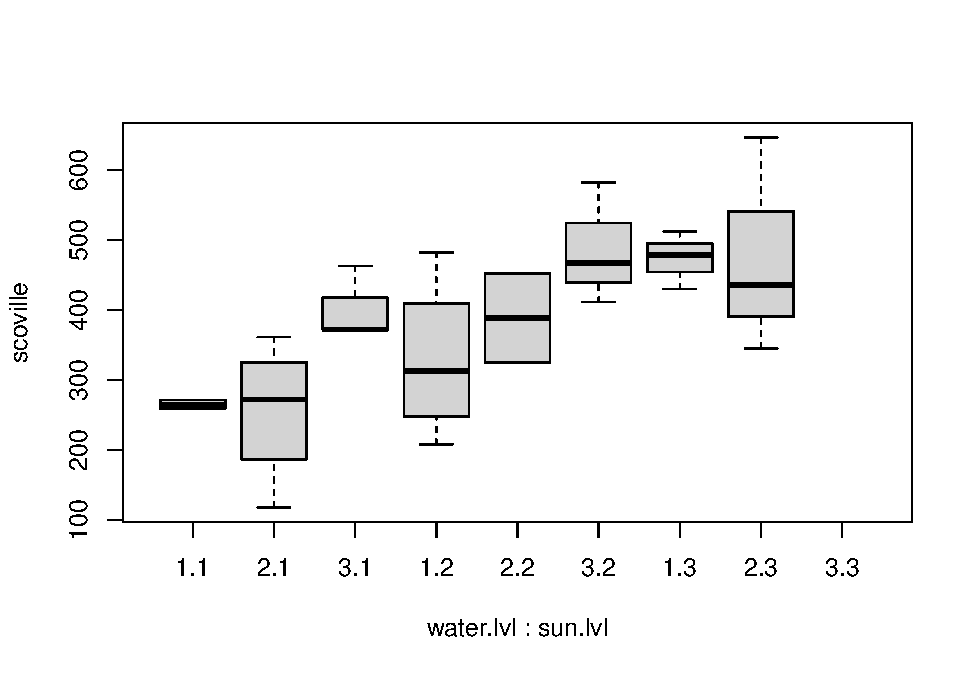
\includegraphics{10-MissingCellsInTwoWay_files/figure-latex/unnamed-chunk-3-2.pdf}

\hypertarget{do-any-of-the-treatments-matter}{%
\section{Do any of the treatments matter?}\label{do-any-of-the-treatments-matter}}

Can test this two equivalent ways:
1. fit a one way anova (ignoring that there are two treatment variables) and test if the treatments are different.
2. fit a linear model and perform the model F test comparing the full model to the intercept only model.

The linear model method is slightly more challenging to implement because of the additional constraint imposed by the missing cell. We have to modify the design matrix from the model.matrix function, or define it by hand.

One way anova below. Notice it says the treatments are not all the same; their mean responses significantly differ for at least one treatment compared to the other 7. One approach would be to follow this test up with tests of contrasts or pairwise comparisons, corrected using Scheff\textquotesingle e or Tukey. Since the data is unbalanced, we should do these by hand.\\
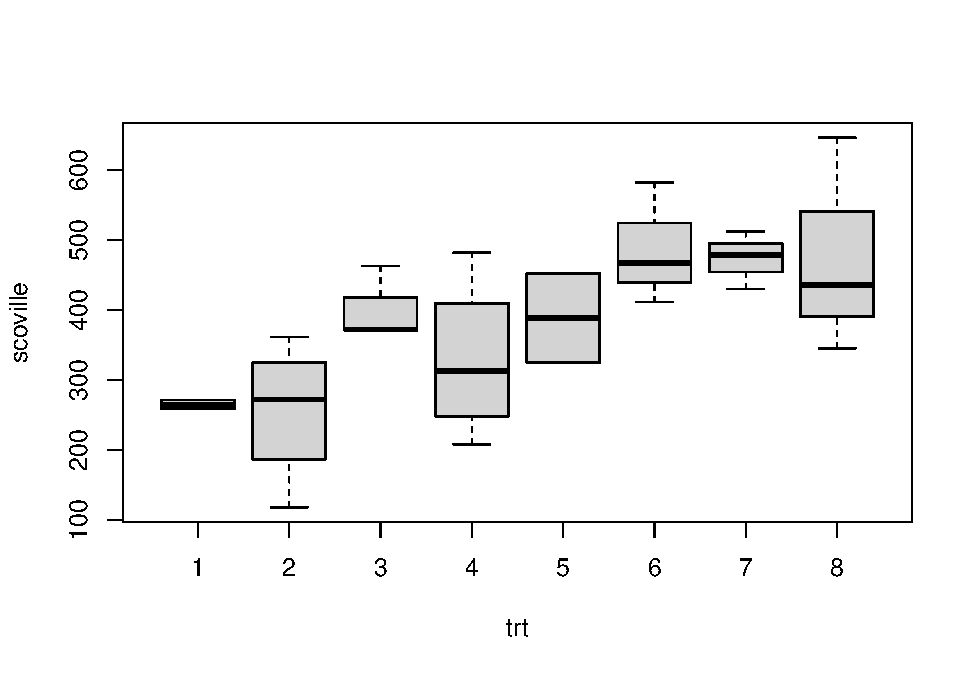
\includegraphics{10-MissingCellsInTwoWay_files/figure-latex/unnamed-chunk-4-1.pdf}

\begin{Shaded}
\begin{Highlighting}[]
\NormalTok{my.data.oneway}
\end{Highlighting}
\end{Shaded}

\begin{verbatim}
##    scoville trt
## 1       259   1
## 2       271   1
## 3       289   2
## 4       255   2
## 5       361   2
## 6       118   2
## 7       463   3
## 8       372   3
## 9       372   3
## 10      208   4
## 11      288   4
## 12      482   4
## 13      337   4
## 14      452   5
## 15      325   5
## 16      582   6
## 17      411   6
## 18      467   6
## 19      512   7
## 20      430   7
## 21      478   7
## 22      646   8
## 23      436   8
## 24      345   8
\end{verbatim}

\begin{Shaded}
\begin{Highlighting}[]
\FunctionTok{library}\NormalTok{(car)}
\FunctionTok{Anova}\NormalTok{(}\FunctionTok{lm}\NormalTok{(scoville}\SpecialCharTok{\textasciitilde{}}\NormalTok{trt, }\AttributeTok{data =}\NormalTok{ my.data.oneway), }\AttributeTok{type =} \StringTok{\textquotesingle{}III\textquotesingle{}}\NormalTok{)}
\end{Highlighting}
\end{Shaded}

\begin{verbatim}
## Anova Table (Type III tests)
## 
## Response: scoville
##              Sum Sq Df  F value   Pr(>F)    
## (Intercept) 3339450  1 354.1618 2.44e-12 ***
## trt          188009  7   2.8484   0.0393 *  
## Residuals    150867 16                      
## ---
## Signif. codes:  0 '***' 0.001 '**' 0.01 '*' 0.05 '.' 0.1 ' ' 1
\end{verbatim}

\hypertarget{fit-a-linear-model-with-additional-constraints}{%
\section{Fit a linear model with additional constraints}\label{fit-a-linear-model-with-additional-constraints}}

The other option for testing if any treatments matter is to fit a linear model. However, we cannot estimate all the parameters of the effects model due to missing the combination of sun level 3 and water level 3. We can only estimate 8 parameters: intercept, 2 for sun, 2 for water, and 3 (rather than 4) interactions. The way to deal with this is to find the full model matrix and then omit the last column corresponding to the interaction that is not estimable. IF we just use the lm() function, we'll get an error, but it will still give us some useful output. Again, we end up having to do some things by hand.

\begin{Shaded}
\begin{Highlighting}[]
\FunctionTok{options}\NormalTok{(}\AttributeTok{contrasts =} \FunctionTok{c}\NormalTok{(}\StringTok{\textquotesingle{}contr.sum\textquotesingle{}}\NormalTok{, }\StringTok{\textquotesingle{}contr.sum\textquotesingle{}}\NormalTok{))}
\NormalTok{my.lm}\OtherTok{\textless{}{-}}\FunctionTok{lm}\NormalTok{(scoville}\SpecialCharTok{\textasciitilde{}}\NormalTok{water.lvl}\SpecialCharTok{+}\NormalTok{sun.lvl}\SpecialCharTok{+}\NormalTok{water.lvl}\SpecialCharTok{*}\NormalTok{sun.lvl, }\AttributeTok{data =}\NormalTok{ my.data)}
\FunctionTok{summary}\NormalTok{(my.lm)}
\end{Highlighting}
\end{Shaded}

\begin{verbatim}
## 
## Call:
## lm(formula = scoville ~ water.lvl + sun.lvl + water.lvl * sun.lvl, 
##     data = my.data)
## 
## Residuals:
##      Min       1Q   Median       3Q      Max 
## -137.750  -41.396   -3.375   44.167  170.333 
## 
## Coefficients: (1 not defined because of singularities)
##                     Estimate Std. Error t value Pr(>|t|)    
## (Intercept)           386.11      41.79   9.240 8.15e-08 ***
## water.lvl1            -30.42      48.55  -0.626    0.540    
## water.lvl2            -12.81      52.02  -0.246    0.809    
## sun.lvl1              -78.42      48.55  -1.615    0.126    
## sun.lvl2               15.19      52.02   0.292    0.774    
## water.lvl1:sun.lvl1   -12.28      49.44  -0.248    0.807    
## water.lvl2:sun.lvl1   -39.14      68.02  -0.575    0.573    
## water.lvl1:sun.lvl2   -42.14      68.02  -0.619    0.544    
## water.lvl2:sun.lvl2       NA         NA      NA       NA    
## ---
## Signif. codes:  0 '***' 0.001 '**' 0.01 '*' 0.05 '.' 0.1 ' ' 1
## 
## Residual standard error: 97.1 on 16 degrees of freedom
## Multiple R-squared:  0.5548, Adjusted R-squared:   0.36 
## F-statistic: 2.848 on 7 and 16 DF,  p-value: 0.0393
\end{verbatim}

\begin{Shaded}
\begin{Highlighting}[]
\NormalTok{my.lm}\SpecialCharTok{$}\NormalTok{coefficients}
\end{Highlighting}
\end{Shaded}

\begin{verbatim}
##         (Intercept)          water.lvl1          water.lvl2            sun.lvl1 
##           386.11111           -30.41667           -12.80556           -78.41667 
##            sun.lvl2 water.lvl1:sun.lvl1 water.lvl2:sun.lvl1 water.lvl1:sun.lvl2 
##            15.19444           -12.27778           -39.13889           -42.13889 
## water.lvl2:sun.lvl2 
##                  NA
\end{verbatim}

\begin{Shaded}
\begin{Highlighting}[]
\NormalTok{X }\OtherTok{\textless{}{-}} \FunctionTok{model.matrix}\NormalTok{(scoville}\SpecialCharTok{\textasciitilde{}}\NormalTok{water.lvl}\SpecialCharTok{+}\NormalTok{sun.lvl}\SpecialCharTok{+}\NormalTok{water.lvl}\SpecialCharTok{*}\NormalTok{sun.lvl, }\AttributeTok{data =}\NormalTok{ my.data)}
\NormalTok{X}
\end{Highlighting}
\end{Shaded}

\begin{verbatim}
##    (Intercept) water.lvl1 water.lvl2 sun.lvl1 sun.lvl2 water.lvl1:sun.lvl1
## 1            1          1          0        1        0                   1
## 2            1          1          0        1        0                   1
## 3            1          0          1        1        0                   0
## 4            1          0          1        1        0                   0
## 5            1          0          1        1        0                   0
## 6            1          0          1        1        0                   0
## 7            1         -1         -1        1        0                  -1
## 8            1         -1         -1        1        0                  -1
## 9            1         -1         -1        1        0                  -1
## 10           1          1          0        0        1                   0
## 11           1          1          0        0        1                   0
## 12           1          1          0        0        1                   0
## 13           1          1          0        0        1                   0
## 14           1          0          1        0        1                   0
## 15           1          0          1        0        1                   0
## 16           1         -1         -1        0        1                   0
## 17           1         -1         -1        0        1                   0
## 18           1         -1         -1        0        1                   0
## 19           1          1          0       -1       -1                  -1
## 20           1          1          0       -1       -1                  -1
## 21           1          1          0       -1       -1                  -1
## 22           1          0          1       -1       -1                   0
## 23           1          0          1       -1       -1                   0
## 24           1          0          1       -1       -1                   0
##    water.lvl2:sun.lvl1 water.lvl1:sun.lvl2 water.lvl2:sun.lvl2
## 1                    0                   0                   0
## 2                    0                   0                   0
## 3                    1                   0                   0
## 4                    1                   0                   0
## 5                    1                   0                   0
## 6                    1                   0                   0
## 7                   -1                   0                   0
## 8                   -1                   0                   0
## 9                   -1                   0                   0
## 10                   0                   1                   0
## 11                   0                   1                   0
## 12                   0                   1                   0
## 13                   0                   1                   0
## 14                   0                   0                   1
## 15                   0                   0                   1
## 16                   0                  -1                  -1
## 17                   0                  -1                  -1
## 18                   0                  -1                  -1
## 19                   0                  -1                   0
## 20                   0                  -1                   0
## 21                   0                  -1                   0
## 22                  -1                   0                  -1
## 23                  -1                   0                  -1
## 24                  -1                   0                  -1
## attr(,"assign")
## [1] 0 1 1 2 2 3 3 3 3
## attr(,"contrasts")
## attr(,"contrasts")$water.lvl
## [1] "contr.sum"
## 
## attr(,"contrasts")$sun.lvl
## [1] "contr.sum"
\end{verbatim}

\begin{Shaded}
\begin{Highlighting}[]
\NormalTok{X }\OtherTok{\textless{}{-}}\NormalTok{ X[,}\SpecialCharTok{{-}}\DecValTok{9}\NormalTok{]}
\NormalTok{beta.hat }\OtherTok{\textless{}{-}} \FunctionTok{solve}\NormalTok{(}\FunctionTok{t}\NormalTok{(X)}\SpecialCharTok{\%*\%}\NormalTok{X)}\SpecialCharTok{\%*\%}\FunctionTok{t}\NormalTok{(X)}\SpecialCharTok{\%*\%}\NormalTok{my.data}\SpecialCharTok{$}\NormalTok{scoville}
\NormalTok{beta.hat}
\end{Highlighting}
\end{Shaded}

\begin{verbatim}
##                          [,1]
## (Intercept)         386.11111
## water.lvl1          -30.41667
## water.lvl2          -12.80556
## sun.lvl1            -78.41667
## sun.lvl2             15.19444
## water.lvl1:sun.lvl1 -12.27778
## water.lvl2:sun.lvl1 -39.13889
## water.lvl1:sun.lvl2 -42.13889
\end{verbatim}

\begin{Shaded}
\begin{Highlighting}[]
\NormalTok{Y.pred }\OtherTok{\textless{}{-}}\NormalTok{X}\SpecialCharTok{\%*\%}\NormalTok{beta.hat}
\NormalTok{SSE }\OtherTok{\textless{}{-}} \FunctionTok{sum}\NormalTok{((my.data}\SpecialCharTok{$}\NormalTok{scoville}\SpecialCharTok{{-}}\NormalTok{Y.pred)}\SpecialCharTok{\^{}}\DecValTok{2}\NormalTok{)}
\NormalTok{MSE }\OtherTok{\textless{}{-}}\NormalTok{ SSE }\SpecialCharTok{/}\NormalTok{ (}\DecValTok{24} \SpecialCharTok{{-}} \DecValTok{8}\NormalTok{)}
\NormalTok{MSE}
\end{Highlighting}
\end{Shaded}

\begin{verbatim}
## [1] 9429.167
\end{verbatim}

\hypertarget{general-linear-test-for-interaction}{%
\section{General Linear Test for interaction}\label{general-linear-test-for-interaction}}

The linear model we just developed, with the additional constraint, allows us to perform more tests. We can use this model to perform General linear F tests for interaction and main effects.

The first estimated interaction parameter
\[1/3 * [\mu_{11} - \mu_{13} - (\mu_{31}-\mu_{32}) - (\mu_{22} - \mu_{23})]\]
(265.0000 - 473.3333 - (402.3333 - 486.6667) - (388.5000 - 475.6667))/3
= -12.27778

The test for interaction does not reject the null hypothesis of no interaction.
Note, we cannot feed the Anova function the fitted linear model; it will produce an error because of the inability to fit all 9 parameters. So, we had to do this ``by hand''.

\begin{Shaded}
\begin{Highlighting}[]
\FunctionTok{options}\NormalTok{(}\AttributeTok{contrasts =} \FunctionTok{c}\NormalTok{(}\StringTok{\textquotesingle{}contr.sum\textquotesingle{}}\NormalTok{, }\StringTok{\textquotesingle{}contr.sum\textquotesingle{}}\NormalTok{))}
\FunctionTok{aggregate}\NormalTok{(scoville}\SpecialCharTok{\textasciitilde{}}\NormalTok{water.lvl}\SpecialCharTok{+}\NormalTok{sun.lvl}\SpecialCharTok{+}\NormalTok{water.lvl}\SpecialCharTok{*}\NormalTok{sun.lvl, }\AttributeTok{data =}\NormalTok{ my.data, }\AttributeTok{FUN=}\NormalTok{mean)}
\end{Highlighting}
\end{Shaded}

\begin{verbatim}
##   water.lvl sun.lvl scoville
## 1         1       1 265.0000
## 2         2       1 255.7500
## 3         3       1 402.3333
## 4         1       2 328.7500
## 5         2       2 388.5000
## 6         3       2 486.6667
## 7         1       3 473.3333
## 8         2       3 475.6667
\end{verbatim}

\begin{Shaded}
\begin{Highlighting}[]
\NormalTok{X }\OtherTok{\textless{}{-}} \FunctionTok{model.matrix}\NormalTok{(scoville}\SpecialCharTok{\textasciitilde{}}\NormalTok{water.lvl}\SpecialCharTok{+}\NormalTok{sun.lvl}\SpecialCharTok{+}\NormalTok{water.lvl}\SpecialCharTok{*}\NormalTok{sun.lvl, }\AttributeTok{data =}\NormalTok{ my.data)}
\NormalTok{X.R }\OtherTok{\textless{}{-}}\NormalTok{ X[,}\DecValTok{1}\SpecialCharTok{:}\DecValTok{5}\NormalTok{]  }\CommentTok{\# no interaction parameters}
\NormalTok{beta.hat.R }\OtherTok{\textless{}{-}} \FunctionTok{solve}\NormalTok{(}\FunctionTok{t}\NormalTok{(X.R)}\SpecialCharTok{\%*\%}\NormalTok{X.R)}\SpecialCharTok{\%*\%}\FunctionTok{t}\NormalTok{(X.R)}\SpecialCharTok{\%*\%}\NormalTok{my.data}\SpecialCharTok{$}\NormalTok{scoville}
\NormalTok{beta.hat.R}
\end{Highlighting}
\end{Shaded}

\begin{verbatim}
##                   [,1]
## (Intercept)  407.58333
## water.lvl1   -54.98160
## water.lvl2   -38.85173
## sun.lvl1    -102.70887
## sun.lvl2     -11.12446
\end{verbatim}

\begin{Shaded}
\begin{Highlighting}[]
\NormalTok{Y.pred.R }\OtherTok{\textless{}{-}}\NormalTok{X.R}\SpecialCharTok{\%*\%}\NormalTok{beta.hat.R}
\NormalTok{SSE.R }\OtherTok{\textless{}{-}} \FunctionTok{sum}\NormalTok{((my.data}\SpecialCharTok{$}\NormalTok{scoville}\SpecialCharTok{{-}}\NormalTok{Y.pred.R)}\SpecialCharTok{\^{}}\DecValTok{2}\NormalTok{)}
\NormalTok{F }\OtherTok{\textless{}{-}}\NormalTok{ ((SSE.R }\SpecialCharTok{{-}}\NormalTok{ SSE)}\SpecialCharTok{/}\NormalTok{(}\DecValTok{3}\NormalTok{)) }\SpecialCharTok{/}\NormalTok{ MSE}
\DecValTok{1}\SpecialCharTok{{-}}\FunctionTok{pf}\NormalTok{(F,}\DecValTok{3}\NormalTok{,}\DecValTok{16}\NormalTok{)}
\end{Highlighting}
\end{Shaded}

\begin{verbatim}
## [1] 0.9381543
\end{verbatim}

\begin{Shaded}
\begin{Highlighting}[]
\CommentTok{\#library(car)}
\CommentTok{\#Anova(lm(scoville\textasciitilde{}water.lvl+sun.lvl+water.lvl*sun.lvl, data = my.data), type = \textquotesingle{}III\textquotesingle{})}
\end{Highlighting}
\end{Shaded}

\hypertarget{partial-analysis-for-interaction}{%
\section{Partial analysis for interaction}\label{partial-analysis-for-interaction}}

An alternative approach is to break the ANOVA into ``overlapping'' pieces that have no missing cells.\\
Break down the table into two overlapping pieces, one with no sun level 3 and one with no water level 3. Let's work with the no sun level 3 table. The idea is the same for the other table. We can test for interaction and main effects within this table. Now, there are 6 treatments, so we estimate an intercept, two water parameters, 1 sun parameter, and 2 interaction parameters.
The first interaction term (no sun level 3 table) is estimating
\[\frac{1}{3}(\mu_{11} -\mu_{12}) -  \frac{1}{6}(\mu_{21}- \mu_{22}) - \frac{1}{6}(\mu_{31} - \mu_{32})\]
\[265/3 - 255.7500/6 - 402.3333/6-328.7500/3+388.500/6+486.6667/6=14.93057\]
Compare this interaction term to the linear model with the additional constraint. I think it seems like a more interpretable interaction term, which I believe is why some people like the partial analysis.

\begin{Shaded}
\begin{Highlighting}[]
\FunctionTok{options}\NormalTok{(}\AttributeTok{contrasts =} \FunctionTok{c}\NormalTok{(}\StringTok{\textquotesingle{}contr.sum\textquotesingle{}}\NormalTok{, }\StringTok{\textquotesingle{}contr.sum\textquotesingle{}}\NormalTok{))}
\FunctionTok{set.seed}\NormalTok{(}\DecValTok{12345}\NormalTok{)}
\NormalTok{water.lvl }\OtherTok{\textless{}{-}} \FunctionTok{as.factor}\NormalTok{(}\DecValTok{1}\SpecialCharTok{+}\FunctionTok{c}\NormalTok{(}\DecValTok{0}\NormalTok{,}\DecValTok{0}\NormalTok{,}\DecValTok{1}\NormalTok{,}\DecValTok{1}\NormalTok{,}\DecValTok{1}\NormalTok{,}\DecValTok{1}\NormalTok{,}\DecValTok{2}\NormalTok{,}\DecValTok{2}\NormalTok{,}\DecValTok{2}\NormalTok{,}\DecValTok{0}\NormalTok{,}\DecValTok{0}\NormalTok{,}\DecValTok{0}\NormalTok{,}\DecValTok{0}\NormalTok{,}\DecValTok{1}\NormalTok{,}\DecValTok{1}\NormalTok{,}\DecValTok{2}\NormalTok{,}\DecValTok{2}\NormalTok{,}\DecValTok{2}\NormalTok{))}
\NormalTok{sun.lvl }\OtherTok{\textless{}{-}} \FunctionTok{as.factor}\NormalTok{(  }\DecValTok{1}\SpecialCharTok{+}\FunctionTok{c}\NormalTok{(}\DecValTok{0}\NormalTok{,}\DecValTok{0}\NormalTok{,}\DecValTok{0}\NormalTok{,}\DecValTok{0}\NormalTok{,}\DecValTok{0}\NormalTok{,}\DecValTok{0}\NormalTok{,}\DecValTok{0}\NormalTok{,}\DecValTok{0}\NormalTok{,}\DecValTok{0}\NormalTok{,}\DecValTok{1}\NormalTok{,}\DecValTok{1}\NormalTok{,}\DecValTok{1}\NormalTok{,}\DecValTok{1}\NormalTok{,}\DecValTok{1}\NormalTok{,}\DecValTok{1}\NormalTok{,}\DecValTok{1}\NormalTok{,}\DecValTok{1}\NormalTok{,}\DecValTok{1}\NormalTok{))}
\NormalTok{scoville }\OtherTok{\textless{}{-}} \FunctionTok{round}\NormalTok{(}\FunctionTok{rnorm}\NormalTok{(}\DecValTok{18}\NormalTok{, }\DecValTok{100}\SpecialCharTok{*}\NormalTok{(}\FunctionTok{as.numeric}\NormalTok{(water.lvl)}\SpecialCharTok{+}\FunctionTok{as.numeric}\NormalTok{(sun.lvl)),}\DecValTok{100}\NormalTok{),}\DecValTok{0}\NormalTok{)}
\NormalTok{my.data1 }\OtherTok{\textless{}{-}} \FunctionTok{data.frame}\NormalTok{(scoville, water.lvl, sun.lvl)}

\FunctionTok{aggregate}\NormalTok{(scoville}\SpecialCharTok{\textasciitilde{}}\NormalTok{water.lvl}\SpecialCharTok{+}\NormalTok{sun.lvl}\SpecialCharTok{+}\NormalTok{water.lvl}\SpecialCharTok{*}\NormalTok{sun.lvl, }\AttributeTok{data =}\NormalTok{ my.data1, }\AttributeTok{FUN=}\NormalTok{mean)}
\end{Highlighting}
\end{Shaded}

\begin{verbatim}
##   water.lvl sun.lvl scoville
## 1         1       1 265.0000
## 2         2       1 255.7500
## 3         3       1 402.3333
## 4         1       2 328.7500
## 5         2       2 388.5000
## 6         3       2 486.6667
\end{verbatim}

\begin{Shaded}
\begin{Highlighting}[]
\FunctionTok{library}\NormalTok{(car)}
\FunctionTok{Anova}\NormalTok{(}\FunctionTok{lm}\NormalTok{(scoville}\SpecialCharTok{\textasciitilde{}}\NormalTok{water.lvl}\SpecialCharTok{+}\NormalTok{sun.lvl}\SpecialCharTok{+}\NormalTok{water.lvl}\SpecialCharTok{*}\NormalTok{sun.lvl, }\AttributeTok{data =}\NormalTok{ my.data1),}\AttributeTok{type =} \StringTok{\textquotesingle{}III\textquotesingle{}}\NormalTok{)}
\end{Highlighting}
\end{Shaded}

\begin{verbatim}
## Anova Table (Type III tests)
## 
## Response: scoville
##                    Sum Sq Df  F value    Pr(>F)    
## (Intercept)       2088060  1 251.0408 2.075e-09 ***
## water.lvl           71684  2   4.3092   0.03887 *  
## sun.lvl             36400  1   4.3763   0.05837 .  
## water.lvl:sun.lvl    3360  2   0.2020   0.81984    
## Residuals           99811 12                       
## ---
## Signif. codes:  0 '***' 0.001 '**' 0.01 '*' 0.05 '.' 0.1 ' ' 1
\end{verbatim}

\begin{Shaded}
\begin{Highlighting}[]
\FunctionTok{summary}\NormalTok{(}\FunctionTok{lm}\NormalTok{(scoville}\SpecialCharTok{\textasciitilde{}}\NormalTok{water.lvl}\SpecialCharTok{+}\NormalTok{sun.lvl}\SpecialCharTok{+}\NormalTok{water.lvl}\SpecialCharTok{*}\NormalTok{sun.lvl, }\AttributeTok{data =}\NormalTok{ my.data1))}
\end{Highlighting}
\end{Shaded}

\begin{verbatim}
## 
## Call:
## lm(formula = scoville ~ water.lvl + sun.lvl + water.lvl * sun.lvl, 
##     data = my.data1)
## 
## Residuals:
##      Min       1Q   Median       3Q      Max 
## -137.750  -38.146   -3.375   53.812  153.250 
## 
## Coefficients:
##                     Estimate Std. Error t value Pr(>|t|)    
## (Intercept)           354.50      22.37  15.844 2.07e-09 ***
## water.lvl1            -57.62      31.94  -1.804   0.0964 .  
## water.lvl2            -32.38      31.94  -1.013   0.3308    
## sun.lvl1              -46.81      22.37  -2.092   0.0584 .  
## water.lvl1:sun.lvl1    14.93      31.94   0.467   0.6486    
## water.lvl2:sun.lvl1   -19.57      31.94  -0.613   0.5516    
## ---
## Signif. codes:  0 '***' 0.001 '**' 0.01 '*' 0.05 '.' 0.1 ' ' 1
## 
## Residual standard error: 91.2 on 12 degrees of freedom
## Multiple R-squared:  0.5438, Adjusted R-squared:  0.3538 
## F-statistic: 2.861 on 5 and 12 DF,  p-value: 0.06299
\end{verbatim}

\begin{Shaded}
\begin{Highlighting}[]
\NormalTok{X }\OtherTok{\textless{}{-}} \FunctionTok{model.matrix}\NormalTok{(scoville}\SpecialCharTok{\textasciitilde{}}\NormalTok{water.lvl}\SpecialCharTok{+}\NormalTok{sun.lvl}\SpecialCharTok{+}\NormalTok{water.lvl}\SpecialCharTok{*}\NormalTok{sun.lvl, }\AttributeTok{data =}\NormalTok{ my.data1)}
\NormalTok{X}
\end{Highlighting}
\end{Shaded}

\begin{verbatim}
##    (Intercept) water.lvl1 water.lvl2 sun.lvl1 water.lvl1:sun.lvl1
## 1            1          1          0        1                   1
## 2            1          1          0        1                   1
## 3            1          0          1        1                   0
## 4            1          0          1        1                   0
## 5            1          0          1        1                   0
## 6            1          0          1        1                   0
## 7            1         -1         -1        1                  -1
## 8            1         -1         -1        1                  -1
## 9            1         -1         -1        1                  -1
## 10           1          1          0       -1                  -1
## 11           1          1          0       -1                  -1
## 12           1          1          0       -1                  -1
## 13           1          1          0       -1                  -1
## 14           1          0          1       -1                   0
## 15           1          0          1       -1                   0
## 16           1         -1         -1       -1                   1
## 17           1         -1         -1       -1                   1
## 18           1         -1         -1       -1                   1
##    water.lvl2:sun.lvl1
## 1                    0
## 2                    0
## 3                    1
## 4                    1
## 5                    1
## 6                    1
## 7                   -1
## 8                   -1
## 9                   -1
## 10                   0
## 11                   0
## 12                   0
## 13                   0
## 14                  -1
## 15                  -1
## 16                   1
## 17                   1
## 18                   1
## attr(,"assign")
## [1] 0 1 1 2 3 3
## attr(,"contrasts")
## attr(,"contrasts")$water.lvl
## [1] "contr.sum"
## 
## attr(,"contrasts")$sun.lvl
## [1] "contr.sum"
\end{verbatim}

\begin{Shaded}
\begin{Highlighting}[]
\FunctionTok{solve}\NormalTok{(}\FunctionTok{t}\NormalTok{(X)}\SpecialCharTok{\%*\%}\NormalTok{X)}\SpecialCharTok{\%*\%}\FunctionTok{t}\NormalTok{(X)}\SpecialCharTok{\%*\%}\NormalTok{my.data1}\SpecialCharTok{$}\NormalTok{scoville}
\end{Highlighting}
\end{Shaded}

\begin{verbatim}
##                          [,1]
## (Intercept)         354.50000
## water.lvl1          -57.62500
## water.lvl2          -32.37500
## sun.lvl1            -46.80556
## water.lvl1:sun.lvl1  14.93056
## water.lvl2:sun.lvl1 -19.56944
\end{verbatim}

\hypertarget{tests-for-main-effects-in-the-partial-table}{%
\section{Tests for main effects in the partial table}\label{tests-for-main-effects-in-the-partial-table}}

(no sun level 3)
We can match the main effects tests in the ANOVA (type 3) table by comparing LS means.

\begin{Shaded}
\begin{Highlighting}[]
\CommentTok{\# contrast test for sun}
\FunctionTok{aggregate}\NormalTok{(scoville}\SpecialCharTok{\textasciitilde{}}\NormalTok{water.lvl}\SpecialCharTok{+}\NormalTok{sun.lvl}\SpecialCharTok{+}\NormalTok{water.lvl}\SpecialCharTok{*}\NormalTok{sun.lvl, }\AttributeTok{data =}\NormalTok{ my.data1, }\AttributeTok{FUN=}\NormalTok{mean)}
\end{Highlighting}
\end{Shaded}

\begin{verbatim}
##   water.lvl sun.lvl scoville
## 1         1       1 265.0000
## 2         2       1 255.7500
## 3         3       1 402.3333
## 4         1       2 328.7500
## 5         2       2 388.5000
## 6         3       2 486.6667
\end{verbatim}

\begin{Shaded}
\begin{Highlighting}[]
\NormalTok{MSE }\OtherTok{\textless{}{-}} \FunctionTok{sum}\NormalTok{(}\FunctionTok{lm}\NormalTok{(scoville}\SpecialCharTok{\textasciitilde{}}\NormalTok{water.lvl}\SpecialCharTok{+}\NormalTok{sun.lvl}\SpecialCharTok{+}\NormalTok{water.lvl}\SpecialCharTok{*}\NormalTok{sun.lvl, }\AttributeTok{data =}\NormalTok{ my.data1)}\SpecialCharTok{$}\NormalTok{residuals}\SpecialCharTok{\^{}}\DecValTok{2}\NormalTok{)}\SpecialCharTok{/}\NormalTok{(}\DecValTok{18{-}6}\NormalTok{)}
\NormalTok{MSE}
\end{Highlighting}
\end{Shaded}

\begin{verbatim}
## [1] 8317.611
\end{verbatim}

\begin{Shaded}
\begin{Highlighting}[]
\NormalTok{(((}\DecValTok{265}\FloatTok{+255.75+402.333}\NormalTok{)}\SpecialCharTok{/}\DecValTok{3}\NormalTok{)}\SpecialCharTok{{-}}\NormalTok{((}\FloatTok{328.75+388.5+486.667}\NormalTok{)}\SpecialCharTok{/}\DecValTok{3}\NormalTok{))}\SpecialCharTok{/}\FunctionTok{sqrt}\NormalTok{(MSE }\SpecialCharTok{*} \DecValTok{2}\SpecialCharTok{*}\NormalTok{(}\DecValTok{1}\SpecialCharTok{/}\DecValTok{9} \SpecialCharTok{*}\NormalTok{ (}\DecValTok{1}\SpecialCharTok{/}\DecValTok{2}\SpecialCharTok{+}\DecValTok{1}\SpecialCharTok{/}\DecValTok{4}\SpecialCharTok{+}\DecValTok{1}\SpecialCharTok{/}\DecValTok{3}\NormalTok{)))}
\end{Highlighting}
\end{Shaded}

\begin{verbatim}
## [1] -2.091965
\end{verbatim}

\begin{Shaded}
\begin{Highlighting}[]
\NormalTok{F}\OtherTok{\textless{}{-}}\NormalTok{((((}\DecValTok{265}\FloatTok{+255.75+402.333}\NormalTok{)}\SpecialCharTok{/}\DecValTok{3}\NormalTok{)}\SpecialCharTok{{-}}\NormalTok{((}\FloatTok{328.75+388.5+486.667}\NormalTok{)}\SpecialCharTok{/}\DecValTok{3}\NormalTok{))}\SpecialCharTok{/}\FunctionTok{sqrt}\NormalTok{(MSE }\SpecialCharTok{*} \DecValTok{2}\SpecialCharTok{*}\NormalTok{(}\DecValTok{1}\SpecialCharTok{/}\DecValTok{9} \SpecialCharTok{*}\NormalTok{ (}\DecValTok{1}\SpecialCharTok{/}\DecValTok{2}\SpecialCharTok{+}\DecValTok{1}\SpecialCharTok{/}\DecValTok{4}\SpecialCharTok{+}\DecValTok{1}\SpecialCharTok{/}\DecValTok{3}\NormalTok{)))}
\NormalTok{)}\SpecialCharTok{\^{}}\DecValTok{2}
\NormalTok{F}
\end{Highlighting}
\end{Shaded}

\begin{verbatim}
## [1] 4.376316
\end{verbatim}

\begin{Shaded}
\begin{Highlighting}[]
\DecValTok{1}\SpecialCharTok{{-}}\FunctionTok{pf}\NormalTok{(F,}\DecValTok{1}\NormalTok{,}\DecValTok{12}\NormalTok{)}
\end{Highlighting}
\end{Shaded}

\begin{verbatim}
## [1] 0.05837152
\end{verbatim}

These tests for main effects should be constructed using the MSE from the full linear model fitted above rather than the partial tables. There is not much of a difference in the conclusion, but the partial table seems to underestimate the variance because it excludes sun level 3 which has larger responses.

\begin{Shaded}
\begin{Highlighting}[]
\CommentTok{\# contrast test for sun}
\FunctionTok{aggregate}\NormalTok{(scoville}\SpecialCharTok{\textasciitilde{}}\NormalTok{water.lvl}\SpecialCharTok{+}\NormalTok{sun.lvl}\SpecialCharTok{+}\NormalTok{water.lvl}\SpecialCharTok{*}\NormalTok{sun.lvl, }\AttributeTok{data =}\NormalTok{ my.data1, }\AttributeTok{FUN=}\NormalTok{mean)}
\end{Highlighting}
\end{Shaded}

\begin{verbatim}
##   water.lvl sun.lvl scoville
## 1         1       1 265.0000
## 2         2       1 255.7500
## 3         3       1 402.3333
## 4         1       2 328.7500
## 5         2       2 388.5000
## 6         3       2 486.6667
\end{verbatim}

\begin{Shaded}
\begin{Highlighting}[]
\NormalTok{MSE }\OtherTok{\textless{}{-}} \FunctionTok{sum}\NormalTok{(}\FunctionTok{lm}\NormalTok{(scoville}\SpecialCharTok{\textasciitilde{}}\NormalTok{water.lvl}\SpecialCharTok{+}\NormalTok{sun.lvl}\SpecialCharTok{+}\NormalTok{water.lvl}\SpecialCharTok{*}\NormalTok{sun.lvl, }\AttributeTok{data =}\NormalTok{ my.data)}\SpecialCharTok{$}\NormalTok{residuals}\SpecialCharTok{\^{}}\DecValTok{2}\NormalTok{)}\SpecialCharTok{/}\NormalTok{(}\DecValTok{24{-}8}\NormalTok{)}
\NormalTok{MSE}
\end{Highlighting}
\end{Shaded}

\begin{verbatim}
## [1] 9429.167
\end{verbatim}

\begin{Shaded}
\begin{Highlighting}[]
\NormalTok{(((}\DecValTok{265}\FloatTok{+255.75+402.333}\NormalTok{)}\SpecialCharTok{/}\DecValTok{3}\NormalTok{)}\SpecialCharTok{{-}}\NormalTok{((}\FloatTok{328.75+388.5+486.667}\NormalTok{)}\SpecialCharTok{/}\DecValTok{3}\NormalTok{))}\SpecialCharTok{/}\FunctionTok{sqrt}\NormalTok{(MSE }\SpecialCharTok{*} \DecValTok{2}\SpecialCharTok{*}\NormalTok{(}\DecValTok{1}\SpecialCharTok{/}\DecValTok{9} \SpecialCharTok{*}\NormalTok{ (}\DecValTok{1}\SpecialCharTok{/}\DecValTok{2}\SpecialCharTok{+}\DecValTok{1}\SpecialCharTok{/}\DecValTok{4}\SpecialCharTok{+}\DecValTok{1}\SpecialCharTok{/}\DecValTok{3}\NormalTok{)))}
\end{Highlighting}
\end{Shaded}

\begin{verbatim}
## [1] -1.964794
\end{verbatim}

\begin{Shaded}
\begin{Highlighting}[]
\NormalTok{F }\OtherTok{\textless{}{-}}\NormalTok{ ((((}\DecValTok{265}\FloatTok{+255.75+402.333}\NormalTok{)}\SpecialCharTok{/}\DecValTok{3}\NormalTok{)}\SpecialCharTok{{-}}\NormalTok{((}\FloatTok{328.75+388.5+486.667}\NormalTok{)}\SpecialCharTok{/}\DecValTok{3}\NormalTok{))}\SpecialCharTok{/}\FunctionTok{sqrt}\NormalTok{(MSE }\SpecialCharTok{*} \DecValTok{2}\SpecialCharTok{*}\NormalTok{(}\DecValTok{1}\SpecialCharTok{/}\DecValTok{9} \SpecialCharTok{*}\NormalTok{ (}\DecValTok{1}\SpecialCharTok{/}\DecValTok{2}\SpecialCharTok{+}\DecValTok{1}\SpecialCharTok{/}\DecValTok{4}\SpecialCharTok{+}\DecValTok{1}\SpecialCharTok{/}\DecValTok{3}\NormalTok{)))}
\NormalTok{)}\SpecialCharTok{\^{}}\DecValTok{2}
\NormalTok{F}
\end{Highlighting}
\end{Shaded}

\begin{verbatim}
## [1] 3.860415
\end{verbatim}

\begin{Shaded}
\begin{Highlighting}[]
\DecValTok{1}\SpecialCharTok{{-}}\FunctionTok{pf}\NormalTok{(F,}\DecValTok{1}\NormalTok{,}\DecValTok{16}\NormalTok{)}
\end{Highlighting}
\end{Shaded}

\begin{verbatim}
## [1] 0.06704815
\end{verbatim}

\hypertarget{strategy-for-analysis-in-two-factor-models}{%
\chapter{Strategy for Analysis in Two-Factor models}\label{strategy-for-analysis-in-two-factor-models}}

In this section we synthesize the main points from our discussion of two-way ANOVA to outline a general strategy for analyzing data from two-factor experiments.

For experiments in which it is known that factors do not interact, comparisons for treatments are made on the basis of factor-level means \(\mu_{i\cdot}\) and \(\mu_{\cdot j}\):
1. Fit the additive model
\[Y_{ijk} = \mu+\alpha_i +\tau_j + \epsilon_{jik},\]
and test for significance of the model using a partial F test comparing the intercept-only model to the full model. If the hypothesis \(H_0:\text{only the intercept is nonzero}\) is rejected, then move to step 2.
2. Test for significance of Factor A main effects, \(H_0:\alpha_i = 0, \text{ for all }i\) versus \(H_a:\text{not all }\alpha_i = 0\).
3. If we reject \(H_0\), move to 4. Otherwise, perform follow-up comparisons of the factor level means \(\mu_{i\cdot}\). These comparisons may be pairwise, or more general contrasts, but should be corrected by Tukey's or Scheff\textquotesingle e's technique.
4. Test for significance of Factor B main effects, \(H_0:\tau_j = 0, \text{ for all }j\) versus \(H_a:\text{not all }\tau_j = 0\). And, again, if we reject \(H_0\), then perform corrected follow-up comparisons of \(\mu_{\cdot j}\)'s.
The above tests for main effects may be conducted using Type 1 sums of squares for balanced experiments, and Type 3 sums of squares (equivalently partial F tests) for unbalanced experiments. For experiments with one or more missing cells, fit a linear model (with extra constraint(s)) and test the main effects using partial F tests.

When interactions may be present, the analysis is more complicated.
1. Fit the model with interactions
\[Y_{ijk} = \mu+\alpha_i +\tau_j + (\alpha\tau)_{ij} + \epsilon_{jik},\]
and test for significance of the model using a partial F test comparing the intercept-only model to the full model. If the hypothesis \(H_0:\text{only the intercept is nonzero}\) is rejected, then move to step 2.
2. Test for significance of the interaction terms \(H_0:(\alpha\tau)_{ij} = 0 \text{ for all }i,j\) versus \(H_a:\text{not all }(\alpha\tau)_{ij}=0\).
3. If we reject \(H_0\), then perform any desired follow-up tests (CIs) for pairwise comparisons or contrasts of the crossed factor treatment means, the \(\mu_{ij}\)'s. For multiple such comparisons use Tukey or Scheff\textquotesingle e adjustments.
4. If we fail to reject the null hypothesis of no interaction, then carry out the tests for main effects. The test for Factor A main effects has null and alternative hypotheses \(H_0:\alpha_i = 0 \text{ for all }i\) versus \(H_a:\text{not all }\alpha_i = 0\). Likewise, the test for Factor B main effects has hypotheses \(H_0:\tau_j = 0, \text{ for all }j\) versus \(H_a:\text{not all }\tau_j = 0\).
5. For each test of main effects, if we reject the null hypothesis, then we may consider conducting follow-up tests to compare the factor-level mean responses, the \(\mu_{i\cdot}\)'s and/or \(\mu_{\cdot j}\)'s. For multiple such comparisons, again, use Tukey or Scheff\textquotesingle e corrections.

Remarks:
1. For the model fit with interaction terms, should we fail to reject the null hypothesis of no interaction, it is generally not appropriate to refit the model without interaction terms. Consider the following reasoning. We used some degrees of freedom (we used data) to estimate the interaction parameters, and we tested and found them to be insignificant. If we then refit the model without those terms, we reuse those degrees of freedom to estimate \(\sigma^2\); this is an overly optimistic quantification of uncertainty. And, it constitutes a statistical test performed using data conditional on the same data, which often can cause Type 1 error inflation. It is more honest to use the MSE from the full model, with the interaction effects, in all subsequent tests and CIs.
2. When we learn ANOVA we often start with sums of squares. These are especially useful in one-way ANOVA because the derivation of the F test as a comparison of variance estimators under null and alternative hypotheses about the treatment means (the \(\mu_i\)'s) is particularly instructive. However, once we encounter unbalanced data, sums of squares become far less useful. My advice is to always associate ANOVA-type tests with partial F tests, because these always ``work'', while the sums of squares approach falls apart when we have unbalanced data and/or missing cells.
3. The two-factor model with one (or more) missing (at random) cell(s) is the most troublesome to analyze. There are (at least) three strategies for dealing with the missing cell. One is to simply treat the crossed treatments as a single ``treatment'' variable and perform one-way ANOVA. The second is to perform ``partial-table'' analyses. And the third, (and my personal favorite) is to use a multiple linear regression model with an additional constraint for each missing cell. For strategies 2 and 3 we again proceed by testing for interactions, and, if insignificant, testing for main effects. In all three strategies we may perform the appropriate, corrected, follow-up tests.

Let's try out our general strategy using two examples, unbalanced data, and data with a missing cell. The case of balanced data is baseically the same as the unbalanced case.

\hypertarget{unbalanced-two-factor-experiment-chick-weight}{%
\section{Unbalanced Two-Factor Experiment: Chick Weight}\label{unbalanced-two-factor-experiment-chick-weight}}

The following data comes from an animal breeding experiment where chicks of different breeds are fed different diets and their weights are recorded. The data is unbalanced, but each combination of breeds and feeds is observed.

\begin{Shaded}
\begin{Highlighting}[]
\NormalTok{chickgrowth}\OtherTok{\textless{}{-}} \FunctionTok{read.csv}\NormalTok{(}\StringTok{\textquotesingle{}chick.csv\textquotesingle{}}\NormalTok{)}
\NormalTok{chickgrowth}\SpecialCharTok{$}\NormalTok{feed}\OtherTok{\textless{}{-}}\FunctionTok{as.factor}\NormalTok{(chickgrowth}\SpecialCharTok{$}\NormalTok{feed)}
\NormalTok{chickgrowth}\SpecialCharTok{$}\NormalTok{breed}\OtherTok{\textless{}{-}}\FunctionTok{as.factor}\NormalTok{(chickgrowth}\SpecialCharTok{$}\NormalTok{breed)}
\NormalTok{chickgrowth}
\end{Highlighting}
\end{Shaded}

\begin{verbatim}
##     X growth feed breed
## 1   1   3.31    1     1
## 2   2   3.48    1     1
## 3   3   3.36    1     1
## 4   4   3.92    1     2
## 5   5   5.26    1     2
## 6   6   4.72    1     2
## 7   7   5.56    1     3
## 8   8   5.75    1     3
## 9   9   5.62    1     3
## 10 10   6.12    1     4
## 11 11   4.35    2     1
## 12 12   3.69    2     1
## 13 13   5.91    2     2
## 14 14   4.77    2     2
## 15 15   5.22    2     2
## 16 16   5.57    2     3
## 17 17   6.20    2     3
## 18 18   6.03    2     3
## 19 19   7.28    2     4
## 20 20   7.34    2     4
## 21 21   7.77    2     4
## 22 22   4.65    3     1
## 23 23   4.42    3     1
## 24 24   5.39    3     2
## 25 25   5.87    3     2
## 26 26   6.45    3     3
## 27 27   6.32    3     3
## 28 28   7.22    3     4
## 29 29   6.65    3     4
\end{verbatim}

We begin our analysis with a model F test. Since the p-value basically zero we reject the null hypothesis that only the intercept term is non-zero. The interpretation is that at least one of the crossed treatments of breed-by-feed has a mean weight significantly different from the mean weights of the other breed-by-feed treatment groups.

\begin{Shaded}
\begin{Highlighting}[]
\NormalTok{full.model }\OtherTok{\textless{}{-}} \FunctionTok{lm}\NormalTok{(growth}\SpecialCharTok{\textasciitilde{}}\NormalTok{feed}\SpecialCharTok{*}\NormalTok{breed, }\AttributeTok{data =}\NormalTok{ chickgrowth)}
\NormalTok{SSE.full }\OtherTok{\textless{}{-}} \FunctionTok{sum}\NormalTok{(full.model}\SpecialCharTok{$}\NormalTok{residuals}\SpecialCharTok{\^{}}\DecValTok{2}\NormalTok{)}
\NormalTok{int.model }\OtherTok{\textless{}{-}} \FunctionTok{lm}\NormalTok{(growth}\SpecialCharTok{\textasciitilde{}}\DecValTok{1}\NormalTok{, }\AttributeTok{data =}\NormalTok{ chickgrowth)}
\NormalTok{SSE.int }\OtherTok{\textless{}{-}} \FunctionTok{sum}\NormalTok{(int.model}\SpecialCharTok{$}\NormalTok{residuals}\SpecialCharTok{\^{}}\DecValTok{2}\NormalTok{)}
\NormalTok{n }\OtherTok{\textless{}{-}} \FunctionTok{length}\NormalTok{(chickgrowth}\SpecialCharTok{$}\NormalTok{growth)}

\NormalTok{F }\OtherTok{\textless{}{-}}\NormalTok{ ((SSE.int }\SpecialCharTok{{-}}\NormalTok{ SSE.full) }\SpecialCharTok{/} \DecValTok{11}\NormalTok{) }\SpecialCharTok{/}\NormalTok{ (SSE.full}\SpecialCharTok{/}\NormalTok{(n }\SpecialCharTok{{-}} \DecValTok{12}\NormalTok{))}
\DecValTok{1}\SpecialCharTok{{-}}\FunctionTok{pf}\NormalTok{(F,}\DecValTok{11}\NormalTok{,n}\DecValTok{{-}12}\NormalTok{)}
\end{Highlighting}
\end{Shaded}

\begin{verbatim}
## [1] 2.478104e-08
\end{verbatim}

Therefore, we consider testing for interaction effects. (I should have mentioned that since we have no reason to suspect there are no interactions we, by default, include interactions in the full model.)

\begin{Shaded}
\begin{Highlighting}[]
\NormalTok{no.inter.model }\OtherTok{\textless{}{-}} \FunctionTok{lm}\NormalTok{(growth}\SpecialCharTok{\textasciitilde{}}\NormalTok{feed }\SpecialCharTok{+}\NormalTok{ breed, }\AttributeTok{data =}\NormalTok{ chickgrowth)}
\NormalTok{SSE.no.inter }\OtherTok{\textless{}{-}} \FunctionTok{sum}\NormalTok{(no.inter.model}\SpecialCharTok{$}\NormalTok{residuals}\SpecialCharTok{\^{}}\DecValTok{2}\NormalTok{)}

\NormalTok{F }\OtherTok{\textless{}{-}}\NormalTok{ ((SSE.no.inter }\SpecialCharTok{{-}}\NormalTok{ SSE.full) }\SpecialCharTok{/} \DecValTok{6}\NormalTok{) }\SpecialCharTok{/}\NormalTok{ (SSE.full}\SpecialCharTok{/}\NormalTok{(n }\SpecialCharTok{{-}} \DecValTok{12}\NormalTok{))}
\DecValTok{1}\SpecialCharTok{{-}}\FunctionTok{pf}\NormalTok{(F,}\DecValTok{6}\NormalTok{,n}\DecValTok{{-}12}\NormalTok{)}
\end{Highlighting}
\end{Shaded}

\begin{verbatim}
## [1] 0.3159945
\end{verbatim}

Another way to perform the test is by using type 3 SS. Note we matched the p-value.

\begin{Shaded}
\begin{Highlighting}[]
\FunctionTok{library}\NormalTok{(car)}
\end{Highlighting}
\end{Shaded}

\begin{verbatim}
## Loading required package: carData
\end{verbatim}

\begin{Shaded}
\begin{Highlighting}[]
\FunctionTok{Anova}\NormalTok{(}\FunctionTok{lm}\NormalTok{(growth}\SpecialCharTok{\textasciitilde{}}\NormalTok{feed}\SpecialCharTok{*}\NormalTok{breed, }\AttributeTok{data =}\NormalTok{ chickgrowth), }\AttributeTok{type =} \DecValTok{3}\NormalTok{)}
\end{Highlighting}
\end{Shaded}

\begin{verbatim}
## Anova Table (Type III tests)
## 
## Response: growth
##             Sum Sq Df  F value    Pr(>F)    
## (Intercept) 34.341  1 234.6172 2.220e-11 ***
## feed         1.636  2   5.5881   0.01364 *  
## breed        9.899  3  22.5438 3.693e-06 ***
## feed:breed   1.128  6   1.2842   0.31599    
## Residuals    2.488 17                       
## ---
## Signif. codes:  0 '***' 0.001 '**' 0.01 '*' 0.05 '.' 0.1 ' ' 1
\end{verbatim}

The test for interactions does not reject the null hypothesis of no interaction. This means the additive model fits the data just fine, and that all relevant comparisons may be performed using factor-level means, rather than crossed treatment means. However, keep hold of the MSE for the full model, as we will use this for subsequent follow-up tests\ldots{}

The interaction plots below help illustrate why the interaction effects were not significant.

\begin{Shaded}
\begin{Highlighting}[]
\NormalTok{means }\OtherTok{\textless{}{-}} \FunctionTok{aggregate}\NormalTok{(growth}\SpecialCharTok{\textasciitilde{}}\NormalTok{feed}\SpecialCharTok{*}\NormalTok{breed, }\AttributeTok{data =}\NormalTok{ chickgrowth, }\AttributeTok{FUN=}\NormalTok{mean)}
\NormalTok{sub1 }\OtherTok{\textless{}{-}} \FunctionTok{c}\NormalTok{(}\DecValTok{1}\NormalTok{,}\DecValTok{4}\NormalTok{,}\DecValTok{7}\NormalTok{,}\DecValTok{10}\NormalTok{)}
\NormalTok{sub2 }\OtherTok{\textless{}{-}} \FunctionTok{c}\NormalTok{(}\DecValTok{2}\NormalTok{,}\DecValTok{5}\NormalTok{,}\DecValTok{8}\NormalTok{,}\DecValTok{11}\NormalTok{)}
\NormalTok{sub3 }\OtherTok{\textless{}{-}} \FunctionTok{c}\NormalTok{(}\DecValTok{3}\NormalTok{,}\DecValTok{6}\NormalTok{,}\DecValTok{9}\NormalTok{,}\DecValTok{12}\NormalTok{)}
\FunctionTok{plot}\NormalTok{(}\FunctionTok{as.numeric}\NormalTok{(means[sub1,}\DecValTok{2}\NormalTok{]), means[sub1,}\DecValTok{3}\NormalTok{], }\AttributeTok{type =} \StringTok{\textquotesingle{}l\textquotesingle{}}\NormalTok{, }\AttributeTok{xlab =} \StringTok{\textquotesingle{}breed\textquotesingle{}}\NormalTok{, }\AttributeTok{col =} \StringTok{\textquotesingle{}blue\textquotesingle{}}\NormalTok{, }\AttributeTok{ylab =} \StringTok{\textquotesingle{}mean growth\textquotesingle{}}\NormalTok{, }\AttributeTok{ylim =} \FunctionTok{c}\NormalTok{(}\FloatTok{3.0}\NormalTok{,}\FloatTok{7.5}\NormalTok{), }\AttributeTok{xaxt=}\StringTok{\textquotesingle{}n\textquotesingle{}}\NormalTok{)}
\FunctionTok{axis}\NormalTok{(}\AttributeTok{side =} \DecValTok{1}\NormalTok{, }\AttributeTok{at =} \FunctionTok{c}\NormalTok{(}\DecValTok{1}\NormalTok{,}\DecValTok{2}\NormalTok{,}\DecValTok{3}\NormalTok{,}\DecValTok{4}\NormalTok{))}
\FunctionTok{lines}\NormalTok{(means[sub2,}\DecValTok{2}\NormalTok{], means[sub2,}\DecValTok{3}\NormalTok{], }\AttributeTok{col =} \StringTok{\textquotesingle{}red\textquotesingle{}}\NormalTok{)}
\FunctionTok{lines}\NormalTok{(means[sub3,}\DecValTok{2}\NormalTok{], means[sub3,}\DecValTok{3}\NormalTok{], }\AttributeTok{col =} \StringTok{\textquotesingle{}green\textquotesingle{}}\NormalTok{)}
\end{Highlighting}
\end{Shaded}

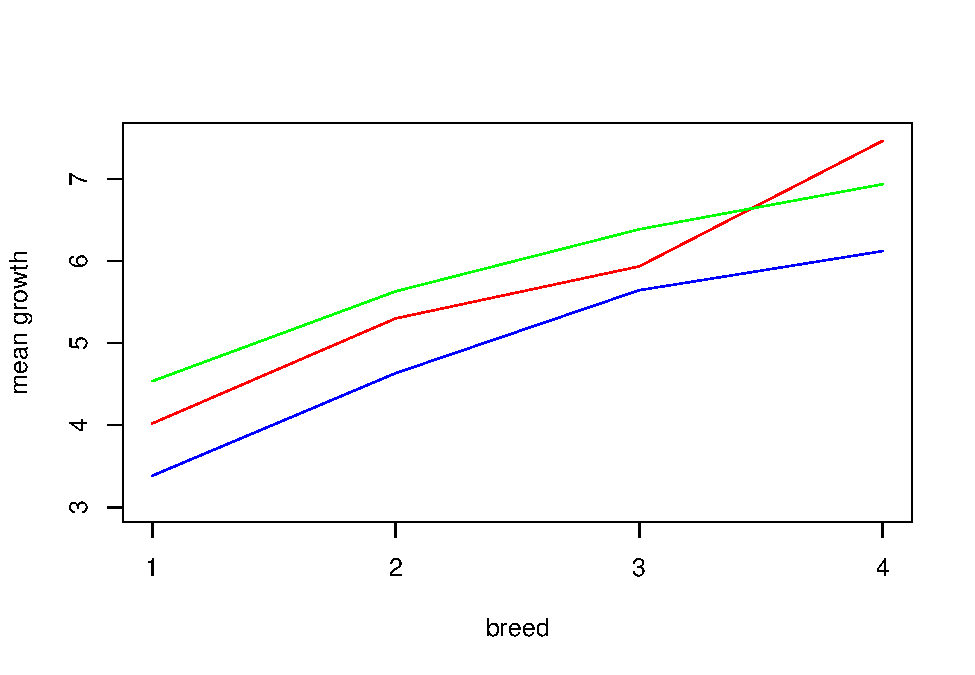
\includegraphics{11-StrategyForAnalysis_files/figure-latex/unnamed-chunk-6-1.pdf}

Given we can assume interactions are not present, let's test for main effects\ldots{} Ope, we already have these from the Type III SS ANOVA results above! Based on the p-values (\(\approx 0.014\) and \(0.000004\)), both main effects are significant. So, it makes sense to conduct follow-up tests based on factor-level means. I don't have any specific contrasts in mind to test, so I'll simply conduct pairwise comparisons.

Given it seems that breed and feed effects are additive/separable, the experimenters will likely make recommendations about breed and feed based on comparisons between levels of breeds and comparisons between levels of feed. Therefore, Tukey corrections for feed and for breed separately make the most sense. What I'm saying is that there are not likely to be decisions based on breed-feed comparisons jointly, so we can correct for comparing 3 pairs within feed and 6 pairs within breed separately.

Just for brevity, I'll only compute one Tukey-corrected pairwise comparison ``by hand''. Note, I match the p-value and the LS means computed using the emmeans package. However, I do not match the ``t.ratio'' in the table initially. The ``t.ratio'' in the table does not include the \(\frac{1}{\sqrt{2}}\) factor in the margin of error necessary for comparing to Tukey quantiles\ldots{} That's fine, just be careful you know exactly what you're looking at.

Based on the results, if the experimenters are interested in the breed and feed combinations with highest weight (which makes sense) then we see breed 4 has highest weight, and feeds 2 and 3 have higher weight than feed 1, although 2 and 3 are not distinguishable. The conclusion of this experiment is that feed and breed factors largely have additive effects on weight, and that breed 4 and feeds 2 and 3 seem to produce the highest weight chicks.

\begin{Shaded}
\begin{Highlighting}[]
\NormalTok{MSE }\OtherTok{\textless{}{-}}\NormalTok{ (SSE.full}\SpecialCharTok{/}\NormalTok{(n }\SpecialCharTok{{-}} \DecValTok{12}\NormalTok{))}


\NormalTok{means }\OtherTok{\textless{}{-}} \FunctionTok{aggregate}\NormalTok{(growth}\SpecialCharTok{\textasciitilde{}}\NormalTok{feed}\SpecialCharTok{*}\NormalTok{breed, }\AttributeTok{data =}\NormalTok{ chickgrowth, }\AttributeTok{FUN=}\NormalTok{mean)}
\NormalTok{LS.means.feed1 }\OtherTok{\textless{}{-}} \FloatTok{0.25}\SpecialCharTok{*}\NormalTok{(means[}\DecValTok{1}\NormalTok{,}\DecValTok{3}\NormalTok{]}\SpecialCharTok{+}\NormalTok{means[}\DecValTok{4}\NormalTok{,}\DecValTok{3}\NormalTok{]}\SpecialCharTok{+}\NormalTok{means[}\DecValTok{7}\NormalTok{,}\DecValTok{3}\NormalTok{]}\SpecialCharTok{+}\NormalTok{means[}\DecValTok{10}\NormalTok{,}\DecValTok{3}\NormalTok{])}
\NormalTok{n11 }\OtherTok{\textless{}{-}} \FunctionTok{sum}\NormalTok{(chickgrowth}\SpecialCharTok{$}\NormalTok{feed}\SpecialCharTok{==}\DecValTok{1} \SpecialCharTok{\&}\NormalTok{ chickgrowth}\SpecialCharTok{$}\NormalTok{breed}\SpecialCharTok{==}\DecValTok{1}\NormalTok{)}
\NormalTok{n12 }\OtherTok{\textless{}{-}} \FunctionTok{sum}\NormalTok{(chickgrowth}\SpecialCharTok{$}\NormalTok{feed}\SpecialCharTok{==}\DecValTok{1} \SpecialCharTok{\&}\NormalTok{ chickgrowth}\SpecialCharTok{$}\NormalTok{breed}\SpecialCharTok{==}\DecValTok{2}\NormalTok{)}
\NormalTok{n13 }\OtherTok{\textless{}{-}} \FunctionTok{sum}\NormalTok{(chickgrowth}\SpecialCharTok{$}\NormalTok{feed}\SpecialCharTok{==}\DecValTok{1} \SpecialCharTok{\&}\NormalTok{ chickgrowth}\SpecialCharTok{$}\NormalTok{breed}\SpecialCharTok{==}\DecValTok{3}\NormalTok{)}
\NormalTok{n14 }\OtherTok{\textless{}{-}} \FunctionTok{sum}\NormalTok{(chickgrowth}\SpecialCharTok{$}\NormalTok{feed}\SpecialCharTok{==}\DecValTok{1} \SpecialCharTok{\&}\NormalTok{ chickgrowth}\SpecialCharTok{$}\NormalTok{breed}\SpecialCharTok{==}\DecValTok{4}\NormalTok{)}
\NormalTok{LS.means.feed2 }\OtherTok{\textless{}{-}} \FloatTok{0.25}\SpecialCharTok{*}\NormalTok{(means[}\DecValTok{2}\NormalTok{,}\DecValTok{3}\NormalTok{]}\SpecialCharTok{+}\NormalTok{means[}\DecValTok{5}\NormalTok{,}\DecValTok{3}\NormalTok{]}\SpecialCharTok{+}\NormalTok{means[}\DecValTok{8}\NormalTok{,}\DecValTok{3}\NormalTok{]}\SpecialCharTok{+}\NormalTok{means[}\DecValTok{11}\NormalTok{,}\DecValTok{3}\NormalTok{])}
\NormalTok{n21 }\OtherTok{\textless{}{-}} \FunctionTok{sum}\NormalTok{(chickgrowth}\SpecialCharTok{$}\NormalTok{feed}\SpecialCharTok{==}\DecValTok{2} \SpecialCharTok{\&}\NormalTok{ chickgrowth}\SpecialCharTok{$}\NormalTok{breed}\SpecialCharTok{==}\DecValTok{1}\NormalTok{)}
\NormalTok{n22 }\OtherTok{\textless{}{-}} \FunctionTok{sum}\NormalTok{(chickgrowth}\SpecialCharTok{$}\NormalTok{feed}\SpecialCharTok{==}\DecValTok{2} \SpecialCharTok{\&}\NormalTok{ chickgrowth}\SpecialCharTok{$}\NormalTok{breed}\SpecialCharTok{==}\DecValTok{2}\NormalTok{)}
\NormalTok{n23 }\OtherTok{\textless{}{-}} \FunctionTok{sum}\NormalTok{(chickgrowth}\SpecialCharTok{$}\NormalTok{feed}\SpecialCharTok{==}\DecValTok{2} \SpecialCharTok{\&}\NormalTok{ chickgrowth}\SpecialCharTok{$}\NormalTok{breed}\SpecialCharTok{==}\DecValTok{3}\NormalTok{)}
\NormalTok{n24 }\OtherTok{\textless{}{-}} \FunctionTok{sum}\NormalTok{(chickgrowth}\SpecialCharTok{$}\NormalTok{feed}\SpecialCharTok{==}\DecValTok{2} \SpecialCharTok{\&}\NormalTok{ chickgrowth}\SpecialCharTok{$}\NormalTok{breed}\SpecialCharTok{==}\DecValTok{4}\NormalTok{)}


\NormalTok{tukey.feed12 }\OtherTok{\textless{}{-}}\NormalTok{ (LS.means.feed1}\SpecialCharTok{{-}}\NormalTok{LS.means.feed2) }\SpecialCharTok{/}\NormalTok{ ((}\DecValTok{1}\SpecialCharTok{/}\FunctionTok{sqrt}\NormalTok{(}\DecValTok{2}\NormalTok{))}\SpecialCharTok{*}\FunctionTok{sqrt}\NormalTok{(MSE}\SpecialCharTok{*}\NormalTok{(}\DecValTok{1}\SpecialCharTok{/}\DecValTok{16}\NormalTok{)}\SpecialCharTok{*}\NormalTok{(}\DecValTok{1}\SpecialCharTok{/}\NormalTok{n11}\SpecialCharTok{+}\DecValTok{1}\SpecialCharTok{/}\NormalTok{n12 }\SpecialCharTok{+} \DecValTok{1}\SpecialCharTok{/}\NormalTok{n13 }\SpecialCharTok{+} \DecValTok{1}\SpecialCharTok{/}\NormalTok{n14}\SpecialCharTok{+}\DecValTok{1}\SpecialCharTok{/}\NormalTok{n21}\SpecialCharTok{+}\DecValTok{1}\SpecialCharTok{/}\NormalTok{n22 }\SpecialCharTok{+} \DecValTok{1}\SpecialCharTok{/}\NormalTok{n23 }\SpecialCharTok{+} \DecValTok{1}\SpecialCharTok{/}\NormalTok{n24)))}

\NormalTok{tukey.feed12}
\end{Highlighting}
\end{Shaded}

\begin{verbatim}
## [1] -5.802434
\end{verbatim}

\begin{Shaded}
\begin{Highlighting}[]
\DecValTok{1}\SpecialCharTok{{-}}\FunctionTok{ptukey}\NormalTok{(}\FunctionTok{abs}\NormalTok{(tukey.feed12), }\DecValTok{3}\NormalTok{, n}\DecValTok{{-}12}\NormalTok{)}
\end{Highlighting}
\end{Shaded}

\begin{verbatim}
## [1] 0.002031653
\end{verbatim}

\begin{Shaded}
\begin{Highlighting}[]
\NormalTok{t.ratio }\OtherTok{\textless{}{-}}\NormalTok{ (LS.means.feed1}\SpecialCharTok{{-}}\NormalTok{LS.means.feed2) }\SpecialCharTok{/}\NormalTok{ (}\FunctionTok{sqrt}\NormalTok{(MSE}\SpecialCharTok{*}\NormalTok{(}\DecValTok{1}\SpecialCharTok{/}\DecValTok{16}\NormalTok{)}\SpecialCharTok{*}\NormalTok{(}\DecValTok{1}\SpecialCharTok{/}\NormalTok{n11}\SpecialCharTok{+}\DecValTok{1}\SpecialCharTok{/}\NormalTok{n12 }\SpecialCharTok{+} \DecValTok{1}\SpecialCharTok{/}\NormalTok{n13 }\SpecialCharTok{+} \DecValTok{1}\SpecialCharTok{/}\NormalTok{n14}\SpecialCharTok{+}\DecValTok{1}\SpecialCharTok{/}\NormalTok{n21}\SpecialCharTok{+}\DecValTok{1}\SpecialCharTok{/}\NormalTok{n22 }\SpecialCharTok{+} \DecValTok{1}\SpecialCharTok{/}\NormalTok{n23 }\SpecialCharTok{+} \DecValTok{1}\SpecialCharTok{/}\NormalTok{n24)))}

\NormalTok{t.ratio}
\end{Highlighting}
\end{Shaded}

\begin{verbatim}
## [1] -4.10294
\end{verbatim}

\begin{Shaded}
\begin{Highlighting}[]
\FunctionTok{library}\NormalTok{(emmeans)}
\NormalTok{em.feed }\OtherTok{\textless{}{-}} \FunctionTok{emmeans}\NormalTok{(}\FunctionTok{lm}\NormalTok{(growth}\SpecialCharTok{\textasciitilde{}}\NormalTok{feed}\SpecialCharTok{*}\NormalTok{breed, }\AttributeTok{data =}\NormalTok{ chickgrowth), }\FunctionTok{c}\NormalTok{(}\StringTok{\textquotesingle{}feed\textquotesingle{}}\NormalTok{))}
\end{Highlighting}
\end{Shaded}

\begin{verbatim}
## NOTE: Results may be misleading due to involvement in interactions
\end{verbatim}

\begin{Shaded}
\begin{Highlighting}[]
\NormalTok{em.feed}
\end{Highlighting}
\end{Shaded}

\begin{verbatim}
##  feed emmean    SE df lower.CL upper.CL
##  1      4.95 0.135 17     4.66     5.23
##  2      5.68 0.117 17     5.43     5.93
##  3      5.87 0.135 17     5.59     6.16
## 
## Results are averaged over the levels of: breed 
## Confidence level used: 0.95
\end{verbatim}

\begin{Shaded}
\begin{Highlighting}[]
\FunctionTok{pairs}\NormalTok{(em.feed, }\AttributeTok{adjust =} \StringTok{\textquotesingle{}tukey\textquotesingle{}}\NormalTok{)}
\end{Highlighting}
\end{Shaded}

\begin{verbatim}
##  contrast      estimate    SE df t.ratio p.value
##  feed1 - feed2   -0.734 0.179 17  -4.103  0.0020
##  feed1 - feed3   -0.926 0.191 17  -4.842  0.0004
##  feed2 - feed3   -0.192 0.179 17  -1.073  0.5427
## 
## Results are averaged over the levels of: breed 
## P value adjustment: tukey method for comparing a family of 3 estimates
\end{verbatim}

\begin{Shaded}
\begin{Highlighting}[]
\NormalTok{em.breed }\OtherTok{\textless{}{-}} \FunctionTok{emmeans}\NormalTok{(}\FunctionTok{lm}\NormalTok{(growth}\SpecialCharTok{\textasciitilde{}}\NormalTok{feed}\SpecialCharTok{*}\NormalTok{breed, }\AttributeTok{data =}\NormalTok{ chickgrowth), }\FunctionTok{c}\NormalTok{(}\StringTok{\textquotesingle{}breed\textquotesingle{}}\NormalTok{))}
\end{Highlighting}
\end{Shaded}

\begin{verbatim}
## NOTE: Results may be misleading due to involvement in interactions
\end{verbatim}

\begin{Shaded}
\begin{Highlighting}[]
\NormalTok{em.breed}
\end{Highlighting}
\end{Shaded}

\begin{verbatim}
##  breed emmean    SE df lower.CL upper.CL
##  1       3.98 0.147 17     3.67     4.29
##  2       5.19 0.138 17     4.90     5.48
##  3       5.99 0.138 17     5.70     6.28
##  4       6.84 0.173 17     6.48     7.20
## 
## Results are averaged over the levels of: feed 
## Confidence level used: 0.95
\end{verbatim}

\begin{Shaded}
\begin{Highlighting}[]
\FunctionTok{pairs}\NormalTok{(em.breed, }\AttributeTok{adjust =} \StringTok{\textquotesingle{}tukey\textquotesingle{}}\NormalTok{)}
\end{Highlighting}
\end{Shaded}

\begin{verbatim}
##  contrast        estimate    SE df t.ratio p.value
##  breed1 - breed2   -1.208 0.202 17  -5.993  0.0001
##  breed1 - breed3   -2.008 0.202 17  -9.957  <.0001
##  breed1 - breed4   -2.860 0.227 17 -12.603  <.0001
##  breed2 - breed3   -0.799 0.195 17  -4.104  0.0037
##  breed2 - breed4   -1.652 0.221 17  -7.478  <.0001
##  breed3 - breed4   -0.852 0.221 17  -3.858  0.0063
## 
## Results are averaged over the levels of: feed 
## P value adjustment: tukey method for comparing a family of 4 estimates
\end{verbatim}

\hypertarget{example-observational-study-on-growth-hormone-deficient-children-with-empty-cell}{%
\section{Example: observational study on growth-hormone deficient children with empty cell}\label{example-observational-study-on-growth-hormone-deficient-children-with-empty-cell}}

From Applied Linear Statistical Models (Fifth Edition) by Kutner et al.:
``Synthetic growth hormone was administered at a cI inical research center to growth hormone deficient, short children who had not yet reached pubel1y. The investigator was interested in the effects of a child's gender (Factor A) and bone development (Factor B) on the rate of growth induced by hormone administration. A child's bone development was classified into one of three categories: severely depressed, moderately depressed, mildly depressed. Three children were randomly selected for each gender-bone development group. The response variable (Y) of interest was the difference between the growth rate during growth hormone treatment and the normal growth rate prior to the treatment, expressed in centimeters per month. Four of the 18 children were unable to complete the year-long study, thus creating unequal treatment sample sizes. Note that this is an observational study. All children received the same hormone therapy, and, subsequently, changes in growth rates were observed for children in each bone development-by-gender category. No randomization of treatments to subjects was employed.''
We will examine a modified data set where an additional (fifth) response is missing so that we have an empty cell; in particular, the Female-Severely depressed combination is unobserved.

\begin{longtable}[]{@{}lll@{}}
\toprule()
Sex & Bone Development Depression & Mean(n) \\
\midrule()
\endhead
Male & Severe & 2.0(3) \\
Male & Moderate & 1.9(2) \\
Male & Mild & 0.9(2) \\
Female & Severe & -- \\
Female & Moderate & 2.1(3) \\
Female & Mild & 0.9(3) \\
\bottomrule()
\end{longtable}

\begin{Shaded}
\begin{Highlighting}[]
\NormalTok{response }\OtherTok{\textless{}{-}} \FunctionTok{c}\NormalTok{(}\FloatTok{1.4}\NormalTok{,}\FloatTok{2.4}\NormalTok{,}\FloatTok{2.2}\NormalTok{,}\FloatTok{2.1}\NormalTok{,}\FloatTok{1.7}\NormalTok{,}\FloatTok{0.7}\NormalTok{,}\FloatTok{1.1}\NormalTok{,}\FloatTok{2.5}\NormalTok{,}\FloatTok{1.8}\NormalTok{,}\FloatTok{2.0}\NormalTok{,}\FloatTok{0.5}\NormalTok{,}\FloatTok{0.9}\NormalTok{,}\FloatTok{1.3}\NormalTok{)}
\NormalTok{bone }\OtherTok{\textless{}{-}} \FunctionTok{c}\NormalTok{(}\StringTok{\textquotesingle{}severe\textquotesingle{}}\NormalTok{,}\StringTok{\textquotesingle{}severe\textquotesingle{}}\NormalTok{,}\StringTok{\textquotesingle{}severe\textquotesingle{}}\NormalTok{,}\StringTok{\textquotesingle{}moderate\textquotesingle{}}\NormalTok{,}\StringTok{\textquotesingle{}moderate\textquotesingle{}}\NormalTok{,}\StringTok{\textquotesingle{}mild\textquotesingle{}}\NormalTok{,}\StringTok{\textquotesingle{}mild\textquotesingle{}}\NormalTok{,}\StringTok{\textquotesingle{}moderate\textquotesingle{}}\NormalTok{,}\StringTok{\textquotesingle{}moderate\textquotesingle{}}\NormalTok{,}\StringTok{\textquotesingle{}moderate\textquotesingle{}}\NormalTok{,}\StringTok{\textquotesingle{}mild\textquotesingle{}}\NormalTok{,}\StringTok{\textquotesingle{}mild\textquotesingle{}}\NormalTok{,}\StringTok{\textquotesingle{}mild\textquotesingle{}}\NormalTok{)}
\NormalTok{sex }\OtherTok{\textless{}{-}} \FunctionTok{c}\NormalTok{(}\StringTok{\textquotesingle{}male\textquotesingle{}}\NormalTok{,}\StringTok{\textquotesingle{}male\textquotesingle{}}\NormalTok{,}\StringTok{\textquotesingle{}male\textquotesingle{}}\NormalTok{,}\StringTok{\textquotesingle{}male\textquotesingle{}}\NormalTok{,}\StringTok{\textquotesingle{}male\textquotesingle{}}\NormalTok{,}\StringTok{\textquotesingle{}male\textquotesingle{}}\NormalTok{,}\StringTok{\textquotesingle{}male\textquotesingle{}}\NormalTok{,}\StringTok{\textquotesingle{}female\textquotesingle{}}\NormalTok{,}\StringTok{\textquotesingle{}female\textquotesingle{}}\NormalTok{,}\StringTok{\textquotesingle{}female\textquotesingle{}}\NormalTok{,}\StringTok{\textquotesingle{}female\textquotesingle{}}\NormalTok{,}\StringTok{\textquotesingle{}female\textquotesingle{}}\NormalTok{,}\StringTok{\textquotesingle{}female\textquotesingle{}}\NormalTok{)}
\NormalTok{growth }\OtherTok{\textless{}{-}} \FunctionTok{data.frame}\NormalTok{(}\AttributeTok{response =}\NormalTok{ response, }\AttributeTok{bone =}\NormalTok{ bone, }\AttributeTok{sex =}\NormalTok{ sex)}
\end{Highlighting}
\end{Shaded}

\hypertarget{linear-model-analysis-with-extra-constraint}{%
\subsection{Linear Model analysis with extra constraint}\label{linear-model-analysis-with-extra-constraint}}

If we impose sum-to-zero constraints, and remove the interaction corresponding to the missing cell, then we can analyze the available data using one linear model.
Since there are a total of 5 cell means, we should have 5 regression parameters, 1 intercept, 2 for bone, 1 for sex, and 1 interaction term. I have chosen to design my own interaction term, which contrasts the mal-female difference in the moderate bone group to the male female difference in the mild bone group. If there is no interaction, these differences should be the same (because they are additive in sex and bone effects). Specifically, the interaction term I am testing is
\[(\mu_{21}-\mu_{22}) - (\mu_{31} - \mu_{32})\]
where the first index \(i\) denotes sex (\(i=1\) male and \(i=2\) female) and the second index \(j\) denotes bone (\(j=1\) severe, \(j=2\) moderate, \(j = 3\) mild).

\begin{Shaded}
\begin{Highlighting}[]
\FunctionTok{options}\NormalTok{(}\AttributeTok{contrasts =} \FunctionTok{c}\NormalTok{(}\StringTok{\textquotesingle{}contr.sum\textquotesingle{}}\NormalTok{, }\StringTok{\textquotesingle{}contr.sum\textquotesingle{}}\NormalTok{))}
\NormalTok{X.full }\OtherTok{\textless{}{-}} \FunctionTok{model.matrix}\NormalTok{(response }\SpecialCharTok{\textasciitilde{}}\NormalTok{ bone}\SpecialCharTok{*}\NormalTok{sex, }\AttributeTok{data =}\NormalTok{ growth)}
\NormalTok{X.obs }\OtherTok{\textless{}{-}}\NormalTok{ X.full[,}\DecValTok{1}\SpecialCharTok{:}\DecValTok{4}\NormalTok{]}
\NormalTok{X.obs }\OtherTok{\textless{}{-}} \FunctionTok{cbind}\NormalTok{(X.obs,}\FunctionTok{c}\NormalTok{(}\DecValTok{0}\NormalTok{,}\DecValTok{0}\NormalTok{,}\DecValTok{0}\NormalTok{,}\DecValTok{1}\NormalTok{,}\DecValTok{1}\NormalTok{,}\SpecialCharTok{{-}}\DecValTok{1}\NormalTok{,}\SpecialCharTok{{-}}\DecValTok{1}\NormalTok{,}\SpecialCharTok{{-}}\DecValTok{1}\NormalTok{,}\SpecialCharTok{{-}}\DecValTok{1}\NormalTok{,}\SpecialCharTok{{-}}\DecValTok{1}\NormalTok{,}\DecValTok{1}\NormalTok{,}\DecValTok{1}\NormalTok{,}\DecValTok{1}\NormalTok{))}
\FunctionTok{solve}\NormalTok{(}\FunctionTok{t}\NormalTok{(X.obs)}\SpecialCharTok{\%*\%}\NormalTok{X.obs)}\SpecialCharTok{\%*\%}\FunctionTok{t}\NormalTok{(X.obs)}
\end{Highlighting}
\end{Shaded}

\begin{verbatim}
##                         1             2             3           4           5
## (Intercept)  1.111111e-01  1.111111e-01  1.111111e-01  0.04166667  0.04166667
## bone1       -1.111111e-01 -1.111111e-01 -1.111111e-01 -0.04166667 -0.04166667
## bone2       -1.111111e-01 -1.111111e-01 -1.111111e-01  0.20833333  0.20833333
## sex1         1.387779e-17  1.387779e-17  1.387779e-17 -0.12500000 -0.12500000
##              0.000000e+00  0.000000e+00  0.000000e+00  0.12500000  0.12500000
##                       6           7           8           9          10
## (Intercept)  0.04166667  0.04166667  0.08333333  0.08333333  0.08333333
## bone1        0.20833333  0.20833333 -0.08333333 -0.08333333 -0.08333333
## bone2       -0.04166667 -0.04166667  0.08333333  0.08333333  0.08333333
## sex1        -0.12500000 -0.12500000  0.08333333  0.08333333  0.08333333
##             -0.12500000 -0.12500000 -0.08333333 -0.08333333 -0.08333333
##                      11          12          13
## (Intercept)  0.08333333  0.08333333  0.08333333
## bone1        0.08333333  0.08333333  0.08333333
## bone2       -0.08333333 -0.08333333 -0.08333333
## sex1         0.08333333  0.08333333  0.08333333
##              0.08333333  0.08333333  0.08333333
\end{verbatim}

Using this design I can test for interaction using a partial F test. The p-value is 0.711 which implies there is no significant interaction. Be careful about what this test is saying. The interaction term compares responses over sex and mild to moderate bone development disorder. Since we lack data for female-severe, we cannot say whether or not some interaction may occur for that level of bone development disorder.

\begin{Shaded}
\begin{Highlighting}[]
\NormalTok{n }\OtherTok{\textless{}{-}} \FunctionTok{nrow}\NormalTok{(X.obs)}
\NormalTok{p }\OtherTok{\textless{}{-}} \FunctionTok{ncol}\NormalTok{(X.obs)}
\NormalTok{hat.beta }\OtherTok{\textless{}{-}} \FunctionTok{solve}\NormalTok{(}\FunctionTok{t}\NormalTok{(X.obs)}\SpecialCharTok{\%*\%}\NormalTok{X.obs)}\SpecialCharTok{\%*\%}\FunctionTok{t}\NormalTok{(X.obs)}\SpecialCharTok{\%*\%}\FunctionTok{matrix}\NormalTok{(response, n,}\DecValTok{1}\NormalTok{)}
\NormalTok{hat.beta}
\end{Highlighting}
\end{Shaded}

\begin{verbatim}
##              [,1]
## (Intercept)  1.65
## bone1       -0.75
## bone2        0.35
## sex1         0.05
##             -0.05
\end{verbatim}

\begin{Shaded}
\begin{Highlighting}[]
\NormalTok{SSE.obs }\OtherTok{\textless{}{-}} \FunctionTok{sum}\NormalTok{((}\FunctionTok{matrix}\NormalTok{(response, n,}\DecValTok{1}\NormalTok{) }\SpecialCharTok{{-}}\NormalTok{ X.obs}\SpecialCharTok{\%*\%}\NormalTok{hat.beta)}\SpecialCharTok{\^{}}\DecValTok{2}\NormalTok{)}
\NormalTok{X.nointeraction }\OtherTok{\textless{}{-}}\NormalTok{ X.obs[,}\DecValTok{1}\SpecialCharTok{:}\DecValTok{4}\NormalTok{]}
\NormalTok{hat.beta.nointer }\OtherTok{\textless{}{-}} \FunctionTok{solve}\NormalTok{(}\FunctionTok{t}\NormalTok{(X.nointeraction)}\SpecialCharTok{\%*\%}\NormalTok{X.nointeraction)}\SpecialCharTok{\%*\%}\FunctionTok{t}\NormalTok{(X.nointeraction)}\SpecialCharTok{\%*\%}\FunctionTok{matrix}\NormalTok{(response, n,}\DecValTok{1}\NormalTok{)}
\NormalTok{SSE.nointer }\OtherTok{\textless{}{-}} \FunctionTok{sum}\NormalTok{((}\FunctionTok{matrix}\NormalTok{(response, n,}\DecValTok{1}\NormalTok{) }\SpecialCharTok{{-}}\NormalTok{ X.nointeraction}\SpecialCharTok{\%*\%}\NormalTok{hat.beta.nointer)}\SpecialCharTok{\^{}}\DecValTok{2}\NormalTok{)}

\NormalTok{F }\OtherTok{\textless{}{-}}\NormalTok{ ((SSE.nointer }\SpecialCharTok{{-}}\NormalTok{ SSE.obs)}\SpecialCharTok{/}\DecValTok{1}\NormalTok{)}\SpecialCharTok{/}\NormalTok{(SSE.obs}\SpecialCharTok{/}\NormalTok{(n}\SpecialCharTok{{-}}\NormalTok{p))}
\NormalTok{F}
\end{Highlighting}
\end{Shaded}

\begin{verbatim}
## [1] 0.1476923
\end{verbatim}

\begin{Shaded}
\begin{Highlighting}[]
\DecValTok{1}\SpecialCharTok{{-}}\FunctionTok{pf}\NormalTok{(F,}\DecValTok{1}\NormalTok{,n}\SpecialCharTok{{-}}\NormalTok{p)}
\end{Highlighting}
\end{Shaded}

\begin{verbatim}
## [1] 0.7107643
\end{verbatim}

Given the only testable interaction is not significant, we move on to examining the main effects. The first estimated main effect for bone is given by\\
\[-1/9Y_1 -1/9Y_2 -1/9Y_3  -1/24Y_4 - 1/24Y_5  +5/24Y_6 + 5/24Y_7 -1/12Y_8 - 1/12Y_9 - 1/12Y_10 + 1/12Y_11 + 1/12Y_12 + 1/12Y_13.\]
This is an estimate of the following contrast:
\[-1/3\mu_{11}-1/12\mu_{21}+5/12\mu_{31}  +    1/4(\mu_{22}-\mu_{32})\]
The difference \(\mu_{22}-\mu_{32}\) is the difference in mean response for females in groups moderate and mild. If there is no difference between bone groups (no bone effects) then this difference should be zero because both are average female responses. Likewise, if there are no bone effects, then \(-1/3\mu_{11}-1/12\mu_{21}+5/12\mu_{31}\) simplifies to a linear combination of \(\mu_\cdot 1\), the average male response; and that linear combination is \(-1/3\mu_{\cdot 1}-1/12\mu_{\cdot 1}+5/12\mu_{\cdot 1} = 0\).

The partial F test for bone effect is significant; there are significant difference in mean growth between treated and untreated periods depending on one's severity of bone under-development.

\begin{Shaded}
\begin{Highlighting}[]
\NormalTok{X.nobone }\OtherTok{\textless{}{-}}\NormalTok{ X.obs[,}\SpecialCharTok{{-}}\NormalTok{(}\DecValTok{2}\SpecialCharTok{:}\DecValTok{3}\NormalTok{)]}
\NormalTok{hat.beta.nobone }\OtherTok{\textless{}{-}} \FunctionTok{solve}\NormalTok{(}\FunctionTok{t}\NormalTok{(X.nobone)}\SpecialCharTok{\%*\%}\NormalTok{X.nobone)}\SpecialCharTok{\%*\%}\FunctionTok{t}\NormalTok{(X.nobone)}\SpecialCharTok{\%*\%}\FunctionTok{matrix}\NormalTok{(response, n,}\DecValTok{1}\NormalTok{)}
\NormalTok{SSE.nobone }\OtherTok{\textless{}{-}} \FunctionTok{sum}\NormalTok{((}\FunctionTok{matrix}\NormalTok{(response, n,}\DecValTok{1}\NormalTok{) }\SpecialCharTok{{-}}\NormalTok{ X.nobone}\SpecialCharTok{\%*\%}\NormalTok{hat.beta.nobone)}\SpecialCharTok{\^{}}\DecValTok{2}\NormalTok{)}

\NormalTok{F }\OtherTok{\textless{}{-}}\NormalTok{ ((SSE.nobone }\SpecialCharTok{{-}}\NormalTok{ SSE.obs)}\SpecialCharTok{/}\DecValTok{2}\NormalTok{)}\SpecialCharTok{/}\NormalTok{(SSE.obs}\SpecialCharTok{/}\NormalTok{(n}\SpecialCharTok{{-}}\NormalTok{p))}
\NormalTok{F}
\end{Highlighting}
\end{Shaded}

\begin{verbatim}
## [1] 10.83429
\end{verbatim}

\begin{Shaded}
\begin{Highlighting}[]
\DecValTok{1}\SpecialCharTok{{-}}\FunctionTok{pf}\NormalTok{(F,}\DecValTok{1}\NormalTok{,n}\SpecialCharTok{{-}}\NormalTok{p)}
\end{Highlighting}
\end{Shaded}

\begin{verbatim}
## [1] 0.01099661
\end{verbatim}

There is not a significant difference in mean bone growth between sexes.

\begin{Shaded}
\begin{Highlighting}[]
\NormalTok{X.nosex }\OtherTok{\textless{}{-}}\NormalTok{ X.obs[,}\SpecialCharTok{{-}}\DecValTok{4}\NormalTok{]}
\NormalTok{hat.beta.nosex }\OtherTok{\textless{}{-}} \FunctionTok{solve}\NormalTok{(}\FunctionTok{t}\NormalTok{(X.nosex)}\SpecialCharTok{\%*\%}\NormalTok{X.nosex)}\SpecialCharTok{\%*\%}\FunctionTok{t}\NormalTok{(X.nosex)}\SpecialCharTok{\%*\%}\FunctionTok{matrix}\NormalTok{(response, n,}\DecValTok{1}\NormalTok{)}
\NormalTok{SSE.nosex }\OtherTok{\textless{}{-}} \FunctionTok{sum}\NormalTok{((}\FunctionTok{matrix}\NormalTok{(response, n,}\DecValTok{1}\NormalTok{) }\SpecialCharTok{{-}}\NormalTok{ X.nosex}\SpecialCharTok{\%*\%}\NormalTok{hat.beta.nosex)}\SpecialCharTok{\^{}}\DecValTok{2}\NormalTok{)}

\NormalTok{F }\OtherTok{\textless{}{-}}\NormalTok{ ((SSE.nosex }\SpecialCharTok{{-}}\NormalTok{ SSE.obs)}\SpecialCharTok{/}\DecValTok{1}\NormalTok{)}\SpecialCharTok{/}\NormalTok{(SSE.obs}\SpecialCharTok{/}\NormalTok{(n}\SpecialCharTok{{-}}\NormalTok{p))}
\NormalTok{F}
\end{Highlighting}
\end{Shaded}

\begin{verbatim}
## [1] 0.1476923
\end{verbatim}

\begin{Shaded}
\begin{Highlighting}[]
\DecValTok{1}\SpecialCharTok{{-}}\FunctionTok{pf}\NormalTok{(F,}\DecValTok{1}\NormalTok{,n}\SpecialCharTok{{-}}\NormalTok{p)}
\end{Highlighting}
\end{Shaded}

\begin{verbatim}
## [1] 0.7107643
\end{verbatim}

Now, which means should we compare? Since only bone is significant we should compare the three bone under-development levels pairwise. However, we should consider whether or not it makes sense to compare the LS mean response for sever bone under-development considering it only contains male responses. In this case, since sex is not significant, I think it is reasonable to make comparisons of severe to moderate and severe to mild. However, if sex was significant, then such comparisons would not make sense as there would be no females to average over within the severe category.'
The mild bone underdevelopment group is significantly different from the moderate and severe groups, but the latter two are not distinguishable.

\begin{Shaded}
\begin{Highlighting}[]
\NormalTok{MSE }\OtherTok{\textless{}{-}}\NormalTok{ SSE.obs}\SpecialCharTok{/}\NormalTok{(n}\SpecialCharTok{{-}}\NormalTok{p)}
\NormalTok{LS.bone }\OtherTok{\textless{}{-}} \FunctionTok{c}\NormalTok{(}\DecValTok{2}\NormalTok{,}\DecValTok{2}\NormalTok{,}\FloatTok{0.9}\NormalTok{)}
\NormalTok{ratio}\FloatTok{.12} \OtherTok{\textless{}{-}} \DecValTok{0}
\NormalTok{ratio}\FloatTok{.13} \OtherTok{\textless{}{-}} \FloatTok{1.1}\SpecialCharTok{/}\FunctionTok{sqrt}\NormalTok{(MSE}\SpecialCharTok{*}\NormalTok{(}\DecValTok{1}\SpecialCharTok{/}\DecValTok{2}\NormalTok{)}\SpecialCharTok{*}\NormalTok{(}\DecValTok{1}\SpecialCharTok{/}\DecValTok{3}\SpecialCharTok{+}\NormalTok{(}\DecValTok{1}\SpecialCharTok{/}\DecValTok{4}\NormalTok{)}\SpecialCharTok{*}\NormalTok{(}\DecValTok{1}\SpecialCharTok{/}\DecValTok{2}\SpecialCharTok{+}\DecValTok{1}\SpecialCharTok{/}\DecValTok{3}\NormalTok{)))}
\NormalTok{ratio}\FloatTok{.23} \OtherTok{\textless{}{-}} \FloatTok{1.1}\SpecialCharTok{/}\FunctionTok{sqrt}\NormalTok{(MSE}\SpecialCharTok{*}\NormalTok{(}\DecValTok{1}\SpecialCharTok{/}\DecValTok{2}\NormalTok{)}\SpecialCharTok{*}\NormalTok{(}\DecValTok{1}\SpecialCharTok{/}\DecValTok{4}\NormalTok{)}\SpecialCharTok{*}\NormalTok{(}\DecValTok{1}\SpecialCharTok{/}\DecValTok{2}\SpecialCharTok{+}\DecValTok{1}\SpecialCharTok{/}\DecValTok{3}\SpecialCharTok{+}\DecValTok{1}\SpecialCharTok{/}\DecValTok{2}\SpecialCharTok{+}\DecValTok{1}\SpecialCharTok{/}\DecValTok{3}\NormalTok{))}

\NormalTok{p12 }\OtherTok{\textless{}{-}} \DecValTok{1}\SpecialCharTok{{-}}\FunctionTok{ptukey}\NormalTok{(ratio}\FloatTok{.12}\NormalTok{, }\DecValTok{3}\NormalTok{, n}\SpecialCharTok{{-}}\NormalTok{p)}
\NormalTok{p12}
\end{Highlighting}
\end{Shaded}

\begin{verbatim}
## [1] 1
\end{verbatim}

\begin{Shaded}
\begin{Highlighting}[]
\NormalTok{p13 }\OtherTok{\textless{}{-}} \DecValTok{1}\SpecialCharTok{{-}}\FunctionTok{ptukey}\NormalTok{(ratio}\FloatTok{.13}\NormalTok{, }\DecValTok{3}\NormalTok{, n}\SpecialCharTok{{-}}\NormalTok{p)}
\NormalTok{p13}
\end{Highlighting}
\end{Shaded}

\begin{verbatim}
## [1] 0.01467942
\end{verbatim}

\begin{Shaded}
\begin{Highlighting}[]
\NormalTok{p23 }\OtherTok{\textless{}{-}} \DecValTok{1}\SpecialCharTok{{-}}\FunctionTok{ptukey}\NormalTok{(ratio}\FloatTok{.23}\NormalTok{, }\DecValTok{3}\NormalTok{, n}\SpecialCharTok{{-}}\NormalTok{p)}
\NormalTok{p23}
\end{Highlighting}
\end{Shaded}

\begin{verbatim}
## [1] 0.00720332
\end{verbatim}

\hypertarget{partial-table-analysis}{%
\subsection{Partial Table analysis}\label{partial-table-analysis}}

An alternative strategy is to consider partial table analyses. On table consists of male and female at levels moderate and mild. The second, overlapping table is all male cells (severe, moderate, mild). In the first, two-by-two table, we may assess interaction. If interaction is present, then we should compare all 5 cell means. If not, we test main effects to determine if male-female comparisons are relevant, and if moderate-mild comparisons are relevant. Using the second, three-by-one table of only male responses, we can compare severe-moderate-mild within males, if desired.

Below, we fit the linear model to the partial table of male-female, moderate-mild responses. The interaction term is given by
\[(\mu_{22}-\mu_{21}) - (\mu_{32}-\mu_{31})\]
which is the mean growth for (female:moderate - male:moderate)-(female:mild - male:mild). If there is no interaction, then the female to male difference is the same at levels moderate and mild, so this contrast of means would be equal to zero. Since the interaction is found to be insignificant, we move on to main effects.

As in the full data analysis above, sex is not significant. I think this fact makes it less clear, rather than more clear, how to proceed. Since sex is not significant and bone under-development is significant, it makes sense to compare mean responses between levels of the bone factor, averaged over sex (LS means). However, now we must choose which table to use. We can compare LS means in the \(2\times 2\) partial table, or in the \(3\times 1\) table of only male responses, or we can go back to the full data and compare LS means for the bone factor using all the data. The third option matches the full data analysis from above, and makes sense given that sex is not significant. One advantage of the partial table analysis is that if sex is significant, it does not make sense to compare LS means of the bone factor because one of those contains no females; therefore, a partial table analysis seems necessary. In the present case, I would advocate for the full data analysis, comparing LS means of bone considering sex is not significant, in which case the rest of the analysis is the same as above.

\begin{Shaded}
\begin{Highlighting}[]
\NormalTok{growth2 }\OtherTok{\textless{}{-}}\NormalTok{ growth[}\DecValTok{4}\SpecialCharTok{:}\NormalTok{n,]}
\NormalTok{growth2}\SpecialCharTok{$}\NormalTok{bone }\OtherTok{=} \FunctionTok{factor}\NormalTok{(growth2}\SpecialCharTok{$}\NormalTok{bone, }\AttributeTok{levels =} \FunctionTok{unique}\NormalTok{(growth2}\SpecialCharTok{$}\NormalTok{bone))}
\FunctionTok{library}\NormalTok{(car)}
\NormalTok{my.lm}\OtherTok{\textless{}{-}}\FunctionTok{lm}\NormalTok{(response}\SpecialCharTok{\textasciitilde{}}\NormalTok{bone}\SpecialCharTok{*}\NormalTok{sex, }\AttributeTok{data =}\NormalTok{ growth2)}
\FunctionTok{Anova}\NormalTok{(my.lm)}
\end{Highlighting}
\end{Shaded}

\begin{verbatim}
## Anova Table (Type II tests)
## 
## Response: response
##           Sum Sq Df F value   Pr(>F)   
## bone       3.136  1 25.4270 0.002351 **
## sex        0.024  1  0.1946 0.674571   
## bone:sex   0.024  1  0.1946 0.674571   
## Residuals  0.740  6                    
## ---
## Signif. codes:  0 '***' 0.001 '**' 0.01 '*' 0.05 '.' 0.1 ' ' 1
\end{verbatim}

\begin{Shaded}
\begin{Highlighting}[]
\FunctionTok{summary}\NormalTok{(my.lm)}
\end{Highlighting}
\end{Shaded}

\begin{verbatim}
## 
## Call:
## lm(formula = response ~ bone * sex, data = growth2)
## 
## Residuals:
##    Min     1Q Median     3Q    Max 
##  -0.40  -0.20  -0.05   0.20   0.40 
## 
## Coefficients:
##             Estimate Std. Error t value Pr(>|t|)    
## (Intercept)   1.4500     0.1134  12.793  1.4e-05 ***
## bone1         0.5500     0.1134   4.852  0.00284 ** 
## sex1          0.0500     0.1134   0.441  0.67457    
## bone1:sex1    0.0500     0.1134   0.441  0.67457    
## ---
## Signif. codes:  0 '***' 0.001 '**' 0.01 '*' 0.05 '.' 0.1 ' ' 1
## 
## Residual standard error: 0.3512 on 6 degrees of freedom
## Multiple R-squared:  0.8114, Adjusted R-squared:  0.7171 
## F-statistic: 8.605 on 3 and 6 DF,  p-value: 0.01359
\end{verbatim}

\begin{Shaded}
\begin{Highlighting}[]
\NormalTok{X }\OtherTok{\textless{}{-}} \FunctionTok{model.matrix}\NormalTok{(response}\SpecialCharTok{\textasciitilde{}}\NormalTok{bone}\SpecialCharTok{*}\NormalTok{sex, }\AttributeTok{data =}\NormalTok{ growth2)}
\FunctionTok{solve}\NormalTok{(}\FunctionTok{t}\NormalTok{(X)}\SpecialCharTok{\%*\%}\NormalTok{X)}\SpecialCharTok{\%*\%}\FunctionTok{t}\NormalTok{(X)}
\end{Highlighting}
\end{Shaded}

\begin{verbatim}
##                  4      5      6      7          8          9         10
## (Intercept)  0.125  0.125  0.125  0.125 0.08333333 0.08333333 0.08333333
## bone1        0.125  0.125 -0.125 -0.125 0.08333333 0.08333333 0.08333333
## sex1        -0.125 -0.125 -0.125 -0.125 0.08333333 0.08333333 0.08333333
## bone1:sex1  -0.125 -0.125  0.125  0.125 0.08333333 0.08333333 0.08333333
##                      11          12          13
## (Intercept)  0.08333333  0.08333333  0.08333333
## bone1       -0.08333333 -0.08333333 -0.08333333
## sex1         0.08333333  0.08333333  0.08333333
## bone1:sex1  -0.08333333 -0.08333333 -0.08333333
\end{verbatim}

\hypertarget{k-factorial-experiments}{%
\chapter{\texorpdfstring{\(2^k\) Factorial Experiments}{2\^{}k Factorial Experiments}}\label{k-factorial-experiments}}

We will wrap up our discussion of ANOVA-type models with \(2^k\) factorial experiments. A study of \(k\) binary factors and their effects on a response is a \(2^k\) factorial experiment. The two distinguishing features of these experiments is the fact all factors have only two levels, and the large number of crossed treatments. These result in some unique challenges, but also some simplifications.

\hypertarget{the-model-1}{%
\section{The Model}\label{the-model-1}}

The ANOVa-type notation becomes cumbersome for \(2^k\) factorial experiments, so we favor the regression-type notation. For example, suppose \(k=3\) so that there are 8 crossed factors. We have main effects, and interactions involving 2, 3, or all 4 factors. To denote the corresponding parameters we use \(\beta_j\) for \(j=1, \ldots, 4\) for main effects, \(\beta_{jk}\) for two-way interactions, and \(\beta_{jk\ell}\) for three-way interactions. Then, using the subscript \(i\) for the observation \(\i = 1, \ldots, n\), the model can be written
\[Y_i = \beta_0 + \beta_1X_{1i}+\beta_2X_{2i}+\beta_3 X_{3i} + \beta_{12}X_{12i} + \beta_{13}X_{13i}+\beta_{23}X_{23i} + \beta_{123}X_{123i}+\epsilon_i.  \]
Note we have 8 regression coefficients corresponding to the 8 crossed treatment means.

For balanced experiments some interesting simplifications emerge. The design matrix may be easily coded using a sum-to-zero format as follows. Let response \(i\) in main effects column \(j\) be -1 if it has the first level of the factor and +1 if it has the second level. Note that interaction columns of the design are determined by multiplication of the main effects columns. Suppose for \(k=3\) we have 16 responses (2 replicates for each combination of factor levels). The first column of \(X\) is all 1's. The second, third, and fourth columns are for main effects, adn the last four are for interactions. The design matrix is as follows:

\[\begin{matrix}
 1 & -1 & -1 & -1 &  1& 1& 1& -1 \\
 1 & -1 & -1 & -1 &  1& 1& 1& -1 \\
 1 & 1 & -1 & -1 &  -1& -1& 1& -1 \\
 1 & 1 & -1 & -1 &  -1& -1& 1& -1 \\
 1 & 1 & 1 & -1 &  1& -1& -1& -1 \\
 1 & 1 & 1 & -1 &  1& -1& -1& -1 \\
 1 & 1 & 1 & 1 &  1& 1& 1& 1 \\
 1 & 1 & 1 & 1 &  1& 1& 1& 1 \\
 1 & -1 & 1 & -1 &  -1& 1& -1& 1 \\
 1 & -1 & 1 & -1 &  -1& 1& -1& 1 \\
 1 & -1 & -1 & 1 &  1& -1& -1& 1 \\
 1 & -1 & -1 & 1 &  1& -1& -1& 1 \\
 1 & -1 & 1 & 1 &  -1& -1& 1& -1 \\
 1 & -1 & 1 & 1 &  -1& -1& 1& -1 \\
 1 & 1 & -1 & 1 &  -1& 1& -1& 1 \\
 1 & 1 & -1 & 1 &  -1& 1& -1& 1 \\
 \end{matrix}
\]

The design matrix \(X\) has the interesting property that any two columns are orthogonal, i.e., their inner (dot) product is zero. Therefore, \(X^\top X = 16 I_{16}\) and \((X^\top X)^{-1} = \frac{1}{16}I_{16}\). And, \(\hat\beta = \frac{1}{16}X^\top Y\), making computation of the estimated regression coefficients very easy. It also means that the estimated regression coefficients are uncorrelated (because \((X^\top X)^{-1}\) has all zeroes on the off-diagonals) with equal variance \(\sigma^2 / 16\) (because the diagonal entries are equal).

\hypertarget{example-stress-test-study}{%
\subsection{Example: Stress Test Study}\label{example-stress-test-study}}

The following data records the results of a stress test measuring exercise tolerance on male and female adults who smoke (light or heavy) and who have high or low body fat:

\begin{Shaded}
\begin{Highlighting}[]
\NormalTok{stress }\OtherTok{\textless{}{-}} \FunctionTok{c}\NormalTok{(}\FloatTok{24.1}\NormalTok{,}\FloatTok{29.2}\NormalTok{,}\FloatTok{24.6}\NormalTok{,}\FloatTok{20.0}\NormalTok{,}\FloatTok{21.9}\NormalTok{,}\FloatTok{17.6}\NormalTok{,}\FloatTok{14.6}\NormalTok{,}\FloatTok{15.3}\NormalTok{,}\FloatTok{12.3}\NormalTok{,}\FloatTok{16.1}\NormalTok{,}\FloatTok{9.3}\NormalTok{,}\FloatTok{10.8}\NormalTok{,}\FloatTok{17.6}\NormalTok{,}\FloatTok{18.8}\NormalTok{,}\FloatTok{23.2}\NormalTok{,}\FloatTok{14.8}\NormalTok{,}\FloatTok{10.3}\NormalTok{,}\FloatTok{11.3}\NormalTok{,}\FloatTok{14.9}\NormalTok{,}\FloatTok{20.4}\NormalTok{,}\FloatTok{12.8}\NormalTok{,}\FloatTok{10.1}\NormalTok{,}\FloatTok{14.4}\NormalTok{,}\FloatTok{6.1}\NormalTok{)}
\NormalTok{smoking }\OtherTok{\textless{}{-}}\FunctionTok{c}\NormalTok{(}\FunctionTok{rep}\NormalTok{(}\SpecialCharTok{{-}}\DecValTok{1}\NormalTok{,}\DecValTok{12}\NormalTok{), }\FunctionTok{rep}\NormalTok{(}\DecValTok{1}\NormalTok{,}\DecValTok{12}\NormalTok{))}
\NormalTok{fat }\OtherTok{\textless{}{-}} \FunctionTok{c}\NormalTok{(}\FunctionTok{rep}\NormalTok{(}\SpecialCharTok{{-}}\DecValTok{1}\NormalTok{,}\DecValTok{6}\NormalTok{), }\FunctionTok{rep}\NormalTok{(}\DecValTok{1}\NormalTok{,}\DecValTok{6}\NormalTok{),}\FunctionTok{rep}\NormalTok{(}\SpecialCharTok{{-}}\DecValTok{1}\NormalTok{,}\DecValTok{6}\NormalTok{), }\FunctionTok{rep}\NormalTok{(}\DecValTok{1}\NormalTok{,}\DecValTok{6}\NormalTok{))}
\NormalTok{sex }\OtherTok{\textless{}{-}} \FunctionTok{c}\NormalTok{(}\SpecialCharTok{{-}}\DecValTok{1}\NormalTok{,}\SpecialCharTok{{-}}\DecValTok{1}\NormalTok{,}\SpecialCharTok{{-}}\DecValTok{1}\NormalTok{,}\DecValTok{1}\NormalTok{,}\DecValTok{1}\NormalTok{,}\DecValTok{1}\NormalTok{,}\SpecialCharTok{{-}}\DecValTok{1}\NormalTok{,}\SpecialCharTok{{-}}\DecValTok{1}\NormalTok{,}\SpecialCharTok{{-}}\DecValTok{1}\NormalTok{,}\DecValTok{1}\NormalTok{,}\DecValTok{1}\NormalTok{,}\DecValTok{1}\NormalTok{,}\SpecialCharTok{{-}}\DecValTok{1}\NormalTok{,}\SpecialCharTok{{-}}\DecValTok{1}\NormalTok{,}\SpecialCharTok{{-}}\DecValTok{1}\NormalTok{,}\DecValTok{1}\NormalTok{,}\DecValTok{1}\NormalTok{,}\DecValTok{1}\NormalTok{,}\SpecialCharTok{{-}}\DecValTok{1}\NormalTok{,}\SpecialCharTok{{-}}\DecValTok{1}\NormalTok{,}\SpecialCharTok{{-}}\DecValTok{1}\NormalTok{,}\DecValTok{1}\NormalTok{,}\DecValTok{1}\NormalTok{,}\DecValTok{1}\NormalTok{)}
\NormalTok{data.df }\OtherTok{\textless{}{-}} \FunctionTok{data.frame}\NormalTok{(}\AttributeTok{stress =}\NormalTok{ stress, }\AttributeTok{smoking =} \FunctionTok{as.factor}\NormalTok{(smoking), }\AttributeTok{fat=}\FunctionTok{as.factor}\NormalTok{(fat), }\AttributeTok{sex=}\FunctionTok{as.factor}\NormalTok{(sex))}

\NormalTok{X }\OtherTok{\textless{}{-}} \FunctionTok{model.matrix}\NormalTok{(stress}\SpecialCharTok{\textasciitilde{}}\NormalTok{smoking}\SpecialCharTok{*}\NormalTok{fat}\SpecialCharTok{*}\NormalTok{sex, }\AttributeTok{data =}\NormalTok{ data.df)}

\FunctionTok{t}\NormalTok{(X)}\SpecialCharTok{\%*\%}\NormalTok{X}
\end{Highlighting}
\end{Shaded}

\begin{verbatim}
##                    (Intercept) smoking1 fat1 sex1 smoking1:fat1 smoking1:sex1
## (Intercept)                 24       12   12   12             6             6
## smoking1                    12       12    6    6             6             6
## fat1                        12        6   12    6             6             3
## sex1                        12        6    6   12             3             6
## smoking1:fat1                6        6    6    3             6             3
## smoking1:sex1                6        6    3    6             3             6
## fat1:sex1                    6        3    6    6             3             3
## smoking1:fat1:sex1           3        3    3    3             3             3
##                    fat1:sex1 smoking1:fat1:sex1
## (Intercept)                6                  3
## smoking1                   3                  3
## fat1                       6                  3
## sex1                       6                  3
## smoking1:fat1              3                  3
## smoking1:sex1              3                  3
## fat1:sex1                  6                  3
## smoking1:fat1:sex1         3                  3
\end{verbatim}

\begin{Shaded}
\begin{Highlighting}[]
\FunctionTok{solve}\NormalTok{(}\FunctionTok{t}\NormalTok{(X)}\SpecialCharTok{\%*\%}\NormalTok{X)}\SpecialCharTok{\%*\%}\FunctionTok{t}\NormalTok{(X)}\SpecialCharTok{\%*\%}\FunctionTok{matrix}\NormalTok{(stress,}\DecValTok{24}\NormalTok{,}\DecValTok{1}\NormalTok{)}
\end{Highlighting}
\end{Shaded}

\begin{verbatim}
##                          [,1]
## (Intercept)         25.966667
## smoking1            -6.100000
## fat1               -11.900000
## sex1                -6.133333
## smoking1:fat1        8.066667
## smoking1:sex1       -1.600000
## fat1:sex1            4.133333
## smoking1:fat1:sex1  -2.233333
\end{verbatim}

\begin{Shaded}
\begin{Highlighting}[]
\FunctionTok{lm}\NormalTok{(stress}\SpecialCharTok{\textasciitilde{}}\NormalTok{smoking}\SpecialCharTok{*}\NormalTok{fat}\SpecialCharTok{*}\NormalTok{sex, }\AttributeTok{data =}\NormalTok{ data.df)}
\end{Highlighting}
\end{Shaded}

\begin{verbatim}
## 
## Call:
## lm(formula = stress ~ smoking * fat * sex, data = data.df)
## 
## Coefficients:
##        (Intercept)            smoking1                fat1                sex1  
##             25.967              -6.100             -11.900              -6.133  
##      smoking1:fat1       smoking1:sex1           fat1:sex1  smoking1:fat1:sex1  
##              8.067              -1.600               4.133              -2.233
\end{verbatim}

\begin{Shaded}
\begin{Highlighting}[]
\FunctionTok{summary}\NormalTok{(}\FunctionTok{lm}\NormalTok{(stress}\SpecialCharTok{\textasciitilde{}}\NormalTok{smoking}\SpecialCharTok{*}\NormalTok{fat}\SpecialCharTok{*}\NormalTok{sex, }\AttributeTok{data =}\NormalTok{ data.df))}
\end{Highlighting}
\end{Shaded}

\begin{verbatim}
## 
## Call:
## lm(formula = stress ~ smoking * fat * sex, data = data.df)
## 
## Residuals:
##    Min     1Q Median     3Q    Max 
## -4.100 -1.842 -0.950  2.217  4.367 
## 
## Coefficients:
##                    Estimate Std. Error t value Pr(>|t|)    
## (Intercept)          25.967      1.764  14.720 1.01e-10 ***
## smoking1             -6.100      2.495  -2.445 0.026427 *  
## fat1                -11.900      2.495  -4.770 0.000209 ***
## sex1                 -6.133      2.495  -2.459 0.025730 *  
## smoking1:fat1         8.067      3.528   2.286 0.036198 *  
## smoking1:sex1        -1.600      3.528  -0.454 0.656274    
## fat1:sex1             4.133      3.528   1.172 0.258526    
## smoking1:fat1:sex1   -2.233      4.989  -0.448 0.660434    
## ---
## Signif. codes:  0 '***' 0.001 '**' 0.01 '*' 0.05 '.' 0.1 ' ' 1
## 
## Residual standard error: 3.055 on 16 degrees of freedom
## Multiple R-squared:  0.7976, Adjusted R-squared:  0.709 
## F-statistic: 9.007 on 7 and 16 DF,  p-value: 0.0001525
\end{verbatim}

\hypertarget{unreplicated-factorial-experiments}{%
\section{Unreplicated Factorial Experiments}\label{unreplicated-factorial-experiments}}

Often, in practice, \(k\) is very large, so that not enough sample size is available to run a replicated experiment. When only 1 response is available for each crossed treatment (i.e.~\(n = 2^k\)), the \(2^k\) factorial experiment is called ``unreplicated'', and no degrees of freedom are available to estimate the variance \(\sigma^2\).

In unreplicated experiments, there are a few strategies available for recovering an estimate of \(\sigma^2\).
1. We can simply assume some interactions (usually higher-order first) are zero, and then the degrees of freedom associated with these may be put towards estimating \(\sigma^2\).
2. Graphical methods (Pareto plots).
3. Center-point replication.

The Pareto plot is a graphical display showing the ratio of effect sum of squares to total sum of squares where effect sum of squares is \(n\hat\beta_j^2\) for each of the \(2^k\) coefficients. A common technique is to use the effects with smallest sums of squares to pool to obtain a variance estimate. The resulting variance estimate is likely to be an underestimate.

Center-point replication is sometimes implementable for factors based on underlying continuous variables. For example, suppose a factor is ``level of watering'' of a plant with levels low and high corresponding to amount of 0.5 and 1 liters. The center-point treatment is 0.75 liters. For estimation of the variance, we have to include replicates with center-point factor levels. The ``pure-error'' estimate \(\hat\sigma^2\) is given by the sample variance of the responses at center-point treatment levels.

\hypertarget{example-granola-bar-experiment}{%
\subsection{Example: Granola bar experiment}\label{example-granola-bar-experiment}}

The following data is from Pecos Foods Company in a \(2^4\) unreplicated factorial experiment to assess the effects of processing temperature, preservative, moisture, and acidity on microbial growth in granola bars they produce for human consumption.

\begin{Shaded}
\begin{Highlighting}[]
\FunctionTok{options}\NormalTok{(}\AttributeTok{contrasts =} \FunctionTok{c}\NormalTok{(}\StringTok{\textquotesingle{}contr.sum\textquotesingle{}}\NormalTok{, }\StringTok{\textquotesingle{}contr.sum\textquotesingle{}}\NormalTok{))}
\NormalTok{response }\OtherTok{\textless{}{-}} \FunctionTok{c}\NormalTok{(}\FloatTok{5.55}\NormalTok{,}\FloatTok{4.47}\NormalTok{,}\FloatTok{5.19}\NormalTok{,}\FloatTok{4.32}\NormalTok{,}\FloatTok{10.54}\NormalTok{,}\FloatTok{11.56}\NormalTok{,}\FloatTok{5.08}\NormalTok{,}\FloatTok{5.45}\NormalTok{,}\FloatTok{5.12}\NormalTok{,}\FloatTok{5.63}\NormalTok{,}\FloatTok{6.18}\NormalTok{,}\FloatTok{5.24}\NormalTok{,}\FloatTok{10.73}\NormalTok{,}\FloatTok{10.33}\NormalTok{,}\FloatTok{6.53}\NormalTok{,}\FloatTok{4.93}\NormalTok{)}
\NormalTok{temp }\OtherTok{\textless{}{-}} \FunctionTok{c}\NormalTok{(}\DecValTok{1}\NormalTok{,}\SpecialCharTok{{-}}\DecValTok{1}\NormalTok{,}\DecValTok{1}\NormalTok{,}\SpecialCharTok{{-}}\DecValTok{1}\NormalTok{,}\DecValTok{1}\NormalTok{,}\SpecialCharTok{{-}}\DecValTok{1}\NormalTok{,}\DecValTok{1}\NormalTok{,}\SpecialCharTok{{-}}\DecValTok{1}\NormalTok{,}\DecValTok{1}\NormalTok{,}\SpecialCharTok{{-}}\DecValTok{1}\NormalTok{,}\DecValTok{1}\NormalTok{,}\SpecialCharTok{{-}}\DecValTok{1}\NormalTok{,}\DecValTok{1}\NormalTok{,}\SpecialCharTok{{-}}\DecValTok{1}\NormalTok{,}\DecValTok{1}\NormalTok{,}\SpecialCharTok{{-}}\DecValTok{1}\NormalTok{)}
\NormalTok{preservative }\OtherTok{\textless{}{-}} \FunctionTok{c}\NormalTok{(}\DecValTok{1}\NormalTok{,}\DecValTok{1}\NormalTok{,}\SpecialCharTok{{-}}\DecValTok{1}\NormalTok{,}\SpecialCharTok{{-}}\DecValTok{1}\NormalTok{,}\DecValTok{1}\NormalTok{,}\DecValTok{1}\NormalTok{,}\SpecialCharTok{{-}}\DecValTok{1}\NormalTok{,}\SpecialCharTok{{-}}\DecValTok{1}\NormalTok{,}\DecValTok{1}\NormalTok{,}\DecValTok{1}\NormalTok{,}\SpecialCharTok{{-}}\DecValTok{1}\NormalTok{,}\SpecialCharTok{{-}}\DecValTok{1}\NormalTok{,}\DecValTok{1}\NormalTok{,}\DecValTok{1}\NormalTok{,}\SpecialCharTok{{-}}\DecValTok{1}\NormalTok{,}\SpecialCharTok{{-}}\DecValTok{1}\NormalTok{)}
\NormalTok{moisture }\OtherTok{\textless{}{-}} \FunctionTok{c}\NormalTok{(}\DecValTok{1}\NormalTok{,}\DecValTok{1}\NormalTok{,}\DecValTok{1}\NormalTok{,}\DecValTok{1}\NormalTok{,}\SpecialCharTok{{-}}\DecValTok{1}\NormalTok{,}\SpecialCharTok{{-}}\DecValTok{1}\NormalTok{,}\SpecialCharTok{{-}}\DecValTok{1}\NormalTok{,}\SpecialCharTok{{-}}\DecValTok{1}\NormalTok{,}\DecValTok{1}\NormalTok{,}\DecValTok{1}\NormalTok{,}\DecValTok{1}\NormalTok{,}\DecValTok{1}\NormalTok{,}\SpecialCharTok{{-}}\DecValTok{1}\NormalTok{,}\SpecialCharTok{{-}}\DecValTok{1}\NormalTok{,}\SpecialCharTok{{-}}\DecValTok{1}\NormalTok{,}\SpecialCharTok{{-}}\DecValTok{1}\NormalTok{)}
\NormalTok{acidity }\OtherTok{\textless{}{-}} \FunctionTok{c}\NormalTok{(}\DecValTok{1}\NormalTok{,}\DecValTok{1}\NormalTok{,}\DecValTok{1}\NormalTok{,}\DecValTok{1}\NormalTok{,}\DecValTok{1}\NormalTok{,}\DecValTok{1}\NormalTok{,}\DecValTok{1}\NormalTok{,}\DecValTok{1}\NormalTok{,}\SpecialCharTok{{-}}\DecValTok{1}\NormalTok{,}\SpecialCharTok{{-}}\DecValTok{1}\NormalTok{,}\SpecialCharTok{{-}}\DecValTok{1}\NormalTok{,}\SpecialCharTok{{-}}\DecValTok{1}\NormalTok{,}\SpecialCharTok{{-}}\DecValTok{1}\NormalTok{,}\SpecialCharTok{{-}}\DecValTok{1}\NormalTok{,}\SpecialCharTok{{-}}\DecValTok{1}\NormalTok{,}\SpecialCharTok{{-}}\DecValTok{1}\NormalTok{)}
\NormalTok{granola }\OtherTok{\textless{}{-}} \FunctionTok{data.frame}\NormalTok{(}\AttributeTok{response=}\NormalTok{response, }\AttributeTok{temp=}\FunctionTok{as.factor}\NormalTok{(temp), }\AttributeTok{preservative =} \FunctionTok{as.factor}\NormalTok{(preservative), }\AttributeTok{moisture =} \FunctionTok{as.factor}\NormalTok{(moisture), }\AttributeTok{acidity =} \FunctionTok{as.factor}\NormalTok{(acidity))}
\NormalTok{my.lm }\OtherTok{\textless{}{-}} \FunctionTok{lm}\NormalTok{(response}\SpecialCharTok{\textasciitilde{}}\NormalTok{preservative}\SpecialCharTok{*}\NormalTok{moisture}\SpecialCharTok{*}\NormalTok{acidity}\SpecialCharTok{*}\NormalTok{temp, }\AttributeTok{data =}\NormalTok{ granola)}
\FunctionTok{summary}\NormalTok{(my.lm)}
\end{Highlighting}
\end{Shaded}

\begin{verbatim}
## 
## Call:
## lm(formula = response ~ preservative * moisture * acidity * temp, 
##     data = granola)
## 
## Residuals:
## ALL 16 residuals are 0: no residual degrees of freedom!
## 
## Coefficients:
##                                        Estimate Std. Error t value Pr(>|t|)
## (Intercept)                             6.67812        NaN     NaN      NaN
## preservative1                          -1.31312        NaN     NaN      NaN
## moisture1                               1.46563        NaN     NaN      NaN
## acidity1                                0.15813        NaN     NaN      NaN
## temp1                                  -0.18687        NaN     NaN      NaN
## preservative1:moisture1                -1.33313        NaN     NaN      NaN
## preservative1:acidity1                  0.19687        NaN     NaN      NaN
## moisture1:acidity1                     -0.17188        NaN     NaN      NaN
## preservative1:temp1                    -0.19313        NaN     NaN      NaN
## moisture1:temp1                         0.11063        NaN     NaN      NaN
## acidity1:temp1                         -0.11688        NaN     NaN      NaN
## preservative1:moisture1:acidity1        0.04938        NaN     NaN      NaN
## preservative1:moisture1:temp1          -0.03812        NaN     NaN      NaN
## preservative1:acidity1:temp1           -0.13812        NaN     NaN      NaN
## moisture1:acidity1:temp1               -0.30688        NaN     NaN      NaN
## preservative1:moisture1:acidity1:temp1  0.06937        NaN     NaN      NaN
## 
## Residual standard error: NaN on 0 degrees of freedom
## Multiple R-squared:      1,  Adjusted R-squared:    NaN 
## F-statistic:   NaN on 15 and 0 DF,  p-value: NA
\end{verbatim}

One way to estimate the variance is to assume higher-order interactions are zero. Let's assume the three-way and four-way interactions are zero. That gives us 5 df with which to estimate the variance.

\begin{Shaded}
\begin{Highlighting}[]
\FunctionTok{options}\NormalTok{(}\AttributeTok{contrasts =} \FunctionTok{c}\NormalTok{(}\StringTok{\textquotesingle{}contr.sum\textquotesingle{}}\NormalTok{, }\StringTok{\textquotesingle{}contr.sum\textquotesingle{}}\NormalTok{))}
\NormalTok{my.lm }\OtherTok{\textless{}{-}} \FunctionTok{lm}\NormalTok{(response}\SpecialCharTok{\textasciitilde{}}\NormalTok{preservative}\SpecialCharTok{*}\NormalTok{moisture }\SpecialCharTok{+}\NormalTok{ preservative}\SpecialCharTok{*}\NormalTok{acidity }\SpecialCharTok{+}\NormalTok{ preservative}\SpecialCharTok{*}\NormalTok{temp }\SpecialCharTok{+}\NormalTok{ moisture }\SpecialCharTok{*}\NormalTok{ acidity }\SpecialCharTok{+}\NormalTok{ moisture }\SpecialCharTok{*}\NormalTok{ temp }\SpecialCharTok{+}\NormalTok{ acidity}\SpecialCharTok{*}\NormalTok{temp, }\AttributeTok{data =}\NormalTok{ granola)}
\FunctionTok{summary}\NormalTok{(my.lm)}
\end{Highlighting}
\end{Shaded}

\begin{verbatim}
## 
## Call:
## lm(formula = response ~ preservative * moisture + preservative * 
##     acidity + preservative * temp + moisture * acidity + moisture * 
##     temp + acidity * temp, data = granola)
## 
## Residuals:
##        1        2        3        4        5        6        7        8 
##  0.50312 -0.60187  0.11063 -0.01188 -0.22687  0.32563 -0.38688  0.28812 
##        9       10       11       12       13       14       15       16 
## -0.42687  0.52563 -0.18688  0.08813  0.15062 -0.24938  0.46313 -0.36437 
## 
## Coefficients:
##                         Estimate Std. Error t value Pr(>|t|)    
## (Intercept)               6.6781     0.1562  42.760 1.32e-07 ***
## preservative1            -1.3131     0.1562  -8.408 0.000390 ***
## moisture1                 1.4656     0.1562   9.384 0.000232 ***
## acidity1                  0.1581     0.1562   1.012 0.357769    
## temp1                    -0.1869     0.1562  -1.197 0.285114    
## preservative1:moisture1  -1.3331     0.1562  -8.536 0.000363 ***
## preservative1:acidity1    0.1969     0.1562   1.261 0.263080    
## preservative1:temp1      -0.1931     0.1562  -1.237 0.271156    
## moisture1:acidity1       -0.1719     0.1562  -1.101 0.321245    
## moisture1:temp1           0.1106     0.1562   0.708 0.510384    
## acidity1:temp1           -0.1169     0.1562  -0.748 0.487933    
## ---
## Signif. codes:  0 '***' 0.001 '**' 0.01 '*' 0.05 '.' 0.1 ' ' 1
## 
## Residual standard error: 0.6247 on 5 degrees of freedom
## Multiple R-squared:  0.9795, Adjusted R-squared:  0.9386 
## F-statistic: 23.95 on 10 and 5 DF,  p-value: 0.001323
\end{verbatim}

Let's construct a Pareto chart. Based on the chart, we might only include preservative, preservative:moisture, and the intercept in the model, and use the remaining 13 df to estimate the variance. But, be careful as this is a data-dependent decision.

\begin{Shaded}
\begin{Highlighting}[]
\FunctionTok{options}\NormalTok{(}\AttributeTok{contrasts =} \FunctionTok{c}\NormalTok{(}\StringTok{\textquotesingle{}contr.sum\textquotesingle{}}\NormalTok{, }\StringTok{\textquotesingle{}contr.sum\textquotesingle{}}\NormalTok{))}
\NormalTok{my.lm }\OtherTok{\textless{}{-}} \FunctionTok{lm}\NormalTok{(response}\SpecialCharTok{\textasciitilde{}}\NormalTok{preservative}\SpecialCharTok{*}\NormalTok{moisture}\SpecialCharTok{*}\NormalTok{acidity}\SpecialCharTok{*}\NormalTok{temp, }\AttributeTok{data =}\NormalTok{ granola)}
\NormalTok{SST }\OtherTok{\textless{}{-}} \FunctionTok{sum}\NormalTok{((response }\SpecialCharTok{{-}} \FunctionTok{mean}\NormalTok{(response))}\SpecialCharTok{\^{}}\DecValTok{2}\NormalTok{)}
\NormalTok{beta.ss.ratio }\OtherTok{\textless{}{-}}\NormalTok{(}\DecValTok{16}\SpecialCharTok{*}\NormalTok{(my.lm}\SpecialCharTok{$}\NormalTok{coefficients)}\SpecialCharTok{\^{}}\DecValTok{2}\NormalTok{)}\SpecialCharTok{/}\NormalTok{SST}
\NormalTok{terms }\OtherTok{\textless{}{-}} \FunctionTok{c}\NormalTok{(}\StringTok{\textquotesingle{}intercept\textquotesingle{}}\NormalTok{, }\FunctionTok{attributes}\NormalTok{(my.lm}\SpecialCharTok{$}\NormalTok{terms)}\SpecialCharTok{$}\NormalTok{term.labels)}
\NormalTok{results }\OtherTok{\textless{}{-}} \FunctionTok{cbind}\NormalTok{(terms, }\FunctionTok{as.numeric}\NormalTok{(beta.ss.ratio))}
\NormalTok{results }\OtherTok{\textless{}{-}}\NormalTok{ results[}\FunctionTok{order}\NormalTok{(results[,}\DecValTok{2}\NormalTok{], }\AttributeTok{decreasing =} \ConstantTok{TRUE}\NormalTok{),]}
\NormalTok{csum }\OtherTok{\textless{}{-}} \FunctionTok{cumsum}\NormalTok{(results[,}\DecValTok{2}\NormalTok{])}
\FunctionTok{plot}\NormalTok{(}\DecValTok{1}\SpecialCharTok{:}\DecValTok{16}\NormalTok{, csum}\SpecialCharTok{/}\NormalTok{csum[}\DecValTok{16}\NormalTok{], }\AttributeTok{type =} \StringTok{\textquotesingle{}o\textquotesingle{}}\NormalTok{, }\AttributeTok{xlab =} \StringTok{\textquotesingle{}Coefficients\textquotesingle{}}\NormalTok{, }\AttributeTok{ylab =} \StringTok{\textquotesingle{}ratio of SST\textquotesingle{}}\NormalTok{, }\AttributeTok{xaxt =} \StringTok{\textquotesingle{}n\textquotesingle{}}\NormalTok{, }\AttributeTok{ylim =} \FunctionTok{c}\NormalTok{(}\DecValTok{0}\NormalTok{,}\DecValTok{1}\NormalTok{))}
\FunctionTok{axis}\NormalTok{(}\DecValTok{1}\NormalTok{, }\AttributeTok{at =} \DecValTok{1}\SpecialCharTok{:}\DecValTok{16}\NormalTok{)}
\end{Highlighting}
\end{Shaded}

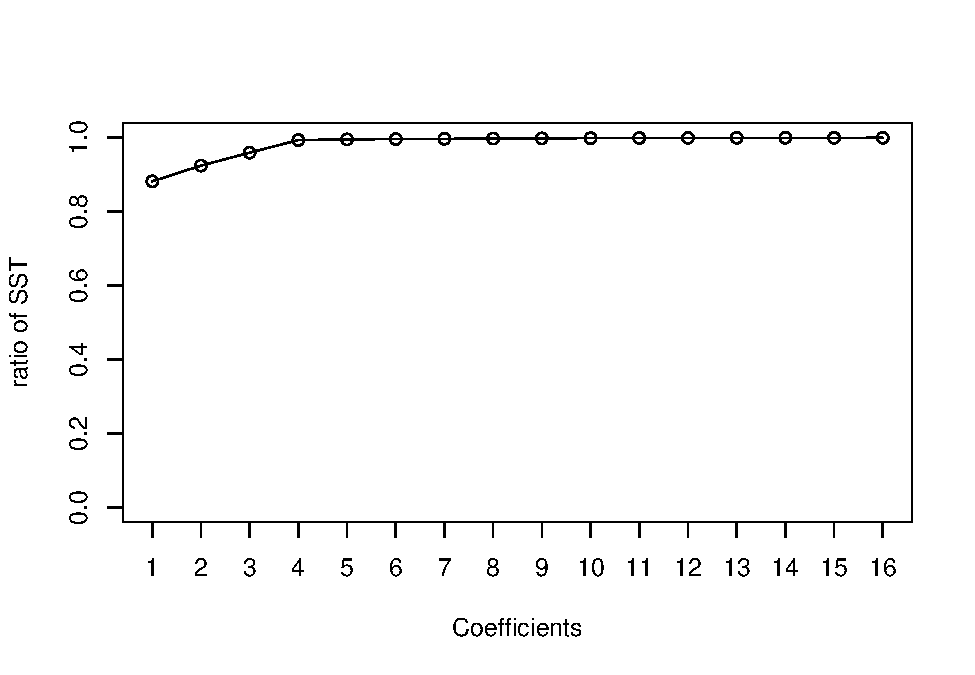
\includegraphics{12-FactorialExperiments_files/figure-latex/unnamed-chunk-4-1.pdf}

\begin{Shaded}
\begin{Highlighting}[]
\NormalTok{results[,}\DecValTok{1}\NormalTok{]}
\end{Highlighting}
\end{Shaded}

\begin{verbatim}
##  [1] "intercept"                          "moisture"                          
##  [3] "preservative:moisture"              "preservative"                      
##  [5] "moisture:acidity:temp"              "preservative:acidity"              
##  [7] "preservative:temp"                  "temp"                              
##  [9] "moisture:acidity"                   "acidity"                           
## [11] "preservative:acidity:temp"          "acidity:temp"                      
## [13] "moisture:temp"                      "preservative:moisture:acidity:temp"
## [15] "preservative:moisture:acidity"      "preservative:moisture:temp"
\end{verbatim}

\begin{Shaded}
\begin{Highlighting}[]
\NormalTok{n }\OtherTok{\textless{}{-}} \FunctionTok{length}\NormalTok{(granola}\SpecialCharTok{$}\NormalTok{response)}

\NormalTok{X }\OtherTok{\textless{}{-}} \FunctionTok{model.matrix}\NormalTok{(response}\SpecialCharTok{\textasciitilde{}}\NormalTok{moisture}\SpecialCharTok{+}\NormalTok{preservative }\SpecialCharTok{+}\NormalTok{ preservative}\SpecialCharTok{*}\NormalTok{moisture, }\AttributeTok{data =}\NormalTok{ granola)}
\NormalTok{X.r }\OtherTok{\textless{}{-}}\NormalTok{ X[,}\SpecialCharTok{{-}}\DecValTok{2}\NormalTok{]}
\NormalTok{hat.beta }\OtherTok{\textless{}{-}} \FunctionTok{solve}\NormalTok{(}\FunctionTok{t}\NormalTok{(X.r)}\SpecialCharTok{\%*\%}\NormalTok{X.r)}\SpecialCharTok{\%*\%}\FunctionTok{t}\NormalTok{(X.r)}\SpecialCharTok{\%*\%}\FunctionTok{matrix}\NormalTok{(granola}\SpecialCharTok{$}\NormalTok{response,n,}\DecValTok{1}\NormalTok{)}

\NormalTok{hat.sigma2 }\OtherTok{\textless{}{-}} \FunctionTok{sum}\NormalTok{((granola}\SpecialCharTok{$}\NormalTok{response }\SpecialCharTok{{-}}\NormalTok{ X.r }\SpecialCharTok{\%*\%}\NormalTok{hat.beta)}\SpecialCharTok{\^{}}\DecValTok{2}\NormalTok{)}\SpecialCharTok{/}\NormalTok{(n}\SpecialCharTok{{-}}\FunctionTok{ncol}\NormalTok{(X.r))}
\NormalTok{hat.sigma2}
\end{Highlighting}
\end{Shaded}

\begin{verbatim}
## [1] 3.029456
\end{verbatim}

Suppose four center-point replicates are 7.23, 7.89, 7.801, 7.39. Then, the variance estimate is the sample variance of these responses, or, \(\hat\sigma^2 = 0.101\). We may use \(\hat\sigma^2\) in t-tests of significance of the fitted regression coefficients.

\begin{Shaded}
\begin{Highlighting}[]
\FunctionTok{options}\NormalTok{(}\AttributeTok{contrasts =} \FunctionTok{c}\NormalTok{(}\StringTok{\textquotesingle{}contr.sum\textquotesingle{}}\NormalTok{, }\StringTok{\textquotesingle{}contr.sum\textquotesingle{}}\NormalTok{))}
\NormalTok{response }\OtherTok{\textless{}{-}} \FunctionTok{c}\NormalTok{(}\FloatTok{5.55}\NormalTok{,}\FloatTok{4.47}\NormalTok{,}\FloatTok{5.19}\NormalTok{,}\FloatTok{4.32}\NormalTok{,}\FloatTok{10.54}\NormalTok{,}\FloatTok{11.56}\NormalTok{,}\FloatTok{5.08}\NormalTok{,}\FloatTok{5.45}\NormalTok{,}\FloatTok{5.12}\NormalTok{,}\FloatTok{5.63}\NormalTok{,}\FloatTok{6.18}\NormalTok{,}\FloatTok{5.24}\NormalTok{,}\FloatTok{10.73}\NormalTok{,}\FloatTok{10.33}\NormalTok{,}\FloatTok{6.53}\NormalTok{,}\FloatTok{4.93}\NormalTok{)}
\NormalTok{temp }\OtherTok{\textless{}{-}} \FunctionTok{c}\NormalTok{(}\DecValTok{1}\NormalTok{,}\SpecialCharTok{{-}}\DecValTok{1}\NormalTok{,}\DecValTok{1}\NormalTok{,}\SpecialCharTok{{-}}\DecValTok{1}\NormalTok{,}\DecValTok{1}\NormalTok{,}\SpecialCharTok{{-}}\DecValTok{1}\NormalTok{,}\DecValTok{1}\NormalTok{,}\SpecialCharTok{{-}}\DecValTok{1}\NormalTok{,}\DecValTok{1}\NormalTok{,}\SpecialCharTok{{-}}\DecValTok{1}\NormalTok{,}\DecValTok{1}\NormalTok{,}\SpecialCharTok{{-}}\DecValTok{1}\NormalTok{,}\DecValTok{1}\NormalTok{,}\SpecialCharTok{{-}}\DecValTok{1}\NormalTok{,}\DecValTok{1}\NormalTok{,}\SpecialCharTok{{-}}\DecValTok{1}\NormalTok{)}
\NormalTok{preservative }\OtherTok{\textless{}{-}} \FunctionTok{c}\NormalTok{(}\DecValTok{1}\NormalTok{,}\DecValTok{1}\NormalTok{,}\SpecialCharTok{{-}}\DecValTok{1}\NormalTok{,}\SpecialCharTok{{-}}\DecValTok{1}\NormalTok{,}\DecValTok{1}\NormalTok{,}\DecValTok{1}\NormalTok{,}\SpecialCharTok{{-}}\DecValTok{1}\NormalTok{,}\SpecialCharTok{{-}}\DecValTok{1}\NormalTok{,}\DecValTok{1}\NormalTok{,}\DecValTok{1}\NormalTok{,}\SpecialCharTok{{-}}\DecValTok{1}\NormalTok{,}\SpecialCharTok{{-}}\DecValTok{1}\NormalTok{,}\DecValTok{1}\NormalTok{,}\DecValTok{1}\NormalTok{,}\SpecialCharTok{{-}}\DecValTok{1}\NormalTok{,}\SpecialCharTok{{-}}\DecValTok{1}\NormalTok{)}
\NormalTok{moisture }\OtherTok{\textless{}{-}} \FunctionTok{c}\NormalTok{(}\DecValTok{1}\NormalTok{,}\DecValTok{1}\NormalTok{,}\DecValTok{1}\NormalTok{,}\DecValTok{1}\NormalTok{,}\SpecialCharTok{{-}}\DecValTok{1}\NormalTok{,}\SpecialCharTok{{-}}\DecValTok{1}\NormalTok{,}\SpecialCharTok{{-}}\DecValTok{1}\NormalTok{,}\SpecialCharTok{{-}}\DecValTok{1}\NormalTok{,}\DecValTok{1}\NormalTok{,}\DecValTok{1}\NormalTok{,}\DecValTok{1}\NormalTok{,}\DecValTok{1}\NormalTok{,}\SpecialCharTok{{-}}\DecValTok{1}\NormalTok{,}\SpecialCharTok{{-}}\DecValTok{1}\NormalTok{,}\SpecialCharTok{{-}}\DecValTok{1}\NormalTok{,}\SpecialCharTok{{-}}\DecValTok{1}\NormalTok{)}
\NormalTok{acidity }\OtherTok{\textless{}{-}} \FunctionTok{c}\NormalTok{(}\DecValTok{1}\NormalTok{,}\DecValTok{1}\NormalTok{,}\DecValTok{1}\NormalTok{,}\DecValTok{1}\NormalTok{,}\DecValTok{1}\NormalTok{,}\DecValTok{1}\NormalTok{,}\DecValTok{1}\NormalTok{,}\DecValTok{1}\NormalTok{,}\SpecialCharTok{{-}}\DecValTok{1}\NormalTok{,}\SpecialCharTok{{-}}\DecValTok{1}\NormalTok{,}\SpecialCharTok{{-}}\DecValTok{1}\NormalTok{,}\SpecialCharTok{{-}}\DecValTok{1}\NormalTok{,}\SpecialCharTok{{-}}\DecValTok{1}\NormalTok{,}\SpecialCharTok{{-}}\DecValTok{1}\NormalTok{,}\SpecialCharTok{{-}}\DecValTok{1}\NormalTok{,}\SpecialCharTok{{-}}\DecValTok{1}\NormalTok{)}
\NormalTok{granola }\OtherTok{\textless{}{-}} \FunctionTok{data.frame}\NormalTok{(}\AttributeTok{response=}\NormalTok{response, }\AttributeTok{temp=}\FunctionTok{as.factor}\NormalTok{(temp), }\AttributeTok{preservative =} \FunctionTok{as.factor}\NormalTok{(preservative), }\AttributeTok{moisture =} \FunctionTok{as.factor}\NormalTok{(moisture), }\AttributeTok{acidity =} \FunctionTok{as.factor}\NormalTok{(acidity))}
\NormalTok{my.lm }\OtherTok{\textless{}{-}} \FunctionTok{lm}\NormalTok{(response}\SpecialCharTok{\textasciitilde{}}\NormalTok{preservative}\SpecialCharTok{*}\NormalTok{moisture}\SpecialCharTok{*}\NormalTok{acidity}\SpecialCharTok{*}\NormalTok{temp, }\AttributeTok{data =}\NormalTok{ granola)}

\FunctionTok{round}\NormalTok{(}\DecValTok{2}\SpecialCharTok{*}\NormalTok{(}\DecValTok{1}\SpecialCharTok{{-}}\FunctionTok{pt}\NormalTok{(}\FunctionTok{abs}\NormalTok{(my.lm}\SpecialCharTok{$}\NormalTok{coefficients)}\SpecialCharTok{/}\FunctionTok{sqrt}\NormalTok{(}\FloatTok{0.101}\NormalTok{),}\DecValTok{3}\NormalTok{)),}\DecValTok{4}\NormalTok{)}
\end{Highlighting}
\end{Shaded}

\begin{verbatim}
##                            (Intercept)                          preservative1 
##                                 0.0002                                 0.0257 
##                              moisture1                               acidity1 
##                                 0.0192                                 0.6530 
##                                  temp1                preservative1:moisture1 
##                                 0.5979                                 0.0247 
##                 preservative1:acidity1                     moisture1:acidity1 
##                                 0.5795                                 0.6262 
##                    preservative1:temp1                        moisture1:temp1 
##                                 0.5863                                 0.7508 
##                         acidity1:temp1       preservative1:moisture1:acidity1 
##                                 0.7375                                 0.8864 
##          preservative1:moisture1:temp1           preservative1:acidity1:temp1 
##                                 0.9121                                 0.6932 
##               moisture1:acidity1:temp1 preservative1:moisture1:acidity1:temp1 
##                                 0.4055                                 0.8412
\end{verbatim}

\hypertarget{linear-regression}{%
\chapter{Linear Regression}\label{linear-regression}}

In this chapter we study multiple linear regression under the Gauss-Markov model
\[Y = X\beta + \epsilon\]
where \(Y\) is an \(n\times 1\) vector of responses, \(X\) is and \(n\times(p+1)\) design matrix containing a leading \(n\times 1\) vector of ones (for an intercept term) and n observations on \(p\) continuous covariates (also called independent, predictor, or explanatory variables). Recall the model assumes a linear relationship between the (conditional) mean of the response and the covariates , i.e., \(E(Y|X) = X\beta\), and normal random residuals with constant variance, \(\epsilon_i \stackrel{iid}{\sim} N(0, \sigma^2)\).

Throughout this chapter we will use a large example data set to illustrate several concepts related to multiple linear regression models. The data set is the \emph{diamonds} dataframe available in the \emph{ggplot2} package in R. The data set contains prices of over 50000 diamonds, which we will predict using the size (carat) and quality (cut, color, and clarity) of the diamonds.

Among the concepts covered in this section are the following:
- Inference on the regression coefficients and conditional means (tests and CIs)
- Prediction intervals for a new response (the price of a new diamond)
- Interpretation of regression coefficients
- Choosing a model
- Diagnostics and residuals
- Dealing with outliers and influential observations

\hypertarget{diamonds-dataset}{%
\section{Diamonds dataset}\label{diamonds-dataset}}

The R package ggplot2 includes the dataframe diamonds.

\begin{Shaded}
\begin{Highlighting}[]
\FunctionTok{library}\NormalTok{(ggplot2)}
\FunctionTok{head}\NormalTok{(diamonds)}
\end{Highlighting}
\end{Shaded}

\begin{verbatim}
## # A tibble: 6 x 10
##   carat cut       color clarity depth table price     x     y     z
##   <dbl> <ord>     <ord> <ord>   <dbl> <dbl> <int> <dbl> <dbl> <dbl>
## 1  0.23 Ideal     E     SI2      61.5    55   326  3.95  3.98  2.43
## 2  0.21 Premium   E     SI1      59.8    61   326  3.89  3.84  2.31
## 3  0.23 Good      E     VS1      56.9    65   327  4.05  4.07  2.31
## 4  0.29 Premium   I     VS2      62.4    58   334  4.2   4.23  2.63
## 5  0.31 Good      J     SI2      63.3    58   335  4.34  4.35  2.75
## 6  0.24 Very Good J     VVS2     62.8    57   336  3.94  3.96  2.48
\end{verbatim}

\begin{Shaded}
\begin{Highlighting}[]
\FunctionTok{levels}\NormalTok{(diamonds}\SpecialCharTok{$}\NormalTok{cut)}
\end{Highlighting}
\end{Shaded}

\begin{verbatim}
## [1] "Fair"      "Good"      "Very Good" "Premium"   "Ideal"
\end{verbatim}

\begin{Shaded}
\begin{Highlighting}[]
\FunctionTok{levels}\NormalTok{(diamonds}\SpecialCharTok{$}\NormalTok{clarity)}
\end{Highlighting}
\end{Shaded}

\begin{verbatim}
## [1] "I1"   "SI2"  "SI1"  "VS2"  "VS1"  "VVS2" "VVS1" "IF"
\end{verbatim}

\begin{Shaded}
\begin{Highlighting}[]
\FunctionTok{levels}\NormalTok{(diamonds}\SpecialCharTok{$}\NormalTok{color)}
\end{Highlighting}
\end{Shaded}

\begin{verbatim}
## [1] "D" "E" "F" "G" "H" "I" "J"
\end{verbatim}

Cut, color, and clarity are coded as ordinal categorical variables. It may be helpful to use numeric versions of these; for example, cut cut.num coded as an integer 1, 2, 3, 4, or 5, rather than an ordinal variable.

\begin{Shaded}
\begin{Highlighting}[]
\NormalTok{diamonds}\SpecialCharTok{$}\NormalTok{color.num }\OtherTok{\textless{}{-}} \FunctionTok{as.numeric}\NormalTok{(diamonds}\SpecialCharTok{$}\NormalTok{color)}
\NormalTok{diamonds}\SpecialCharTok{$}\NormalTok{cut.num }\OtherTok{\textless{}{-}} \FunctionTok{as.numeric}\NormalTok{(diamonds}\SpecialCharTok{$}\NormalTok{cut)}
\NormalTok{diamonds}\SpecialCharTok{$}\NormalTok{clarity.num }\OtherTok{\textless{}{-}} \FunctionTok{as.numeric}\NormalTok{(diamonds}\SpecialCharTok{$}\NormalTok{clarity)}
\end{Highlighting}
\end{Shaded}

The model we build may depend on what purpose it is to be used for.
- Inference: models built to be interpretable and offer best explanation of response in terms of explanatory variables
- Prediction: models built to predict the response given explanatory variables
Models built for inference tend to be simpler/include fewer variables than models built for prediction. For example, a model built for inference may exclude explanatory variables exhibiting collinearity, because collinearity makes the model more difficult to interpret, but collinearity generally does not make the model worse at prediction.\\
First we will build a model for inference. Since we are interested in hypothesis testing as part of inference, we will check all the model assumptions. These are less important for prediction.

\hypertarget{checking-linearity}{%
\section{Checking Linearity}\label{checking-linearity}}

Our multiple linear regression model assumes the conditional mean of response (price) given explanatory variables(carat, cut, color, clarity) is a linear function of those variables. For a given model we can check linearity by examining residuals versus predicted values; there should be no pattern in that plot. We can also do a preliminary check by plotting the response versus each explanatory variable (so long as there are not too many) to see whether any variables exhibit a nonlinear relationship with response. If price is non-linear in a variable, then we can use a transformation to make the relationship more linear.

The square root transformation on price works best in the plot of carat versus price.

\begin{Shaded}
\begin{Highlighting}[]
\FunctionTok{plot}\NormalTok{(diamonds}\SpecialCharTok{$}\NormalTok{carat, diamonds}\SpecialCharTok{$}\NormalTok{price)}
\end{Highlighting}
\end{Shaded}

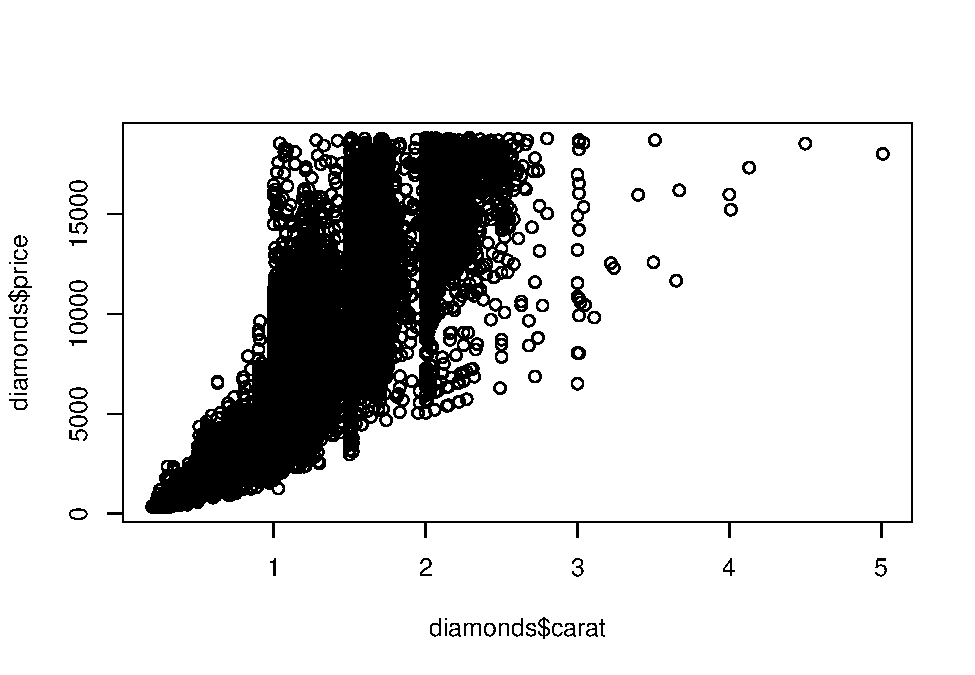
\includegraphics{13-MultipleLinearRegression_files/figure-latex/unnamed-chunk-3-1.pdf}

\begin{Shaded}
\begin{Highlighting}[]
\FunctionTok{plot}\NormalTok{(diamonds}\SpecialCharTok{$}\NormalTok{carat, }\FunctionTok{log}\NormalTok{(diamonds}\SpecialCharTok{$}\NormalTok{price))}
\end{Highlighting}
\end{Shaded}

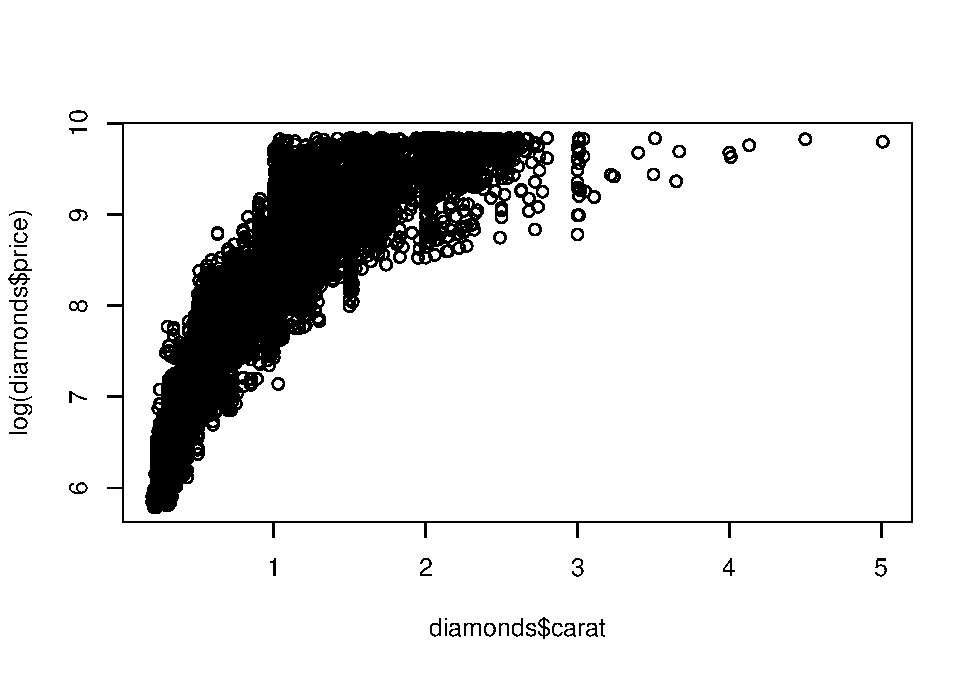
\includegraphics{13-MultipleLinearRegression_files/figure-latex/unnamed-chunk-3-2.pdf}

\begin{Shaded}
\begin{Highlighting}[]
\FunctionTok{plot}\NormalTok{(diamonds}\SpecialCharTok{$}\NormalTok{carat, }\FunctionTok{sqrt}\NormalTok{(diamonds}\SpecialCharTok{$}\NormalTok{price))}
\end{Highlighting}
\end{Shaded}

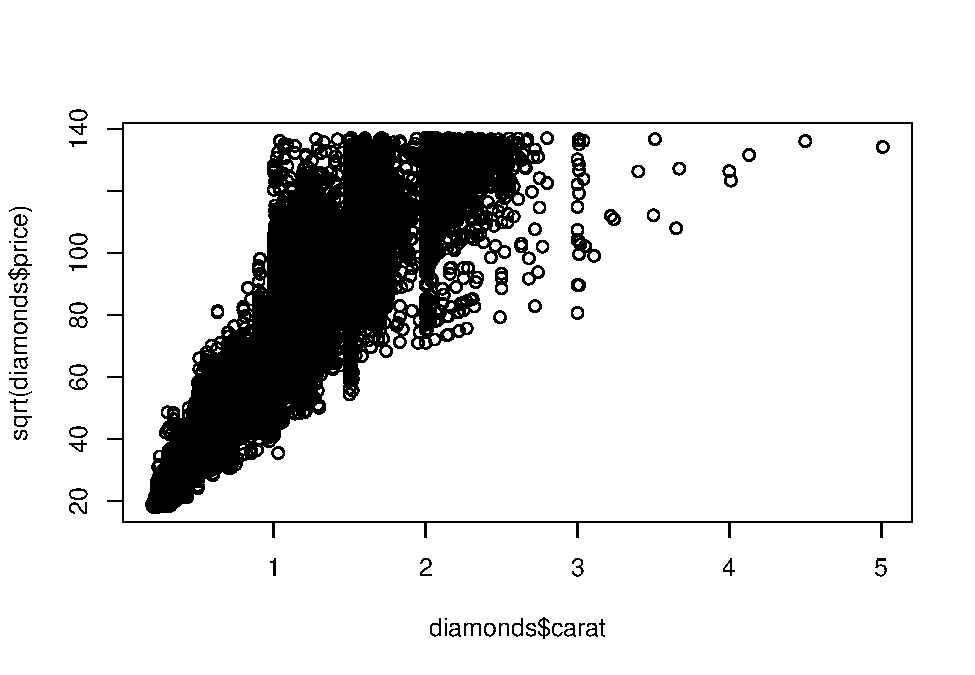
\includegraphics{13-MultipleLinearRegression_files/figure-latex/unnamed-chunk-3-3.pdf}

\begin{Shaded}
\begin{Highlighting}[]
\FunctionTok{boxplot}\NormalTok{(diamonds}\SpecialCharTok{$}\NormalTok{price}\SpecialCharTok{\textasciitilde{}}\NormalTok{diamonds}\SpecialCharTok{$}\NormalTok{cut)}
\end{Highlighting}
\end{Shaded}

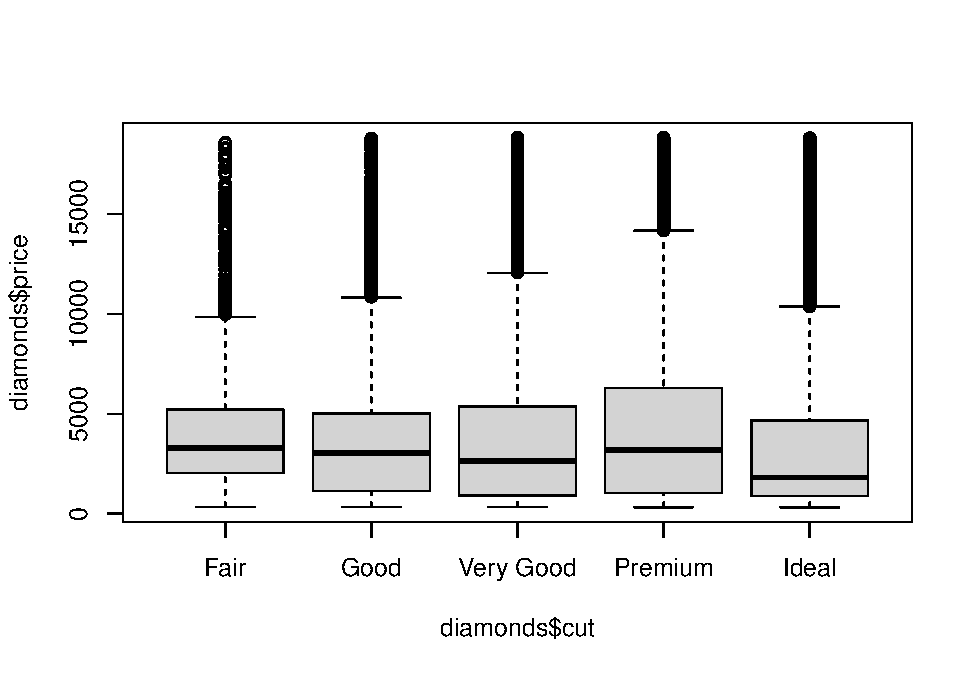
\includegraphics{13-MultipleLinearRegression_files/figure-latex/unnamed-chunk-3-4.pdf}

\begin{Shaded}
\begin{Highlighting}[]
\FunctionTok{boxplot}\NormalTok{(diamonds}\SpecialCharTok{$}\NormalTok{price}\SpecialCharTok{\textasciitilde{}}\NormalTok{diamonds}\SpecialCharTok{$}\NormalTok{clarity)}
\end{Highlighting}
\end{Shaded}

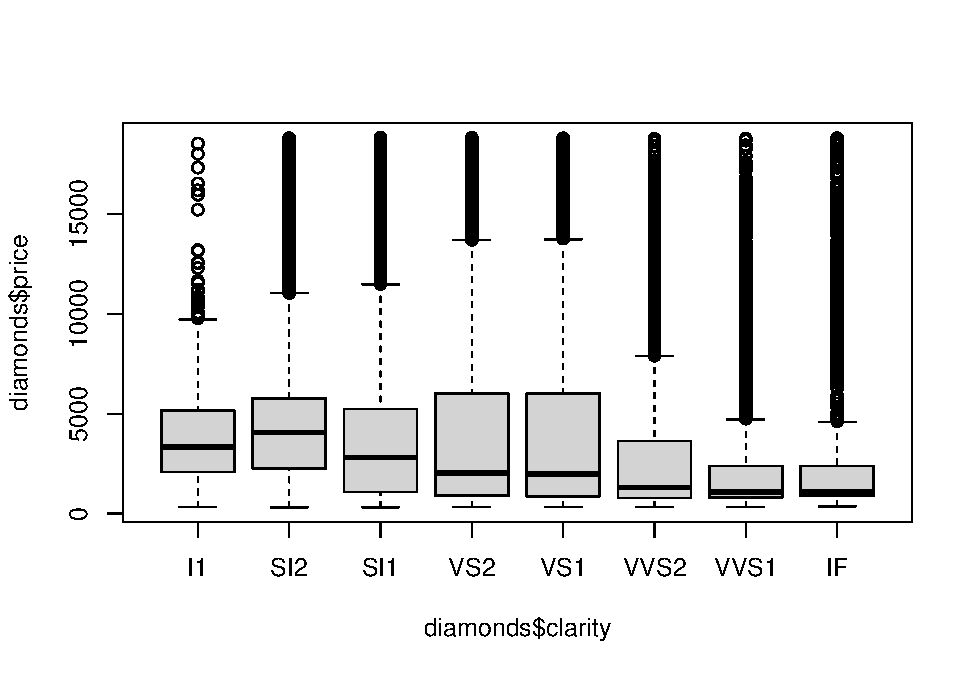
\includegraphics{13-MultipleLinearRegression_files/figure-latex/unnamed-chunk-3-5.pdf}

\begin{Shaded}
\begin{Highlighting}[]
\FunctionTok{boxplot}\NormalTok{(diamonds}\SpecialCharTok{$}\NormalTok{price}\SpecialCharTok{\textasciitilde{}}\NormalTok{diamonds}\SpecialCharTok{$}\NormalTok{color)}
\end{Highlighting}
\end{Shaded}

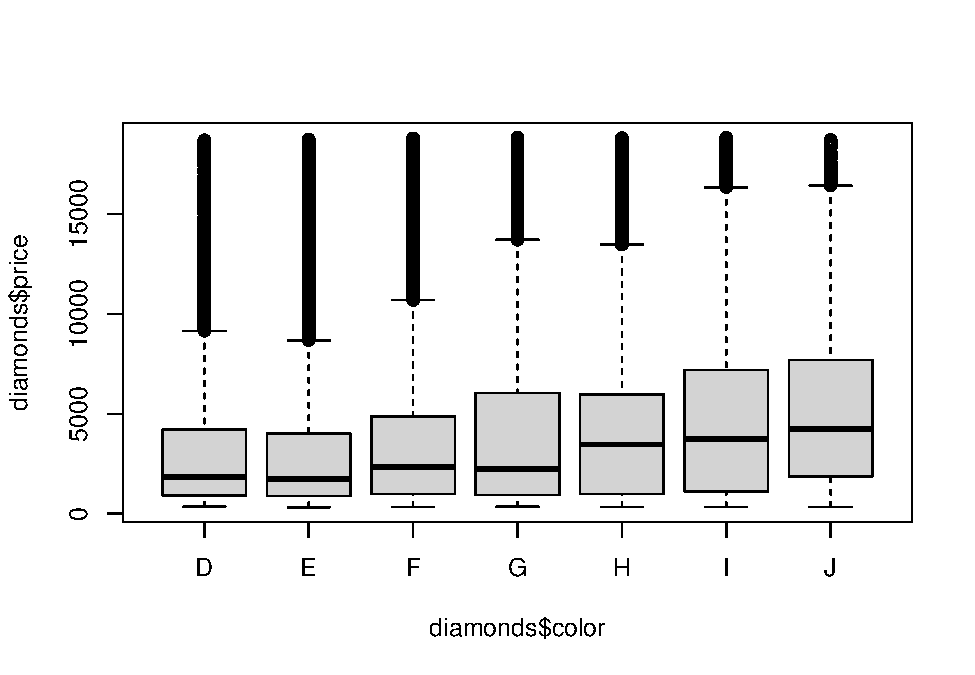
\includegraphics{13-MultipleLinearRegression_files/figure-latex/unnamed-chunk-3-6.pdf}

Note that if we fit a model in R with the ordinal-factor versions of the diamond quality variables R uses as many orthogonal polynomial contrasts as it can for each ordinal factor.

\begin{Shaded}
\begin{Highlighting}[]
\NormalTok{full.lm.sqrt }\OtherTok{\textless{}{-}} \FunctionTok{lm}\NormalTok{(}\FunctionTok{sqrt}\NormalTok{(price)}\SpecialCharTok{\textasciitilde{}}\NormalTok{carat}\SpecialCharTok{+}\NormalTok{cut}\SpecialCharTok{+}\NormalTok{color}\SpecialCharTok{+}\NormalTok{clarity, }\AttributeTok{data =}\NormalTok{ diamonds)}
\FunctionTok{plot}\NormalTok{(full.lm.sqrt}\SpecialCharTok{$}\NormalTok{fitted.values,full.lm.sqrt}\SpecialCharTok{$}\NormalTok{residuals) }
\end{Highlighting}
\end{Shaded}

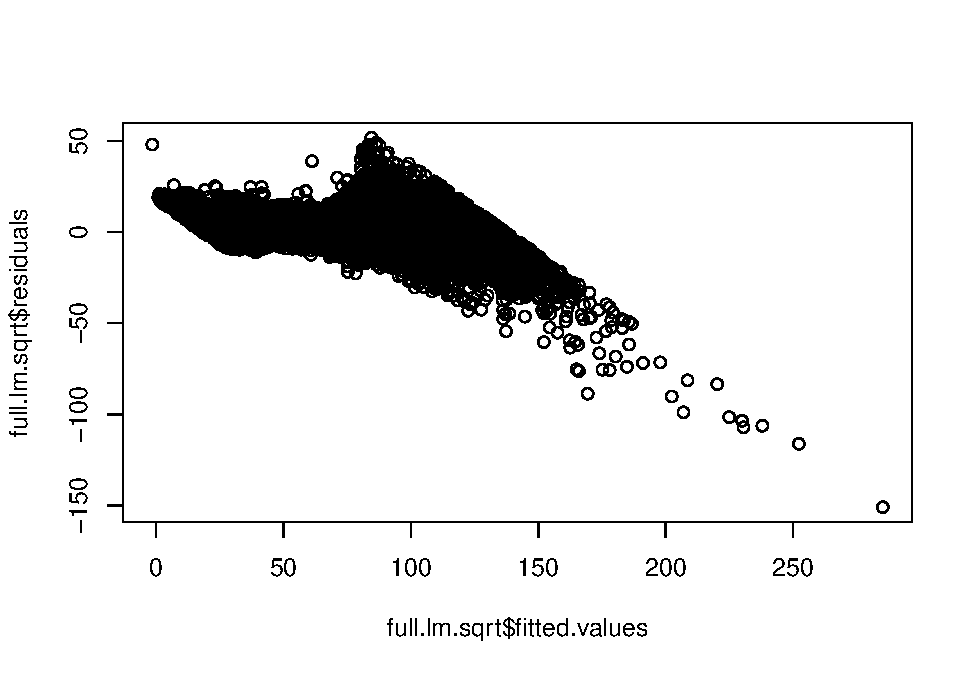
\includegraphics{13-MultipleLinearRegression_files/figure-latex/unnamed-chunk-4-1.pdf}

\begin{Shaded}
\begin{Highlighting}[]
\FunctionTok{summary}\NormalTok{(full.lm.sqrt)}
\end{Highlighting}
\end{Shaded}

\begin{verbatim}
## 
## Call:
## lm(formula = sqrt(price) ~ carat + cut + color + clarity, data = diamonds)
## 
## Residuals:
##      Min       1Q   Median       3Q      Max 
## -150.936   -3.296   -0.478    2.824   51.690 
## 
## Coefficients:
##              Estimate Std. Error  t value Pr(>|t|)    
## (Intercept)   0.56869    0.07737    7.351 2.00e-13 ***
## carat        64.55472    0.06659  969.371  < 2e-16 ***
## cut.L         3.50254    0.11253   31.124  < 2e-16 ***
## cut.Q        -1.69032    0.09912  -17.054  < 2e-16 ***
## cut.C         1.10438    0.08609   12.828  < 2e-16 ***
## cut^4         0.02937    0.06894    0.426    0.670    
## color.L     -13.98189    0.09802 -142.646  < 2e-16 ***
## color.Q      -4.61348    0.08921  -51.712  < 2e-16 ***
## color.C      -0.79061    0.08340   -9.480  < 2e-16 ***
## color^4       0.67221    0.07659    8.777  < 2e-16 ***
## color^5      -0.54516    0.07236   -7.533 5.02e-14 ***
## color^6      -0.09971    0.06579   -1.516    0.130    
## clarity.L    26.37314    0.17062  154.572  < 2e-16 ***
## clarity.Q   -12.45929    0.15953  -78.100  < 2e-16 ***
## clarity.C     6.50359    0.13658   47.619  < 2e-16 ***
## clarity^4    -2.37701    0.10924  -21.761  < 2e-16 ***
## clarity^5     1.60112    0.08915   17.960  < 2e-16 ***
## clarity^6     0.05858    0.07768    0.754    0.451    
## clarity^7     0.49801    0.06853    7.267 3.72e-13 ***
## ---
## Signif. codes:  0 '***' 0.001 '**' 0.01 '*' 0.05 '.' 0.1 ' ' 1
## 
## Residual standard error: 6.402 on 53921 degrees of freedom
## Multiple R-squared:  0.9501, Adjusted R-squared:   0.95 
## F-statistic: 5.7e+04 on 18 and 53921 DF,  p-value: < 2.2e-16
\end{verbatim}

\begin{Shaded}
\begin{Highlighting}[]
\FunctionTok{AIC}\NormalTok{(full.lm.sqrt)}
\end{Highlighting}
\end{Shaded}

\begin{verbatim}
## [1] 353387.4
\end{verbatim}

\begin{Shaded}
\begin{Highlighting}[]
\FunctionTok{BIC}\NormalTok{(full.lm.sqrt)}
\end{Highlighting}
\end{Shaded}

\begin{verbatim}
## [1] 353565.3
\end{verbatim}

A simpler model re-codes the ordinal factors as integers. This model is equivalent to the above model with only linear contrasts for each factor, hence the large difference in number of parameters.

\begin{Shaded}
\begin{Highlighting}[]
\NormalTok{full.lm.sqrt }\OtherTok{\textless{}{-}} \FunctionTok{lm}\NormalTok{(}\FunctionTok{sqrt}\NormalTok{(price)}\SpecialCharTok{\textasciitilde{}}\NormalTok{carat}\SpecialCharTok{+}\NormalTok{cut.num}\SpecialCharTok{+}\NormalTok{color.num}\SpecialCharTok{+}\NormalTok{clarity.num, }\AttributeTok{data =}\NormalTok{ diamonds)}
\FunctionTok{plot}\NormalTok{(full.lm.sqrt}\SpecialCharTok{$}\NormalTok{fitted.values,full.lm.sqrt}\SpecialCharTok{$}\NormalTok{residuals) }
\end{Highlighting}
\end{Shaded}

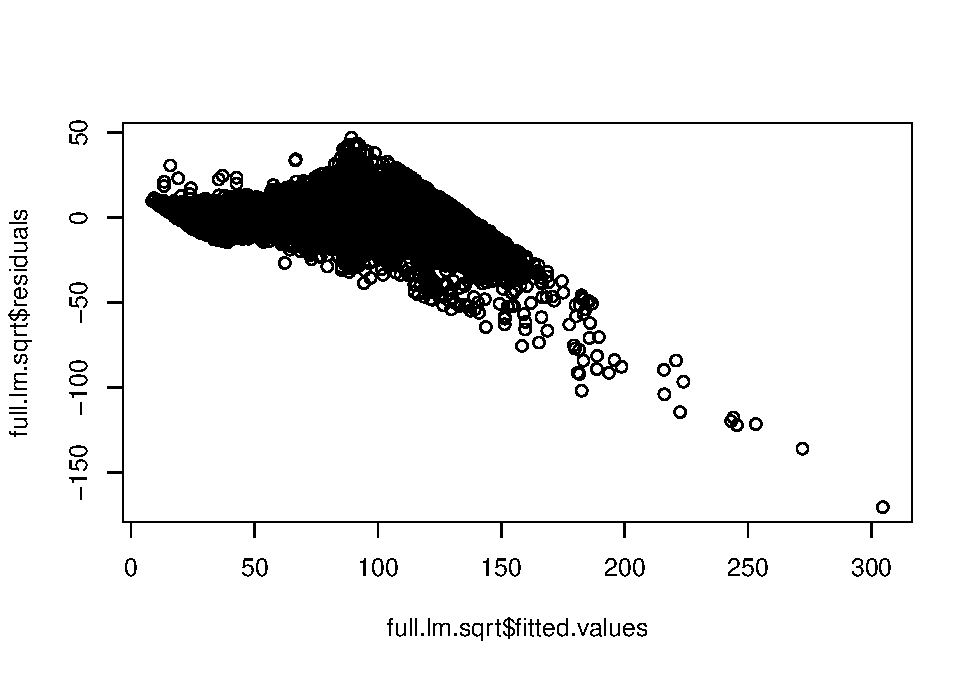
\includegraphics{13-MultipleLinearRegression_files/figure-latex/unnamed-chunk-5-1.pdf}

\begin{Shaded}
\begin{Highlighting}[]
\FunctionTok{summary}\NormalTok{(full.lm.sqrt)}
\end{Highlighting}
\end{Shaded}

\begin{verbatim}
## 
## Call:
## lm(formula = sqrt(price) ~ carat + cut.num + color.num + clarity.num, 
##     data = diamonds)
## 
## Residuals:
##      Min       1Q   Median       3Q      Max 
## -170.349   -3.303   -0.046    3.146   46.910 
## 
## Coefficients:
##             Estimate Std. Error t value Pr(>|t|)    
## (Intercept) -2.80669    0.15774  -17.79   <2e-16 ***
## carat       63.83681    0.07256  879.73   <2e-16 ***
## cut.num      0.79943    0.02781   28.75   <2e-16 ***
## color.num   -2.34832    0.01888 -124.38   <2e-16 ***
## clarity.num  3.20315    0.02017  158.84   <2e-16 ***
## ---
## Signif. codes:  0 '***' 0.001 '**' 0.01 '*' 0.05 '.' 0.1 ' ' 1
## 
## Residual standard error: 7.061 on 53935 degrees of freedom
## Multiple R-squared:  0.9392, Adjusted R-squared:  0.9392 
## F-statistic: 2.084e+05 on 4 and 53935 DF,  p-value: < 2.2e-16
\end{verbatim}

\begin{Shaded}
\begin{Highlighting}[]
\FunctionTok{AIC}\NormalTok{(full.lm.sqrt)}
\end{Highlighting}
\end{Shaded}

\begin{verbatim}
## [1] 363946.8
\end{verbatim}

\begin{Shaded}
\begin{Highlighting}[]
\FunctionTok{BIC}\NormalTok{(full.lm.sqrt)}
\end{Highlighting}
\end{Shaded}

\begin{verbatim}
## [1] 364000.1
\end{verbatim}

Our residuals have a pattern. We may be able to use ``interactions'' to obtain a better-fitting model due to \emph{multicollinearity}---another term for correlation between covariates.

\hypertarget{multicollinearity}{%
\section{Multicollinearity}\label{multicollinearity}}

We see that diamonds of the worst cuts, colors, and clarities are also the largest diamonds on average. That makes sense. These diamonds are not worth much of anything unless they are large; the small diamonds of poor quality didn't even make it to the market for diamonds. There is weak multicollinearity that probably is not enough to harm the interpretability of the model if all variables are included.

\begin{Shaded}
\begin{Highlighting}[]
\FunctionTok{boxplot}\NormalTok{(diamonds}\SpecialCharTok{$}\NormalTok{carat}\SpecialCharTok{\textasciitilde{}}\NormalTok{diamonds}\SpecialCharTok{$}\NormalTok{cut)}
\end{Highlighting}
\end{Shaded}

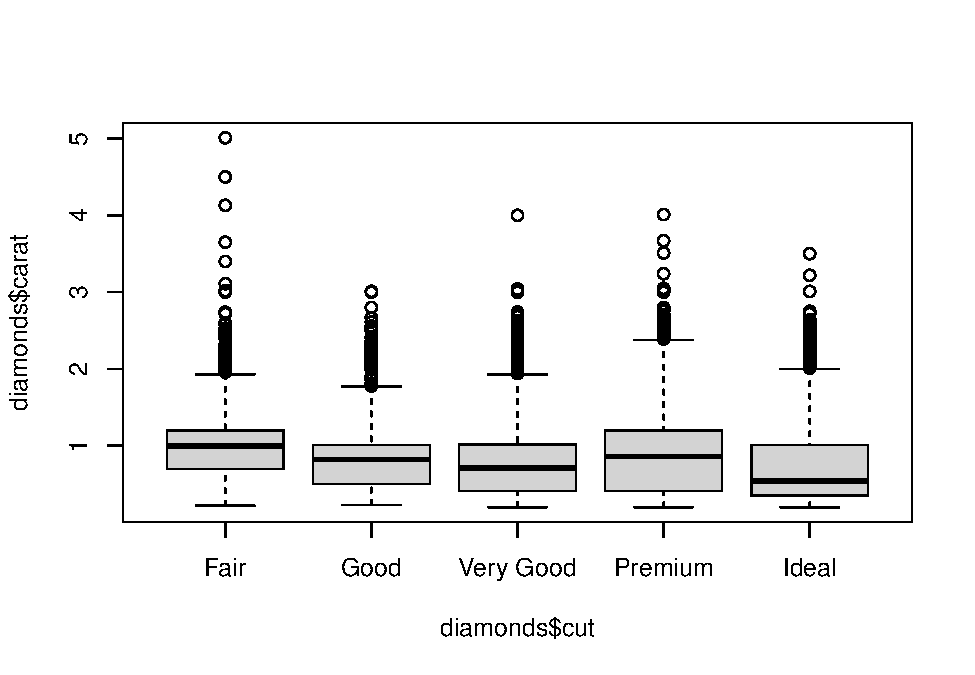
\includegraphics{13-MultipleLinearRegression_files/figure-latex/unnamed-chunk-6-1.pdf}

\begin{Shaded}
\begin{Highlighting}[]
\FunctionTok{boxplot}\NormalTok{(diamonds}\SpecialCharTok{$}\NormalTok{carat}\SpecialCharTok{\textasciitilde{}}\NormalTok{diamonds}\SpecialCharTok{$}\NormalTok{clarity)}
\end{Highlighting}
\end{Shaded}

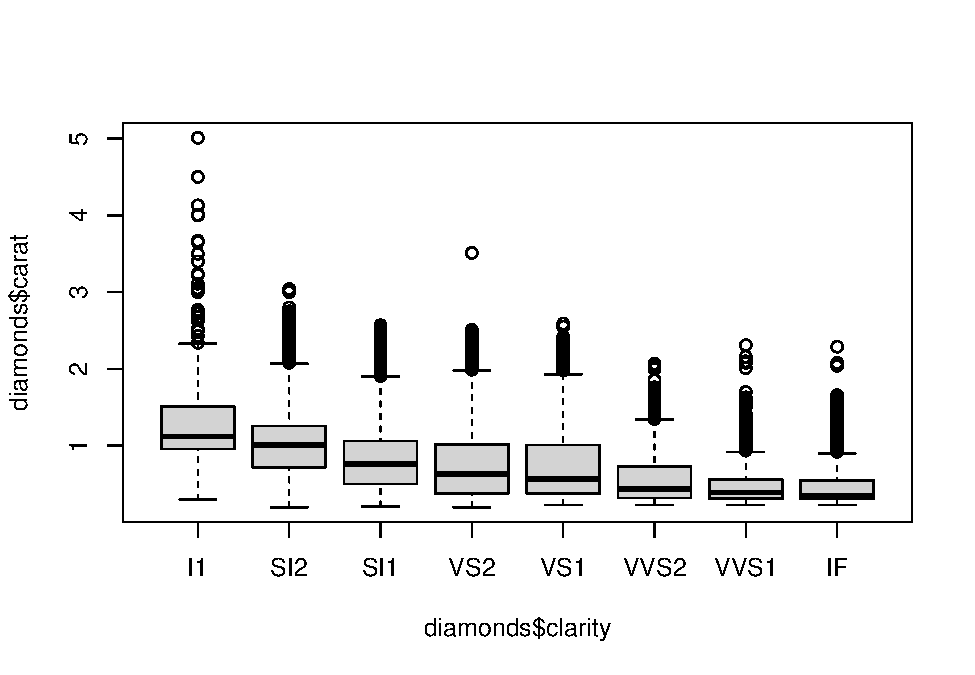
\includegraphics{13-MultipleLinearRegression_files/figure-latex/unnamed-chunk-6-2.pdf}

\begin{Shaded}
\begin{Highlighting}[]
\FunctionTok{boxplot}\NormalTok{(diamonds}\SpecialCharTok{$}\NormalTok{carat}\SpecialCharTok{\textasciitilde{}}\NormalTok{diamonds}\SpecialCharTok{$}\NormalTok{color)}
\end{Highlighting}
\end{Shaded}

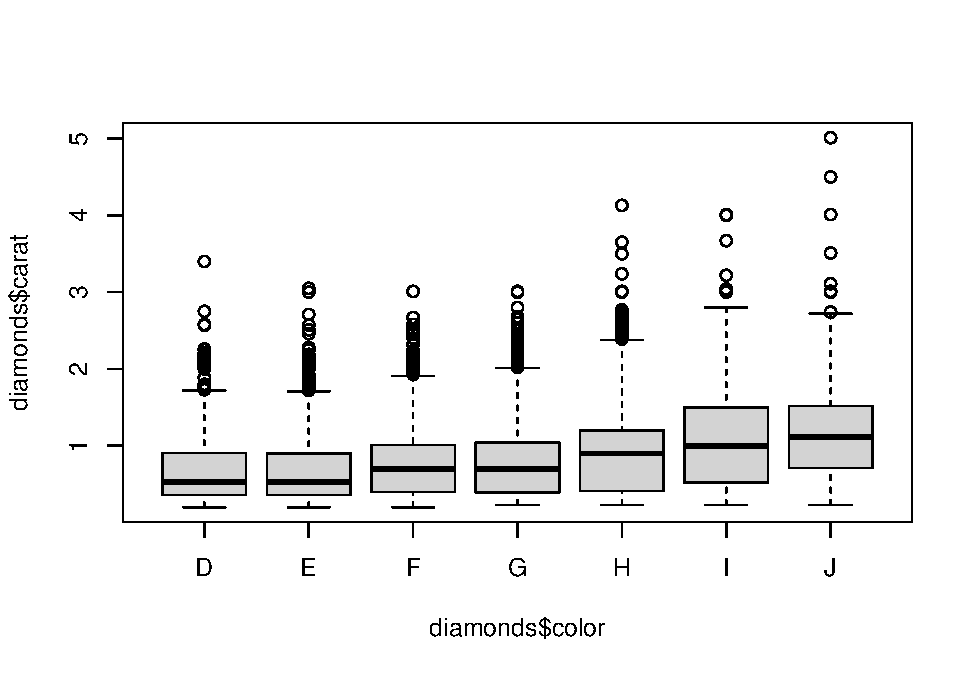
\includegraphics{13-MultipleLinearRegression_files/figure-latex/unnamed-chunk-6-3.pdf}

\begin{Shaded}
\begin{Highlighting}[]
\FunctionTok{cor}\NormalTok{(diamonds}\SpecialCharTok{$}\NormalTok{carat,}\FunctionTok{as.numeric}\NormalTok{(diamonds}\SpecialCharTok{$}\NormalTok{cut))}
\end{Highlighting}
\end{Shaded}

\begin{verbatim}
## [1] -0.134967
\end{verbatim}

\begin{Shaded}
\begin{Highlighting}[]
\FunctionTok{cor}\NormalTok{(diamonds}\SpecialCharTok{$}\NormalTok{carat,}\FunctionTok{as.numeric}\NormalTok{(diamonds}\SpecialCharTok{$}\NormalTok{clarity))}
\end{Highlighting}
\end{Shaded}

\begin{verbatim}
## [1] -0.3528406
\end{verbatim}

\begin{Shaded}
\begin{Highlighting}[]
\FunctionTok{cor}\NormalTok{(diamonds}\SpecialCharTok{$}\NormalTok{carat,}\FunctionTok{as.numeric}\NormalTok{(diamonds}\SpecialCharTok{$}\NormalTok{color))}
\end{Highlighting}
\end{Shaded}

\begin{verbatim}
## [1] 0.2914368
\end{verbatim}

\hypertarget{model-with-carat-interactions}{%
\section{Model with carat interactions}\label{model-with-carat-interactions}}

Including the carat interaction with cut, color, and clarity substantially improves the fit of the model as measured by \(R^2\) and \(R^2_{adj}\), the residual error/variance, and as evidenced by the residual vs predicted plot.

\begin{Shaded}
\begin{Highlighting}[]
\NormalTok{full.lm.sqrt }\OtherTok{\textless{}{-}} \FunctionTok{lm}\NormalTok{(}\FunctionTok{sqrt}\NormalTok{(price)}\SpecialCharTok{\textasciitilde{}}\NormalTok{carat}\SpecialCharTok{+}\NormalTok{cut.num}\SpecialCharTok{+}\NormalTok{color.num}\SpecialCharTok{+}\NormalTok{clarity.num }\SpecialCharTok{+}\NormalTok{ carat}\SpecialCharTok{*}\NormalTok{clarity.num }\SpecialCharTok{+}\NormalTok{ carat}\SpecialCharTok{*}\NormalTok{color.num }\SpecialCharTok{+}\NormalTok{carat}\SpecialCharTok{*}\NormalTok{cut.num, }\AttributeTok{data =}\NormalTok{ diamonds)}
\FunctionTok{summary}\NormalTok{(full.lm.sqrt)}
\end{Highlighting}
\end{Shaded}

\begin{verbatim}
## 
## Call:
## lm(formula = sqrt(price) ~ carat + cut.num + color.num + clarity.num + 
##     carat * clarity.num + carat * color.num + carat * cut.num, 
##     data = diamonds)
## 
## Residuals:
##     Min      1Q  Median      3Q     Max 
## -77.115  -2.174  -0.087   2.314  34.034 
## 
## Coefficients:
##                   Estimate Std. Error t value Pr(>|t|)    
## (Intercept)        5.35572    0.19406   27.60  < 2e-16 ***
## carat             52.84947    0.20639  256.06  < 2e-16 ***
## cut.num           -0.23567    0.03783   -6.23 4.71e-10 ***
## color.num          0.45156    0.02413   18.71  < 2e-16 ***
## clarity.num       -0.69980    0.02430  -28.80  < 2e-16 ***
## carat:clarity.num  5.63633    0.02855  197.40  < 2e-16 ***
## carat:color.num   -3.39270    0.02518 -134.74  < 2e-16 ***
## carat:cut.num      1.39771    0.03972   35.19  < 2e-16 ***
## ---
## Signif. codes:  0 '***' 0.001 '**' 0.01 '*' 0.05 '.' 0.1 ' ' 1
## 
## Residual standard error: 4.771 on 53932 degrees of freedom
## Multiple R-squared:  0.9723, Adjusted R-squared:  0.9723 
## F-statistic: 2.701e+05 on 7 and 53932 DF,  p-value: < 2.2e-16
\end{verbatim}

\begin{Shaded}
\begin{Highlighting}[]
\FunctionTok{AIC}\NormalTok{(full.lm.sqrt)}
\end{Highlighting}
\end{Shaded}

\begin{verbatim}
## [1] 321649.3
\end{verbatim}

\begin{Shaded}
\begin{Highlighting}[]
\FunctionTok{BIC}\NormalTok{(full.lm.sqrt)}
\end{Highlighting}
\end{Shaded}

\begin{verbatim}
## [1] 321729.4
\end{verbatim}

\begin{Shaded}
\begin{Highlighting}[]
\FunctionTok{qqnorm}\NormalTok{(full.lm.sqrt}\SpecialCharTok{$}\NormalTok{residuals)}
\FunctionTok{qqline}\NormalTok{(full.lm.sqrt}\SpecialCharTok{$}\NormalTok{residuals)}
\end{Highlighting}
\end{Shaded}

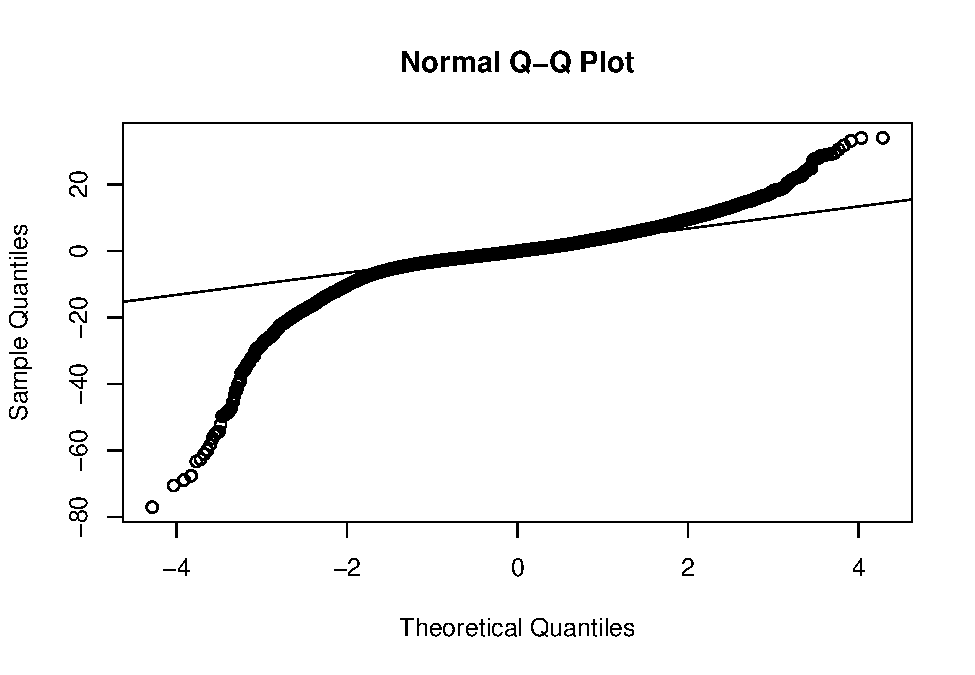
\includegraphics{13-MultipleLinearRegression_files/figure-latex/unnamed-chunk-7-1.pdf}

\begin{Shaded}
\begin{Highlighting}[]
\FunctionTok{plot}\NormalTok{(full.lm.sqrt}\SpecialCharTok{$}\NormalTok{fitted.values,full.lm.sqrt}\SpecialCharTok{$}\NormalTok{residuals) }
\end{Highlighting}
\end{Shaded}

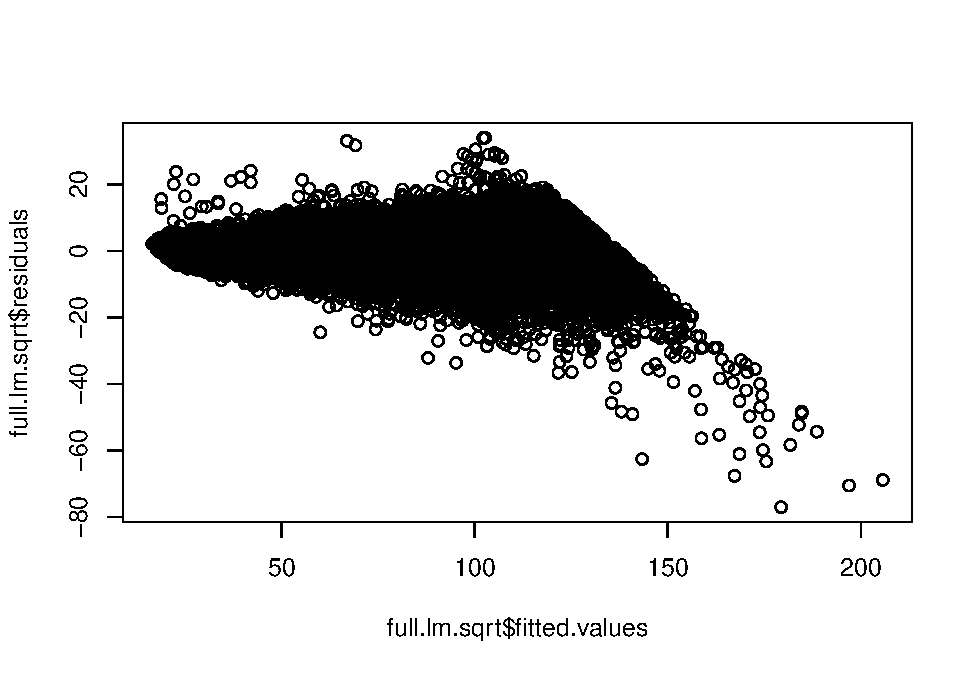
\includegraphics{13-MultipleLinearRegression_files/figure-latex/unnamed-chunk-7-2.pdf}

\begin{Shaded}
\begin{Highlighting}[]
\FunctionTok{plot}\NormalTok{(diamonds}\SpecialCharTok{$}\NormalTok{carat,full.lm.sqrt}\SpecialCharTok{$}\NormalTok{residuals) }
\end{Highlighting}
\end{Shaded}

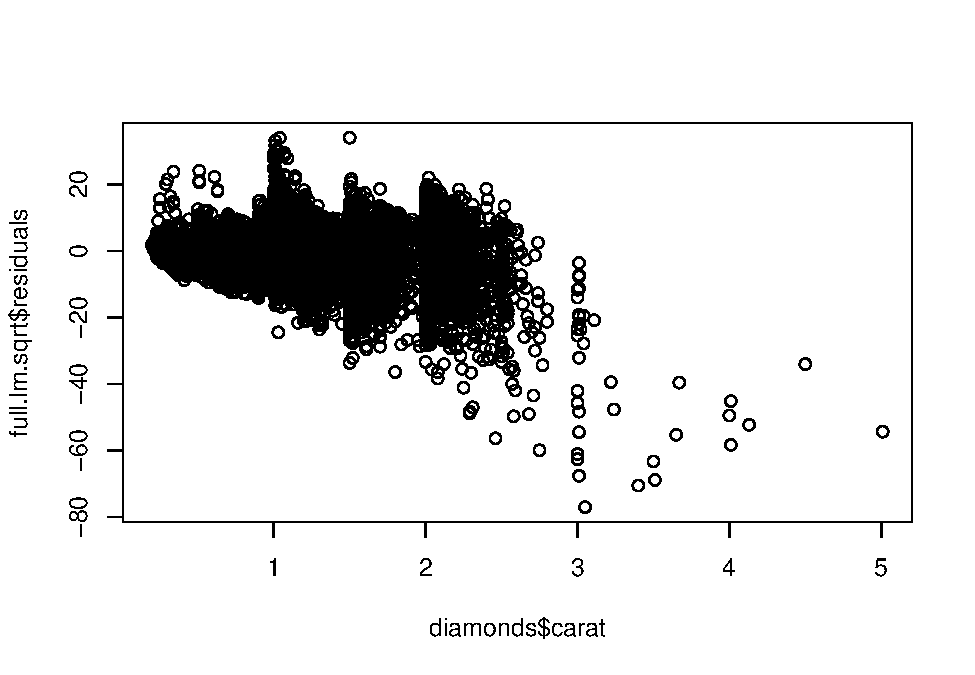
\includegraphics{13-MultipleLinearRegression_files/figure-latex/unnamed-chunk-7-3.pdf}

\hypertarget{interpreting-the-model}{%
\section{Interpreting the model}\label{interpreting-the-model}}

What about interpretability? We need to be specific about our interpretations, but the (simple) interactions model is certainly interpretable. For example, the first diamond in the data has carat 0.23, it is cut, color, and clarity levels 5, 2, and 2. The interpretation of the fitted betas is as follows, if we hold cut, color, and clarity constant, and increase carat by , say, 0.05, then we will increase sqrt(price) by \(3.216264 = 0.05*(52.84947 + 5*1.39771 -2*3.39270+2*5.63633)\). For another example, suppose if that diamond were cut level 4 instead of 5? Then, it's sqrt(price) would change by \(-0.0858033 = 0.23567 - 0.23*1.39771\).

\begin{Shaded}
\begin{Highlighting}[]
\FunctionTok{as.matrix}\NormalTok{(}\FunctionTok{head}\NormalTok{(diamonds))[}\DecValTok{1}\NormalTok{,]}
\end{Highlighting}
\end{Shaded}

\begin{verbatim}
##       carat         cut       color     clarity       depth       table 
##      "0.23"     "Ideal"         "E"       "SI2"      "61.5"        "55" 
##       price           x           y           z   color.num     cut.num 
##       "326"      "3.95"      "3.98"      "2.43"         "2"         "5" 
## clarity.num 
##         "2"
\end{verbatim}

\begin{Shaded}
\begin{Highlighting}[]
\NormalTok{full.lm.sqrt}\SpecialCharTok{$}\NormalTok{fitted.values[}\DecValTok{1}\NormalTok{]}
\end{Highlighting}
\end{Shaded}

\begin{verbatim}
##        1 
## 18.47571
\end{verbatim}

\begin{Shaded}
\begin{Highlighting}[]
\NormalTok{X}\OtherTok{\textless{}{-}} \FunctionTok{model.matrix}\NormalTok{(}\FunctionTok{sqrt}\NormalTok{(price)}\SpecialCharTok{\textasciitilde{}}\NormalTok{carat}\SpecialCharTok{+}\NormalTok{cut.num}\SpecialCharTok{+}\NormalTok{color.num}\SpecialCharTok{+}\NormalTok{clarity.num }\SpecialCharTok{+}\NormalTok{ carat}\SpecialCharTok{*}\NormalTok{clarity.num }\SpecialCharTok{+}\NormalTok{ carat}\SpecialCharTok{*}\NormalTok{color.num }\SpecialCharTok{+}\NormalTok{carat}\SpecialCharTok{*}\NormalTok{cut.num, }\AttributeTok{data =}\NormalTok{ diamonds)}
\NormalTok{X[}\DecValTok{1}\NormalTok{,]}
\end{Highlighting}
\end{Shaded}

\begin{verbatim}
##       (Intercept)             carat           cut.num         color.num 
##              1.00              0.23              5.00              2.00 
##       clarity.num carat:clarity.num   carat:color.num     carat:cut.num 
##              2.00              0.46              0.46              1.15
\end{verbatim}

\hypertarget{checking-constant-variance}{%
\section{Checking Constant Variance}\label{checking-constant-variance}}

As you may have noticed, the observed residuals ``fan out''; they increase in magnitude with the value of the predicted sqrt(price). What does this mean for our model/inferences? One consequence is that our tests/CIs for conditional means may not be valid in terms of their nominal \(\alpha\) Type 1 error/coverage probability for explanatory variable values with a large estimated mean sqrt(price) value. The variance of the fitted conditional mean \(\hat\mu_{Y|x} = x^{\top}\hat\beta\) is larger than estimated by \(MSEx^\top(X^\top X)^{-1}x\) for large values of \(x^{\top}\hat\beta\). The reason is that the variance of \(\epsilon_i\) seems to be \(\sigma^2 \times\text{carat}\) rather than \(\sigma^2\).

We will come back to this topic later to study what can be done about non-constant variance.

\hypertarget{normality}{%
\section{Normality}\label{normality}}

How bad is this? The residuals are ``normal'' for about the middle 90-95 \% of their distribution. There are some very extreme residuals; these are diamonds with prices poorly predicted by the model. We should be cautious when interpreting the model for these diamonds. We have likely missed some important information about their prices.

\begin{Shaded}
\begin{Highlighting}[]
\FunctionTok{qqnorm}\NormalTok{(full.lm.sqrt}\SpecialCharTok{$}\NormalTok{residuals}\SpecialCharTok{/}\FunctionTok{sd}\NormalTok{(full.lm.sqrt}\SpecialCharTok{$}\NormalTok{residuals))}
\FunctionTok{qqline}\NormalTok{(full.lm.sqrt}\SpecialCharTok{$}\NormalTok{residuals}\SpecialCharTok{/}\FunctionTok{sd}\NormalTok{(full.lm.sqrt}\SpecialCharTok{$}\NormalTok{residuals), }\AttributeTok{probs =} \FunctionTok{c}\NormalTok{(}\FloatTok{0.05}\NormalTok{, }\FloatTok{0.95}\NormalTok{))}

\NormalTok{sorted }\OtherTok{\textless{}{-}} \FunctionTok{sort}\NormalTok{(full.lm.sqrt}\SpecialCharTok{$}\NormalTok{residuals)}
\FunctionTok{points}\NormalTok{(}\SpecialCharTok{{-}}\FloatTok{1.644854}\NormalTok{, }\SpecialCharTok{{-}}\FloatTok{1.381829}\NormalTok{, }\AttributeTok{col =} \StringTok{\textquotesingle{}red\textquotesingle{}}\NormalTok{, }\AttributeTok{pch =} \StringTok{\textquotesingle{}*\textquotesingle{}}\NormalTok{)}
\FunctionTok{points}\NormalTok{(}\SpecialCharTok{{-}}\FloatTok{1.96}\NormalTok{, }\SpecialCharTok{{-}}\FloatTok{2.067442}\NormalTok{ , }\AttributeTok{col =} \StringTok{\textquotesingle{}red\textquotesingle{}}\NormalTok{, }\AttributeTok{pch =} \StringTok{\textquotesingle{}*\textquotesingle{}}\NormalTok{)}
\end{Highlighting}
\end{Shaded}

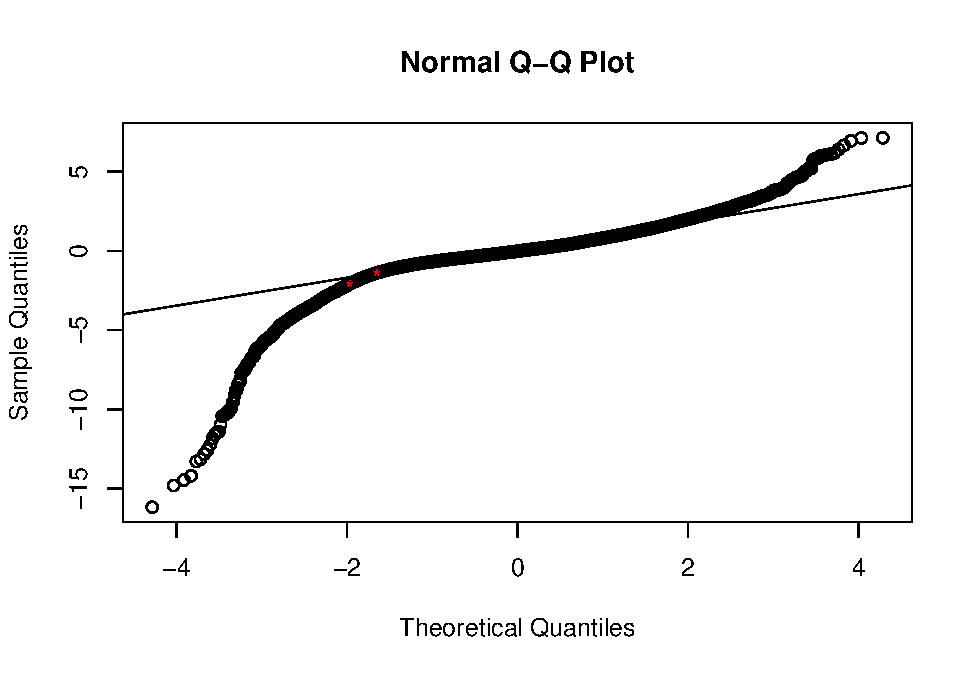
\includegraphics{13-MultipleLinearRegression_files/figure-latex/unnamed-chunk-9-1.pdf}

\hypertarget{addressing-non-constant-variance-using-wls}{%
\section{Addressing non-constant variance using WLS}\label{addressing-non-constant-variance-using-wls}}

Our increasing variance in residuals as a function of predicted price seems to have to do with carat. We can perform a weighted least squares estimation by weighting the observations by carat. The idea is that prices of diamonds with larger carat size have more variance, so we should downweight these observations compared to observations of smaller carat diamonds.\\
In R we can do this by using the lm() function with the wt option equal to 1/carat.
Using weights does not ``correct'' the non-constant variance; rather, we are incorporating the non-constant variance into the model.

\begin{Shaded}
\begin{Highlighting}[]
\NormalTok{get.weights }\OtherTok{\textless{}{-}} \FunctionTok{lm}\NormalTok{(full.lm.sqrt}\SpecialCharTok{$}\NormalTok{residuals}\SpecialCharTok{\^{}}\DecValTok{2} \SpecialCharTok{\textasciitilde{}}\NormalTok{ full.lm.sqrt}\SpecialCharTok{$}\NormalTok{fitted.values)}


\NormalTok{wls }\OtherTok{\textless{}{-}} \FunctionTok{lm}\NormalTok{(}\FunctionTok{sqrt}\NormalTok{(price)}\SpecialCharTok{\textasciitilde{}}\NormalTok{carat}\SpecialCharTok{+}\NormalTok{cut.num}\SpecialCharTok{+}\NormalTok{color.num}\SpecialCharTok{+}\NormalTok{clarity.num }\SpecialCharTok{+}\NormalTok{ carat}\SpecialCharTok{*}\NormalTok{clarity.num }\SpecialCharTok{+}\NormalTok{ carat}\SpecialCharTok{*}\NormalTok{color.num }\SpecialCharTok{+}\NormalTok{carat}\SpecialCharTok{*}\NormalTok{cut.num, }\AttributeTok{weights  =} \DecValTok{1}\SpecialCharTok{/}\NormalTok{diamonds}\SpecialCharTok{$}\NormalTok{carat, }\AttributeTok{data =}\NormalTok{ diamonds)}
\FunctionTok{summary}\NormalTok{(wls)}
\end{Highlighting}
\end{Shaded}

\begin{verbatim}
## 
## Call:
## lm(formula = sqrt(price) ~ carat + cut.num + color.num + clarity.num + 
##     carat * clarity.num + carat * color.num + carat * cut.num, 
##     data = diamonds, weights = 1/diamonds$carat)
## 
## Weighted Residuals:
##     Min      1Q  Median      3Q     Max 
## -45.644  -2.700  -0.031   2.874  42.921 
## 
## Coefficients:
##                   Estimate Std. Error  t value Pr(>|t|)    
## (Intercept)        3.82491    0.13972   27.376  < 2e-16 ***
## carat             54.59492    0.19776  276.068  < 2e-16 ***
## cut.num           -0.08956    0.02699   -3.318 0.000907 ***
## color.num          0.15453    0.01704    9.067  < 2e-16 ***
## clarity.num       -0.32964    0.01717  -19.199  < 2e-16 ***
## carat:clarity.num  5.21950    0.02755  189.471  < 2e-16 ***
## carat:color.num   -3.11506    0.02404 -129.588  < 2e-16 ***
## carat:cut.num      1.23565    0.03821   32.339  < 2e-16 ***
## ---
## Signif. codes:  0 '***' 0.001 '**' 0.01 '*' 0.05 '.' 0.1 ' ' 1
## 
## Residual standard error: 4.583 on 53932 degrees of freedom
## Multiple R-squared:  0.9764, Adjusted R-squared:  0.9764 
## F-statistic: 3.192e+05 on 7 and 53932 DF,  p-value: < 2.2e-16
\end{verbatim}

\begin{Shaded}
\begin{Highlighting}[]
\FunctionTok{AIC}\NormalTok{(wls)}
\end{Highlighting}
\end{Shaded}

\begin{verbatim}
## [1] 296006.8
\end{verbatim}

\begin{Shaded}
\begin{Highlighting}[]
\FunctionTok{BIC}\NormalTok{(wls)}
\end{Highlighting}
\end{Shaded}

\begin{verbatim}
## [1] 296086.8
\end{verbatim}

\begin{Shaded}
\begin{Highlighting}[]
\FunctionTok{qqnorm}\NormalTok{(wls}\SpecialCharTok{$}\NormalTok{residuals)}
\FunctionTok{qqline}\NormalTok{(wls}\SpecialCharTok{$}\NormalTok{residuals)}
\end{Highlighting}
\end{Shaded}

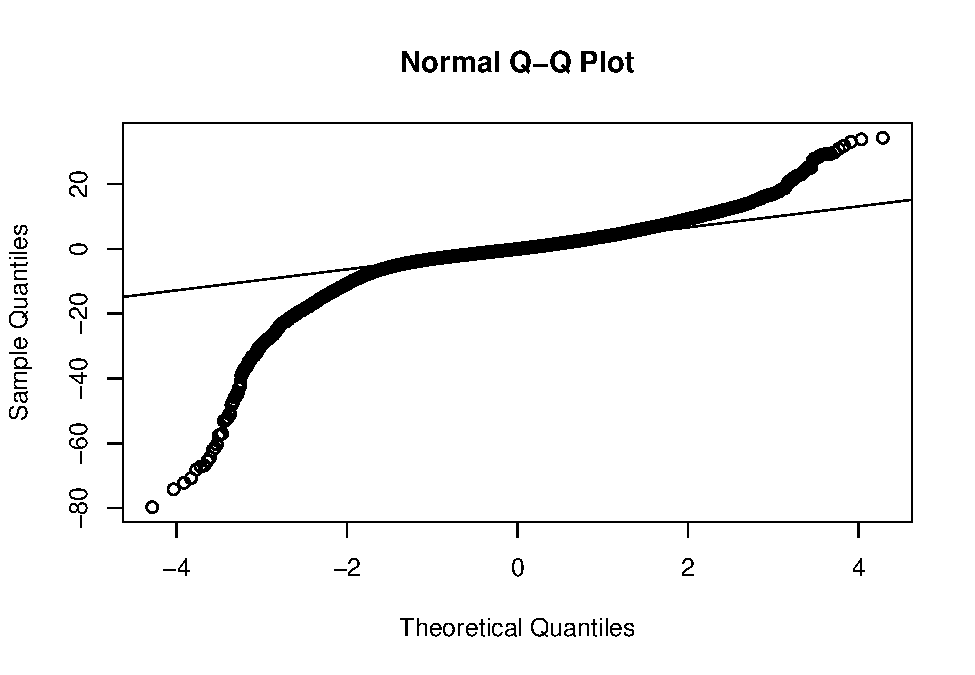
\includegraphics{13-MultipleLinearRegression_files/figure-latex/unnamed-chunk-10-1.pdf}

\begin{Shaded}
\begin{Highlighting}[]
\FunctionTok{plot}\NormalTok{(wls}\SpecialCharTok{$}\NormalTok{fitted.values,wls}\SpecialCharTok{$}\NormalTok{residuals) }
\end{Highlighting}
\end{Shaded}

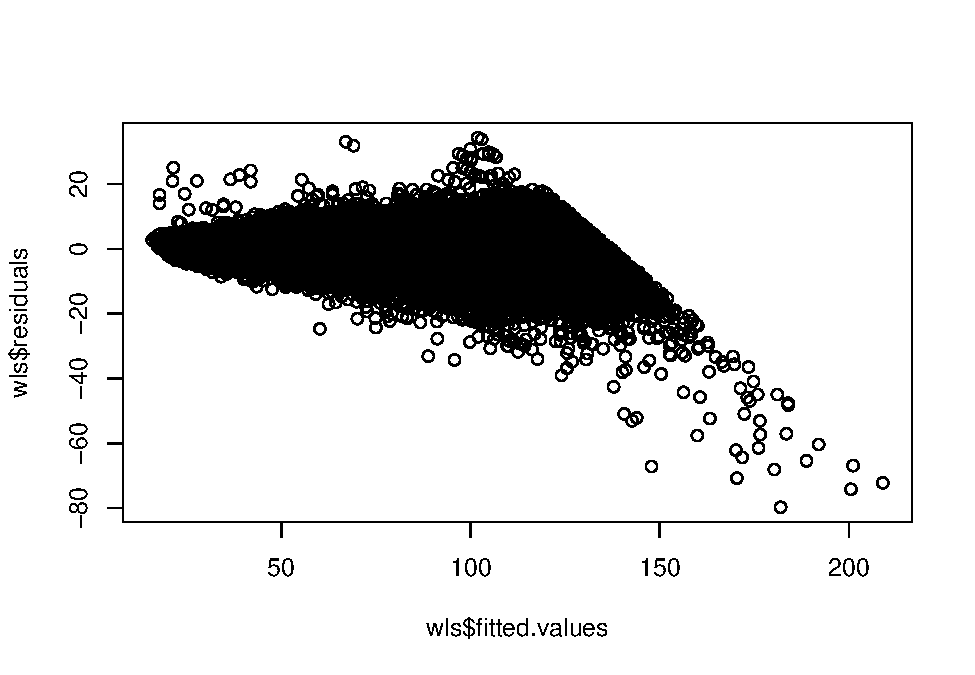
\includegraphics{13-MultipleLinearRegression_files/figure-latex/unnamed-chunk-10-2.pdf}

\begin{Shaded}
\begin{Highlighting}[]
\FunctionTok{plot}\NormalTok{(diamonds}\SpecialCharTok{$}\NormalTok{carat,wls}\SpecialCharTok{$}\NormalTok{residuals) }
\end{Highlighting}
\end{Shaded}

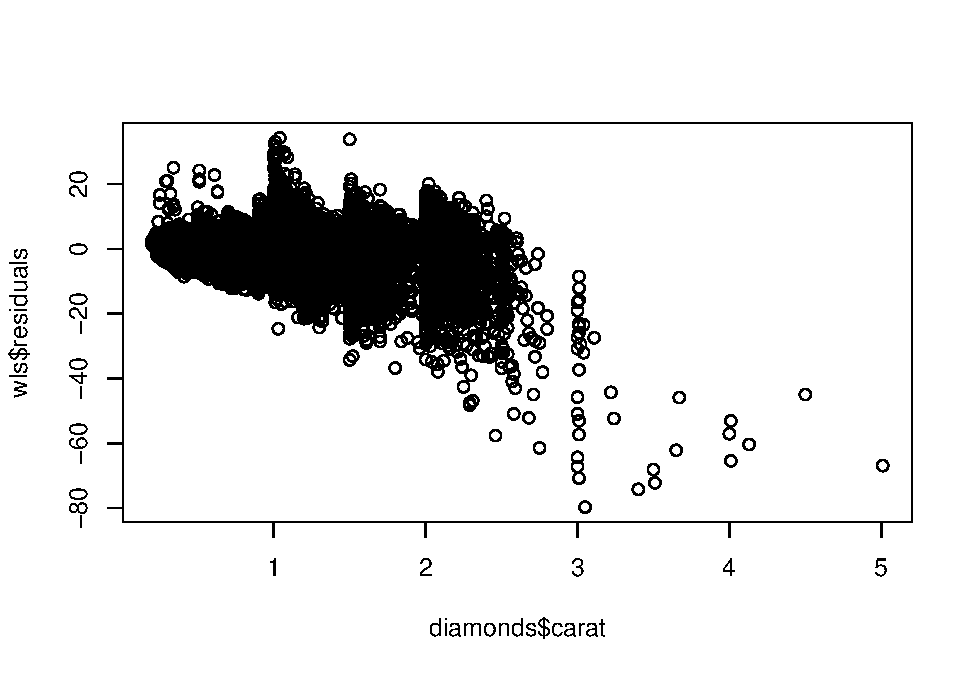
\includegraphics{13-MultipleLinearRegression_files/figure-latex/unnamed-chunk-10-3.pdf}

\hypertarget{inferences-using-wls}{%
\section{Inferences using WLS}\label{inferences-using-wls}}

Let's compare confidence/prediction intervals using the WLS and OLS models. The WLS inferences are more ``honest'' than the OLS inferences because the OLS model's assumption of constant variance is clearly violated. But, let's see what practical difference it makes.
1. 95\% CI for the carat beta
2. 95\% CI for mean price for carat = 1.5, cut = 3, clarity = 5, color = 2. This is a fairly large diamond of good quality.
3. 95\% Prediction interval for the same.

\begin{Shaded}
\begin{Highlighting}[]
\NormalTok{X }\OtherTok{\textless{}{-}} \FunctionTok{model.matrix}\NormalTok{(}\FunctionTok{sqrt}\NormalTok{(price)}\SpecialCharTok{\textasciitilde{}}\NormalTok{carat}\SpecialCharTok{+}\NormalTok{cut.num}\SpecialCharTok{+}\NormalTok{color.num}\SpecialCharTok{+}\NormalTok{clarity.num }\SpecialCharTok{+}\NormalTok{ carat}\SpecialCharTok{*}\NormalTok{clarity.num }\SpecialCharTok{+}\NormalTok{ carat}\SpecialCharTok{*}\NormalTok{color.num }\SpecialCharTok{+}\NormalTok{carat}\SpecialCharTok{*}\NormalTok{cut.num, }\AttributeTok{data=}\NormalTok{ diamonds)}
\NormalTok{Y }\OtherTok{\textless{}{-}} \FunctionTok{sqrt}\NormalTok{(diamonds}\SpecialCharTok{$}\NormalTok{price)}
\NormalTok{n }\OtherTok{\textless{}{-}} \FunctionTok{nrow}\NormalTok{(X)}
\NormalTok{p }\OtherTok{\textless{}{-}} \FunctionTok{ncol}\NormalTok{(X)}
\NormalTok{W }\OtherTok{\textless{}{-}}\NormalTok{ (}\DecValTok{1}\SpecialCharTok{/}\NormalTok{diamonds}\SpecialCharTok{$}\NormalTok{carat)}

\DocumentationTok{\#\#\# OLS inferences}
\NormalTok{XX.inv }\OtherTok{\textless{}{-}} \FunctionTok{solve}\NormalTok{(}\FunctionTok{t}\NormalTok{(X)}\SpecialCharTok{\%*\%}\NormalTok{X)}
\NormalTok{beta.hat.ols }\OtherTok{\textless{}{-}}\NormalTok{ XX.inv}\SpecialCharTok{\%*\%}\FunctionTok{t}\NormalTok{(X)}\SpecialCharTok{\%*\%}\NormalTok{Y}
\NormalTok{beta.hat.ols}
\end{Highlighting}
\end{Shaded}

\begin{verbatim}
##                         [,1]
## (Intercept)        5.3557161
## carat             52.8494746
## cut.num           -0.2356664
## color.num          0.4515624
## clarity.num       -0.6998048
## carat:clarity.num  5.6363319
## carat:color.num   -3.3927023
## carat:cut.num      1.3977070
\end{verbatim}

\begin{Shaded}
\begin{Highlighting}[]
\NormalTok{MSE.ols }\OtherTok{\textless{}{-}}\NormalTok{ (}\DecValTok{1}\SpecialCharTok{/}\NormalTok{(n}\SpecialCharTok{{-}}\NormalTok{p))}\SpecialCharTok{*}\FunctionTok{sum}\NormalTok{((Y }\SpecialCharTok{{-}}\NormalTok{ X}\SpecialCharTok{\%*\%}\NormalTok{beta.hat.ols)}\SpecialCharTok{\^{}}\DecValTok{2}\NormalTok{)}
\NormalTok{MSE.ols}
\end{Highlighting}
\end{Shaded}

\begin{verbatim}
## [1] 22.76062
\end{verbatim}

\begin{Shaded}
\begin{Highlighting}[]
\CommentTok{\# CI for carat beta}
\FunctionTok{c}\NormalTok{(beta.hat.ols[}\DecValTok{2}\NormalTok{] }\SpecialCharTok{{-}} \FunctionTok{qt}\NormalTok{(}\FloatTok{0.975}\NormalTok{, n}\SpecialCharTok{{-}}\NormalTok{p)}\SpecialCharTok{*}\FunctionTok{sqrt}\NormalTok{(MSE.ols}\SpecialCharTok{*}\NormalTok{XX.inv[}\DecValTok{2}\NormalTok{,}\DecValTok{2}\NormalTok{]), beta.hat.ols[}\DecValTok{2}\NormalTok{] }\SpecialCharTok{+} \FunctionTok{qt}\NormalTok{(}\FloatTok{0.975}\NormalTok{, n}\SpecialCharTok{{-}}\NormalTok{p)}\SpecialCharTok{*}\FunctionTok{sqrt}\NormalTok{(MSE.ols}\SpecialCharTok{*}\NormalTok{XX.inv[}\DecValTok{2}\NormalTok{,}\DecValTok{2}\NormalTok{]))}
\end{Highlighting}
\end{Shaded}

\begin{verbatim}
## [1] 52.44495 53.25400
\end{verbatim}

\begin{Shaded}
\begin{Highlighting}[]
\CommentTok{\# CI for mean price of that diamond}
\NormalTok{x }\OtherTok{\textless{}{-}} \FunctionTok{matrix}\NormalTok{(}\FunctionTok{c}\NormalTok{(}\DecValTok{1}\NormalTok{, }\FloatTok{1.5}\NormalTok{, }\DecValTok{3}\NormalTok{,}\DecValTok{2}\NormalTok{,}\DecValTok{5}\NormalTok{,}\FloatTok{1.5}\SpecialCharTok{*}\DecValTok{5}\NormalTok{, }\FloatTok{1.5}\SpecialCharTok{*}\DecValTok{2}\NormalTok{, }\FloatTok{1.5}\SpecialCharTok{*}\DecValTok{3}\NormalTok{), }\DecValTok{8}\NormalTok{,}\DecValTok{1}\NormalTok{)}
\FunctionTok{c}\NormalTok{(}\FunctionTok{t}\NormalTok{(x)}\SpecialCharTok{\%*\%}\NormalTok{beta.hat.ols }\SpecialCharTok{{-}} \FunctionTok{qt}\NormalTok{(}\FloatTok{0.975}\NormalTok{, n}\SpecialCharTok{{-}}\NormalTok{p)}\SpecialCharTok{*}\FunctionTok{sqrt}\NormalTok{(MSE.ols}\SpecialCharTok{*}\FunctionTok{t}\NormalTok{(x)}\SpecialCharTok{\%*\%}\NormalTok{XX.inv}\SpecialCharTok{\%*\%}\NormalTok{x), }\FunctionTok{t}\NormalTok{(x)}\SpecialCharTok{\%*\%}\NormalTok{beta.hat.ols }\SpecialCharTok{+} \FunctionTok{qt}\NormalTok{(}\FloatTok{0.975}\NormalTok{, n}\SpecialCharTok{{-}}\NormalTok{p)}\SpecialCharTok{*}\FunctionTok{sqrt}\NormalTok{(MSE.ols}\SpecialCharTok{*}\FunctionTok{t}\NormalTok{(x)}\SpecialCharTok{\%*\%}\NormalTok{XX.inv}\SpecialCharTok{\%*\%}\NormalTok{x))}
\end{Highlighting}
\end{Shaded}

\begin{verbatim}
## [1] 119.5424 119.8798
\end{verbatim}

\begin{Shaded}
\begin{Highlighting}[]
\CommentTok{\# PI}
\FunctionTok{c}\NormalTok{(}\FunctionTok{t}\NormalTok{(x)}\SpecialCharTok{\%*\%}\NormalTok{beta.hat.ols }\SpecialCharTok{{-}} \FunctionTok{qt}\NormalTok{(}\FloatTok{0.975}\NormalTok{, n}\SpecialCharTok{{-}}\NormalTok{p)}\SpecialCharTok{*}\FunctionTok{sqrt}\NormalTok{(MSE.ols}\SpecialCharTok{*}\NormalTok{(}\DecValTok{1}\SpecialCharTok{+}\FunctionTok{t}\NormalTok{(x)}\SpecialCharTok{\%*\%}\NormalTok{XX.inv}\SpecialCharTok{\%*\%}\NormalTok{x)), }\FunctionTok{t}\NormalTok{(x)}\SpecialCharTok{\%*\%}\NormalTok{beta.hat.ols }\SpecialCharTok{+} \FunctionTok{qt}\NormalTok{(}\FloatTok{0.975}\NormalTok{, n}\SpecialCharTok{{-}}\NormalTok{p)}\SpecialCharTok{*}\FunctionTok{sqrt}\NormalTok{(MSE.ols}\SpecialCharTok{*}\NormalTok{(}\DecValTok{1}\SpecialCharTok{+}\FunctionTok{t}\NormalTok{(x)}\SpecialCharTok{\%*\%}\NormalTok{XX.inv}\SpecialCharTok{\%*\%}\NormalTok{x)))}
\end{Highlighting}
\end{Shaded}

\begin{verbatim}
## [1] 110.3587 129.0634
\end{verbatim}

\begin{Shaded}
\begin{Highlighting}[]
\DocumentationTok{\#\#\# WLS inferences}
\NormalTok{XW }\OtherTok{\textless{}{-}} \FunctionTok{matrix}\NormalTok{(}\DecValTok{0}\NormalTok{,p,n)}
\NormalTok{tX }\OtherTok{\textless{}{-}} \FunctionTok{t}\NormalTok{(X)}
\ControlFlowTok{for}\NormalTok{(j }\ControlFlowTok{in} \DecValTok{1}\SpecialCharTok{:}\NormalTok{n)\{}
\NormalTok{  Wj }\OtherTok{\textless{}{-}} \FunctionTok{matrix}\NormalTok{(}\DecValTok{0}\NormalTok{,n,}\DecValTok{1}\NormalTok{)}
\NormalTok{  Wj[j] }\OtherTok{\textless{}{-}}\NormalTok{ W[j]}
\ControlFlowTok{for}\NormalTok{(i }\ControlFlowTok{in} \DecValTok{1}\SpecialCharTok{:}\NormalTok{p)\{}
\NormalTok{  XW[i,j] }\OtherTok{\textless{}{-}}\NormalTok{ tX[i,]}\SpecialCharTok{\%*\%}\NormalTok{Wj}
\NormalTok{\}}
\NormalTok{\}  }

\NormalTok{XWX.inv }\OtherTok{\textless{}{-}} \FunctionTok{solve}\NormalTok{(XW}\SpecialCharTok{\%*\%}\NormalTok{X)}



\NormalTok{beta.hat.wls }\OtherTok{\textless{}{-}}\NormalTok{ XWX.inv}\SpecialCharTok{\%*\%}\NormalTok{XW}\SpecialCharTok{\%*\%}\NormalTok{Y}
\NormalTok{beta.hat.wls}
\end{Highlighting}
\end{Shaded}

\begin{verbatim}
##                          [,1]
## (Intercept)        3.82491459
## carat             54.59491779
## cut.num           -0.08955524
## color.num          0.15452811
## clarity.num       -0.32964027
## carat:clarity.num  5.21950075
## carat:color.num   -3.11506184
## carat:cut.num      1.23564947
\end{verbatim}

\begin{Shaded}
\begin{Highlighting}[]
\NormalTok{MSE.wls }\OtherTok{\textless{}{-}}\NormalTok{ (}\DecValTok{1}\SpecialCharTok{/}\NormalTok{(n}\SpecialCharTok{{-}}\NormalTok{p))}\SpecialCharTok{*}\FunctionTok{sum}\NormalTok{(W}\SpecialCharTok{*}\NormalTok{(Y }\SpecialCharTok{{-}}\NormalTok{ X}\SpecialCharTok{\%*\%}\NormalTok{beta.hat.wls)}\SpecialCharTok{\^{}}\DecValTok{2}\NormalTok{)}
\NormalTok{MSE.wls}
\end{Highlighting}
\end{Shaded}

\begin{verbatim}
## [1] 21.00181
\end{verbatim}

\begin{Shaded}
\begin{Highlighting}[]
\FunctionTok{c}\NormalTok{(beta.hat.wls[}\DecValTok{2}\NormalTok{] }\SpecialCharTok{{-}} \FunctionTok{qt}\NormalTok{(}\FloatTok{0.975}\NormalTok{, n}\SpecialCharTok{{-}}\NormalTok{p)}\SpecialCharTok{*}\FunctionTok{sqrt}\NormalTok{(MSE.wls}\SpecialCharTok{*}\NormalTok{XWX.inv[}\DecValTok{2}\NormalTok{,}\DecValTok{2}\NormalTok{]), beta.hat.wls[}\DecValTok{2}\NormalTok{] }\SpecialCharTok{+} \FunctionTok{qt}\NormalTok{(}\FloatTok{0.975}\NormalTok{, n}\SpecialCharTok{{-}}\NormalTok{p)}\SpecialCharTok{*}\FunctionTok{sqrt}\NormalTok{(MSE.wls}\SpecialCharTok{*}\NormalTok{XWX.inv[}\DecValTok{2}\NormalTok{,}\DecValTok{2}\NormalTok{]))}
\end{Highlighting}
\end{Shaded}

\begin{verbatim}
##    carat    carat 
## 54.20731 54.98253
\end{verbatim}

\begin{Shaded}
\begin{Highlighting}[]
\FunctionTok{c}\NormalTok{(}\FunctionTok{t}\NormalTok{(x)}\SpecialCharTok{\%*\%}\NormalTok{beta.hat.wls }\SpecialCharTok{{-}} \FunctionTok{qt}\NormalTok{(}\FloatTok{0.975}\NormalTok{, n}\SpecialCharTok{{-}}\NormalTok{p)}\SpecialCharTok{*}\FunctionTok{sqrt}\NormalTok{(MSE.wls}\SpecialCharTok{*}\FunctionTok{t}\NormalTok{(x)}\SpecialCharTok{\%*\%}\NormalTok{XWX.inv}\SpecialCharTok{\%*\%}\NormalTok{x), }\FunctionTok{t}\NormalTok{(x)}\SpecialCharTok{\%*\%}\NormalTok{beta.hat.wls }\SpecialCharTok{+} \FunctionTok{qt}\NormalTok{(}\FloatTok{0.975}\NormalTok{, n}\SpecialCharTok{{-}}\NormalTok{p)}\SpecialCharTok{*}\FunctionTok{sqrt}\NormalTok{(MSE.wls}\SpecialCharTok{*}\FunctionTok{t}\NormalTok{(x)}\SpecialCharTok{\%*\%}\NormalTok{XWX.inv}\SpecialCharTok{\%*\%}\NormalTok{x))}
\end{Highlighting}
\end{Shaded}

\begin{verbatim}
## [1] 119.2983 119.6437
\end{verbatim}

\begin{Shaded}
\begin{Highlighting}[]
\FunctionTok{c}\NormalTok{(}\FunctionTok{t}\NormalTok{(x)}\SpecialCharTok{\%*\%}\NormalTok{beta.hat.wls }\SpecialCharTok{{-}} \FunctionTok{qt}\NormalTok{(}\FloatTok{0.975}\NormalTok{, n}\SpecialCharTok{{-}}\NormalTok{p)}\SpecialCharTok{*}\FunctionTok{sqrt}\NormalTok{(MSE.wls}\SpecialCharTok{*}\NormalTok{(}\DecValTok{1}\SpecialCharTok{+}\FunctionTok{t}\NormalTok{(x)}\SpecialCharTok{\%*\%}\NormalTok{XWX.inv}\SpecialCharTok{\%*\%}\NormalTok{x)), }\FunctionTok{t}\NormalTok{(x)}\SpecialCharTok{\%*\%}\NormalTok{beta.hat.wls }\SpecialCharTok{+} \FunctionTok{qt}\NormalTok{(}\FloatTok{0.975}\NormalTok{, n}\SpecialCharTok{{-}}\NormalTok{p)}\SpecialCharTok{*}\FunctionTok{sqrt}\NormalTok{(MSE.wls}\SpecialCharTok{*}\NormalTok{(}\DecValTok{1}\SpecialCharTok{+}\FunctionTok{t}\NormalTok{(x)}\SpecialCharTok{\%*\%}\NormalTok{XWX.inv}\SpecialCharTok{\%*\%}\NormalTok{x)))}
\end{Highlighting}
\end{Shaded}

\begin{verbatim}
## [1] 110.4870 128.4549
\end{verbatim}

\begin{Shaded}
\begin{Highlighting}[]
\FunctionTok{c}\NormalTok{(}\FunctionTok{t}\NormalTok{(x)}\SpecialCharTok{\%*\%}\NormalTok{beta.hat.wls }\SpecialCharTok{{-}} \FunctionTok{qt}\NormalTok{(}\FloatTok{0.975}\NormalTok{, n}\SpecialCharTok{{-}}\NormalTok{p)}\SpecialCharTok{*}\FunctionTok{sqrt}\NormalTok{(MSE.wls}\SpecialCharTok{*}\NormalTok{(}\FloatTok{1.5}\SpecialCharTok{+}\FunctionTok{t}\NormalTok{(x)}\SpecialCharTok{\%*\%}\NormalTok{XWX.inv}\SpecialCharTok{\%*\%}\NormalTok{x)), }\FunctionTok{t}\NormalTok{(x)}\SpecialCharTok{\%*\%}\NormalTok{beta.hat.wls }\SpecialCharTok{+} \FunctionTok{qt}\NormalTok{(}\FloatTok{0.975}\NormalTok{, n}\SpecialCharTok{{-}}\NormalTok{p)}\SpecialCharTok{*}\FunctionTok{sqrt}\NormalTok{(MSE.wls}\SpecialCharTok{*}\NormalTok{(}\FloatTok{1.5}\SpecialCharTok{+}\FunctionTok{t}\NormalTok{(x)}\SpecialCharTok{\%*\%}\NormalTok{XWX.inv}\SpecialCharTok{\%*\%}\NormalTok{x)))}
\end{Highlighting}
\end{Shaded}

\begin{verbatim}
## [1] 108.4686 130.4733
\end{verbatim}

\hypertarget{using-built-in-functions-in-r-for-inference}{%
\section{Using built-in functions in R for inference}\label{using-built-in-functions-in-r-for-inference}}

Make sure to use the weights option in predict.lm for predicting a new response based on the WLS regression model.

\begin{Shaded}
\begin{Highlighting}[]
\FunctionTok{confint}\NormalTok{(full.lm.sqrt)}
\end{Highlighting}
\end{Shaded}

\begin{verbatim}
##                        2.5 %     97.5 %
## (Intercept)        4.9753505  5.7360816
## carat             52.4449462 53.2540030
## cut.num           -0.3098125 -0.1615203
## color.num          0.4042664  0.4988584
## clarity.num       -0.7474246 -0.6521849
## carat:clarity.num  5.5803670  5.6922968
## carat:color.num   -3.4420565 -3.3433480
## carat:cut.num      1.3198461  1.4755679
\end{verbatim}

\begin{Shaded}
\begin{Highlighting}[]
\FunctionTok{confint}\NormalTok{(wls)}
\end{Highlighting}
\end{Shaded}

\begin{verbatim}
##                        2.5 %      97.5 %
## (Intercept)        3.5510712  4.09875801
## carat             54.2073087 54.98252686
## cut.num           -0.1424549 -0.03665554
## color.num          0.1211232  0.18793297
## clarity.num       -0.3632933 -0.29598725
## carat:clarity.num  5.1655068  5.27349466
## carat:color.num   -3.1621770 -3.06794668
## carat:cut.num      1.1607589  1.31054002
\end{verbatim}

\begin{Shaded}
\begin{Highlighting}[]
\NormalTok{new.carat }\OtherTok{=} \FloatTok{1.5}
\NormalTok{new.cut }\OtherTok{=} \DecValTok{3}
\NormalTok{new.clarity }\OtherTok{=} \DecValTok{5}
\NormalTok{new.color }\OtherTok{=} \DecValTok{2}
\NormalTok{new.data }\OtherTok{\textless{}{-}} \FunctionTok{data.frame}\NormalTok{(}\AttributeTok{carat =}\NormalTok{ new.carat, }\AttributeTok{cut.num =}\NormalTok{ new.cut, }\AttributeTok{color.num =}\NormalTok{ new.color, }\AttributeTok{clarity.num =}\NormalTok{ new.clarity)}
\FunctionTok{predict.lm}\NormalTok{(wls, }\AttributeTok{newdata =}\NormalTok{ new.data, }\AttributeTok{interval =} \StringTok{\textquotesingle{}confidence\textquotesingle{}}\NormalTok{)}
\end{Highlighting}
\end{Shaded}

\begin{verbatim}
##       fit      lwr      upr
## 1 119.471 119.2983 119.6437
\end{verbatim}

\begin{Shaded}
\begin{Highlighting}[]
\FunctionTok{predict.lm}\NormalTok{(wls, }\AttributeTok{newdata =}\NormalTok{ new.data, }\AttributeTok{interval =} \StringTok{\textquotesingle{}prediction\textquotesingle{}}\NormalTok{)}
\end{Highlighting}
\end{Shaded}

\begin{verbatim}
## Warning in predict.lm(wls, newdata = new.data, interval = "prediction"): Assuming constant prediction variance even though model fit is weighted
\end{verbatim}

\begin{verbatim}
##       fit     lwr      upr
## 1 119.471 110.487 128.4549
\end{verbatim}

\begin{Shaded}
\begin{Highlighting}[]
\FunctionTok{predict.lm}\NormalTok{(wls, }\AttributeTok{newdata =}\NormalTok{ new.data, }\AttributeTok{interval =} \StringTok{\textquotesingle{}prediction\textquotesingle{}}\NormalTok{, }\AttributeTok{weights =} \DecValTok{1}\SpecialCharTok{/}\FloatTok{1.5}\NormalTok{)}
\end{Highlighting}
\end{Shaded}

\begin{verbatim}
##       fit      lwr      upr
## 1 119.471 108.4686 130.4733
\end{verbatim}

\begin{Shaded}
\begin{Highlighting}[]
\FunctionTok{predict.lm}\NormalTok{(full.lm.sqrt, }\AttributeTok{newdata =}\NormalTok{ new.data, }\AttributeTok{interval =} \StringTok{\textquotesingle{}confidence\textquotesingle{}}\NormalTok{)}
\end{Highlighting}
\end{Shaded}

\begin{verbatim}
##        fit      lwr      upr
## 1 119.7111 119.5424 119.8798
\end{verbatim}

\begin{Shaded}
\begin{Highlighting}[]
\FunctionTok{predict.lm}\NormalTok{(full.lm.sqrt, }\AttributeTok{newdata =}\NormalTok{ new.data, }\AttributeTok{interval =} \StringTok{\textquotesingle{}prediction\textquotesingle{}}\NormalTok{)}
\end{Highlighting}
\end{Shaded}

\begin{verbatim}
##        fit      lwr      upr
## 1 119.7111 110.3587 129.0634
\end{verbatim}

\hypertarget{leverage-outliers-and-influence}{%
\section{Leverage, outliers, and influence}\label{leverage-outliers-and-influence}}

Outlier are observations with very large residuals---the model is not good at predicting the prices of these diamonds. Large residuals may happen by chance, because the model is missing important covariate information, or because one or more assumptions are violated. Often, we consider removing observations with large residuals based on the rationale that if the model is not good at predicting those responses then those observations should not be modeled---a rationale that is, at least partially, flawed. Outlier observations are only troublesome if they have an outsized effect on the fit of the model, which may be measured by comparing \(\hat\beta\) with and without the observation in question, or comparing \(\hat Y\) or the \(SSE\). Observations that strongly affect the fit of the model have high \emph{leverage}. Outliers with high leverage are \emph{influential} points. It is only these influential points we need to worry about in terms of whether or not to include them in the model at all. On the other hand, outliers that are not influential are only important when it comes to interpreting the fit of the model at that particular observation, and not for interpreting the model in general.

\hypertarget{illustrations}{%
\subsection{Illustrations}\label{illustrations}}

First, some ``cartoons'' or ``toy'' examples. The following plots illustrate outliers, leverage, and influence using a simple linear regression on contrived data. The first plot shows a fit without any outliers. The second shows a fit with a high leverage point, that is not an outlier. The third show a pair of fitterd lines with and without a non-influential outlier (one without leverage). And, the fourth shows a plot of a pair of fitted lines with and without an influential point.

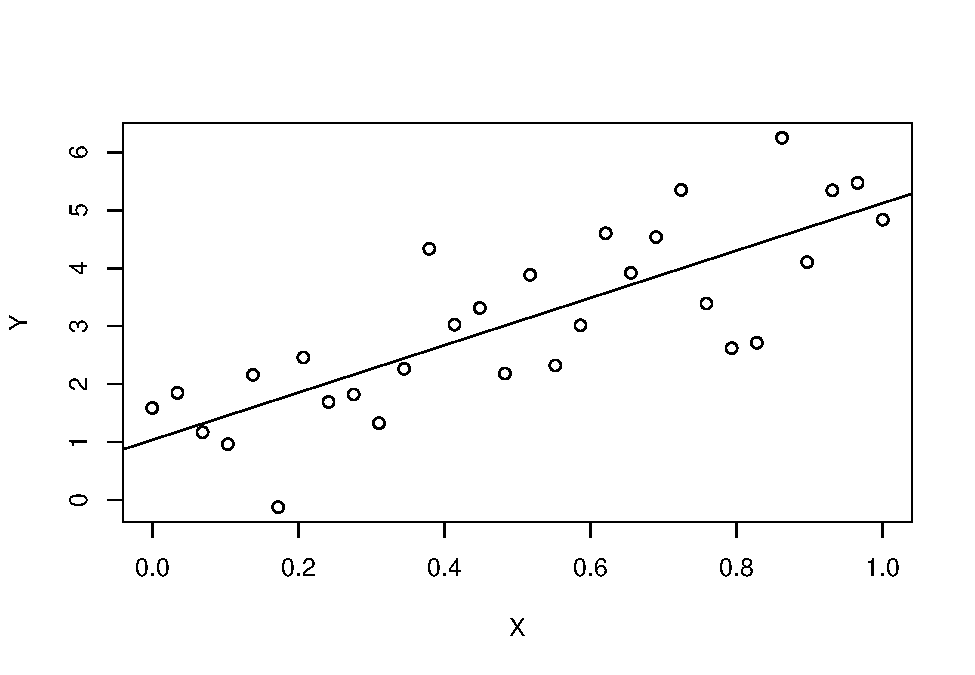
\includegraphics{13-MultipleLinearRegression_files/figure-latex/unnamed-chunk-13-1.pdf}

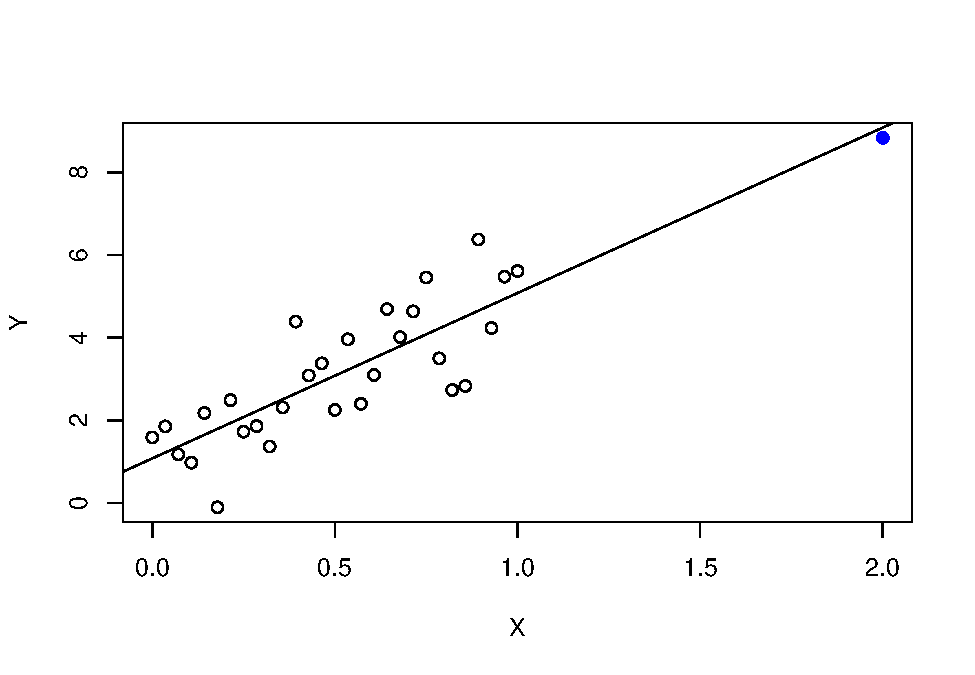
\includegraphics{13-MultipleLinearRegression_files/figure-latex/unnamed-chunk-14-1.pdf}

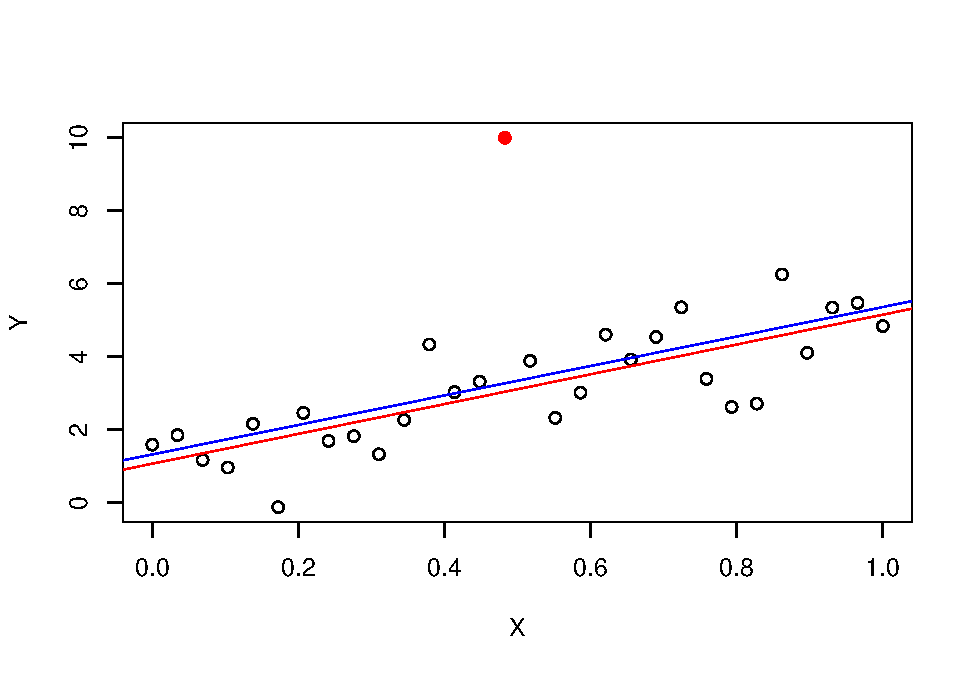
\includegraphics{13-MultipleLinearRegression_files/figure-latex/unnamed-chunk-15-1.pdf}

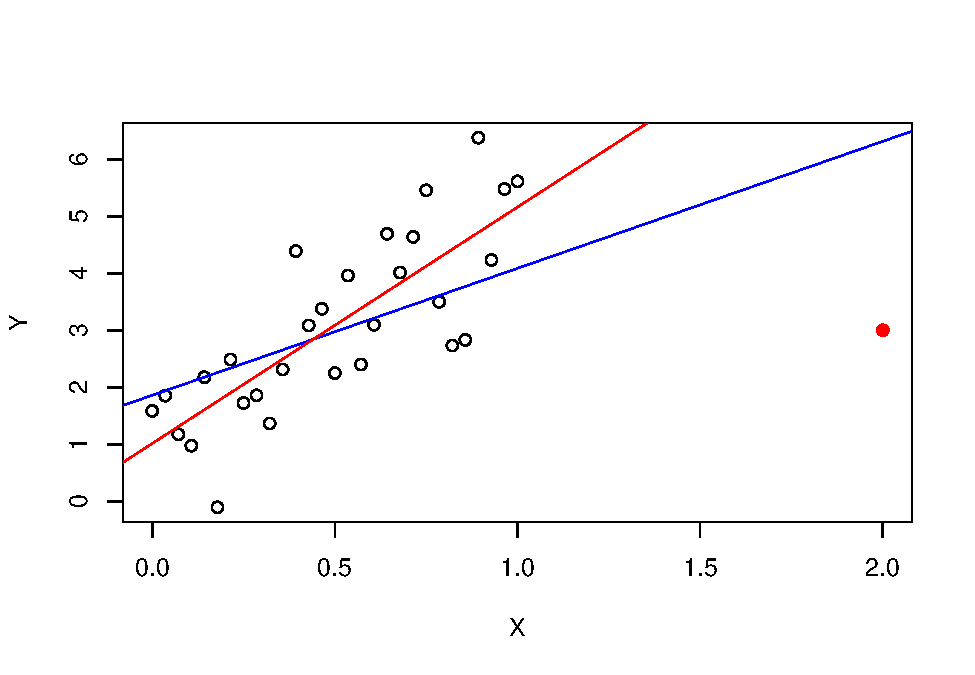
\includegraphics{13-MultipleLinearRegression_files/figure-latex/unnamed-chunk-16-1.pdf}

\hypertarget{numerical-summaries-of-outliers-leverage-and-influence}{%
\section{Numerical summaries of outliers, leverage, and influence}\label{numerical-summaries-of-outliers-leverage-and-influence}}

The ``hat'' matrix \(H = X(X^\top X)^{-1}X^\top\) determines high leverage points. To see this, note that the fitted responses are given by \(\hat Y = H Y\), which are linear combinations of all the responses. We can express \(\hat Y_i\)---the predicted price of the \(i^{th}\) diamond---as a linear combination of the price of the \(i^{th}\) diamond itself and the other \(n-1\) diamonds: \(\hat Y_i = h_{ii}Y_i + \sum_{i\ne j} h_{ij}Y_j\) where \(h_{ij}\) is the \(ij\) entry of \(H\). If we simply define leverage to be the degree to which an observed response determines its own prediction (or fitted value) then \(h_{ii}\)---the diagonal of \(H\)---defines leverage.

\begin{Shaded}
\begin{Highlighting}[]
\NormalTok{h.X }\OtherTok{\textless{}{-}} \FunctionTok{hat}\NormalTok{(X)}
\NormalTok{h.X}
\end{Highlighting}
\end{Shaded}

\begin{verbatim}
##  [1] 0.09682659 0.08884843 0.08140573 0.07449847 0.06812665 0.06229028
##  [7] 0.05698936 0.05222389 0.04799386 0.04429928 0.04114014 0.03851646
## [13] 0.03642821 0.03487542 0.03385807 0.03337617 0.03342971 0.03401870
## [19] 0.03514314 0.03680303 0.03899836 0.04172914 0.04499536 0.04879703
## [25] 0.05313415 0.05800671 0.06341472 0.06935818 0.07583708 0.47463768
\end{verbatim}

\begin{Shaded}
\begin{Highlighting}[]
\CommentTok{\# hat(model.matrix(Y\textasciitilde{}X))   \# same}
\FunctionTok{which}\NormalTok{(h.X }\SpecialCharTok{\textgreater{}}\NormalTok{ (}\DecValTok{3}\SpecialCharTok{*}\DecValTok{2} \SpecialCharTok{/} \DecValTok{30}\NormalTok{))   }\CommentTok{\# 3(k+1)/n}
\end{Highlighting}
\end{Shaded}

\begin{verbatim}
## [1] 30
\end{verbatim}

\begin{Shaded}
\begin{Highlighting}[]
\FunctionTok{which.max}\NormalTok{(h.X)}
\end{Highlighting}
\end{Shaded}

\begin{verbatim}
## [1] 30
\end{verbatim}

\begin{Shaded}
\begin{Highlighting}[]
\CommentTok{\# "by hand"}
\NormalTok{X.d }\OtherTok{\textless{}{-}} \FunctionTok{cbind}\NormalTok{(}\FunctionTok{rep}\NormalTok{(}\DecValTok{1}\NormalTok{,}\DecValTok{30}\NormalTok{),X)}
\NormalTok{hat.X }\OtherTok{\textless{}{-}}\NormalTok{ X.d}\SpecialCharTok{\%*\%}\FunctionTok{solve}\NormalTok{(}\FunctionTok{t}\NormalTok{(X.d)}\SpecialCharTok{\%*\%}\NormalTok{X.d)}\SpecialCharTok{\%*\%}\FunctionTok{t}\NormalTok{(X.d)  }\CommentTok{\# n by n matrix}
\FunctionTok{diag}\NormalTok{(hat.X)}
\end{Highlighting}
\end{Shaded}

\begin{verbatim}
##  [1] 0.09682659 0.08884843 0.08140573 0.07449847 0.06812665 0.06229028
##  [7] 0.05698936 0.05222389 0.04799386 0.04429928 0.04114014 0.03851646
## [13] 0.03642821 0.03487542 0.03385807 0.03337617 0.03342971 0.03401870
## [19] 0.03514314 0.03680303 0.03899836 0.04172914 0.04499536 0.04879703
## [25] 0.05313415 0.05800671 0.06341472 0.06935818 0.07583708 0.47463768
\end{verbatim}

Outliers are defined by large residuals. In multiple linear regression there is more than one way to define residuals and studentized residuals. ``Studentized'' refers to normalizing residuals by the estimated standard deviation. Internally studentized residuals include each observation in the calculation of the estimated standard deviation whereas externally studentized residuals ignore the corresponding observation when computing the estimated standard deviation for normalization.

\begin{Shaded}
\begin{Highlighting}[]
\FunctionTok{plot}\NormalTok{(X, my.lm}\SpecialCharTok{$}\NormalTok{residuals)}
\end{Highlighting}
\end{Shaded}

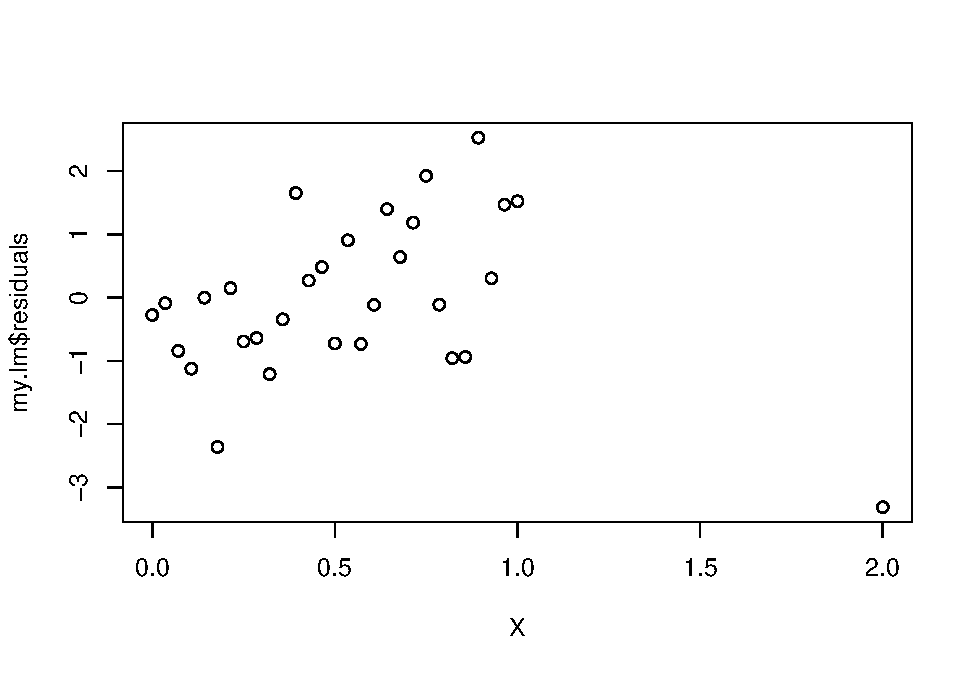
\includegraphics{13-MultipleLinearRegression_files/figure-latex/unnamed-chunk-18-1.pdf}

\begin{Shaded}
\begin{Highlighting}[]
\NormalTok{MSE }\OtherTok{\textless{}{-}} \FunctionTok{sum}\NormalTok{(my.lm}\SpecialCharTok{$}\NormalTok{residuals}\SpecialCharTok{\^{}}\DecValTok{2}\NormalTok{)}\SpecialCharTok{/}\NormalTok{(}\DecValTok{30{-}2}\NormalTok{)}
\NormalTok{int.stud.resids }\OtherTok{\textless{}{-}}\NormalTok{ my.lm}\SpecialCharTok{$}\NormalTok{residuals }\SpecialCharTok{/} \FunctionTok{sqrt}\NormalTok{(MSE }\SpecialCharTok{*}\NormalTok{ (}\DecValTok{1}\SpecialCharTok{{-}}\NormalTok{h.X))}
\FunctionTok{plot}\NormalTok{(X, int.stud.resids)}
\end{Highlighting}
\end{Shaded}

\includegraphics{13-MultipleLinearRegression_files/figure-latex/unnamed-chunk-18-2.pdf}

\begin{Shaded}
\begin{Highlighting}[]
\NormalTok{MSE.i }\OtherTok{\textless{}{-}} \FunctionTok{rep}\NormalTok{(}\ConstantTok{NA}\NormalTok{, }\DecValTok{30}\NormalTok{)}
\ControlFlowTok{for}\NormalTok{(i }\ControlFlowTok{in} \DecValTok{1}\SpecialCharTok{:}\DecValTok{30}\NormalTok{)\{}
\NormalTok{MSE.i[i] }\OtherTok{\textless{}{-}} \FunctionTok{sum}\NormalTok{(my.lm}\SpecialCharTok{$}\NormalTok{residuals[}\SpecialCharTok{{-}}\NormalTok{i]}\SpecialCharTok{\^{}}\DecValTok{2}\NormalTok{)}\SpecialCharTok{/}\NormalTok{(}\DecValTok{30{-}2{-}1}\NormalTok{)}
\NormalTok{\}}
\NormalTok{ext.stud.resids }\OtherTok{\textless{}{-}}\NormalTok{ my.lm}\SpecialCharTok{$}\NormalTok{residuals }\SpecialCharTok{/} \FunctionTok{sqrt}\NormalTok{(MSE.i }\SpecialCharTok{*}\NormalTok{ (}\DecValTok{1}\SpecialCharTok{{-}}\NormalTok{h.X))}
\FunctionTok{plot}\NormalTok{(X, ext.stud.resids)}
\end{Highlighting}
\end{Shaded}

\includegraphics{13-MultipleLinearRegression_files/figure-latex/unnamed-chunk-18-3.pdf}

An observation's \emph{influence} can be defined by the degree to which is affects the model through \(\hat\beta\) or \(\hat Y\). Cook's D and DfFits measure the fit of the model, which is related to residuals and fitted/predicted values, whereas DfBetas measures the change in the fitted coefficients with or without the given observation.

\begin{Shaded}
\begin{Highlighting}[]
\CommentTok{\# base r functions}
\NormalTok{cd }\OtherTok{\textless{}{-}} \FunctionTok{cooks.distance}\NormalTok{(my.lm)}
\FunctionTok{which}\NormalTok{(cd }\SpecialCharTok{\textgreater{}} \DecValTok{2}\SpecialCharTok{*}\FunctionTok{sqrt}\NormalTok{(}\DecValTok{2}\SpecialCharTok{/}\DecValTok{30}\NormalTok{))}
\end{Highlighting}
\end{Shaded}

\begin{verbatim}
## 30 
## 30
\end{verbatim}

\begin{Shaded}
\begin{Highlighting}[]
\NormalTok{dfb }\OtherTok{\textless{}{-}} \FunctionTok{dfbetas}\NormalTok{(my.lm)}
\FunctionTok{which}\NormalTok{(dfb }\SpecialCharTok{\textgreater{}} \DecValTok{2}\NormalTok{)}
\end{Highlighting}
\end{Shaded}

\begin{verbatim}
## [1] 30
\end{verbatim}

\begin{Shaded}
\begin{Highlighting}[]
\NormalTok{dff }\OtherTok{\textless{}{-}} \FunctionTok{dffits}\NormalTok{(my.lm)}
\FunctionTok{which}\NormalTok{(dff }\SpecialCharTok{\textgreater{}} \DecValTok{2}\SpecialCharTok{*}\FunctionTok{sqrt}\NormalTok{(}\DecValTok{2}\SpecialCharTok{/}\DecValTok{30}\NormalTok{))}
\end{Highlighting}
\end{Shaded}

\begin{verbatim}
## 26 
## 26
\end{verbatim}

\begin{Shaded}
\begin{Highlighting}[]
\FunctionTok{library}\NormalTok{(olsrr)}
\end{Highlighting}
\end{Shaded}

\begin{verbatim}
## Warning: package 'olsrr' was built under R version 4.2.2
\end{verbatim}

\begin{verbatim}
## 
## Attaching package: 'olsrr'
\end{verbatim}

\begin{verbatim}
## The following object is masked from 'package:datasets':
## 
##     rivers
\end{verbatim}

\begin{Shaded}
\begin{Highlighting}[]
\FunctionTok{ols\_plot\_cooksd\_bar}\NormalTok{(my.lm)  }\CommentTok{\# lol}
\end{Highlighting}
\end{Shaded}

\includegraphics{13-MultipleLinearRegression_files/figure-latex/unnamed-chunk-19-1.pdf}

\begin{Shaded}
\begin{Highlighting}[]
\FunctionTok{ols\_plot\_dfbetas}\NormalTok{(my.lm)}
\end{Highlighting}
\end{Shaded}

\includegraphics{13-MultipleLinearRegression_files/figure-latex/unnamed-chunk-19-2.pdf}

\begin{Shaded}
\begin{Highlighting}[]
\FunctionTok{ols\_plot\_dffits}\NormalTok{(my.lm)}
\end{Highlighting}
\end{Shaded}

\includegraphics{13-MultipleLinearRegression_files/figure-latex/unnamed-chunk-19-3.pdf}

\hypertarget{leverage-diamonds-model}{%
\section{Leverage, Diamonds model}\label{leverage-diamonds-model}}

\begin{Shaded}
\begin{Highlighting}[]
\NormalTok{wls }\OtherTok{\textless{}{-}} \FunctionTok{lm}\NormalTok{(}\FunctionTok{sqrt}\NormalTok{(price)}\SpecialCharTok{\textasciitilde{}}\NormalTok{carat}\SpecialCharTok{+}\NormalTok{cut.num}\SpecialCharTok{+}\NormalTok{color.num}\SpecialCharTok{+}\NormalTok{clarity.num }\SpecialCharTok{+}\NormalTok{ carat}\SpecialCharTok{*}\NormalTok{clarity.num }\SpecialCharTok{+}\NormalTok{ carat}\SpecialCharTok{*}\NormalTok{color.num }\SpecialCharTok{+}\NormalTok{carat}\SpecialCharTok{*}\NormalTok{cut.num, }\AttributeTok{weights  =} \DecValTok{1}\SpecialCharTok{/}\NormalTok{diamonds}\SpecialCharTok{$}\NormalTok{carat, }\AttributeTok{data =}\NormalTok{ diamonds)}

\NormalTok{MSE.wls }\OtherTok{\textless{}{-}} \FunctionTok{sum}\NormalTok{((wls}\SpecialCharTok{$}\NormalTok{residuals)}\SpecialCharTok{\^{}}\DecValTok{2}\NormalTok{)}\SpecialCharTok{/}\NormalTok{(}\FunctionTok{nrow}\NormalTok{(diamonds)}\SpecialCharTok{{-}}\DecValTok{8}\NormalTok{)}

\NormalTok{leverages.lm }\OtherTok{\textless{}{-}} \FunctionTok{lm.influence}\NormalTok{(wls)}\SpecialCharTok{$}\NormalTok{hat}

\CommentTok{\# k + 1  = 8 fitted regression coefficients}
\CommentTok{\# n = 53940}

\DecValTok{3} \SpecialCharTok{*} \DecValTok{8}\SpecialCharTok{/}\DecValTok{53940}
\end{Highlighting}
\end{Shaded}

\begin{verbatim}
## [1] 0.0004449388
\end{verbatim}

\begin{Shaded}
\begin{Highlighting}[]
\FunctionTok{sum}\NormalTok{(leverages.lm }\SpecialCharTok{\textgreater{}} \FloatTok{0.00045}\NormalTok{)}
\end{Highlighting}
\end{Shaded}

\begin{verbatim}
## [1] 1248
\end{verbatim}

\begin{Shaded}
\begin{Highlighting}[]
\FunctionTok{sum}\NormalTok{(leverages.lm }\SpecialCharTok{\textgreater{}} \FloatTok{0.00045}\NormalTok{) }\SpecialCharTok{/} \DecValTok{53940}
\end{Highlighting}
\end{Shaded}

\begin{verbatim}
## [1] 0.02313682
\end{verbatim}

\begin{Shaded}
\begin{Highlighting}[]
\FunctionTok{plot}\NormalTok{(wls}\SpecialCharTok{$}\NormalTok{fitted.values[leverages.lm }\SpecialCharTok{\textless{}} \FloatTok{0.00045}\NormalTok{], wls}\SpecialCharTok{$}\NormalTok{residuals[leverages.lm }\SpecialCharTok{\textless{}} \FloatTok{0.00045}\NormalTok{])}
\FunctionTok{points}\NormalTok{(wls}\SpecialCharTok{$}\NormalTok{fitted.values[leverages.lm }\SpecialCharTok{\textgreater{}} \FloatTok{0.00045}\NormalTok{], wls}\SpecialCharTok{$}\NormalTok{residuals[leverages.lm }\SpecialCharTok{\textgreater{}} \FloatTok{0.00045}\NormalTok{], }\AttributeTok{col =} \StringTok{\textquotesingle{}blue\textquotesingle{}}\NormalTok{)}
\end{Highlighting}
\end{Shaded}

\includegraphics{13-MultipleLinearRegression_files/figure-latex/unnamed-chunk-20-1.pdf}

\hypertarget{outliers-diamonds-model}{%
\subsection{Outliers, diamonds model}\label{outliers-diamonds-model}}

\begin{Shaded}
\begin{Highlighting}[]
\NormalTok{int.stud.resids }\OtherTok{\textless{}{-}}\NormalTok{ wls}\SpecialCharTok{$}\NormalTok{residuals }\SpecialCharTok{/} \FunctionTok{sqrt}\NormalTok{(MSE.wls }\SpecialCharTok{*}\NormalTok{ (}\DecValTok{1}\SpecialCharTok{{-}}\NormalTok{leverages.lm))}
\FunctionTok{plot}\NormalTok{(wls}\SpecialCharTok{$}\NormalTok{fitted.values, int.stud.resids)}
\FunctionTok{points}\NormalTok{(wls}\SpecialCharTok{$}\NormalTok{fitted.values[}\FunctionTok{abs}\NormalTok{(int.stud.resids)}\SpecialCharTok{\textgreater{}}\DecValTok{3}\NormalTok{], int.stud.resids[}\FunctionTok{abs}\NormalTok{(int.stud.resids)}\SpecialCharTok{\textgreater{}}\DecValTok{3}\NormalTok{], }\AttributeTok{col =} \StringTok{\textquotesingle{}blue\textquotesingle{}}\NormalTok{)}
\end{Highlighting}
\end{Shaded}

\includegraphics{13-MultipleLinearRegression_files/figure-latex/unnamed-chunk-21-1.pdf}

\begin{Shaded}
\begin{Highlighting}[]
\NormalTok{MSE.i }\OtherTok{\textless{}{-}} \FunctionTok{rep}\NormalTok{(}\ConstantTok{NA}\NormalTok{, }\DecValTok{53940}\NormalTok{)}
\ControlFlowTok{for}\NormalTok{(i }\ControlFlowTok{in} \DecValTok{1}\SpecialCharTok{:}\DecValTok{53940}\NormalTok{)\{}
\NormalTok{MSE.i[i] }\OtherTok{\textless{}{-}} \FunctionTok{sum}\NormalTok{(wls}\SpecialCharTok{$}\NormalTok{residuals[}\SpecialCharTok{{-}}\NormalTok{i]}\SpecialCharTok{\^{}}\DecValTok{2}\NormalTok{)}\SpecialCharTok{/}\NormalTok{(}\DecValTok{53940{-}8{-}1}\NormalTok{)}
\NormalTok{\}}
\NormalTok{ext.stud.resids }\OtherTok{\textless{}{-}}\NormalTok{ wls}\SpecialCharTok{$}\NormalTok{residuals }\SpecialCharTok{/} \FunctionTok{sqrt}\NormalTok{(MSE.i }\SpecialCharTok{*}\NormalTok{ (}\DecValTok{1}\SpecialCharTok{{-}}\NormalTok{leverages.lm))}
\FunctionTok{plot}\NormalTok{(wls}\SpecialCharTok{$}\NormalTok{fitted.values, ext.stud.resids)}
\FunctionTok{points}\NormalTok{(wls}\SpecialCharTok{$}\NormalTok{fitted.values[}\FunctionTok{abs}\NormalTok{(ext.stud.resids)}\SpecialCharTok{\textgreater{}}\DecValTok{3}\NormalTok{], ext.stud.resids[}\FunctionTok{abs}\NormalTok{(ext.stud.resids)}\SpecialCharTok{\textgreater{}}\DecValTok{3}\NormalTok{], }\AttributeTok{col =} \StringTok{\textquotesingle{}blue\textquotesingle{}}\NormalTok{)}
\end{Highlighting}
\end{Shaded}

\includegraphics{13-MultipleLinearRegression_files/figure-latex/unnamed-chunk-21-2.pdf}

\hypertarget{plotting-outliers-with-leverage}{%
\subsection{plotting outliers with leverage}\label{plotting-outliers-with-leverage}}

\begin{Shaded}
\begin{Highlighting}[]
\FunctionTok{plot}\NormalTok{(wls}\SpecialCharTok{$}\NormalTok{fitted.values, ext.stud.resids)}
\FunctionTok{points}\NormalTok{(wls}\SpecialCharTok{$}\NormalTok{fitted.values[}\FunctionTok{abs}\NormalTok{(ext.stud.resids)}\SpecialCharTok{\textgreater{}}\DecValTok{3} \SpecialCharTok{\&}\NormalTok{ leverages.lm }\SpecialCharTok{\textgreater{}} \FloatTok{0.00045}\NormalTok{], ext.stud.resids[}\FunctionTok{abs}\NormalTok{(ext.stud.resids)}\SpecialCharTok{\textgreater{}}\DecValTok{3} \SpecialCharTok{\&}\NormalTok{ leverages.lm }\SpecialCharTok{\textgreater{}} \FloatTok{0.00045}\NormalTok{], }\AttributeTok{col =} \StringTok{\textquotesingle{}red\textquotesingle{}}\NormalTok{)}
\end{Highlighting}
\end{Shaded}

\includegraphics{13-MultipleLinearRegression_files/figure-latex/unnamed-chunk-22-1.pdf}

\begin{Shaded}
\begin{Highlighting}[]
\FunctionTok{length}\NormalTok{(wls}\SpecialCharTok{$}\NormalTok{fitted.values[}\FunctionTok{abs}\NormalTok{(ext.stud.resids)}\SpecialCharTok{\textgreater{}}\DecValTok{3} \SpecialCharTok{\&}\NormalTok{ leverages.lm }\SpecialCharTok{\textgreater{}} \FloatTok{0.00045}\NormalTok{])}
\end{Highlighting}
\end{Shaded}

\begin{verbatim}
## [1] 308
\end{verbatim}

\begin{Shaded}
\begin{Highlighting}[]
\FunctionTok{length}\NormalTok{(wls}\SpecialCharTok{$}\NormalTok{fitted.values[}\FunctionTok{abs}\NormalTok{(ext.stud.resids)}\SpecialCharTok{\textgreater{}}\DecValTok{3} \SpecialCharTok{\&}\NormalTok{ leverages.lm }\SpecialCharTok{\textgreater{}} \FloatTok{0.00045}\NormalTok{])}\SpecialCharTok{/}\DecValTok{53940}
\end{Highlighting}
\end{Shaded}

\begin{verbatim}
## [1] 0.005710048
\end{verbatim}

\hypertarget{cooks-distance-df-betas-df-fits}{%
\subsection{Cook's distance, DF betas, DF fits}\label{cooks-distance-df-betas-df-fits}}

\begin{Shaded}
\begin{Highlighting}[]
\CommentTok{\# base r functions}
\NormalTok{cd }\OtherTok{\textless{}{-}} \FunctionTok{cooks.distance}\NormalTok{(wls, }\AttributeTok{weights  =} \DecValTok{1}\SpecialCharTok{/}\NormalTok{diamonds}\SpecialCharTok{$}\NormalTok{carat)}
\FunctionTok{sum}\NormalTok{(cd }\SpecialCharTok{\textgreater{}} \DecValTok{2}\SpecialCharTok{*}\FunctionTok{sqrt}\NormalTok{(}\DecValTok{2}\SpecialCharTok{/}\DecValTok{53940}\NormalTok{))}
\end{Highlighting}
\end{Shaded}

\begin{verbatim}
## [1] 5
\end{verbatim}

\begin{Shaded}
\begin{Highlighting}[]
\NormalTok{dfb }\OtherTok{\textless{}{-}} \FunctionTok{dfbetas}\NormalTok{(wls, }\AttributeTok{weights  =} \DecValTok{1}\SpecialCharTok{/}\NormalTok{diamonds}\SpecialCharTok{$}\NormalTok{carat)}
\FunctionTok{sum}\NormalTok{(}\FunctionTok{abs}\NormalTok{(dfb) }\SpecialCharTok{\textgreater{}} \DecValTok{2}\SpecialCharTok{*}\FunctionTok{sqrt}\NormalTok{(}\DecValTok{2}\SpecialCharTok{/}\DecValTok{53940}\NormalTok{))}
\end{Highlighting}
\end{Shaded}

\begin{verbatim}
## [1] 13647
\end{verbatim}

\begin{Shaded}
\begin{Highlighting}[]
\NormalTok{dff }\OtherTok{\textless{}{-}} \FunctionTok{dffits}\NormalTok{(wls)}
\FunctionTok{sum}\NormalTok{(}\FunctionTok{abs}\NormalTok{(dff) }\SpecialCharTok{\textgreater{}} \DecValTok{2}\SpecialCharTok{*}\FunctionTok{sqrt}\NormalTok{(}\DecValTok{2}\SpecialCharTok{/}\DecValTok{53940}\NormalTok{))}
\end{Highlighting}
\end{Shaded}

\begin{verbatim}
## [1] 12754
\end{verbatim}

\begin{Shaded}
\begin{Highlighting}[]
\NormalTok{my.dff }\OtherTok{\textless{}{-}}\NormalTok{ ext.stud.resids}\SpecialCharTok{*}\FunctionTok{sqrt}\NormalTok{(leverages.lm}\SpecialCharTok{/}\NormalTok{(}\DecValTok{1}\SpecialCharTok{{-}}\NormalTok{leverages.lm))}
\FunctionTok{sum}\NormalTok{(my.dff }\SpecialCharTok{\textgreater{}} \DecValTok{2}\SpecialCharTok{*}\FunctionTok{sqrt}\NormalTok{(}\DecValTok{2}\SpecialCharTok{/}\DecValTok{53940}\NormalTok{))}
\end{Highlighting}
\end{Shaded}

\begin{verbatim}
## [1] 4849
\end{verbatim}

\begin{Shaded}
\begin{Highlighting}[]
\FunctionTok{plot}\NormalTok{(wls}\SpecialCharTok{$}\NormalTok{fitted.values, ext.stud.resids)}
\FunctionTok{points}\NormalTok{(wls}\SpecialCharTok{$}\NormalTok{fitted.values[cd }\SpecialCharTok{\textgreater{}} \DecValTok{2}\SpecialCharTok{*}\FunctionTok{sqrt}\NormalTok{(}\DecValTok{2}\SpecialCharTok{/}\DecValTok{53940}\NormalTok{)], ext.stud.resids[cd }\SpecialCharTok{\textgreater{}} \DecValTok{2}\SpecialCharTok{*}\FunctionTok{sqrt}\NormalTok{(}\DecValTok{2}\SpecialCharTok{/}\DecValTok{53940}\NormalTok{)], }\AttributeTok{col =} \StringTok{\textquotesingle{}red\textquotesingle{}}\NormalTok{)}
\end{Highlighting}
\end{Shaded}

\includegraphics{13-MultipleLinearRegression_files/figure-latex/unnamed-chunk-23-1.pdf}

\begin{Shaded}
\begin{Highlighting}[]
\FunctionTok{plot}\NormalTok{(wls}\SpecialCharTok{$}\NormalTok{fitted.values, ext.stud.resids)}
\FunctionTok{points}\NormalTok{(wls}\SpecialCharTok{$}\NormalTok{fitted.values[}\FunctionTok{abs}\NormalTok{(dfb) }\SpecialCharTok{\textgreater{}} \DecValTok{2}\SpecialCharTok{*}\FunctionTok{sqrt}\NormalTok{(}\DecValTok{2}\SpecialCharTok{/}\DecValTok{53940}\NormalTok{)], ext.stud.resids[}\FunctionTok{abs}\NormalTok{(dfb) }\SpecialCharTok{\textgreater{}} \DecValTok{2}\SpecialCharTok{*}\FunctionTok{sqrt}\NormalTok{(}\DecValTok{2}\SpecialCharTok{/}\DecValTok{53940}\NormalTok{)], }\AttributeTok{col =} \StringTok{\textquotesingle{}red\textquotesingle{}}\NormalTok{)}
\end{Highlighting}
\end{Shaded}

\includegraphics{13-MultipleLinearRegression_files/figure-latex/unnamed-chunk-23-2.pdf}

\begin{Shaded}
\begin{Highlighting}[]
\FunctionTok{plot}\NormalTok{(wls}\SpecialCharTok{$}\NormalTok{fitted.values, ext.stud.resids)}
\FunctionTok{points}\NormalTok{(wls}\SpecialCharTok{$}\NormalTok{fitted.values[}\FunctionTok{abs}\NormalTok{(dff) }\SpecialCharTok{\textgreater{}} \DecValTok{2}\SpecialCharTok{*}\FunctionTok{sqrt}\NormalTok{(}\DecValTok{2}\SpecialCharTok{/}\DecValTok{53940}\NormalTok{)], ext.stud.resids[}\FunctionTok{abs}\NormalTok{(dff) }\SpecialCharTok{\textgreater{}} \DecValTok{2}\SpecialCharTok{*}\FunctionTok{sqrt}\NormalTok{(}\DecValTok{2}\SpecialCharTok{/}\DecValTok{53940}\NormalTok{)], }\AttributeTok{col =} \StringTok{\textquotesingle{}red\textquotesingle{}}\NormalTok{)}
\end{Highlighting}
\end{Shaded}

\includegraphics{13-MultipleLinearRegression_files/figure-latex/unnamed-chunk-23-3.pdf}

\begin{Shaded}
\begin{Highlighting}[]
\FunctionTok{plot}\NormalTok{(wls}\SpecialCharTok{$}\NormalTok{fitted.values, ext.stud.resids)}
\FunctionTok{points}\NormalTok{(wls}\SpecialCharTok{$}\NormalTok{fitted.values[}\FunctionTok{abs}\NormalTok{(my.dff) }\SpecialCharTok{\textgreater{}} \DecValTok{2}\SpecialCharTok{*}\FunctionTok{sqrt}\NormalTok{(}\DecValTok{2}\SpecialCharTok{/}\DecValTok{53940}\NormalTok{)], ext.stud.resids[}\FunctionTok{abs}\NormalTok{(my.dff) }\SpecialCharTok{\textgreater{}} \DecValTok{2}\SpecialCharTok{*}\FunctionTok{sqrt}\NormalTok{(}\DecValTok{2}\SpecialCharTok{/}\DecValTok{53940}\NormalTok{)], }\AttributeTok{col =} \StringTok{\textquotesingle{}red\textquotesingle{}}\NormalTok{)}
\end{Highlighting}
\end{Shaded}

\includegraphics{13-MultipleLinearRegression_files/figure-latex/unnamed-chunk-23-4.pdf}

\hypertarget{model-fit-without-high-leverage-outliers}{%
\subsection{Model fit without high leverage outliers}\label{model-fit-without-high-leverage-outliers}}

\begin{Shaded}
\begin{Highlighting}[]
\FunctionTok{summary}\NormalTok{(wls)}
\end{Highlighting}
\end{Shaded}

\begin{verbatim}
## 
## Call:
## lm(formula = sqrt(price) ~ carat + cut.num + color.num + clarity.num + 
##     carat * clarity.num + carat * color.num + carat * cut.num, 
##     data = diamonds, weights = 1/diamonds$carat)
## 
## Weighted Residuals:
##     Min      1Q  Median      3Q     Max 
## -45.644  -2.700  -0.031   2.874  42.921 
## 
## Coefficients:
##                   Estimate Std. Error  t value Pr(>|t|)    
## (Intercept)        3.82491    0.13972   27.376  < 2e-16 ***
## carat             54.59492    0.19776  276.068  < 2e-16 ***
## cut.num           -0.08956    0.02699   -3.318 0.000907 ***
## color.num          0.15453    0.01704    9.067  < 2e-16 ***
## clarity.num       -0.32964    0.01717  -19.199  < 2e-16 ***
## carat:clarity.num  5.21950    0.02755  189.471  < 2e-16 ***
## carat:color.num   -3.11506    0.02404 -129.588  < 2e-16 ***
## carat:cut.num      1.23565    0.03821   32.339  < 2e-16 ***
## ---
## Signif. codes:  0 '***' 0.001 '**' 0.01 '*' 0.05 '.' 0.1 ' ' 1
## 
## Residual standard error: 4.583 on 53932 degrees of freedom
## Multiple R-squared:  0.9764, Adjusted R-squared:  0.9764 
## F-statistic: 3.192e+05 on 7 and 53932 DF,  p-value: < 2.2e-16
\end{verbatim}

\begin{Shaded}
\begin{Highlighting}[]
\NormalTok{diamonds2 }\OtherTok{\textless{}{-}}\NormalTok{ diamonds[}\SpecialCharTok{!}\NormalTok{(}\FunctionTok{abs}\NormalTok{(ext.stud.resids)}\SpecialCharTok{\textgreater{}}\DecValTok{3} \SpecialCharTok{\&}\NormalTok{ leverages.lm }\SpecialCharTok{\textgreater{}} \FloatTok{0.00045}\NormalTok{),]}
\NormalTok{wls2 }\OtherTok{\textless{}{-}} \FunctionTok{lm}\NormalTok{(}\FunctionTok{sqrt}\NormalTok{(price)}\SpecialCharTok{\textasciitilde{}}\NormalTok{carat}\SpecialCharTok{+}\NormalTok{cut.num}\SpecialCharTok{+}\NormalTok{color.num}\SpecialCharTok{+}\NormalTok{clarity.num }\SpecialCharTok{+}\NormalTok{ carat}\SpecialCharTok{*}\NormalTok{clarity.num }\SpecialCharTok{+}\NormalTok{ carat}\SpecialCharTok{*}\NormalTok{color.num }\SpecialCharTok{+}\NormalTok{carat}\SpecialCharTok{*}\NormalTok{cut.num, }\AttributeTok{weights  =} \DecValTok{1}\SpecialCharTok{/}\NormalTok{diamonds2}\SpecialCharTok{$}\NormalTok{carat, }\AttributeTok{data =}\NormalTok{ diamonds2)}

\FunctionTok{summary}\NormalTok{(wls2)}
\end{Highlighting}
\end{Shaded}

\begin{verbatim}
## 
## Call:
## lm(formula = sqrt(price) ~ carat + cut.num + color.num + clarity.num + 
##     carat * clarity.num + carat * color.num + carat * cut.num, 
##     data = diamonds2, weights = 1/diamonds2$carat)
## 
## Weighted Residuals:
##     Min      1Q  Median      3Q     Max 
## -33.925  -2.683  -0.059   2.760  38.284 
## 
## Coefficients:
##                   Estimate Std. Error  t value Pr(>|t|)    
## (Intercept)        2.96547    0.13626   21.764  < 2e-16 ***
## carat             55.93431    0.19645  284.727  < 2e-16 ***
## cut.num            0.03250    0.02617    1.242    0.214    
## color.num          0.09730    0.01644    5.920 3.25e-09 ***
## clarity.num       -0.24500    0.01671  -14.666  < 2e-16 ***
## carat:clarity.num  5.09844    0.02727  186.976  < 2e-16 ***
## carat:color.num   -3.02464    0.02343 -129.071  < 2e-16 ***
## carat:cut.num      1.03596    0.03754   27.596  < 2e-16 ***
## ---
## Signif. codes:  0 '***' 0.001 '**' 0.01 '*' 0.05 '.' 0.1 ' ' 1
## 
## Residual standard error: 4.365 on 53624 degrees of freedom
## Multiple R-squared:  0.9784, Adjusted R-squared:  0.9784 
## F-statistic: 3.475e+05 on 7 and 53624 DF,  p-value: < 2.2e-16
\end{verbatim}

\begin{Shaded}
\begin{Highlighting}[]
\FunctionTok{confint}\NormalTok{(wls)}
\end{Highlighting}
\end{Shaded}

\begin{verbatim}
##                        2.5 %      97.5 %
## (Intercept)        3.5510712  4.09875801
## carat             54.2073087 54.98252686
## cut.num           -0.1424549 -0.03665554
## color.num          0.1211232  0.18793297
## clarity.num       -0.3632933 -0.29598725
## carat:clarity.num  5.1655068  5.27349466
## carat:color.num   -3.1621770 -3.06794668
## carat:cut.num      1.1607589  1.31054002
\end{verbatim}

\begin{Shaded}
\begin{Highlighting}[]
\NormalTok{new.carat }\OtherTok{=} \FloatTok{1.5}
\NormalTok{new.cut }\OtherTok{=} \DecValTok{3}
\NormalTok{new.clarity }\OtherTok{=} \DecValTok{5}
\NormalTok{new.color }\OtherTok{=} \DecValTok{2}
\NormalTok{new.data }\OtherTok{\textless{}{-}} \FunctionTok{data.frame}\NormalTok{(}\AttributeTok{carat =}\NormalTok{ new.carat, }\AttributeTok{cut.num =}\NormalTok{ new.cut, }\AttributeTok{color.num =}\NormalTok{ new.color, }\AttributeTok{clarity.num =}\NormalTok{ new.clarity)}
\FunctionTok{predict.lm}\NormalTok{(wls, }\AttributeTok{newdata =}\NormalTok{ new.data, }\AttributeTok{interval =} \StringTok{\textquotesingle{}confidence\textquotesingle{}}\NormalTok{)}
\end{Highlighting}
\end{Shaded}

\begin{verbatim}
##       fit      lwr      upr
## 1 119.471 119.2983 119.6437
\end{verbatim}

\begin{Shaded}
\begin{Highlighting}[]
\FunctionTok{predict.lm}\NormalTok{(wls, }\AttributeTok{newdata =}\NormalTok{ new.data, }\AttributeTok{interval =} \StringTok{\textquotesingle{}prediction\textquotesingle{}}\NormalTok{, }\AttributeTok{weights =} \FloatTok{1.5}\NormalTok{)}
\end{Highlighting}
\end{Shaded}

\begin{verbatim}
##       fit      lwr     upr
## 1 119.471 112.1349 126.807
\end{verbatim}

\begin{Shaded}
\begin{Highlighting}[]
\FunctionTok{confint}\NormalTok{(wls2)}
\end{Highlighting}
\end{Shaded}

\begin{verbatim}
##                         2.5 %      97.5 %
## (Intercept)        2.69840297  3.23252928
## carat             55.54926937 56.31935301
## cut.num           -0.01880028  0.08380572
## color.num          0.06508121  0.12951112
## clarity.num       -0.27774342 -0.21225746
## carat:clarity.num  5.04499842  5.15188930
## carat:color.num   -3.07056660 -2.97870518
## carat:cut.num      0.96238548  1.10954286
\end{verbatim}

\begin{Shaded}
\begin{Highlighting}[]
\NormalTok{new.carat }\OtherTok{=} \FloatTok{1.5}
\NormalTok{new.cut }\OtherTok{=} \DecValTok{3}
\NormalTok{new.clarity }\OtherTok{=} \DecValTok{5}
\NormalTok{new.color }\OtherTok{=} \DecValTok{2}
\NormalTok{new.data }\OtherTok{\textless{}{-}} \FunctionTok{data.frame}\NormalTok{(}\AttributeTok{carat =}\NormalTok{ new.carat, }\AttributeTok{cut.num =}\NormalTok{ new.cut, }\AttributeTok{color.num =}\NormalTok{ new.color, }\AttributeTok{clarity.num =}\NormalTok{ new.clarity)}
\FunctionTok{predict.lm}\NormalTok{(wls2, }\AttributeTok{newdata =}\NormalTok{ new.data, }\AttributeTok{interval =} \StringTok{\textquotesingle{}confidence\textquotesingle{}}\NormalTok{)}
\end{Highlighting}
\end{Shaded}

\begin{verbatim}
##        fit      lwr      upr
## 1 119.7603 119.5934 119.9272
\end{verbatim}

\begin{Shaded}
\begin{Highlighting}[]
\FunctionTok{predict.lm}\NormalTok{(wls2, }\AttributeTok{newdata =}\NormalTok{ new.data, }\AttributeTok{interval =} \StringTok{\textquotesingle{}prediction\textquotesingle{}}\NormalTok{, }\AttributeTok{weights =} \FloatTok{1.5}\NormalTok{)}
\end{Highlighting}
\end{Shaded}

\begin{verbatim}
##        fit      lwr      upr
## 1 119.7603 112.7735 126.7471
\end{verbatim}

\hypertarget{dealing-with-highly-influential-data-points}{%
\section{Dealing with highly influential data points}\label{dealing-with-highly-influential-data-points}}

\begin{enumerate}
\def\labelenumi{\arabic{enumi}.}
\tightlist
\item
  Do not simply delete and ignore influential data points.
\item
  Perform analyses both with and without the subset of points you identify as unusually influential.
\item
  Recommend further analysis be done to understand why some points are not well-explained by the model.

  \begin{enumerate}
  \def\labelenumii{\alph{enumii}.}
  \tightlist
  \item
    Are there data-entry mistakes?
  \item
    Are there important explanatory variables missing from the model?
  \item
    Are these all ``exceptional'' cases?
  \end{enumerate}
\end{enumerate}

Question: Suppose this model is being used as an automatic diamond pricing algorithm by a diamond seller. A new diamond is ``fed'' into the model, and out comes a suggested price. What should be the impact of the above influence analysis on this pricing algorithm?

  \bibliography{book.bib,packages.bib}

\end{document}
